% BROOMSHARING | DO AN MOBILE | BAN HIEU CHINH THEO 2 MAU
% AI_PROJECT: bia, cach trinh bay phu luc, lien ket va danh muc cuoi.
% FINAL_ANDROID: le trang, font, gian dong, thut dau dong, section va tham khao.
% Build: pdflatex main; biber main; pdflatex main; pdflatex main.
\documentclass[12pt,a4paper]{article}
\ifdefined\pdfminorversion\pdfminorversion=7\fi
\usepackage[utf8]{inputenc}
\usepackage[T1,T5]{fontenc}
\usepackage{mathptmx}
\usepackage{amsmath,amssymb}
\numberwithin{figure}{subsection}
\numberwithin{table}{subsection}
% FINAL_ANDROID: lề trang va line spacing giu nguyen.
\usepackage[top=2cm,bottom=2cm,left=3cm,right=2cm]{geometry}
\usepackage{setspace}
\setstretch{1.4}
\setlength{\parindent}{1.27cm}
\setlength{\parskip}{0pt}
\setcounter{tocdepth}{2} % Noi dung chinh gom section va subsection, khong nhieu tang TOC
% Khong dung indentfirst: doan dau ngay sau section / subsection sat le.
% Chi cac doan tiep theo thut 1.27cm theo LaTeX.
\usepackage{microtype}
\usepackage{enumitem}
\setlist[itemize,1]{label=\textbullet,leftmargin=*,itemsep=2pt,topsep=4pt}
\setlist[itemize,2]{label=$\circ$,leftmargin=*,itemsep=1pt}
\setlist[itemize,3]{label=--}
\usepackage[table]{xcolor}
\usepackage{booktabs,longtable,tabularx,array,makecell}
\usepackage{graphicx,float,caption,needspace}
\usepackage{pdflscape}
\usepackage{placeins}
\newif\ifBroomLandscapePage
\AddToHook{shipout/foreground}{%
  \ifBroomLandscapePage
    \begin{tikzpicture}[remember picture,overlay]
      \node[rotate=90,anchor=center,font=\normalsize]
        at ([xshift=-1cm]current page.east) {\thepage};
    \end{tikzpicture}%
  \fi
}
\usepackage{tikz}
\usetikzlibrary{arrows.meta,shapes.geometric,positioning,calc,fit}
\usepackage{titlesec}
\titleformat{\section}{\Large\bfseries}{\thesection.}{1em}{}
\titleformat{\subsection}{\large\bfseries}{\thesubsection}{1em}{}
\titleformat{\subsubsection}{\normalsize\bfseries}{\thesubsubsection}{1em}{}
\usepackage{fancyhdr}
\setlength{\headheight}{14.5pt}
\addtolength{\topmargin}{-2.5pt}
\pagestyle{fancy}\fancyhf{}\cfoot{\thepage}
\renewcommand{\headrulewidth}{0pt}
\renewcommand{\footrulewidth}{0pt}
\usepackage{fontawesome5}
\usepackage{etoolbox}
% Minted theo dinh dang ma nguon cua AI_PROJECT (van biên dịch bang pdfLaTeX).
% pdflatex -shell-escape main.tex; biber main; pdflatex -shell-escape x2
\usepackage{minted}
\definecolor{codegray}{HTML}{F5F5F5}
\setminted{
  frame=lines,
  framesep=1.3mm,
  baselinestretch=1.0,
  bgcolor=codegray,
  fontsize=\footnotesize,
  linenos,
  firstnumber=1,
  numbersep=8pt,
  breaklines=true,
  breakanywhere=true,
  autogobble=true,
  style=friendly
}
\renewcommand{\theFancyVerbLine}{%
  \textcolor{gray!65}{\scriptsize\arabic{FancyVerbLine}}%
}
% APA 6th tuy chinh: an ngay/nam; ten ngan phan biet cac nguon cung tac gia.
\usepackage[style=apa6,backend=biber,doi=true,url=true]{biblatex}
\renewbibmacro*{labelyear+extradate}{}
\renewbibmacro*{url+urldate}{%
  \iffieldundef{url}{}{\printtext{Retrieved from\addspace}\printfield{url}}}
\DeclareFieldFormat{broomcitetitle}{\mkbibemph{#1}}
\DeclareCiteCommand{\parencite}[\mkbibparens]
  {\usebibmacro{prenote}}
  {\usebibmacro{citeindex}%
   \printtext[bibhyperref]{%
     \printnames{labelname}%
     \setunit{\addcomma\space}%
     \printfield[broomcitetitle]{labeltitle}}}
  {\multicitedelim}
  {\usebibmacro{postnote}}
\addbibresource{ref.bib}
\usepackage{xurl}
\usepackage{hyperref}
\hypersetup{unicode,hidelinks,hypertexnames=false,pdftitle={BroomSharing - Do an Phat trien Ung dung Mobile}}
\graphicspath{{Resources/}}
\definecolor{uehred}{RGB}{210,50,40}
\definecolor{uehblue}{HTML}{1A408B}
\definecolor{uehteal}{HTML}{2D5D66}
\definecolor{uehorange}{HTML}{D96B42}
\definecolor{genBlue}{RGB}{230,240,255}
\definecolor{genGreen}{RGB}{230,255,230}
\definecolor{genOrange}{RGB}{255,240,230}
\definecolor{lineBlue}{RGB}{60,120,200}
\definecolor{lineGreen}{RGB}{60,160,80}
\definecolor{lineOrange}{RGB}{210,120,50}
\renewcommand{\contentsname}{MỤC LỤC}
\renewcommand{\figurename}{Hình}
\renewcommand{\tablename}{Bảng}
\renewcommand{\listfigurename}{DANH MỤC HÌNH ẢNH}
\renewcommand{\listtablename}{DANH MỤC BẢNG BIỂU}
\renewcommand{\refname}{TÀI LIỆU THAM KHẢO}
\newcommand{\chapstart}{\clearpage}
\newcommand{\filebox}[2]{\begin{center}\fcolorbox{uehblue!65}{genBlue!35}{\parbox{0.82\textwidth}{\centering\vspace{7mm}\textbf{#1}\\[2mm]\small #2\vspace{7mm}}}\end{center}}
\renewcommand{\arraystretch}{1.18}
\setlength{\tabcolsep}{5pt}

% Dien URL that cua RIENG BroomSharing; de trong neu chua duoc cung cap. Khong sao chep link AI_PROJECT.
\newcommand{\BroomGitHubURL}{}
\newcommand{\BroomSheetURL}{}
\newcommand{\BroomCourseURL}{}
\newcommand{\BroomProjectsURL}{}
\newcommand{\BroomImagesURL}{}
\newcommand{\appendixnote}[1]{\par\smallskip\noindent\textit{#1}\par\medskip}
\makeatletter
\newcommand{\printappendixfigures}{\@starttoc{lof}}
\newcommand{\printappendixtables}{\@starttoc{lot}}
\renewcommand*{\l@figure}[2]{\@dottedtocline{1}{0em}{6.2em}{Hình~#1}{#2}}
\renewcommand*{\l@table}[2]{\@dottedtocline{1}{0em}{6.2em}{Bảng~#1}{#2}}
\makeatother
\begin{document}
\pagenumbering{gobble}
% TRANG BIA - AI_PROJECT (giu noi dung bo cuc, khung, mau tieu de do)
\begin{titlepage}
\noindent\begin{tikzpicture}[remember picture,overlay]
  \node[inner sep=0pt] at (current page.center)
  {
\includegraphics[width=1.1\paperwidth,height=\paperheight]{Resources/khung_pdf_AI_PROJECT.pdf}};
\end{tikzpicture}
% Center the cover on the paper, independently of the asymmetric body margins.
\noindent\hspace*{-0.5cm}\begin{minipage}[t][0.96\textheight][t]{\textwidth}
\centering
\vspace*{0.2cm}
{\small BỘ GIÁO DỤC VÀ ĐÀO TẠO}\par\vspace{0.15cm}
{\bfseries\large ĐẠI HỌC KINH TẾ TP. HỒ CHÍ MINH (UEH)}\par\vspace{0.1cm}
{\bfseries\small TRƯỜNG CÔNG NGHỆ VÀ THIẾT KẾ}\par
\vspace{0.7cm}

\includegraphics[width=4.5cm]{Resources/Logo_UEH_xanh_AI_PROJECT.png}\par
\vspace{0.7cm}
{\bfseries\Large ĐỒ ÁN MÔN HỌC}\par\vspace{0.4cm}
{\bfseries\large ĐỀ TÀI}\par\vspace{0.25cm}
{\color{uehred}\bfseries\Large PHÁT TRIỂN ỨNG DỤNG DI ĐỘNG\par
\vspace{0.2cm}CHIA SẺ KHÔNG GIAN BROOMSHARING\par}
\vspace{0.95cm}
\begin{minipage}{0.80\linewidth}
\raggedright
\setlength{\parindent}{0pt}
\textbf{Học phần:} Phát triển ứng dụng Mobile\par
\textbf{Danh sách thành viên:}\par\smallskip
\hspace*{2.6cm}\begin{minipage}{\dimexpr\linewidth-2.6cm\relax}
\begingroup\renewcommand{\arraystretch}{1.15}
\begin{tabularx}{\linewidth}{@{}r@{\hspace{0.2cm}}>{\raggedright\arraybackslash}X@{\hspace{0.4cm}}l@{}}
1. & LỮ VÕ HOÀNG PHÚC & 31241025389\\
2. & LÂM HOÀNG & 31221025740\\
3. & TỪ TRƯƠNG THANH TRÚC & 31241023563\\
\end{tabularx}\endgroup
\end{minipage}\par
\vspace{0.25cm}
\textbf{Chuyên ngành:}\hspace{0.35cm}Kỹ thuật phần mềm\hfill\textbf{Khóa:} K50\par
\vspace{0.1cm}
\textbf{Giảng viên:} Đặng Ngọc Hoàng Thành\par
\end{minipage}
\vfill
{\bfseries\small TP. Hồ Chí Minh, ngày 29/10/2026}\par
\vspace{0.5cm}
\end{minipage}
\end{titlepage}
\pagestyle{empty}
% Theo yeu cau: Abstract -> Viet tat / Thuat ngu -> Muc luc; Danh muc hinh bang o CUOI.
\clearpage
\section*{TÓM TẮT}
\phantomsection\addcontentsline{toc}{section}{TÓM TẮT}
BroomSharing là ứng dụng Android kết nối người cần thuê không gian làm việc với chủ sở hữu có phòng họp, chỗ ngồi hoặc văn phòng chưa được khai thác hết. Đề tài tập trung giải quyết tình trạng thông tin thuê phân tán, khó xác định lịch trống và khó theo dõi các yêu cầu cùng sử dụng một không gian. Mục tiêu là tổ chức thông tin phòng, thời gian thuê và quá trình sử dụng trên một hệ thống, đồng thời phân định trách nhiệm của người thuê, người cho thuê và quản trị viên.

Ứng dụng được xây dựng bằng Java và XML theo MVVM + Repository + Model. Firebase Authentication quản lý danh tính; Cloud Firestore lưu dữ liệu NoSQL theo collection, document và subcollection, với các đối tượng liên kết bằng ID. Transaction kiểm soát việc cập nhật booking và lịch để hạn chế đặt trùng. Cloudinary cung cấp lưu trữ ảnh; MapLibre kết hợp MapTiler và openrouteservice hỗ trợ bản đồ, tìm địa điểm và tuyến đường. Backend Java kết nối payOS, xác thực và đối soát giao dịch trước khi cập nhật kết quả thanh toán.

Các chức năng đã hiện thực gồm tìm kiếm, xem chi tiết, đặt thuê theo giờ, tháng hoặc quý; quản lý phòng, trao đổi tin nhắn, đánh giá lượt sử dụng và xử lý báo cáo vi phạm. Với luồng thanh toán, hệ thống tạm giữ lịch tối đa năm phút, mở QR ngay và chỉ xác nhận booking khi nhận đủ khoản trả trước 40\% đúng hạn. Kênh Admin xét duyệt hồ sơ Host, tin đăng và minh chứng, đồng thời lưu nhật ký xử lý. SQLite lưu bản sao thông tin phòng và đặt chỗ để xem lại khi mất mạng. Phạm vi đồ án sử dụng một kênh thanh toán demo và chưa có hoàn tiền tự động. Kết quả là một ứng dụng gồm ba phân hệ với quy trình đặt chỗ, sử dụng và quản trị được liên kết qua dữ liệu và trạng thái nghiệp vụ.

\noindent\textbf{Từ khóa:} BroomSharing; Android; Java; XML; MVVM; Repository; Cloud Firestore; chia sẻ không gian; đặt thuê.
\clearpage
\section*{DANH MỤC VIẾT TẮT VÀ THUẬT NGỮ}
\phantomsection\addcontentsline{toc}{section}{DANH MỤC VIẾT TẮT VÀ THUẬT NGỮ}
\begingroup\small\setstretch{1.3}\renewcommand{\arraystretch}{1.04}
\setlength{\LTpre}{4pt}\setlength{\LTpost}{4pt}
\subsection*{Chữ viết tắt}
\begin{longtable}{@{}p{1.8cm}p{6cm}p{7cm}@{}}\toprule
\textbf{Ký hiệu}&\textbf{Tiếng Anh}&\textbf{Giải thích}\\\midrule\endfirsthead
\toprule\textbf{Ký hiệu}&\textbf{Tiếng Anh}&\textbf{Giải thích}\\\midrule\endhead
API& Application Programming Interface & Giao diện lập trình ứng dụng.\\
BoM& Bill of Materials & Quản lý phiên bản thư viện Firebase.\\
HTTPS& Hypertext Transfer Protocol Secure & Giao thức web có bảo mật.\\
ID& Identifier & Mã định danh đối tượng hoặc document.\\
JSON& JavaScript Object Notation & Định dạng trao đổi dữ liệu.\\
MVVM& Model-View-ViewModel & Tách giao diện, trạng thái và dữ liệu.\\
NoSQL& Not only SQL & Nhóm cơ sở dữ liệu phi quan hệ.\\
PDF& Portable Document Format & Định dạng tài liệu giữ nguyên bố cục.\\
QR& Quick Response & Mã phản hồi nhanh dùng thanh toán.\\
SDK& Software Development Kit & Bộ công cụ phát triển phần mềm.\\
UI& User Interface & Giao diện người dùng.\\
UID& Unique Identifier & Định danh tài khoản Firebase.\\
URL& Uniform Resource Locator & Địa chỉ tài nguyên trên mạng.\\
XML& Extensible Markup Language & Khai báo bố cục và tài nguyên Android.\\\bottomrule\end{longtable}
\subsection*{Thuật ngữ chuyên ngành}
\begin{longtable}{@{}>{\raggedright\arraybackslash}p{4cm}p{10.2cm}@{}}\toprule
\textbf{Thuật ngữ}&\textbf{Diễn giải trong đề tài}\\\midrule\endfirsthead
\toprule\textbf{Thuật ngữ}&\textbf{Diễn giải trong đề tài}\\\midrule\endhead
Cloud Firestore& Cơ sở dữ liệu NoSQL hướng tài liệu trong Firebase.\\
SQLite& Cơ sở dữ liệu nhúng, lưu bản sao để xem ngoại tuyến.\\
Collection / document / subcollection& Collection chứa document; document lưu trường dữ liệu; subcollection gắn với document cha.\\
ViewModel / LiveData& ViewModel giữ trạng thái; LiveData phát dữ liệu quan sát.\\
Repository& Thành phần tập trung truy cập và phối hợp nguồn dữ liệu.\\
Model& Lớp Java biểu diễn dữ liệu nghiệp vụ.\\
Guest / Host / Admin& Các vai trò người thuê, người cho thuê và quản trị viên.\\
Booking / check-in& Booking là lượt đặt thuê; check-in ghi nhận bắt đầu sử dụng.\\
Transaction& Ghi toàn bộ thay đổi hoặc không ghi thay đổi nào.\\
Listener& Theo dõi thay đổi document hoặc kết quả truy vấn.\\
Webhook& Thông báo sự kiện từ dịch vụ ngoài gửi tới backend.\\\bottomrule\end{longtable}
\endgroup
\clearpage
\tableofcontents
\clearpage
\pagenumbering{arabic}\pagestyle{fancy}\setcounter{page}{1}
\chapstart
\section{TỔNG QUAN}
\subsection{Giới thiệu}
Trong lĩnh vực dịch vụ thương mại điện tử và kinh tế chia sẻ, mô hình kết nối nhu cầu sử dụng tài nguyên giúp khai thác không gian chưa được sử dụng hết công suất. Đối với chỗ ngồi cá nhân, phòng họp và văn phòng, người thuê cần so sánh vị trí, giá, tiện ích và lịch trống trước khi đặt chỗ.

Bài toán nghiên cứu của đề tài là xây dựng ứng dụng di động BroomSharing, hỗ trợ kết nối trực tiếp giữa khách thuê (Guest) có nhu cầu sử dụng không gian, chủ không gian (Host) muốn khai thác mặt bằng và quản trị viên (Admin) thực hiện kiểm duyệt, xử lý các vấn đề phát sinh. Ứng dụng tổ chức hoạt động tìm kiếm, đặt chỗ, trao đổi và theo dõi lượt thuê trên cùng một hệ thống.

\subsection{Tính cấp thiết của đề tài}
Việc tìm kiếm và đặt chỗ qua các kênh trao đổi rời rạc đặt ra một số khó khăn: thông tin giá và tiện ích thiếu thống nhất; người thuê phải liên hệ để xác nhận lịch trống; chủ không gian khó theo dõi đồng thời nhiều yêu cầu. Khi dữ liệu lịch không được cập nhật nhất quán, các yêu cầu có thể trùng thời gian trên cùng một phòng.

Vì vậy, BroomSharing tập trung chuẩn hóa bài đăng, kiểm tra khả dụng và quản lý vòng đời booking. Phòng đang hiển thị chưa chắc còn trống ở mọi thời điểm; booking chỉ được xác nhận sau khi hệ thống ghi nhận đủ khoản trả trước trong thời hạn thanh toán. Hệ thống phải xác định ai giữ lịch, lượt nào đã sử dụng và trường hợp nào cần Admin can thiệp, đồng thời theo dõi riêng trạng thái tiền và trạng thái sử dụng.

\subsection{Mục tiêu và phạm vi đề tài}
Mục tiêu của đề tài là xây dựng ứng dụng Android bằng Java và XML theo MVVM kết hợp Repository và Model. Ứng dụng cung cấp thông tin tìm thuê, thống nhất quy trình quản lý phòng và lưu căn cứ xử lý cho Admin. Dữ liệu cần nhất quán khi nhiều tài khoản thao tác, với kết quả xử lý được thể hiện rõ trên màn hình.

Mỗi phòng cho thuê theo giờ hoặc theo kỳ một tháng, ba tháng. Lịch được tạm giữ tối đa 5 phút khi khởi tạo thanh toán; booking được lưu lịch sử sau khi khép. Host chỉ đổi chế độ thuê và cấu hình lịch khi phòng không còn booking giữ chỗ.

Thanh toán sử dụng một kênh payOS demo cho khoản trả trước 40\%; QR được mở ngay khi đặt chỗ, không qua bước Host duyệt booking, chưa có hoàn tiền tự động, phân chia tiền cho nhiều Host hoặc hợp đồng điện tử. Ảnh giấy tờ xét duyệt Host là dữ liệu DEMO, không tương đương định danh pháp lý.

\subsection{Công cụ phát triển ứng dụng di động}
\subsubsection{Java và XML}
Java xử lý giao diện, trạng thái và nghiệp vụ; XML định nghĩa bố cục và tài nguyên hiển thị. Việc phân tách View, ViewModel và Repository giới hạn trách nhiệm từng thành phần, phù hợp với định hướng phân lớp giao diện và dữ liệu trong kiến trúc Android \parencite{android_arch}.

\subsubsection{Android SDK và Android Studio}
Android SDK cung cấp API và công cụ xây dựng ứng dụng. Android Studio hỗ trợ biên tập Java/XML, quản lý tài nguyên, biên dịch Gradle và theo dõi Logcat. Android Emulator hỗ trợ kiểm tra biểu mẫu, điều hướng, trạng thái và bố cục theo cấu hình thiết bị.

\subsubsection{Firebase và lưu trữ dữ liệu}
\label{sec:ch1-nosql}
Firebase cung cấp các dịch vụ xác thực và dữ liệu cho ứng dụng. Firebase Authentication quản lý danh tính đăng nhập, còn Cloud Firestore lưu hồ sơ người dùng, phòng, booking và dữ liệu tương tác. Cloud Firestore là cơ sở dữ liệu NoSQL hướng tài liệu: dữ liệu được tổ chức thành collection chứa document, thay cho các bảng và hàng của mô hình quan hệ \parencite{firebase_data_model}.

Document chứa các trường, map, array và có thể gắn với subcollection. Các đối tượng liên kết bằng ID như \texttt{roomId}, \texttt{ownerUid}. Mô hình ở Chương 4 vì vậy thể hiện cấu trúc lưu trữ phân cấp và quan hệ logic, với dữ liệu được kiểm soát qua Model, Repository và Security Rules.

SQLite lưu bản sao phòng và lịch sử đặt chỗ trên thiết bị để xem lại khi mất mạng. Ứng dụng truy cập cơ sở dữ liệu cục bộ bằng \texttt{SQLiteOpenHelper}; Firestore vẫn quản lý giao dịch trực tuyến \parencite{android_sqlite}.

\subsubsection{Lưu trữ ảnh, bản đồ và thanh toán}
Cloudinary lưu ảnh phòng, ảnh bìa, ảnh đại diện và tệp minh chứng DEMO; Firestore giữ URL tham chiếu \parencite{cloudinary_android}. Bản đồ sử dụng MapLibre, kết hợp MapTiler và openrouteservice để tìm địa điểm và tuyến đường.

Backend Java xác thực người dùng, tạo yêu cầu payOS và nhận webhook chuyển tiếp. Ứng dụng quan sát kết quả tiền để cập nhật trạng thái thanh toán; nhận phòng và hoàn tất lượt thuê là các thao tác riêng.

% Workflow figure only: landscape.
\chapstart
\section{PHÂN TÍCH VÀ THIẾT KẾ HỆ THỐNG}
\subsection{Tác nhân và yêu cầu chức năng}
BroomSharing tổ chức nghiệp vụ theo ba tác nhân: người thuê, Host và Admin. Người thuê tìm kiếm và gửi yêu cầu sử dụng không gian; Host quản lý tài sản và xử lý lượt thuê; Admin kiểm duyệt và giải quyết các trường hợp vượt quyền của hai bên. Các yêu cầu chức năng được nhóm theo trách nhiệm tại Bảng~\ref{tab:ch2-actors}.

\begin{table}[!htbp]\centering\small
\caption{Tác nhân và phạm vi chức năng}\label{tab:ch2-actors}
\begin{tabularx}{\textwidth}{@{}p{2cm}X@{}}\toprule
Tác nhân & Chức năng chính\\\midrule
Người thuê & Quản lý tài khoản; tìm, lọc và xem phòng trên bản đồ; lưu yêu thích; đặt, hủy và theo dõi booking; thanh toán; chat; đánh giá và báo cáo vi phạm; gửi đơn làm Host.\\
Host & Quản lý tòa nhà và phòng; thiết lập giá, lịch; gửi xét duyệt và mở cho thuê; xử lý booking, nhận phòng, hoàn tất hoặc ghi nhận không đến; gửi minh chứng và phản hồi báo cáo. Host vẫn có thể thuê phòng của người khác.\\
Admin & Duyệt đơn Host, minh chứng và bài đăng; đình chỉ phòng, khóa Host; xử lý báo cáo, booking của Host bị khóa; xác minh việc sử dụng, đối soát lịch giữ chỗ và tra cứu nhật ký.\\\bottomrule
\end{tabularx}
\end{table}

Host là vai trò có thêm quyền cho thuê sau khi hồ sơ được duyệt. Quyền Host không đồng nghĩa bài đăng được công bố ngay: từng phòng còn phải qua xét duyệt và được chủ phòng mở cho thuê. Dịch vụ thanh toán là tác nhân bên ngoài, tiếp nhận giao dịch và trả kết quả cho hệ thống.

\subsection{Sơ đồ công việc}
\subsubsection{Đăng ký Host và công bố không gian}
Người dùng gửi đơn làm Host kèm thông tin và hai ảnh giấy tờ DEMO. Admin xem hồ sơ trước khi chấp thuận hoặc từ chối. Khi được cấp quyền, Host tạo tòa nhà, bổ sung phòng, cấu hình giá, lịch và gửi bài đăng xét duyệt. Phòng chỉ xuất hiện trong danh sách cho thuê khi vừa được duyệt vừa ở trạng thái hoạt động. Luồng tại Hình~\ref{fig:app-host-workflow} tách riêng quyết định cấp quyền Host và quyết định duyệt phòng.

\subsubsection{Tạo và xử lý yêu cầu đặt chỗ}
Người thuê chọn phòng, thời gian và kiểm tra giá trước khi gửi yêu cầu. Hệ thống kiểm tra trạng thái phòng, quyền của các bên và lịch khả dụng; nếu hợp lệ, booking được tạo ở trạng thái \texttt{PENDING}. Booking, lịch giữ chỗ, thông tin cập nhật của phòng và nhật ký được ghi trong cùng transaction. Lịch này là phần giữ chỗ tạm trong tối đa 5 phút, không vượt giờ bắt đầu thuê; yêu cầu khác không được chiếm cùng khoảng thời gian trong lúc giữ chỗ còn hiệu lực.

Hình~\ref{fig:ch2-booking-workflow} thể hiện các nhánh xử lý sau khi tạo yêu cầu. Ứng dụng mở QR ngay sau bước tạo booking. Backend ghi nhận đủ 40\% đúng hạn mới chuyển booking sang \texttt{CONFIRMED}; Host không duyệt booking mới. Khi hết hạn hoặc hủy, backend đối chiếu trạng thái của payOS trước khi kết thúc link chưa trả, nhả lịch và giữ lịch sử. Nếu chưa xác định được kết quả từ nhà cung cấp, lịch chưa được nhả cho đến khi đối soát được kết quả.

\subsubsection{Sử dụng phòng và xử lý ngoại lệ}
Booking đã xác nhận được Host ghi nhận việc nhận phòng trong khoảng thời gian thuê và hoàn tất sau giờ kết thúc. Nếu khách không đến, Host ghi nhận \texttt{NO\_SHOW} sau giờ kết thúc, kèm lý do. Trường hợp đã sử dụng nhưng thiếu thao tác nhận phòng cần có xác nhận sử dụng trước khi hoàn tất; thời gian trôi qua không tự chứng minh khách đã dùng phòng.

Với Host bị khóa, Admin xử lý từng booking thay vì hủy hàng loạt. Booking chưa nhận phòng có thể bị hủy với lý do; lượt đã nhận phòng có thể kết thúc do sự cố ở trạng thái \texttt{TERMINATED}. Việc sửa kết luận không đến hoặc bổ sung xác nhận sử dụng phải có nhật ký, không nhả lịch lần thứ hai. Chỉ người thuê của booking đã khép và có xác nhận sử dụng mới được đánh giá. Quy trình chi tiết được thể hiện tại Hình~\ref{fig:app-usage-workflow}.

\subsubsection{Thanh toán khoản trả trước}
Người thuê thanh toán khoản trả trước 40\% qua QR trong phạm vi một Host và kênh payOS demo đã cấu hình. Booking đang chờ thanh toán chưa được trình bày như một lượt đặt chỗ thành công. Backend Java kiểm tra danh tính, booking và giá đã chốt trước khi tạo hoặc lấy lại mã QR của cùng một yêu cầu thanh toán. Thời hạn thanh toán tính từ lúc tạo booking trên máy chủ, tối đa 5 phút và không vượt giờ bắt đầu thuê. Quay lại hoặc tiếp tục thanh toán dùng cùng mã đơn và cùng thời hạn; thao tác này không gia hạn giữ chỗ.

Kết quả do payOS gửi qua webhook chuyển tiếp được backend kiểm tra trước khi cập nhật dữ liệu. Khi nhận đủ tiền đúng hạn và khóa lịch còn hợp lệ, backend ghi \texttt{PAID} và xác nhận booking trong transaction. Ứng dụng nhận thay đổi để cập nhật QR, bộ đếm và thông báo; thanh toán thành công không tự ghi nhận khách đã đến nhận phòng. Giao dịch cần đối soát được tách khỏi trạng thái thanh toán hợp lệ, còn hoàn tiền tự động chưa thuộc phạm vi triển khai. Hình~\ref{fig:app-payment-workflow} thể hiện các thành phần tham gia luồng này.

\clearpage
\begin{landscape}\pagestyle{empty}\BroomLandscapePagetrue
\begin{figure}[p]\centering
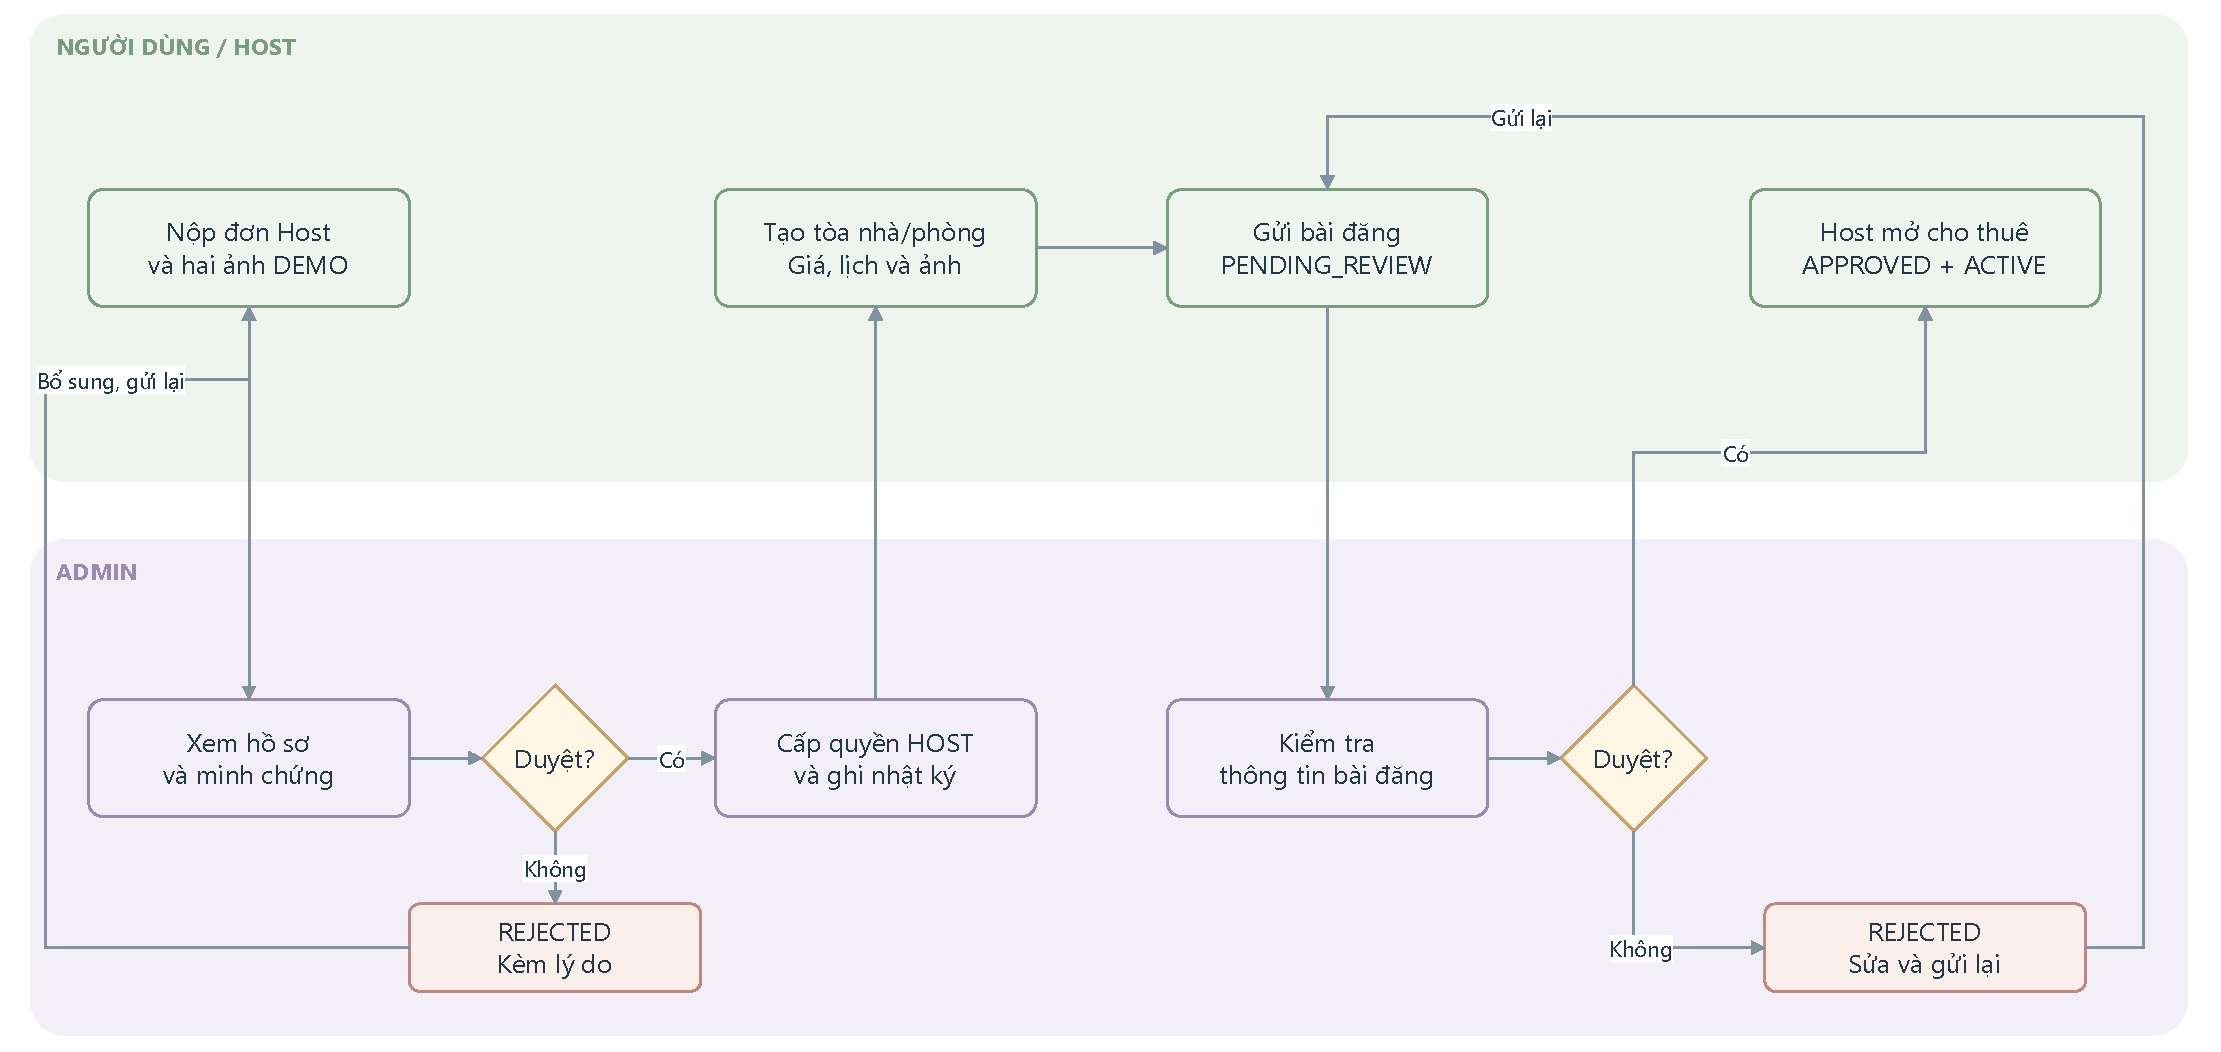
\includegraphics[page=1,width=\linewidth,height=0.82\textheight,keepaspectratio]{chapter2/workflow_diagram_v2.pdf}
\caption{Quy trình cấp quyền Host và công bố không gian.}\label{fig:app-host-workflow}
\end{figure}
\clearpage\BroomLandscapePagefalse\end{landscape}\pagestyle{fancy}
\clearpage
\begin{landscape}\pagestyle{empty}\BroomLandscapePagetrue
\begin{figure}[p]\centering
\includegraphics[page=2,width=\linewidth,height=0.82\textheight,keepaspectratio]{chapter2/workflow_diagram_v2.pdf}
\caption{Quy trình tạo, giữ lịch và xử lý yêu cầu đặt chỗ.}\label{fig:ch2-booking-workflow}
\end{figure}
\clearpage\BroomLandscapePagefalse\end{landscape}\pagestyle{fancy}
\clearpage
\begin{landscape}\pagestyle{empty}\BroomLandscapePagetrue
\begin{figure}[p]\centering
\includegraphics[page=3,width=\linewidth,height=0.82\textheight,keepaspectratio]{chapter2/workflow_diagram_v2.pdf}
\caption{Quy trình sử dụng phòng, khép lượt thuê và xác minh ngoại lệ.}\label{fig:app-usage-workflow}
\end{figure}
\clearpage\BroomLandscapePagefalse\end{landscape}\pagestyle{fancy}
\clearpage
\begin{landscape}\pagestyle{empty}\BroomLandscapePagetrue
\begin{figure}[p]\centering
\includegraphics[page=4,width=\linewidth,height=0.82\textheight,keepaspectratio]{chapter2/workflow_diagram_v2.pdf}
\caption{Luồng tạo QR và cập nhật kết quả thanh toán payOS.}\label{fig:app-payment-workflow}
\end{figure}
\clearpage\BroomLandscapePagefalse\end{landscape}\pagestyle{fancy}

\subsection{Sơ đồ phân rã chức năng}
Các chức năng được phân rã từ mục tiêu của từng vai trò đến nhóm thao tác liên quan. Nhóm người thuê bao gồm tài khoản, khám phá, booking, tương tác và hồ sơ Host; nhóm Host tập trung vào phòng, lịch và vận hành lượt thuê; nhóm Admin tập trung vào xét duyệt, xử lý vi phạm và kiểm tra nghiệp vụ. Cách phân rã tại Hình~\ref{fig:ch2-functions} làm rõ trách nhiệm mà không đồng nhất mỗi màn hình với một chức năng độc lập.

\begin{figure}[H]\centering
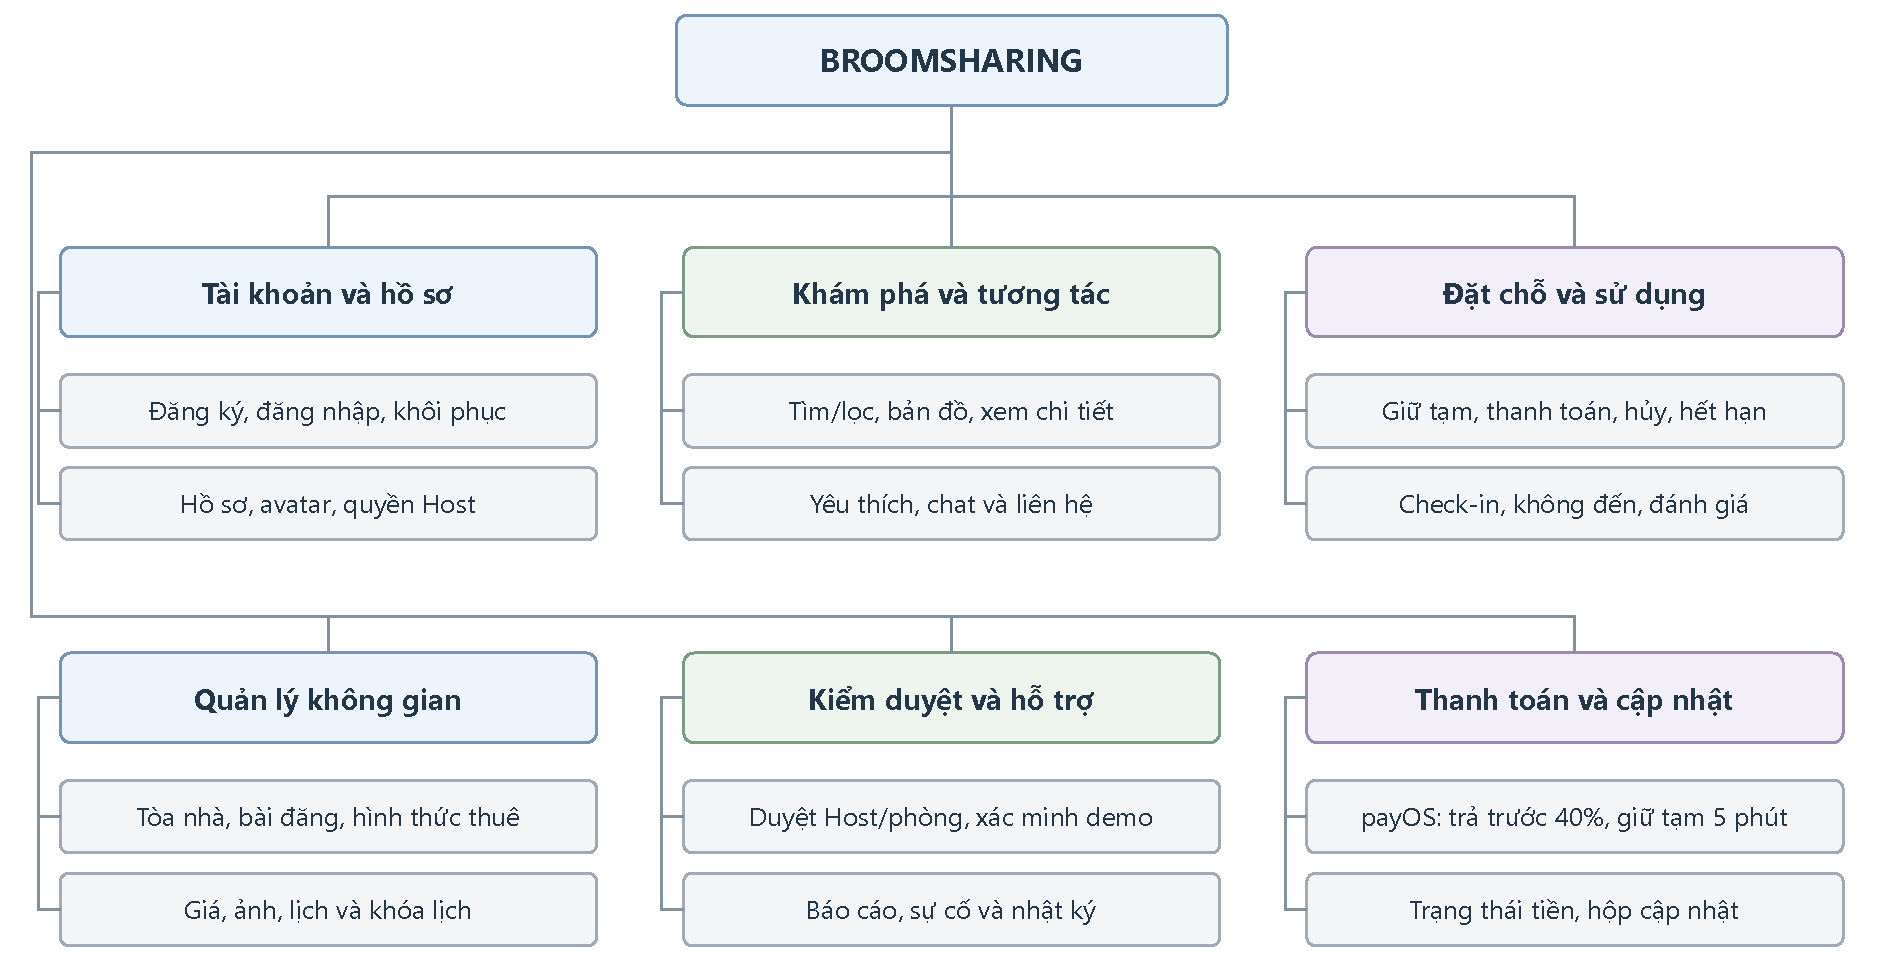
\includegraphics[page=1,width=\textwidth]{chapter2/usecase_decomposition_v2.pdf}
\caption{Phân rã chức năng tổng quát của BroomSharing.}\label{fig:ch2-functions}
\end{figure}

Chức năng tin nhắn hỗ trợ trao đổi giữa hai bên của một hội thoại. Hộp cập nhật tổng hợp sự kiện booking và trạng thái đã đọc của từng tài khoản. Đánh giá gắn với lượt đã sử dụng, còn báo cáo vi phạm được chuyển đến Admin và cho phép Host phản hồi. Các chức năng này bổ sung thông tin xử lý cho lượt thuê, đồng thời duy trì giới hạn truy cập theo vai trò và chủ thể liên quan.

Bộ phân rã chi tiết được lưu cùng tài nguyên đồ án tại \hyperref[app:project-resources]{Phụ lục C}.

\subsection{Sơ đồ use case}
Hình~\ref{fig:ch2-usecase-overview} mô tả các mục tiêu tương tác với hệ thống. Host kế thừa khả năng thuê phòng của người thuê và có thêm nhóm chức năng cho thuê. Admin có tuyến chức năng kiểm duyệt riêng; quyền quản trị không mặc định bao gồm đọc hội thoại riêng của người dùng.

\begin{figure}[H]\centering
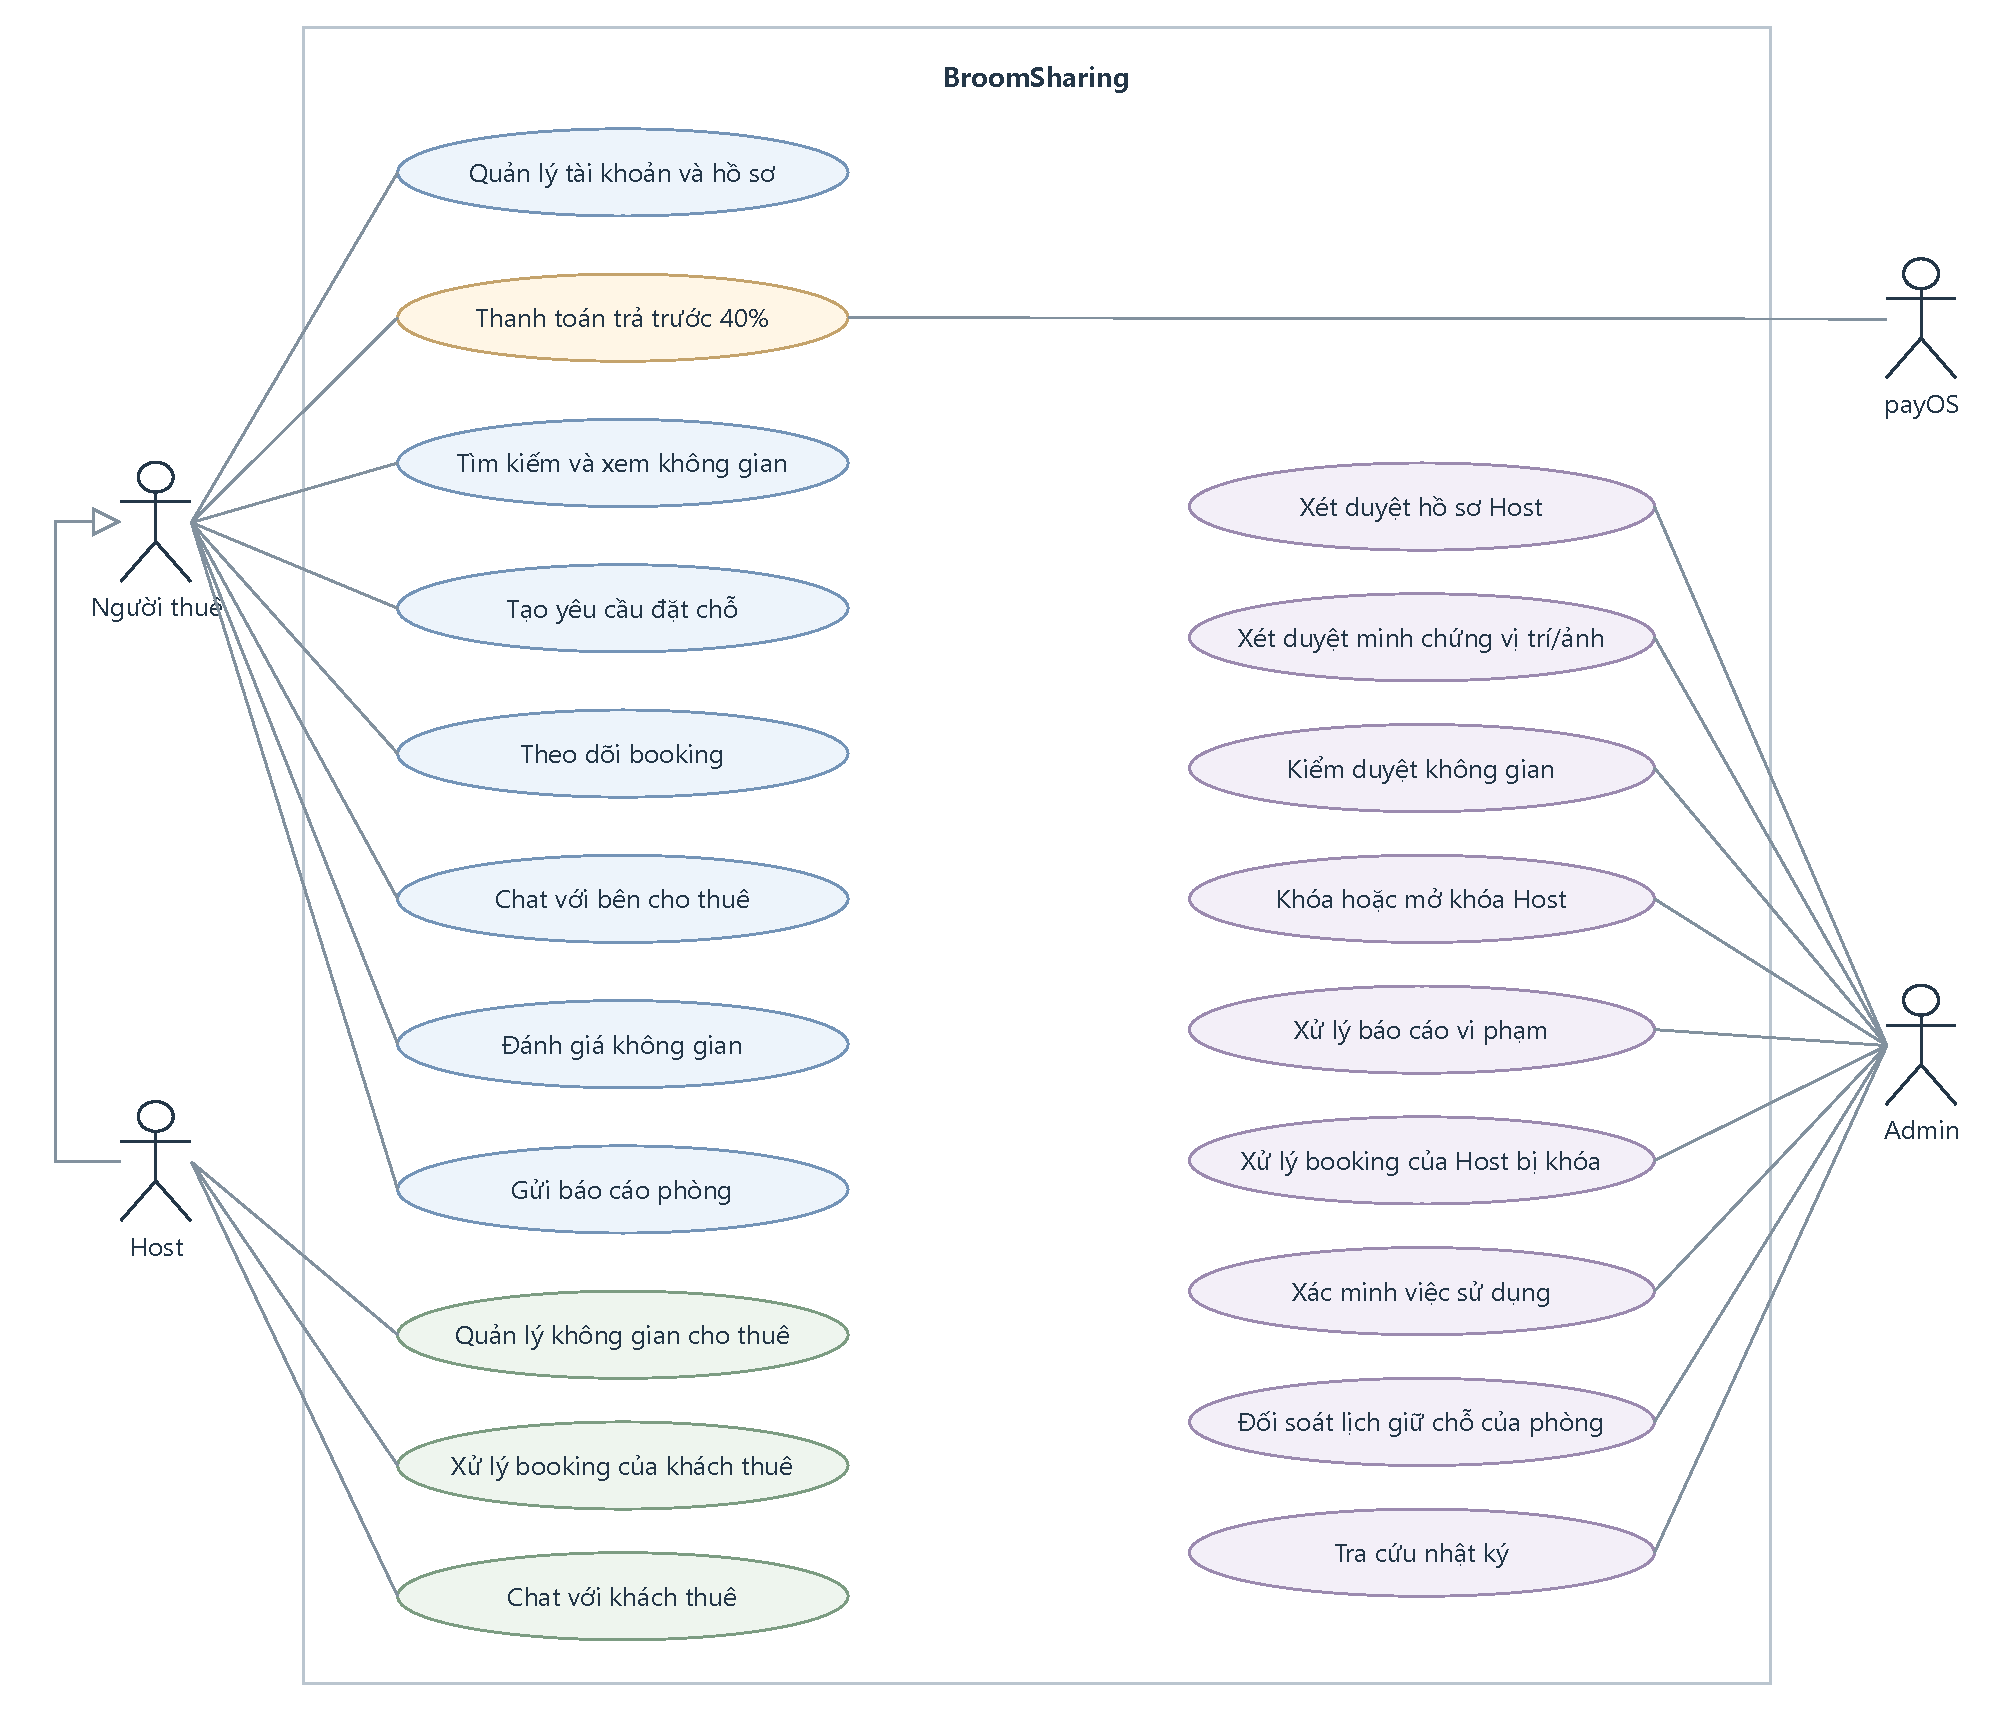
\includegraphics[page=1,width=0.95\textwidth]{chapter2/usecase_diagram_v2.pdf}
\caption{Use case tổng quát với các tác nhân người thuê, Host, Admin và dịch vụ thanh toán.}\label{fig:ch2-usecase-overview}
\end{figure}

Ở phân hệ người thuê, đặt chỗ luôn bao gồm kiểm tra khả dụng và mở bước thanh toán, còn hủy booking là thao tác có điều kiện trên lượt đang được theo dõi. Gửi đơn làm Host bao gồm cung cấp hai ảnh DEMO. Các phân hệ Host và Admin giữ liên kết tác nhân với mục tiêu nghiệp vụ; những cập nhật lịch và nhật ký được mô tả trong quy trình xử lý. Hình~\ref{fig:app-usecase-guest}, Hình~\ref{fig:app-usecase-host} và Hình~\ref{fig:app-usecase-admin} trình bày chi tiết mục tiêu của từng phân hệ.


Phân hệ người thuê bao quát truy cập tài khoản, khám phá, đặt chỗ và tương tác sau thuê. Kiểm tra khả dụng và mở thanh toán thuộc thao tác đặt chỗ; hủy booking chỉ thực hiện khi lượt thuê còn đáp ứng điều kiện hủy.
\begin{figure}[H]\centering
\includegraphics[page=2,width=\textwidth,height=0.75\textheight,keepaspectratio]{chapter2/usecase_diagram_v2.pdf}
\caption{Use case chi tiết của người thuê.}\label{fig:app-usecase-guest}
\end{figure}
Host quản lý tài sản, lịch và việc thực hiện lượt thuê; Admin xét duyệt, xử lý vi phạm và can thiệp booking trong phạm vi quản trị. Hình~\ref{fig:app-usecase-host} và Hình~\ref{fig:app-usecase-admin} thể hiện hai nhóm mục tiêu này. Quyền thuê chung của Host được kế thừa ở sơ đồ tổng quát; xác minh sử dụng và đối soát lịch là các mục tiêu quản trị riêng.

\begin{figure}[H]\centering
\begin{minipage}[t]{0.485\textwidth}\vspace{0pt}\centering
\includegraphics[page=3,width=\linewidth,height=0.67\textheight,keepaspectratio]{chapter2/usecase_diagram_v2.pdf}
\caption{Use case chi tiết của Host.}\label{fig:app-usecase-host}
\end{minipage}\hfill
\begin{minipage}[t]{0.485\textwidth}\vspace{0pt}\centering
\includegraphics[page=4,width=\linewidth,height=0.67\textheight,keepaspectratio]{chapter2/usecase_diagram_v2.pdf}
\caption{Use case chi tiết của Admin.}\label{fig:app-usecase-admin}
\end{minipage}
\end{figure}

\subsection{Ràng buộc nghiệp vụ và yêu cầu phi chức năng}
Các workflow trên chịu những ràng buộc tại Bảng~\ref{tab:ch2-constraints}. Mỗi thao tác được kiểm tra lại từ trạng thái hiện tại và quyền của người thực hiện; việc ẩn hoặc hiện nút trên màn hình không thay thế kiểm tra tại tầng dữ liệu.

\begin{table}[H]\centering\small
\caption{Các ràng buộc thiết kế chính}\label{tab:ch2-constraints}
\begin{tabularx}{\linewidth}{@{}p{3.2cm}X@{}}\toprule
Nhóm & Ràng buộc\\\midrule
Hình thức thuê & Mỗi phòng dùng HOURLY hoặc FIXED; FIXED thuê một hoặc ba tháng. Host chỉ đổi cấu hình khi không còn booking giữ chỗ.\\
Chống đặt trùng & Kiểm tra lại phòng và lịch trong transaction. Cùng request ID và nội dung trả lại booking đã tạo, tránh sinh lượt thuê lặp.\\
Giữ chỗ và tiền & PENDING tạm giữ tối đa 5 phút, không vượt giờ bắt đầu. Đủ 40\% đúng hạn mới xác nhận; quá hạn chưa trả thì nhả lịch, giữ lịch sử.\\
Khép lượt thuê & Xác minh sử dụng trước khi hoàn tất hoặc cho đánh giá; hủy, hết hạn hay kết thúc do sự cố phải nhả đúng khóa lịch, không thực hiện hai lần.\\
Quản trị & Khóa Host hoặc đình chỉ phòng ngăn nhận đặt mới, không xóa lịch sử. Gỡ đình chỉ đưa phòng về không hoạt động để Host kiểm tra trước khi mở lại.\\
Phân quyền & Kiểm tra UID, vai trò và quan hệ sở hữu tại Rules; backend thanh toán xác thực danh tính và lấy số tiền từ dữ liệu đã chốt \parencite{firebase_rules_conditions}.\\
Phản hồi giao diện & Phân biệt đang tải, trống, lỗi và thành công; giữ dữ liệu biểu mẫu phù hợp, nhận cập nhật và cho phép thử lại khi có lỗi kết nối.\\
\bottomrule\end{tabularx}
\end{table}

Báo cáo vi phạm và đánh giá có mục đích riêng: báo cáo chuyển tới Admin để xử lý, còn đánh giá phản ánh một lượt đã sử dụng. Việc can thiệp booking của Host bị khóa được thực hiện từng trường hợp và lưu lý do, không tự suy ra đã thu hoặc hoàn tiền.

\chapstart
\section{THIẾT KẾ GIAO DIỆN}
\subsection{Định hướng thiết kế}
Giao diện BroomSharing sử dụng xanh lục và xanh ngọc trên nền trắng, xám nhẹ; thống nhất tiêu đề, trường nhập, thẻ phòng và nút chính. Nội dung được mở dần từ danh sách đến chi tiết, thời gian và chi phí.

Các hình trong chương là prototype ban đầu trên Figma. Chúng thể hiện bố cục và hướng tương tác; giao diện hiện thực được trình bày ở Chương 5 và quy trình sử dụng ở Chương 6. Những lựa chọn hợp đồng hoặc phương thức đăng nhập trong prototype không đồng nghĩa đã được tích hợp vào ứng dụng.

\subsection{Giao diện người thuê}
\subsubsection{Đăng nhập và đăng ký}
Hình~\ref{fig:ch3-auth} nhóm trường tài khoản, mật khẩu và liên hệ theo thứ tự nhập; nút gửi biểu mẫu có màu nhấn, còn liên kết đăng ký và quên mật khẩu đặt riêng. Biểu tượng mật khẩu hỗ trợ kiểm tra nội dung nhập. Thiết kế dành phản hồi cho dữ liệu thiếu, sai định dạng hoặc xác thực không thành công, đồng thời giữ phần thông tin còn hợp lệ khi sửa lỗi.

\begin{figure}[H]\centering
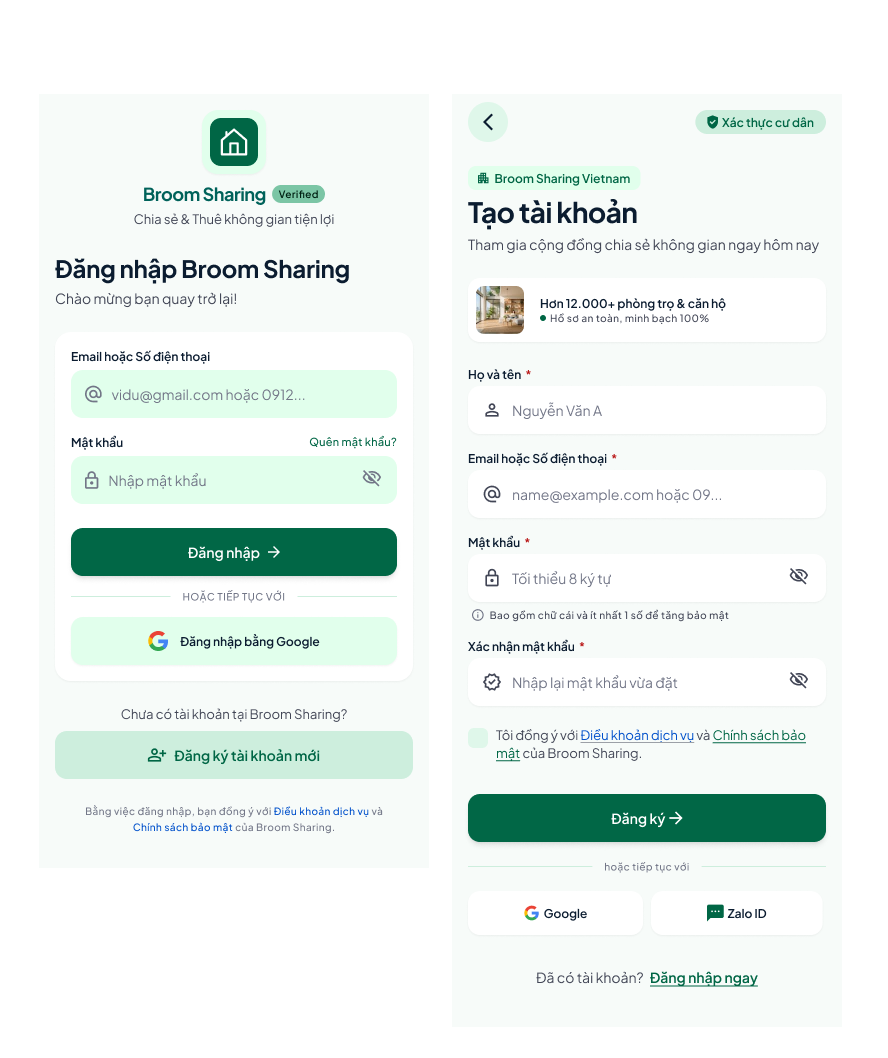
\includegraphics[width=0.9\textwidth,height=0.43\textheight,keepaspectratio]{chapter3/auth-design.png}
\caption{Thiết kế biểu mẫu đăng nhập và đăng ký tài khoản.}\label{fig:ch3-auth}
\end{figure}
\clearpage

\subsubsection{Trang chủ và chi tiết không gian}
Trang chủ trong Hình~\ref{fig:ch3-home} đặt tìm kiếm, danh mục và thẻ không gian theo thứ bậc; ảnh, tên, khu vực và đơn vị giá hỗ trợ so sánh nhanh. Thanh điều hướng đáy duy trì lối vào các nhóm chức năng. Danh sách hiện thực sử dụng RecyclerView để tái sử dụng View khi hiển thị \parencite{android_recycler}.

Chi tiết phòng tại Hình~\ref{fig:ch3-detail} mở rộng bộ ảnh, sức chứa, tiện ích, vị trí và thông tin Host thành các khối có thể cuộn. Yêu thích, nhắn tin, chỉ đường và đặt thuê gắn với phòng đang xem. Đơn vị giá đặt sát số tiền để phân biệt thuê giờ và kỳ thuê cố định.

\begin{figure}[H]\centering
\begin{minipage}[t]{0.31\textwidth}\centering
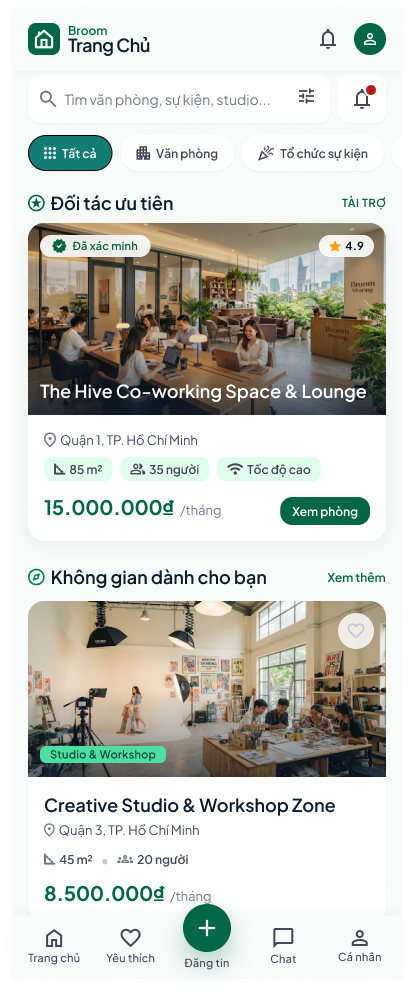
\includegraphics[width=\linewidth,height=0.53\textheight,keepaspectratio]{chapter3/home-design.png}
\caption{Thiết kế Trang chủ.}\label{fig:ch3-home}
\end{minipage}\hfill
\begin{minipage}[t]{0.65\textwidth}\centering
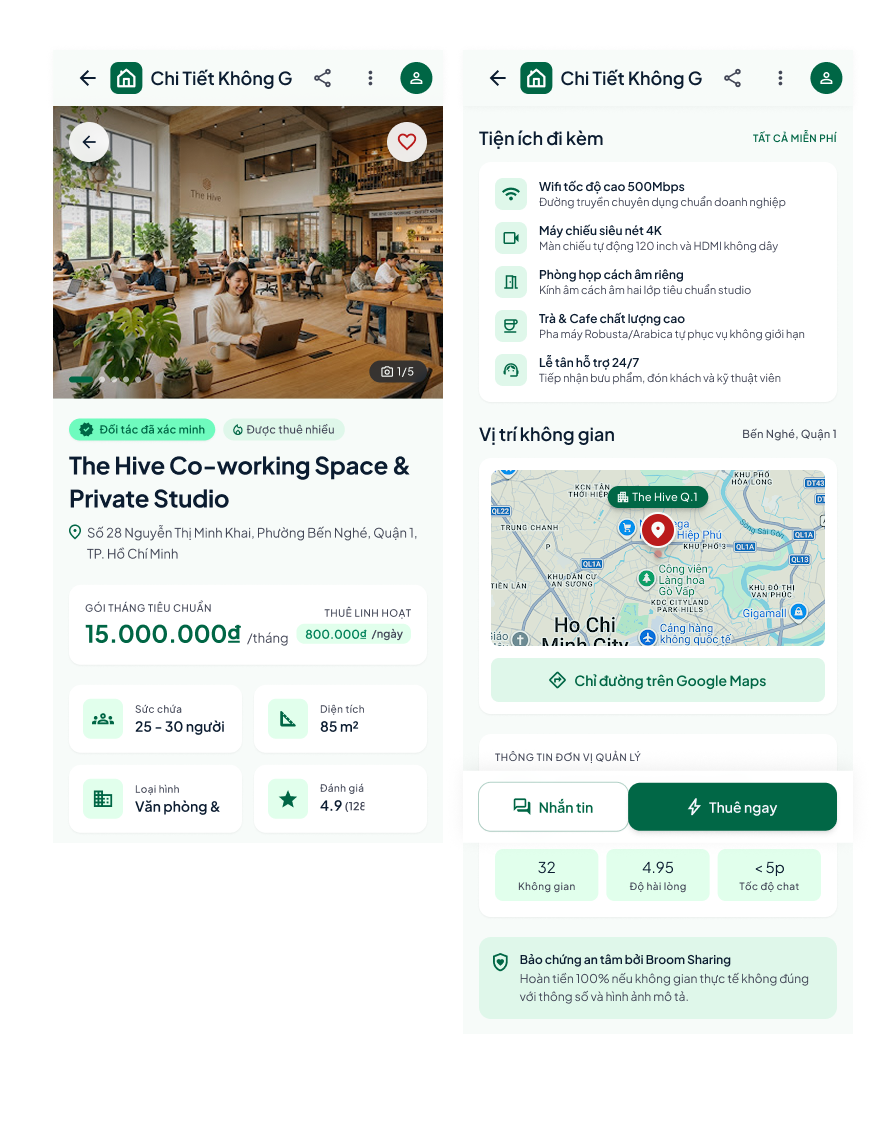
\includegraphics[trim=0 88 0 0,clip,width=\linewidth,height=0.53\textheight,keepaspectratio]{chapter3/detail-design.png}
\caption{Thiết kế thông tin chi tiết không gian.}\label{fig:ch3-detail}
\end{minipage}
\end{figure}
\clearpage

\subsubsection{Đặt chỗ và tương tác}
Hình~\ref{fig:app-booking-design} tập hợp phòng, thời gian, liên hệ và chi phí trước khi gửi yêu cầu. Tổng tiền và nút chính nằm cuối tiến trình; thay đổi thời gian phải cập nhật phần chi phí liên quan. Các lựa chọn hợp đồng, bảo chứng và tiền cọc trong hình thuộc phương án ban đầu, còn quy trình hiện thực tuân theo chính sách thanh toán của Chương 2.

\begin{figure}[H]\centering
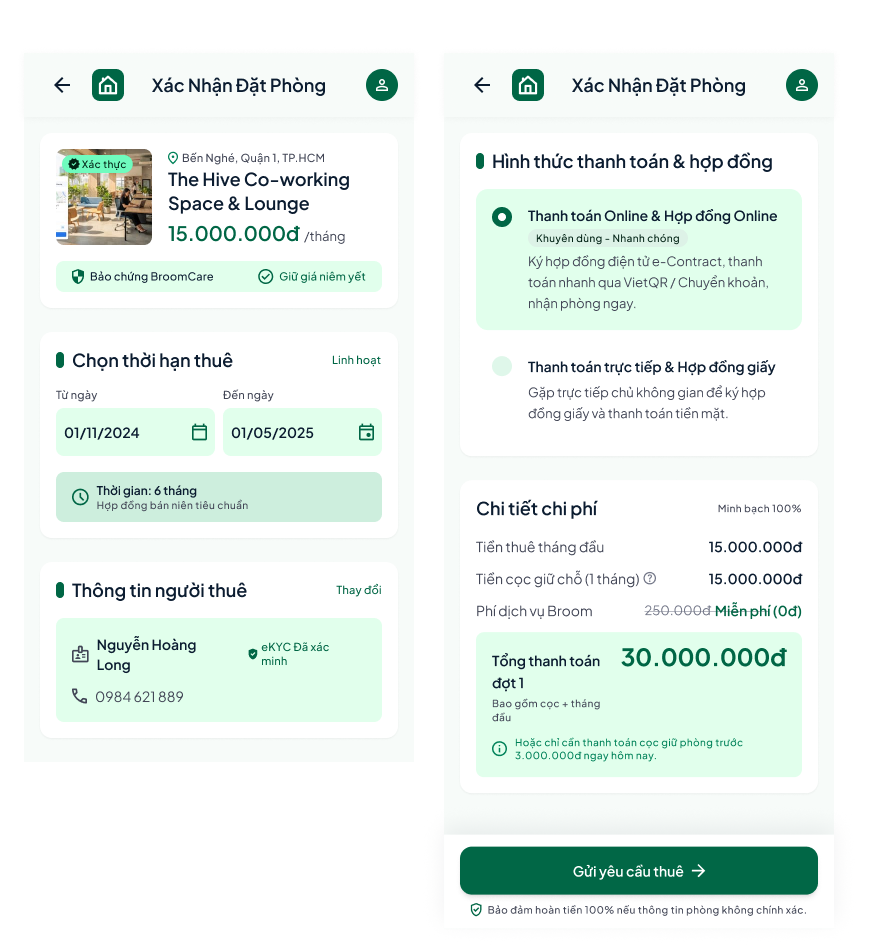
\includegraphics[width=\textwidth,height=0.56\textheight,keepaspectratio]{chapter3/booking-design.png}
\caption{Prototype xác nhận thông tin và chi phí đặt phòng.}\label{fig:app-booking-design}
\end{figure}

Hồ sơ phân nhóm thông tin cá nhân, ảnh đại diện, yêu thích và lịch sử. Hội thoại giữ ngữ cảnh phòng; hộp cập nhật dẫn về đúng lượt thuê liên quan. Đánh giá gắn với lượt đã xác nhận sử dụng, trong khi báo cáo vi phạm có biểu mẫu riêng gửi Admin.
\clearpage

\subsection{Giao diện chủ không gian}
Biểu mẫu Host tại Hình~\ref{fig:ch3-host} chia ba bước: thông tin cơ bản, giá và lịch, hình ảnh và điều kiện sử dụng. Thanh tiến trình cùng nút quay lại, tiếp tục cho phép kiểm tra nội dung trước khi gửi; dữ liệu cần được giữ khi chuyển giữa các bước. Vùng ảnh phân biệt tệp đã chọn, đang tải và lỗi tải.

\begin{figure}[H]\centering
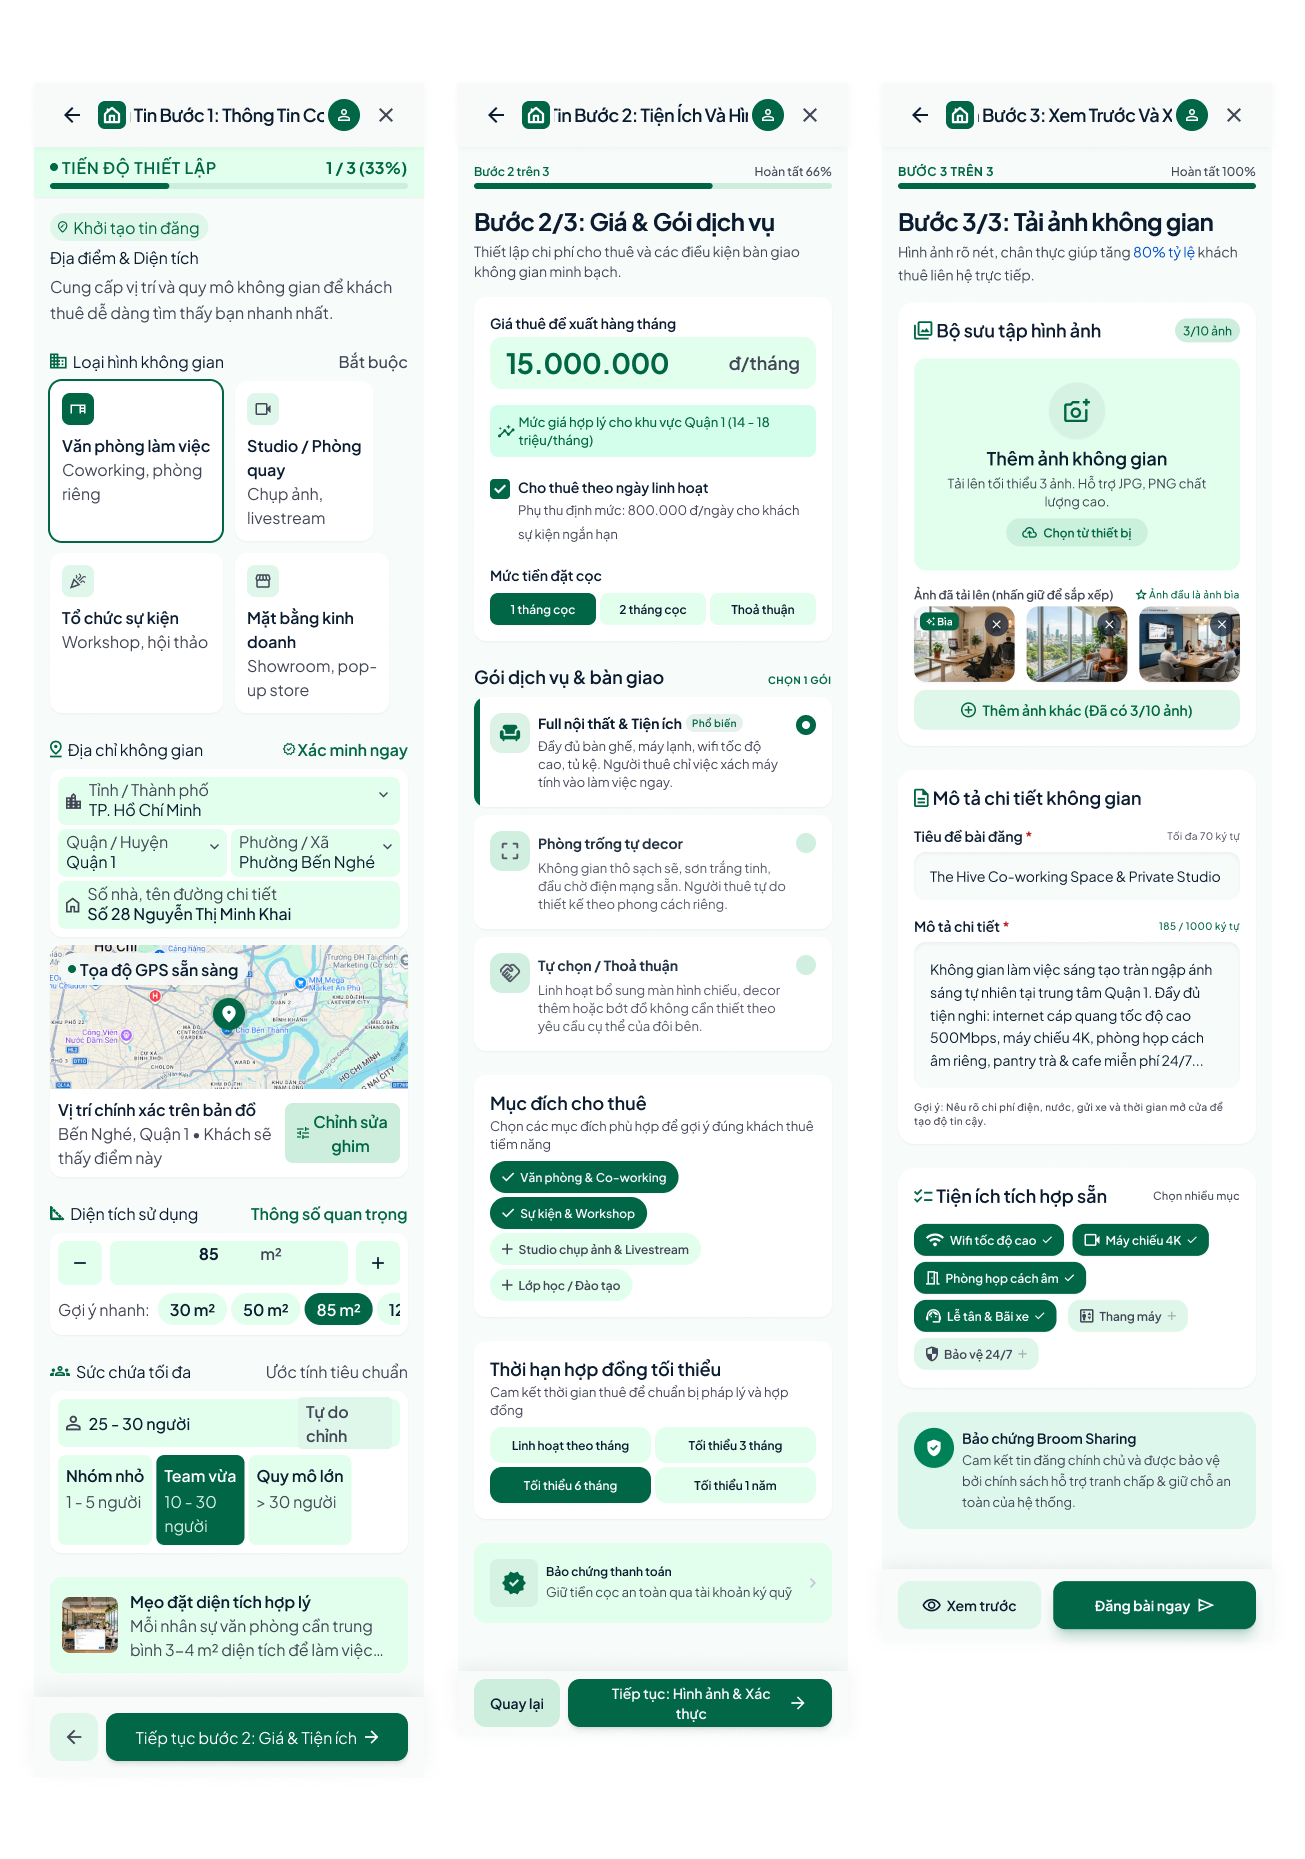
\includegraphics[width=\textwidth,height=0.48\textheight,keepaspectratio]{chapter3/host-design.png}
\caption{Prototype ba bước nhập thông tin và đăng không gian.}\label{fig:ch3-host}
\end{figure}

Khu vực quản lý tập trung phòng, booking và lịch. Nhãn chờ duyệt khác nhãn tạm ngừng; các thao tác nhận phòng, hoàn tất, không đến hoặc hủy được hiển thị theo trạng thái. Hành động ảnh hưởng lượt thuê cần xác định đúng đối tượng và yêu cầu lý do khi phù hợp.

\subsection{Giao diện quản trị viên}
Admin được tổ chức thành tổng quan, xét duyệt, quản lý và báo cáo. Bộ lọc giúp chọn loại hồ sơ, còn quyết định chấp thuận hoặc từ chối gắn với thẻ đang xem. Đơn cấp quyền Host độc lập với minh chứng vị trí, hình ảnh. Prototype trong Hình~\ref{fig:app-admin-design} ở Phụ lục B minh họa cách nhóm thông tin và thao tác này; các con số chỉ phục vụ thiết kế bố cục.

\chapstart
\section{THIẾT KẾ CƠ SỞ DỮ LIỆU}
\label{sec:database-design}
\begingroup
\setlist[itemize]{leftmargin=1.27cm,label=\textbullet,itemsep=2pt,topsep=4pt}
\setlist[enumerate]{leftmargin=1.27cm,itemsep=2pt,topsep=4pt}
\setlength{\emergencystretch}{1em}
\widowpenalty=10000
\clubpenalty=10000

BroomSharing sử dụng database \texttt{broomsharing} của Cloud Firestore để lưu dữ liệu tài khoản, không gian, đặt chỗ và trao đổi giữa các bên. Firebase Authentication quản lý danh tính đăng nhập, liên kết với hồ sơ người dùng qua UID. Cloudinary lưu ảnh và minh chứng DEMO, còn Firestore giữ URL tham chiếu. Backend Java quản lý giao dịch payOS và trạng thái tiền \parencite{broomsharing_source}.

\subsection{Các thực thể và thuộc tính}
\label{sec:ch4-entities}

Dữ liệu ứng dụng được tổ chức thành 17 collection gốc và ba loại subcollection, tương ứng 20 mẫu document đang được ứng dụng hoặc backend sử dụng trong Bảng~\ref{tab:ch4-entities-summary}. Các thuộc tính định danh liên kết tài khoản với tài sản và yêu cầu thuê; nhóm trạng thái chi phối việc công bố phòng, xét duyệt và chuyển bước đặt chỗ. Collection thông báo cũ chỉ còn contract trong Rules, không phải nguồn hộp cập nhật đang hoạt động. Document còn chứa dữ liệu nhúng dạng \texttt{map}, \texttt{array} và các mốc thời gian xử lý. Những trường như người duyệt hoặc thời điểm hủy chỉ phát sinh khi nghiệp vụ tương ứng được thực hiện.

\begingroup\small\setstretch{1.06}
\begin{longtable}{@{}>{\raggedright\arraybackslash}p{3.6cm}>{\raggedright\arraybackslash}p{3.75cm}>{\raggedright\arraybackslash}p{7.9cm}@{}}
\caption{Các mẫu document và thuộc tính tiêu biểu}\label{tab:ch4-entities-summary}\\
\toprule Đường dẫn & Vai trò & Thuộc tính tiêu biểu và kiểu \\ \midrule\endfirsthead
\toprule Đường dẫn & Vai trò & Thuộc tính tiêu biểu và kiểu \\ \midrule\endhead
\midrule\multicolumn{3}{r}{\small Còn tiếp ở trang sau}\\\endfoot
\bottomrule\endlastfoot
\texttt{users/\allowbreak{}\{\allowbreak{}uid\}} & Hồ sơ và quyền tài khoản. & \texttt{uid}, \texttt{role}, \texttt{status}, \texttt{photo\allowbreak{}Url} (\texttt{string}); \ldots \\
\texttt{public\allowbreak{}Hosts/\allowbreak{}\{\allowbreak{}uid\}} & Bản chiếu Host. & \texttt{uid}, \texttt{name}, \texttt{photo\allowbreak{}Url} (\texttt{string}); \ldots \\
\texttt{usernames/\allowbreak{}\{\allowbreak{}normalized\allowbreak{}Username\}} & Ánh xạ đăng nhập. & \texttt{uid}, \texttt{email} (\texttt{string}). \\
\texttt{host\allowbreak{}Applications/\allowbreak{}\{\allowbreak{}uid\}} & Đơn cấp quyền Host. & \texttt{applicant\allowbreak{}Uid}, \texttt{status} (\texttt{string}); \texttt{identity\allowbreak{}Image\allowbreak{}Urls} (\texttt{array\textless{}\allowbreak{}string\textgreater{}}); \ldots \\
\texttt{users/\allowbreak{}\{\allowbreak{}uid\}\allowbreak{}/\allowbreak{}favorites/\allowbreak{}\{\allowbreak{}room\allowbreak{}Id\}} & Phòng yêu thích. & \texttt{room\allowbreak{}Id}, \texttt{room\allowbreak{}Name} (\texttt{string}); \texttt{created\allowbreak{}At} (\texttt{timestamp}). \\
\texttt{users/\allowbreak{}\{\allowbreak{}uid\}\allowbreak{}/\allowbreak{}notice\allowbreak{}Reads/\allowbreak{}\{\allowbreak{}event\allowbreak{}Id\}} & Mốc đọc sự kiện dẫn xuất. & \texttt{read\allowbreak{}At} (\texttt{timestamp}). \\
\texttt{buildings/\allowbreak{}\{\allowbreak{}building\allowbreak{}Id\}} & Địa điểm và chủ sở hữu. & \texttt{owner\allowbreak{}Uid}, \texttt{name}, \texttt{address} (\texttt{string}); \texttt{location} (\texttt{geopoint/\allowbreak{}null}); \ldots \\
\texttt{rooms/\allowbreak{}\{\allowbreak{}room\allowbreak{}Id\}} & Không gian và trạng thái tin. & \texttt{building\allowbreak{}Id}, \texttt{owner\allowbreak{}Uid}, \texttt{active\allowbreak{}Mode} (\texttt{string}); \texttt{active\allowbreak{}Booking\allowbreak{}Count} (\texttt{integer}); \ldots \\
\texttt{bookings/\allowbreak{}\{\allowbreak{}booking\allowbreak{}Id\}} & Kỳ thuê, trạng thái và giá đã chốt. & \texttt{room\allowbreak{}Id}, \texttt{guest\allowbreak{}Uid}, \texttt{status}, \texttt{payment\allowbreak{}Flow} (\texttt{string}); \texttt{price\allowbreak{}Snapshot} (\texttt{map}); \ldots \\
\texttt{availability\allowbreak{}Months/\allowbreak{}\{\allowbreak{}room\allowbreak{}Id\_\allowbreak{}yyyy\allowbreak{}MM\}} & Khóa lịch chính thức và tạm giữ. & \texttt{fixed\allowbreak{}Booking\allowbreak{}Id} (\texttt{string}); \texttt{slots\allowbreak{}Busy} (\texttt{array\textless{}\allowbreak{}integer\textgreater{}}); \texttt{hourly\allowbreak{}Bookings} (\texttt{map\textless{}\allowbreak{}string,\allowbreak{}array\textless{}\allowbreak{}integer\textgreater{}\allowbreak{}\textgreater{}}); \texttt{pending\allowbreak{}Payment\allowbreak{}Ids} (\texttt{array\textless{}\allowbreak{}string\textgreater{}}); \ldots \\
\texttt{payments/\allowbreak{}\{\allowbreak{}booking\allowbreak{}Id\}} & Giao dịch trả trước. & \texttt{order\allowbreak{}Code}, \texttt{amount}, \texttt{expires\allowbreak{}At} (\texttt{integer}); \texttt{status} (\texttt{string}); \ldots \\
\texttt{payment\allowbreak{}Orders/\allowbreak{}\{\allowbreak{}order\allowbreak{}Code\}} & Ánh xạ mã đơn của backend. & \texttt{booking\allowbreak{}Id} (\texttt{string}). \\
\texttt{app\allowbreak{}Config/\allowbreak{}payments} & Cấu hình kênh demo công khai. & \texttt{flow}, \texttt{demo\allowbreak{}Host\allowbreak{}Uid} (\texttt{string}). \\
\texttt{reviews/\allowbreak{}\{\allowbreak{}booking\allowbreak{}Id\}} & Đánh giá sau sử dụng. & \texttt{room\allowbreak{}Id}, \texttt{guest\allowbreak{}Uid}, \texttt{comment} (\texttt{string}); \texttt{rating} (\texttt{integer}); \ldots \\
\texttt{conversations/\allowbreak{}\{\allowbreak{}guest\allowbreak{}Uid:host\allowbreak{}Uid\}} & Hội thoại và mốc đọc. & \texttt{member\allowbreak{}Uids} (\texttt{array\textless{}\allowbreak{}string\textgreater{}}); \texttt{sequence}, \texttt{guest\allowbreak{}Read}, \texttt{host\allowbreak{}Read} (\texttt{integer}); \ldots \\
\texttt{conversations/\allowbreak{}\{\allowbreak{}guest\allowbreak{}Uid:host\allowbreak{}Uid\}\allowbreak{}/\allowbreak{}messages/\allowbreak{}\{\allowbreak{}message\allowbreak{}Id\}} & Tin nhắn của hội thoại. & \texttt{sender\allowbreak{}Uid}, \texttt{text} (\texttt{string}); \texttt{sequence} (\texttt{integer}); \texttt{created\allowbreak{}At} (\texttt{timestamp}); \ldots \\
\texttt{property\allowbreak{}Verifications/\allowbreak{}\{\allowbreak{}verification\allowbreak{}Id\}} & Minh chứng xác minh. & \texttt{owner\allowbreak{}Uid}, \texttt{verification\allowbreak{}Type}, \texttt{status} (\texttt{string}); \texttt{evidence\allowbreak{}Refs} (\texttt{array\textless{}\allowbreak{}string\textgreater{}}); \ldots \\
\texttt{reports/\allowbreak{}\{\allowbreak{}report\allowbreak{}Id\}} & Phản ánh và kết quả xử lý. & \texttt{reporter\allowbreak{}Uid}, \texttt{room\allowbreak{}Id}, \texttt{booking\allowbreak{}Id}, \texttt{status} (\texttt{string}); \ldots \\
\texttt{audit\allowbreak{}Logs/\allowbreak{}\{\allowbreak{}audit\allowbreak{}Id\}} & Dấu vết thay đổi. & \texttt{actor\allowbreak{}Uid}, \texttt{target\allowbreak{}Path}, \texttt{action} (\texttt{string}); \texttt{before}, \texttt{after} (\texttt{map\textless{}\allowbreak{}string,\allowbreak{}any\textgreater{}}); \ldots \\
\texttt{rental\allowbreak{}Places/\allowbreak{}\{\allowbreak{}place\allowbreak{}Id\}} & Địa điểm tham khảo, không đặt thuê. & \texttt{name}, \texttt{source\allowbreak{}Url} (\texttt{string}); \texttt{location} (\texttt{geopoint}); \ldots \\
\end{longtable}\endgroup


Mô hình tách hồ sơ tài khoản khỏi bản chiếu Host, thông tin phòng khỏi lịch giữ chỗ và nội dung hội thoại khỏi từng tin nhắn. Các lớp tổng hợp phục vụ giao diện như \texttt{Room\allowbreak{}Listing}, \texttt{Booking\allowbreak{}Notice} và \texttt{Host\allowbreak{}Stats} không có collection độc lập. Trong booking, tên phòng, liên hệ người thuê và giá được lưu tại thời điểm đặt, duy trì ngữ cảnh của yêu cầu khi dữ liệu gốc thay đổi.

Bản sao ngoại tuyến được lưu riêng trong SQLite trên thiết bị, không tạo thêm collection Firestore. Cấu trúc lưu cục bộ và cách cập nhật bản sao được trình bày tại Mục~\ref{sec:sqlite-offline}.

\subsection{Quan hệ dữ liệu và cấu trúc lưu trữ}
\label{sec:ch4-relationships}

Hình~\ref{fig:ch4-overview} thể hiện cây lưu trữ của hệ thống. Hai subcollection \texttt{favorites}, \texttt{notice\allowbreak{}Reads} thuộc từng document người dùng; \texttt{messages} thuộc từng document hội thoại. Các collection \texttt{buildings}, \texttt{rooms}, \texttt{bookings} và \texttt{availability\allowbreak{}Months} nằm ngang cấp, liên kết bằng các trường ID dạng chuỗi. Cấu trúc phân cấp này tuân theo mô hình collection và document của Firestore \parencite{firebase_data_model}.

% Original Page-2 through Page-6. Full vector figures; no redrawing/cropping.
\begin{figure}[H]
\centering
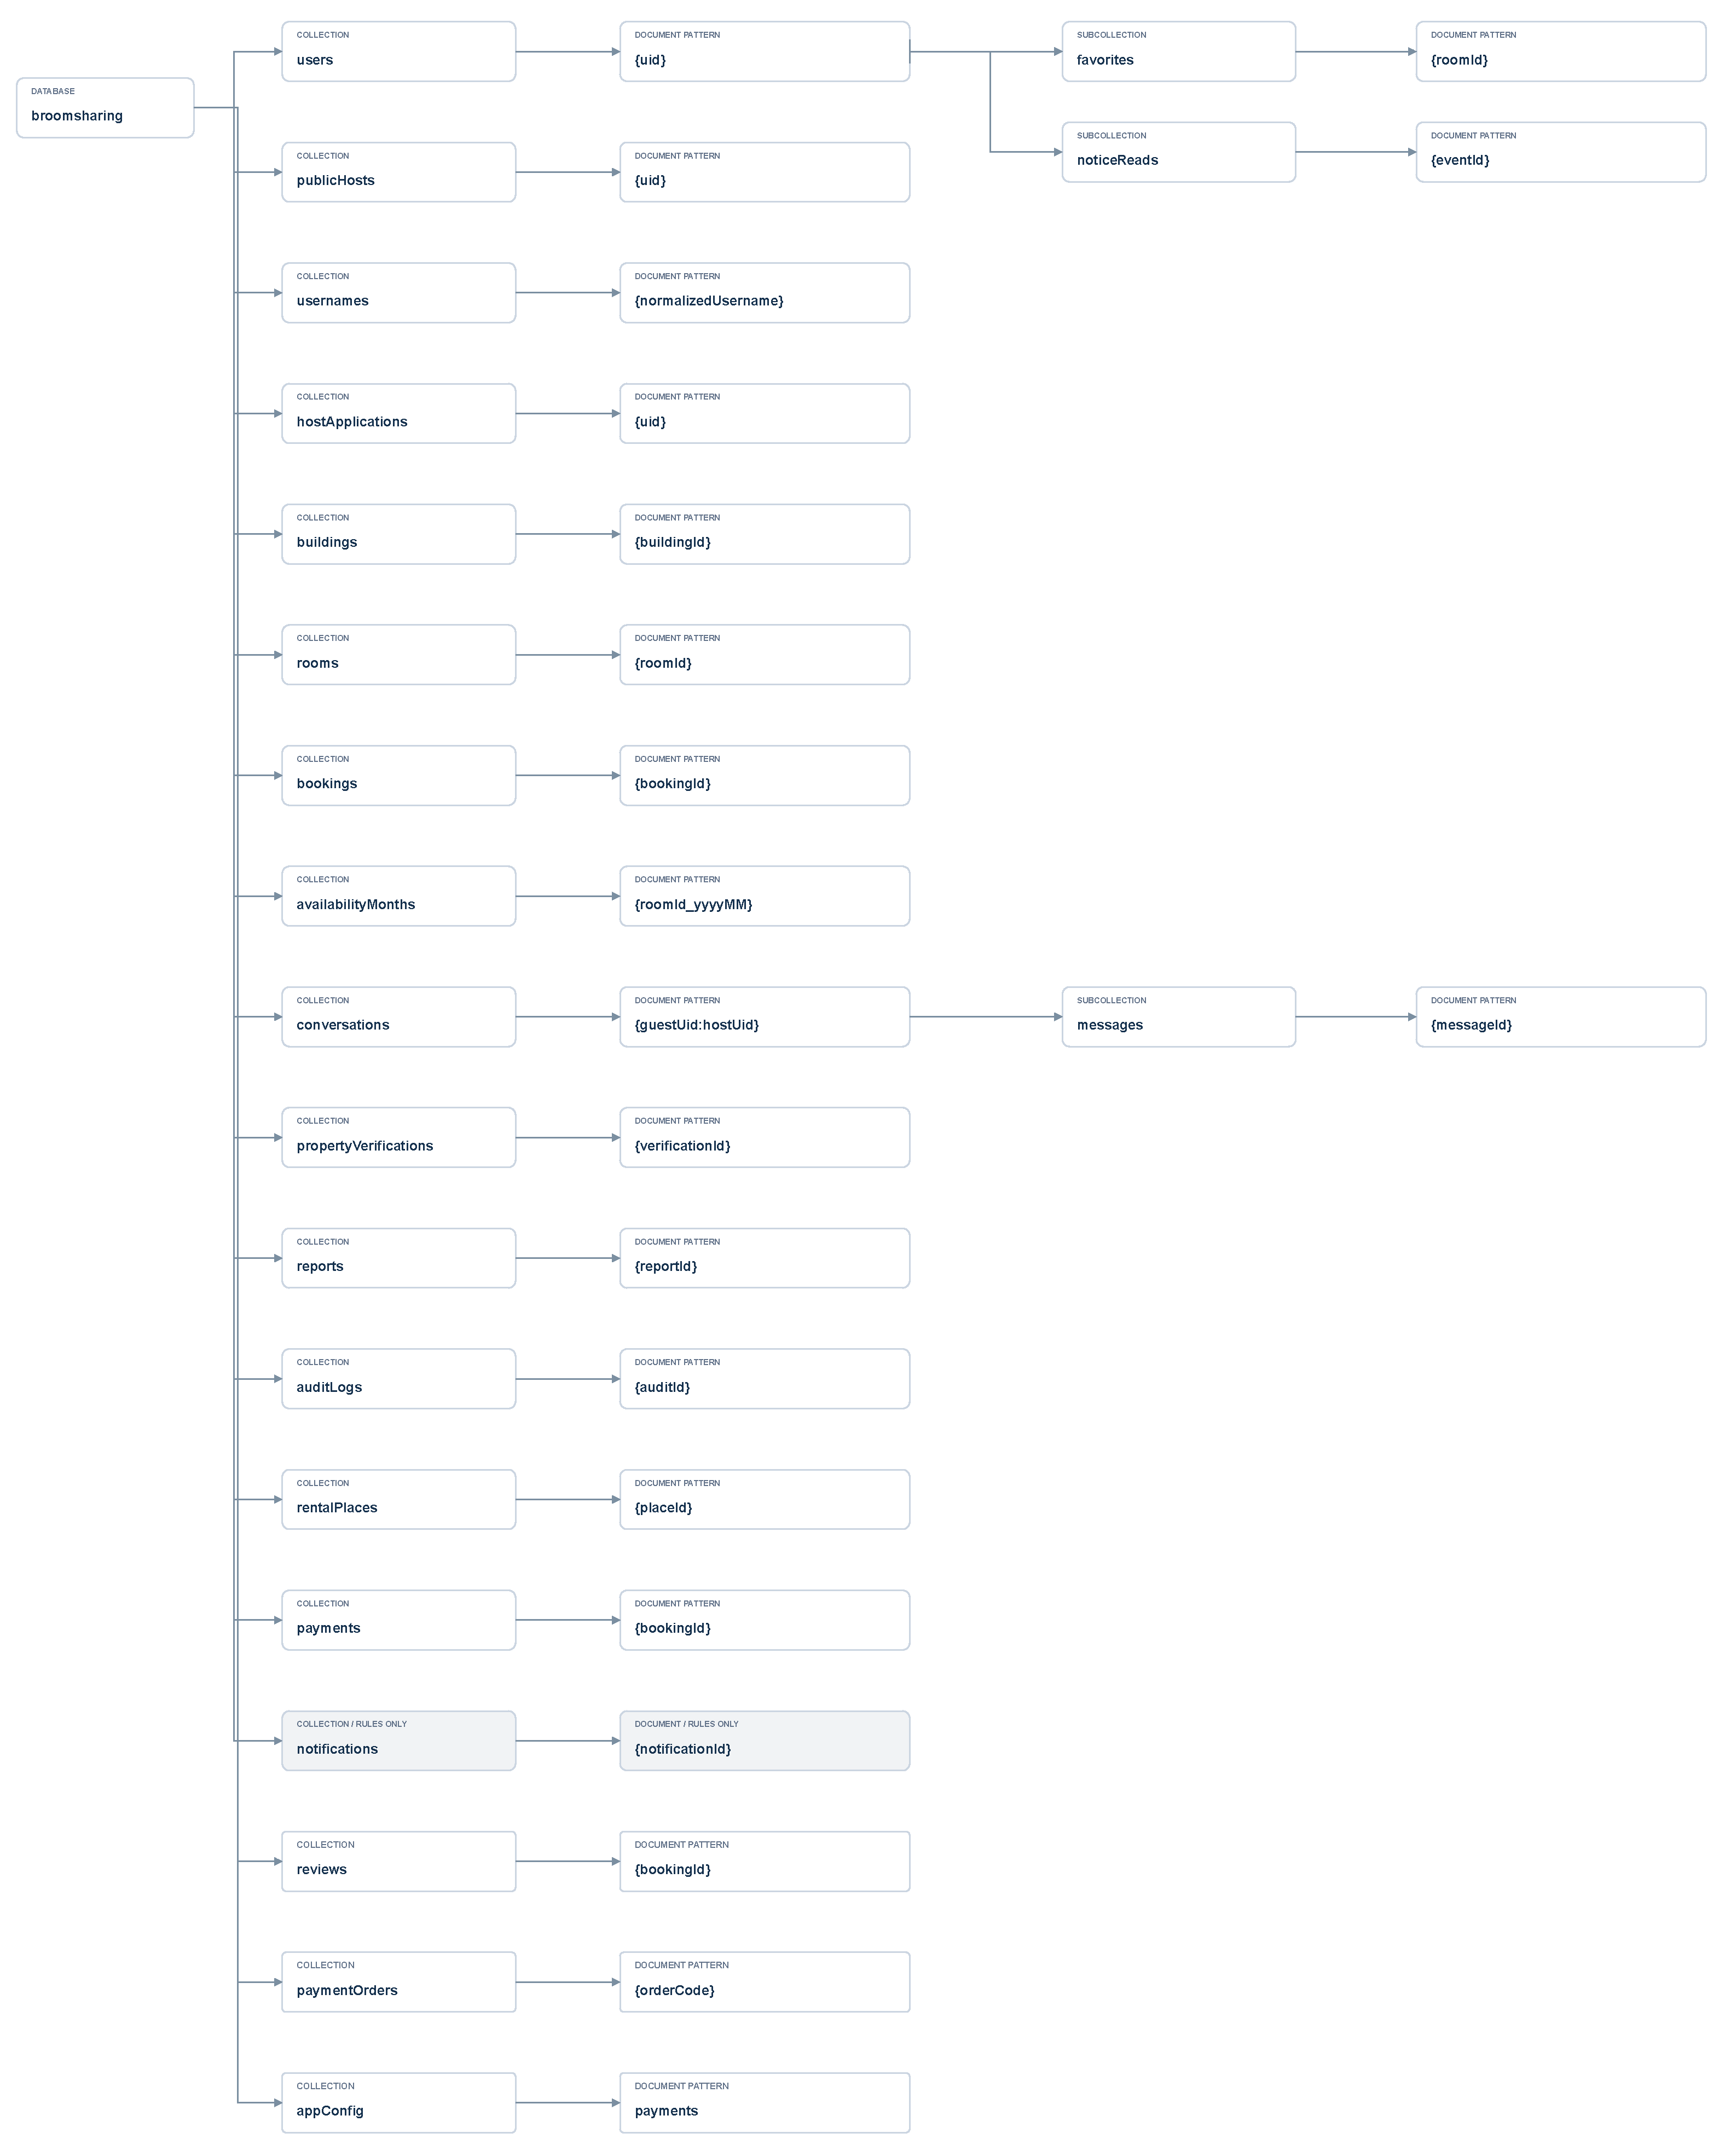
\includegraphics[width=\textwidth,height=0.86\textheight,keepaspectratio]{chapter4/firestore-overview.pdf}
\caption{Cây lưu trữ Firestore BroomSharing. Thẻ màu xám là contract thông báo cũ trong Rules.}
\label{fig:ch4-overview}
\end{figure}
\clearpage
\begin{landscape}
\pagestyle{empty}
\BroomLandscapePagetrue
\begin{figure}[p]
\centering
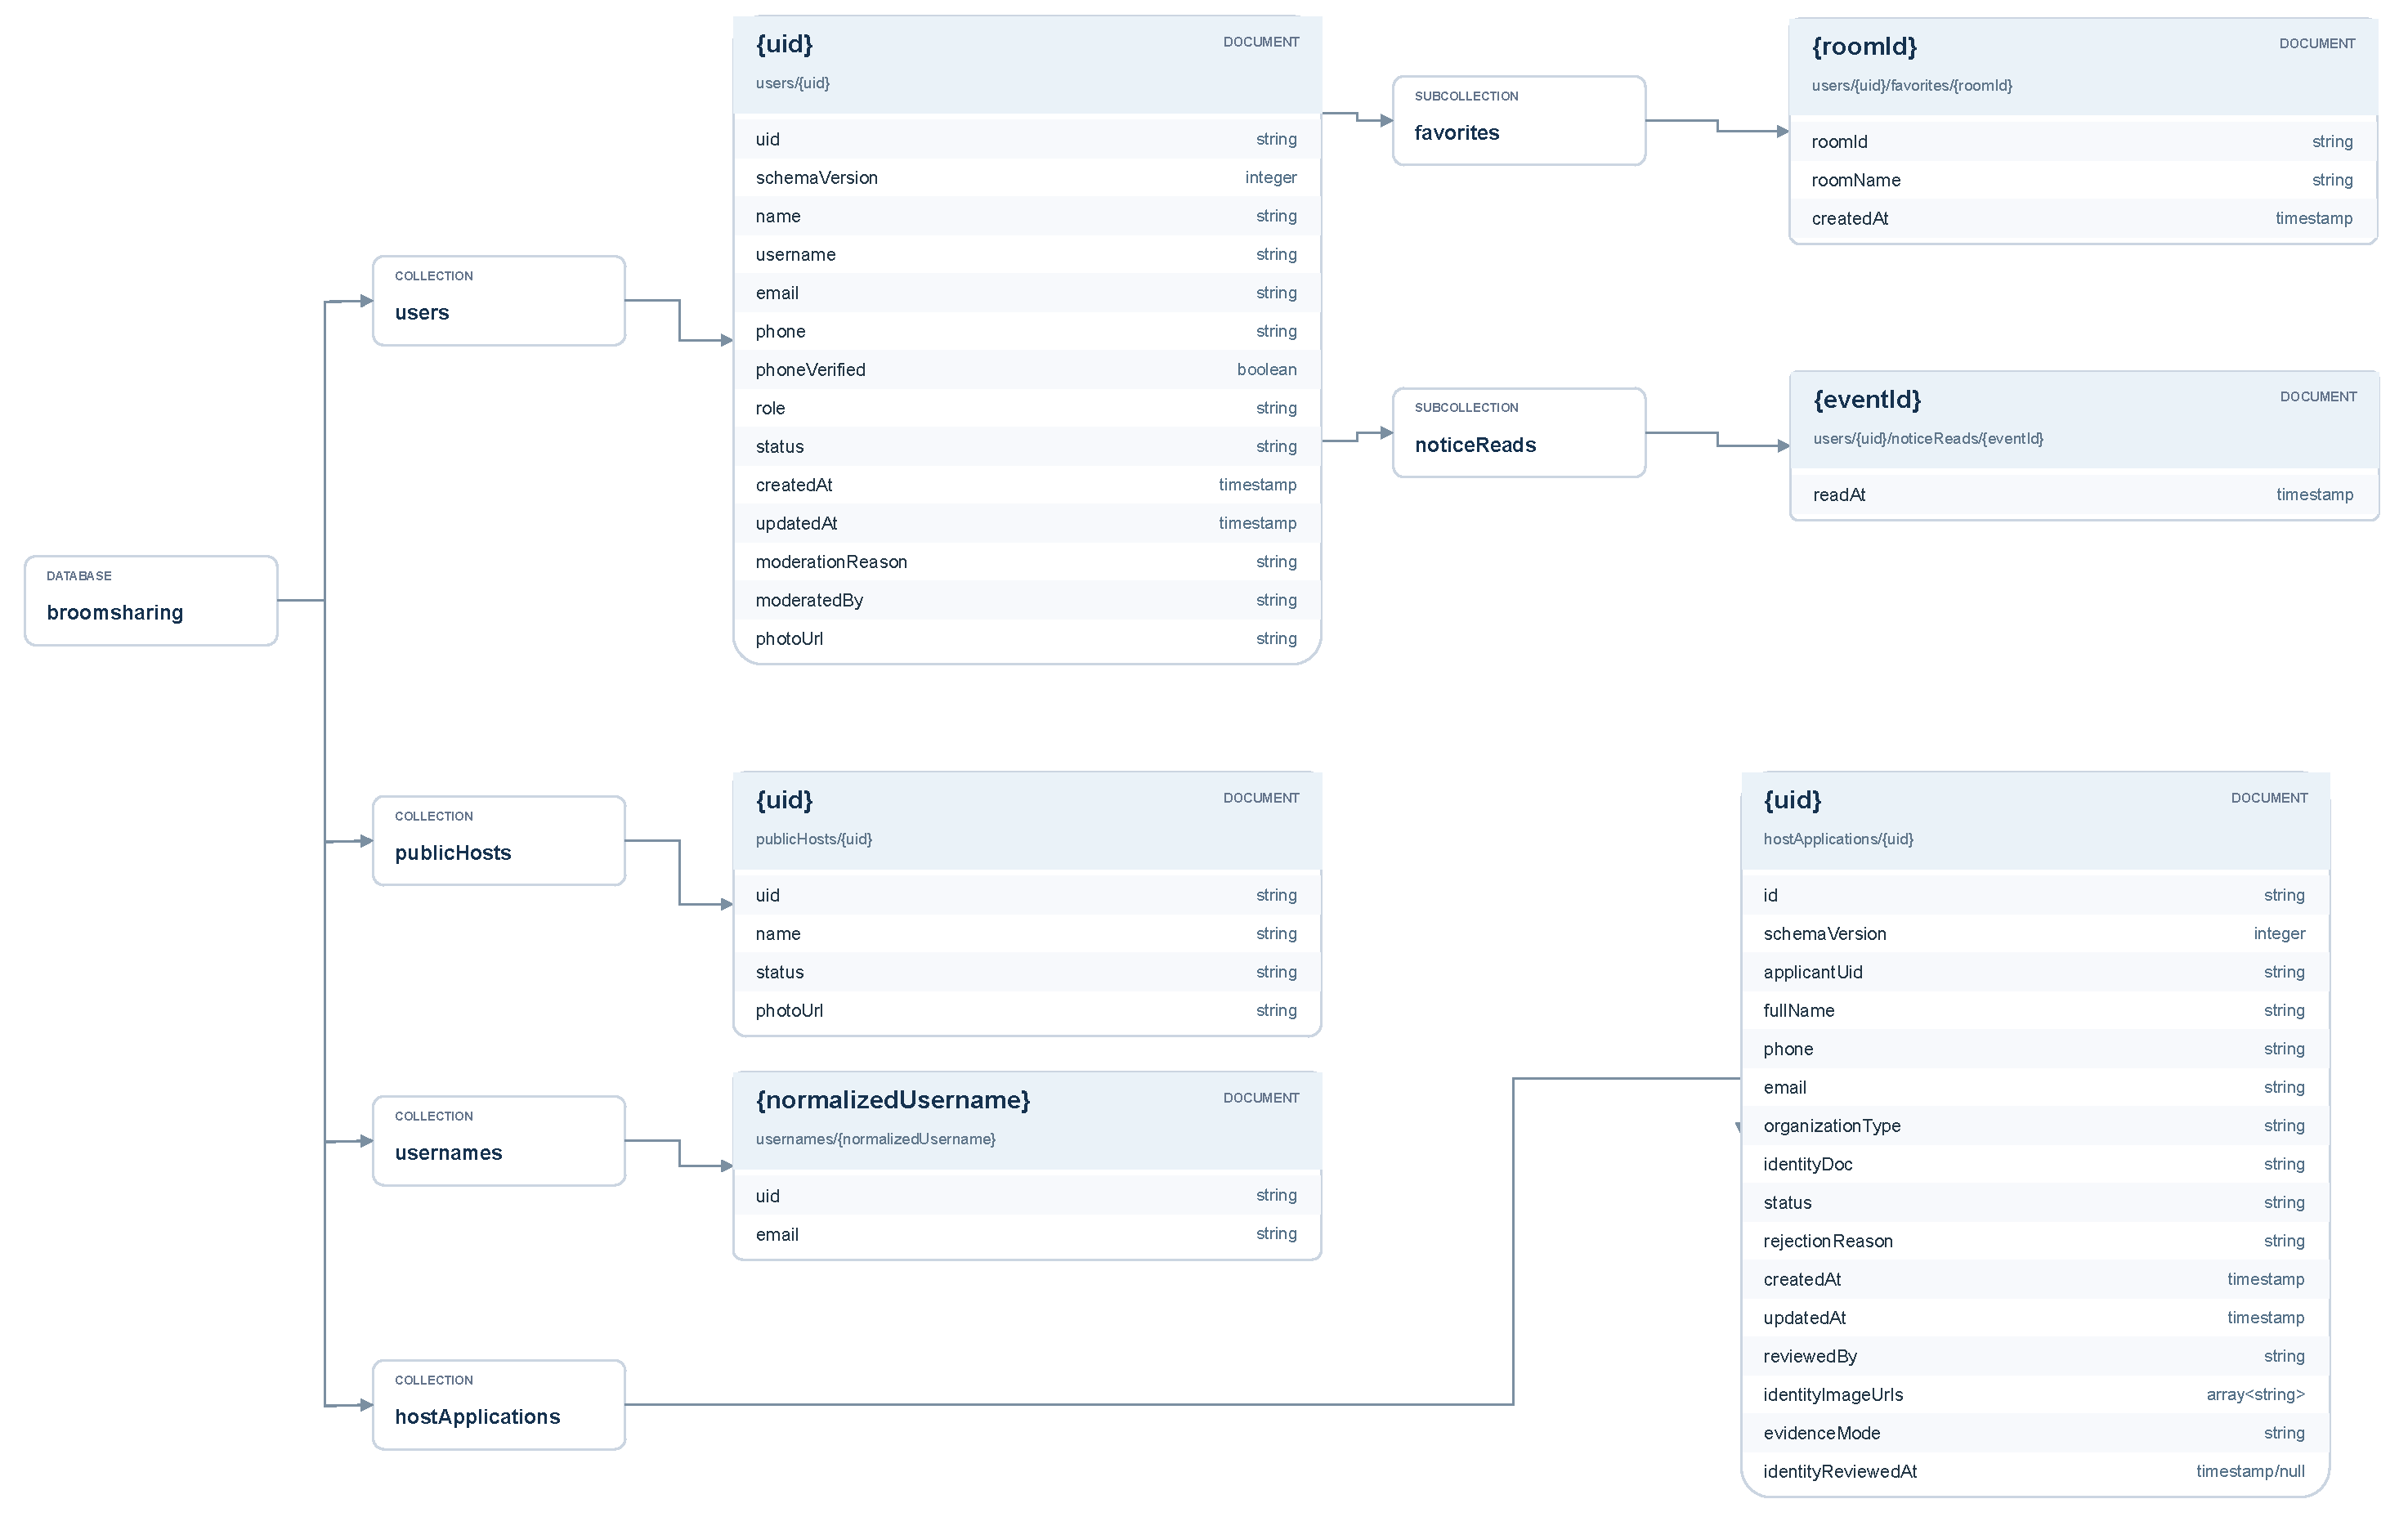
\includegraphics[width=\linewidth,height=0.82\textheight,keepaspectratio]{chapter4/firestore-accounts.pdf}
\caption{Cấu trúc nhóm tài khoản và các subcollection thuộc hồ sơ người dùng.}
\label{fig:ch4-accounts}
\end{figure}
\clearpage
\begin{figure}[p]
\centering
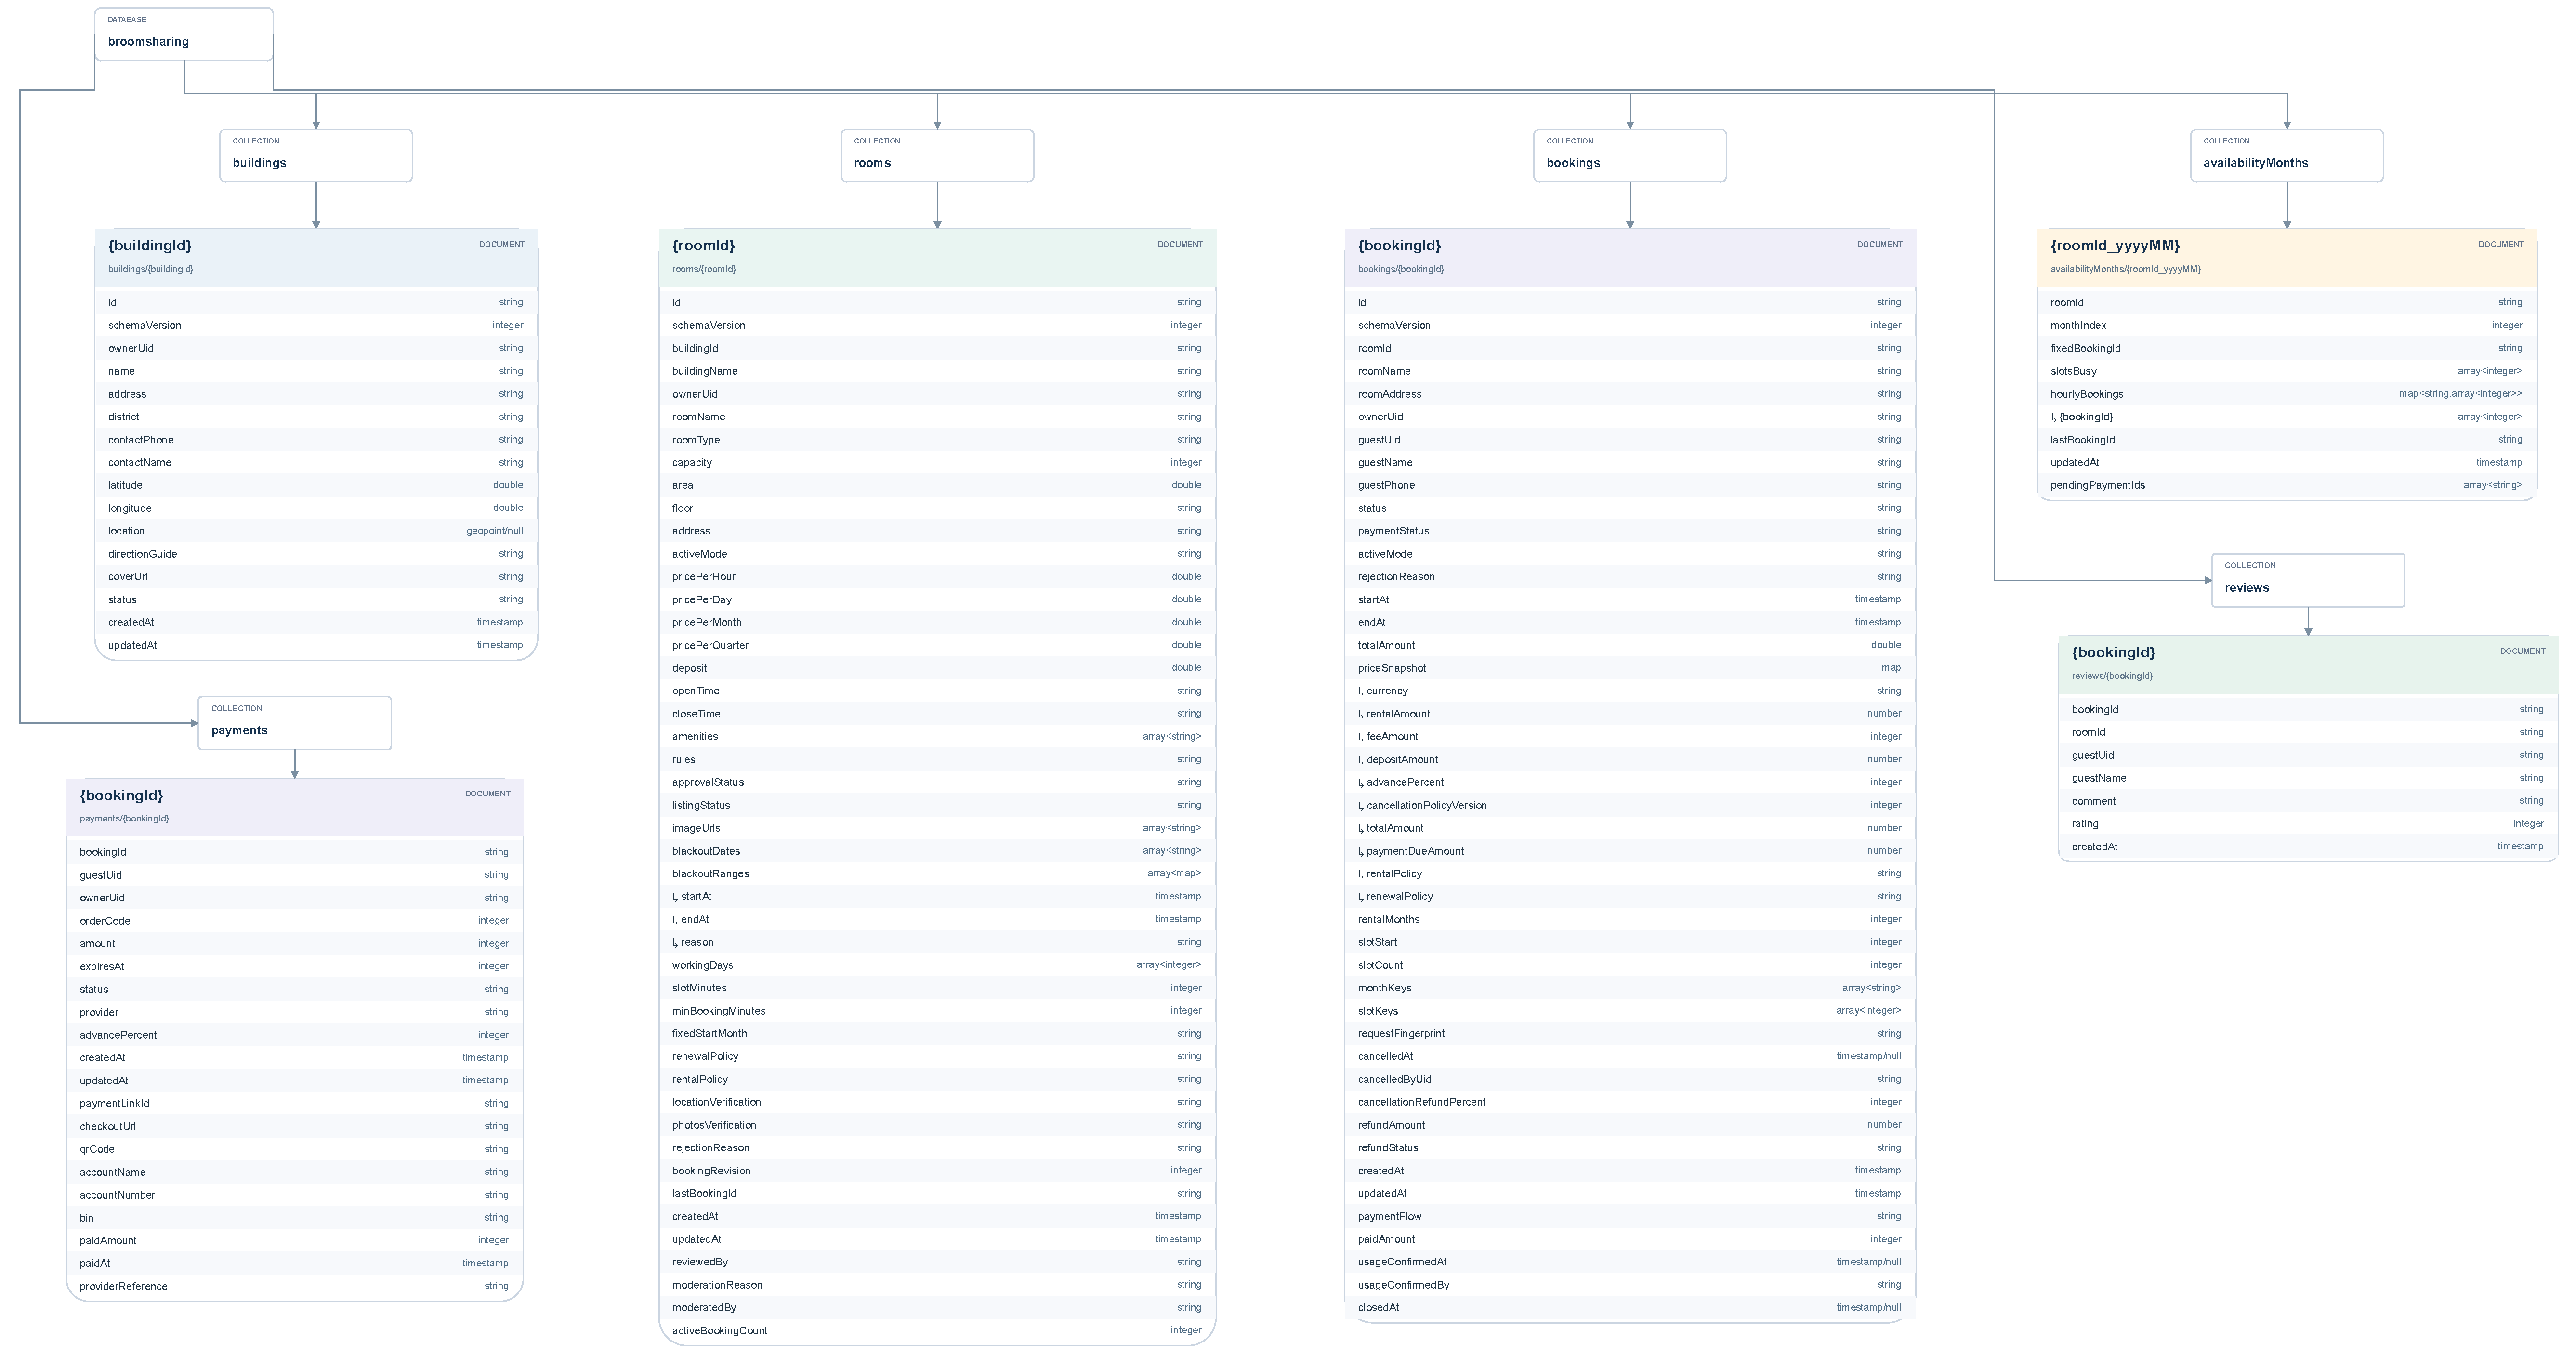
\includegraphics[width=\linewidth,height=0.82\textheight,keepaspectratio]{chapter4/firestore-booking.pdf}
\caption{Cấu trúc tài sản, booking, lịch tháng, thanh toán và đánh giá. Các collection nằm ngang cấp trong database.}
\label{fig:ch4-booking}
\end{figure}
\clearpage
\begin{figure}[p]
\centering
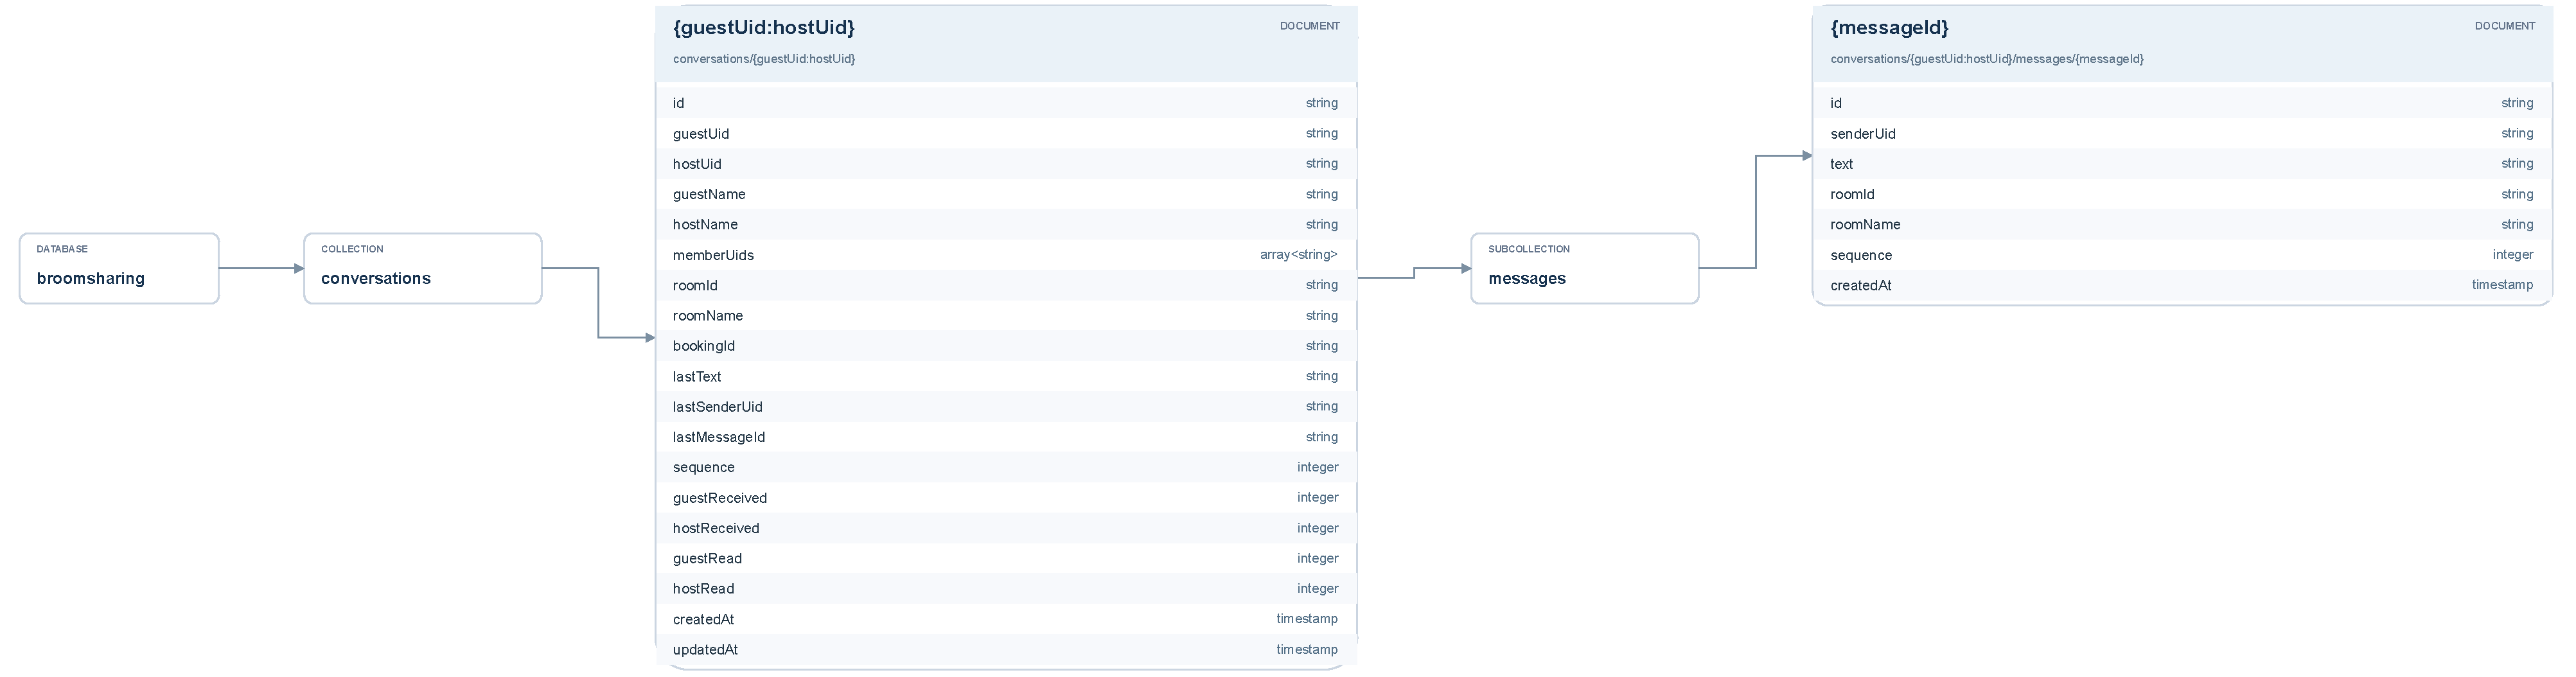
\includegraphics[width=\linewidth,height=0.82\textheight,keepaspectratio]{chapter4/firestore-chat.pdf}
\caption{Cấu trúc hội thoại và subcollection tin nhắn của từng hội thoại.}
\label{fig:ch4-chat}
\end{figure}
\clearpage
\begin{figure}[p]
\centering
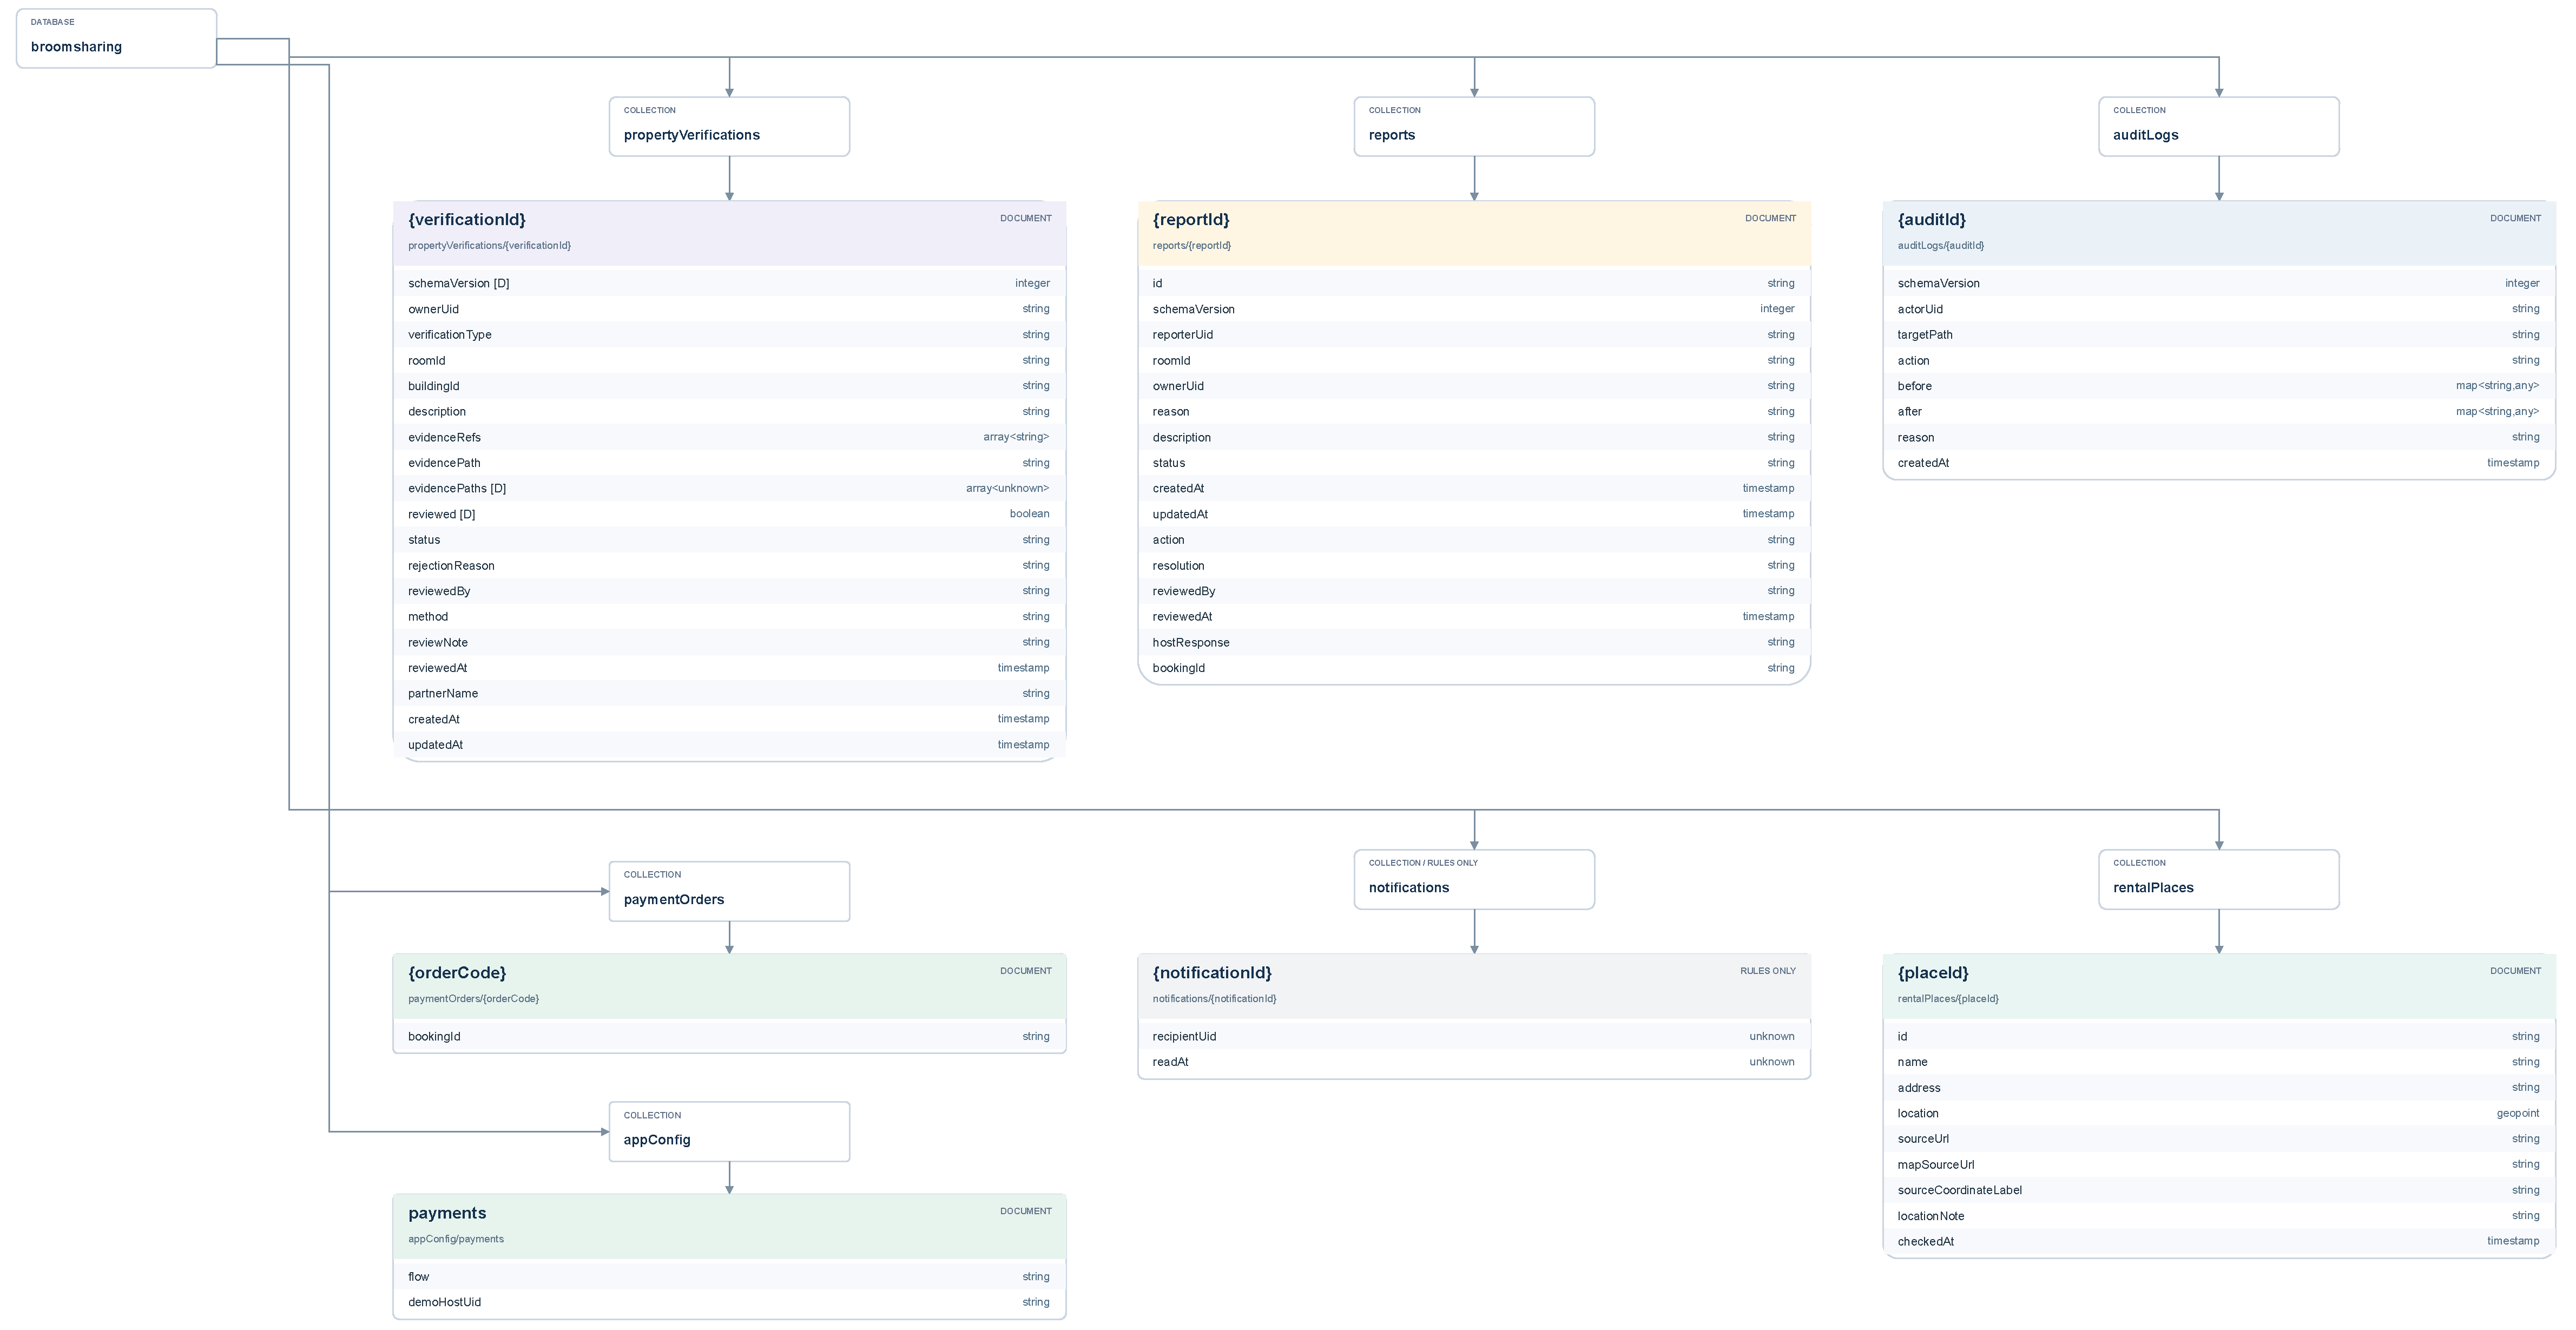
\includegraphics[width=\linewidth,height=0.82\textheight,keepaspectratio]{chapter4/firestore-administration.pdf}
\caption{Nhóm quản trị, dữ liệu tham khảo và cấu hình backend. [D] là trường từ dữ liệu mẫu; Rules-only là contract chưa có luồng ghi hiện tại.}
\label{fig:ch4-administration}
\end{figure}
\clearpage
\BroomLandscapePagefalse
\end{landscape}


Nhóm tài khoản trong Hình~\ref{fig:ch4-accounts} dùng chung UID để liên kết hồ sơ, bản chiếu Host và đơn đăng ký. Nhóm đặt chỗ trong Hình~\ref{fig:ch4-booking} liên kết tài sản với booking và lịch tháng bằng ID. Trong nhóm chat, mỗi document hội thoại sở hữu một subcollection tin nhắn riêng (Hình~\ref{fig:ch4-chat}); dữ liệu xác minh, báo cáo và nhật ký lưu thêm ID hoặc đường dẫn của đối tượng được xử lý (Hình~\ref{fig:ch4-administration}). Các liên kết logic này có ý nghĩa và bội số như Bảng~\ref{tab:ch4-relations-summary}.

\begingroup\small\setstretch{1.08}
\begin{longtable}{@{}>{\raggedright\arraybackslash}p{4.2cm}>{\raggedright\arraybackslash}p{5.15cm}>{\raggedright\arraybackslash}p{5.9cm}@{}}
\caption{Các quan hệ logic chính}\label{tab:ch4-relations-summary}\\
\toprule Nhóm dữ liệu & Liên kết & Ý nghĩa và bội số \\ \midrule\endfirsthead
\toprule Nhóm dữ liệu & Liên kết & Ý nghĩa và bội số \\ \midrule\endhead
\bottomrule\endlastfoot
Tài khoản & UID của hồ sơ, alias và bản chiếu Host. & Một User có một alias theo luồng đăng ký và tối đa một bản chiếu Host; UID liên kết với Authentication. \\
Tài sản & \texttt{rooms.\allowbreak{}building\allowbreak{}Id}; owner UID của Room và Building. & Một Building có nhiều Room; mỗi Room gắn với một Building và Host sở hữu tương ứng. \\
Đặt chỗ & Room ID, guest UID, owner UID. & Mỗi Booking thuộc một Room và hai bên tham gia; một Room có nhiều booking qua thời gian. \\
Lịch tháng & Room ID; fixed booking ID; khóa booking trong \texttt{hourly\allowbreak{}Bookings}. & Mỗi Room có nhiều tháng lịch; một tháng giữ toàn bộ cho một booking cố định hoặc giữ các slot thuê giờ. \\
Yêu thích & Room ID trong nhánh của User. & Quan hệ nhiều với nhiều giữa User và Room thông qua Favorite. \\
Hội thoại & \texttt{member\allowbreak{}Uids}; Room ID, Booking ID; sender UID của message. & Hai thành viên trong một hội thoại; một hội thoại có nhiều message và ngữ cảnh phòng hoặc booking. \\
Quản trị & UID chủ hồ sơ, người báo cáo, người duyệt; Room ID hoặc Building ID. & Hồ sơ xác minh và báo cáo liên kết tới đối tượng được xử lý; liên kết phụ thuộc loại hồ sơ. \\
Thanh toán & Booking ID của Payment; booking ID trong PaymentOrder. & Mỗi booking dùng một Payment cùng ID; order code ánh xạ về booking để đối soát webhook. Payment không phải subcollection của Booking.  \\
Nhật ký & Actor UID và \texttt{target\allowbreak{}Path}. & Actor xác định tài khoản hoặc tiến trình backend; đường dẫn đích thay đổi theo hành động. \\
\end{longtable}\endgroup

Map \texttt{price\allowbreak{}Snapshot} giữ giá và chính sách của booking; mảng \texttt{blackout\allowbreak{}Ranges} chứa các khoảng khóa lịch; map \texttt{hourly\allowbreak{}Bookings} ánh xạ booking ID tới tập slot. Đây là dữ liệu nhúng trong document. Room được thuê độc quyền trong khoảng $[startAt,endAt)$: PENDING giữ lịch tạm chờ thanh toán trong tối đa 5 phút, HOURLY dùng slot 30 phút và FIXED giữ trọn một hoặc ba tháng. Mảng \texttt{pending\allowbreak{}Payment\allowbreak{}Ids} phân biệt các khóa tạm chờ thanh toán với lịch đã xác nhận. Transaction duy trì sự nhất quán giữa booking, lịch tháng và revision của phòng.

\subsection{Một số thao tác dữ liệu tiêu biểu}
\label{sec:ch4-operations}

\subsubsection{Các nhóm thao tác dữ liệu}

Các Repository thực hiện ba nhóm thao tác: đọc dữ liệu theo điều kiện, theo dõi thay đổi bằng listener và ghi dữ liệu nghiệp vụ. Truy vấn danh sách giới hạn phạm vi theo trạng thái hoặc UID; listener cập nhật booking và trao đổi giữa hai bên; transaction xử lý những thay đổi liên quan nhiều document. Bảng~\ref{tab:ch4-operations} tổng hợp các thao tác tiêu biểu và dữ liệu tham gia.

\begingroup\small\setstretch{1.08}
\begin{longtable}{@{}>{\raggedright\arraybackslash}p{3.45cm}>{\raggedright\arraybackslash}p{4.25cm}>{\raggedright\arraybackslash}p{7.55cm}@{}}
\caption{Các thao tác dữ liệu tiêu biểu trong ứng dụng}\label{tab:ch4-operations}\\
\toprule Thao tác & Dữ liệu & Cách xử lý trong Repository \\ \midrule\endfirsthead
\toprule Thao tác & Dữ liệu & Cách xử lý trong Repository \\ \midrule\endhead
\midrule\multicolumn{3}{r}{\small Còn tiếp ở trang sau}\\\endfoot
\bottomrule\endlastfoot
Tải danh sách phòng & \texttt{rooms}; bổ sung Building và PublicHost. & Lọc APPROVED, ACTIVE; sắp theo document ID, lấy tối đa 20 phòng và phân trang bằng con trỏ. \\
Theo dõi booking & \texttt{bookings}. & Lọc \texttt{guest\allowbreak{}Uid} hoặc \texttt{owner\allowbreak{}Uid} theo tài khoản; nhận thay đổi qua listener. \\
Đọc lịch phòng & \texttt{availability\allowbreak{}Months}. & Đọc các document tháng liên quan để xác định lịch giữ chỗ theo giờ hoặc theo tháng. \\
Tạo booking & Booking, lịch tháng, Room và AuditLog. & Đọc và kiểm tra trong transaction; ghi booking PENDING cùng khóa lịch, revision phòng và nhật ký. \\
Chuyển trạng thái booking & Booking, lịch tháng, Room và AuditLog. & Kiểm tra bên thực hiện, trạng thái và thời gian; hủy, hết hạn hoặc khép lượt giải phóng khóa lịch tương ứng; booking mới được backend xác nhận sau thanh toán. \\
Đối soát thanh toán & Payment, Booking, lịch tháng, Room và AuditLog. & Backend kiểm tra kết quả payOS; xác nhận khi nhận đủ tiền đúng hạn hoặc khép link chưa trả và nhả lịch, không tự hoàn tiền.  \\
Theo dõi chat & \texttt{conversations} và subcollection \texttt{messages}. & Inbox lọc UID trong \texttt{member\allowbreak{}Uids}; tin nhắn sắp theo \texttt{sequence}, giới hạn số lượng và nhận cập nhật qua listener. \\
Gửi tin nhắn & Message và document hội thoại cha. & Transaction ghi tin, cập nhật preview, thứ tự và bộ đếm nhận tin của bên còn lại. \\
Lưu phòng yêu thích & \texttt{users/\allowbreak{}\{uid\}/\allowbreak{}favorites/\allowbreak{}\{room\allowbreak{}Id\}}. & Ghi ID, tên phòng và thời điểm lưu; bỏ yêu thích bằng cách xóa document tại cùng đường dẫn. \\
\end{longtable}\endgroup

Thao tác đọc danh sách và theo dõi thay đổi phục vụ hai nhu cầu khác nhau. Danh sách phòng được tải theo từng trang, còn booking và chat cần phản ánh cập nhật trong quá trình sử dụng. Các listener này bỏ qua snapshot từ cache hoặc còn ghi đang chờ xác nhận, thông qua metadata \texttt{isFrom\allowbreak{}Cache()} và \texttt{hasPending\allowbreak{}Writes()} \parencite{firebase_listeners}.


\subsubsection{Các truy vấn tiêu biểu}
\texttt{RoomRepository.page()} lọc phòng APPROVED, ACTIVE và phân trang theo document ID. Mỗi lượt lấy tối đa 20 document; \texttt{after} là ID cuối của lượt trước, còn lượt đầu bằng \texttt{null}. Con trỏ tránh đọc lại phần đã tải \parencite{firebase_queries,firebase_query_cursors}.

\par\medskip\noindent\begin{minipage}{\linewidth}
\inputminted[firstnumber=1]{java}{Resources/chapter4/code/room-query.java}
\end{minipage}\par\medskip

Repository đọc từ máy chủ, bổ sung Building và PublicHost để tạo RoomListing. RoomViewModel ghép kết quả theo Room ID, giữ con trỏ và phát LiveData cho MainActivity. Với tìm kiếm hoặc bộ lọc, các trang còn lại được tải trước khi kết luận không có kết quả; cờ \texttt{hasMore} chỉ cho phép thử trang tiếp theo, không bảo đảm trang đó còn dữ liệu.

\texttt{BookingRepository.watchMine()} dùng truy vấn theo UID người thuê. Document được ánh xạ sang Booking và sắp theo thời điểm tạo giảm dần; BookingViewModel chuyển kết quả thành trạng thái để MyBookingsActivity hiển thị. Listener được gỡ khi màn hình dừng, tránh tiếp tục theo dõi dữ liệu không còn được sử dụng.

\par\medskip\noindent\begin{minipage}{\linewidth}
\inputminted[firstnumber=1]{java}{Resources/chapter4/code/booking-query-listener.java}
\end{minipage}\par\medskip

Kết quả truy vấn rỗng được phân biệt với lỗi kết nối. Khi mất mạng, các màn đọc phòng và lịch sử đặt chỗ sử dụng bản sao SQLite có ghi thời điểm lưu; bản sao này không được dùng để xác nhận lịch trống hoặc thanh toán.

\subsubsection{Tạo booking bằng transaction}
\texttt{BookingRepository.create()} thực hiện các bước tại Bảng~\ref{tab:ch4-transaction}. Booking ID được băm từ UID và request key; fingerprint kiểm tra nội dung yêu cầu. Cùng ID và fingerprint trả lại booking đã tạo, còn khác nội dung bị từ chối để tránh tái sử dụng sai mã gửi.

\begin{table}[H]\centering\small
\caption{Các bước tạo booking trong transaction}\label{tab:ch4-transaction}
\begin{tabularx}{\linewidth}{@{}p{2.7cm}X@{}}\toprule
Bước & Dữ liệu và điều kiện\\\midrule
Đọc & User, Room, PublicHost, Building, cấu hình \texttt{appConfig/payments} và các tháng lịch liên quan.\\
Kiểm tra & Tài khoản, Host và tài sản còn hợp lệ; Room APPROVED, ACTIVE, cùng chủ Building và khác người thuê. Booking thuộc kênh demo INSTANT\_5M.\\
Tính giá, giữ lịch & BookingPolicy tính lại kỳ thuê, giá từ Room. Thuê giờ kiểm tra slot không giao \texttt{slotsBusy}; thuê cố định yêu cầu các tháng chưa bị giữ.\\
Ghi đồng thời & Booking PENDING, khóa lịch tạm, revision phòng và AuditLog. Lỗi ở một bước làm toàn bộ giao dịch không được chấp nhận.\\
\bottomrule\end{tabularx}
\end{table}

Firestore có thể chạy lại callback khi document đã đọc thay đổi đồng thời \parencite{firebase_transaction}. Hai yêu cầu trùng lịch vì vậy phải kiểm tra lại trên cùng lịch tháng trước khi ghi. Kết quả transaction chỉ là giữ chỗ chờ thanh toán; ứng dụng mở QR ngay, chưa báo đã đặt thành công.

Booking mới lưu \texttt{schemaVersion=2}, \texttt{priceSnapshot} và \texttt{paymentFlow=INSTANT\_5M}. Backend xác minh kết quả payOS trước khi chuyển PAID/CONFIRMED. Hết hạn chưa trả chuyển EXPIRED và nhả đúng khóa lịch; tiền đến muộn, sai số tiền hoặc lịch không hợp lệ chuyển REVIEW\_REQUIRED để đối soát thủ công.

\Needspace{8\baselineskip}
\subsection{Phân quyền và bảo vệ dữ liệu}
\label{sec:ch4-security}

Firestore Rules kết hợp UID, vai trò, trạng thái ACTIVE và quyền sở hữu để kiểm soát truy cập. Guest và Host đều có quyền thuê, nhưng không được tự đặt phòng của mình. Bảng~\ref{tab:ch4-permissions} tóm tắt các nhóm quyền chính; các thao tác ngoài nhánh được cho phép chịu quy tắc từ chối mặc định.

\begingroup\small\setstretch{1.08}
\begin{longtable}{@{}>{\raggedright\arraybackslash}p{4.1cm}>{\raggedright\arraybackslash}p{11.15cm}@{}}
\caption{Phân quyền theo nhóm dữ liệu}\label{tab:ch4-permissions}\\
\toprule Nhóm & Quyền truy cập chính \\ \midrule\endfirsthead
\toprule Nhóm & Quyền truy cập chính \\ \midrule\endhead
\bottomrule\endlastfoot
Hồ sơ và đơn Host & Chủ hồ sơ hoặc Admin được đọc. Người dùng sửa nhóm trường hồ sơ cho phép; Guest nộp đơn, Admin xét duyệt. PublicHost được đọc bởi tài khoản hoạt động. \\
Alias và dữ liệu cá nhân & \texttt{usernames} cho phép get trước đăng nhập, list chỉ dành cho Admin. Favorite và mốc đã đọc thuộc quyền tài khoản sở hữu nhánh dữ liệu. \\
Tòa nhà và phòng & Host quản lý tài sản của mình; Admin được cập nhật Room, không có nhánh ghi Building riêng. Phòng công khai cho tài khoản hoạt động khi APPROVED và ACTIVE. \\
Booking và lịch & Hai bên tham gia và Admin được đọc Booking. Chuyển trạng thái phụ thuộc vai trò, thời gian và lịch; Admin không có nhánh chuyển tùy ý. Ghi lịch phải khớp booking trong cùng thao tác. \\
Thanh toán và cấu hình & Người thuê, Host liên quan và Admin được đọc Payment; client không được tự ghi trạng thái tiền. PaymentOrder chỉ do backend truy cập; cấu hình kênh cho tài khoản hoạt động đọc, không chứa khóa payOS.  \\
Chat & Chỉ thành viên đang hoạt động đọc hội thoại và message. Gửi tin cập nhật đồng thời preview, thứ tự và bộ đếm; mỗi bên chỉ tăng mốc đã đọc của mình. Admin không có quyền đọc riêng. \\
Quản trị và tham khảo & Chủ hồ sơ hoặc Admin đọc xác minh; Admin cập nhật kết quả. Báo cáo được đọc theo người gửi, Host liên quan hoặc Admin. Audit chỉ Admin đọc; RentalPlace chỉ cho tài khoản hoạt động đọc. \\
\end{longtable}\endgroup

Quyền ghi còn phụ thuộc nội dung và tính nhất quán giữa document. Rules dùng danh sách trường cho phép và \texttt{diff().\allowbreak{}affected\allowbreak{}Keys()} để giới hạn thay đổi; \texttt{get\allowbreak{}After()} kiểm tra trạng thái sau ghi của các document liên quan \parencite{firebase_rules_fields,firebase_rules_conditions}. Hàm \texttt{held\allowbreak{}Month()} đối chiếu booking với lịch tháng trước khi chấp nhận thao tác giữ chỗ; client không được ghi booking và lịch rời nhau.

Backend dùng Firebase Admin SDK nên phải tự xác thực Firebase ID token, kiểm tra người tham gia và đối chiếu kết quả payOS; không dựa vào Rules để xác thực lệnh ghi của server \parencite{firebase_rules_conditions}. Khóa dịch vụ được giữ ở môi trường backend. Ảnh và minh chứng DEMO hiện dùng URL Cloudinary; Rules kiểm tra đường dẫn theo UID và đối tượng liên quan. Ảnh giấy tờ DEMO công khai theo URL không được xem là cơ chế bảo vệ giấy tờ cá nhân thật.

\endgroup

\chapstart
\section{XÂY DỰNG ỨNG DỤNG VÀ THIẾT KẾ KIẾN TRÚC}
\label{sec:application-build}
\begingroup
\setlist[itemize]{leftmargin=1.27cm,label=\textbullet,itemsep=2pt,topsep=4pt}
\setlist[enumerate]{leftmargin=1.27cm,itemsep=2pt,topsep=4pt}
\setlength{\emergencystretch}{1em}
\widowpenalty=10000
\clubpenalty=10000
\subsection{Tổng quan kiến trúc ứng dụng}
\label{sec:implemented-architecture}

\subsubsection{Tổ chức ứng dụng theo MVVM, Repository và Model}
BroomSharing sử dụng Java và XML theo mô hình MVVM + Repository + Model. XML định nghĩa bố cục; Activity và Adapter hiển thị dữ liệu, tiếp nhận thao tác. ViewModel giữ trạng thái màn hình qua LiveData, Repository truy cập Firestore và các dịch vụ mạng, còn Model biểu diễn các đối tượng như Room và Booking. Cách phân chia này tách giao diện khỏi xử lý dữ liệu \parencite{android_views,android_data,broomsharing_source}.

Hình~\ref{fig:mvvm} thể hiện luồng tương tác giữa các thành phần và dịch vụ ngoài. Authentication quản lý danh tính, Firestore lưu nghiệp vụ, Cloudinary lưu ảnh; bản đồ kết hợp MapLibre, MapTiler và openrouteservice. Backend Java kết nối payOS để tạo và đối soát giao dịch. Biểu tượng trong hình sử dụng bộ Fluent UI System Icons \parencite{fluent_system_icons}.

\begin{figure}[H]
\centering
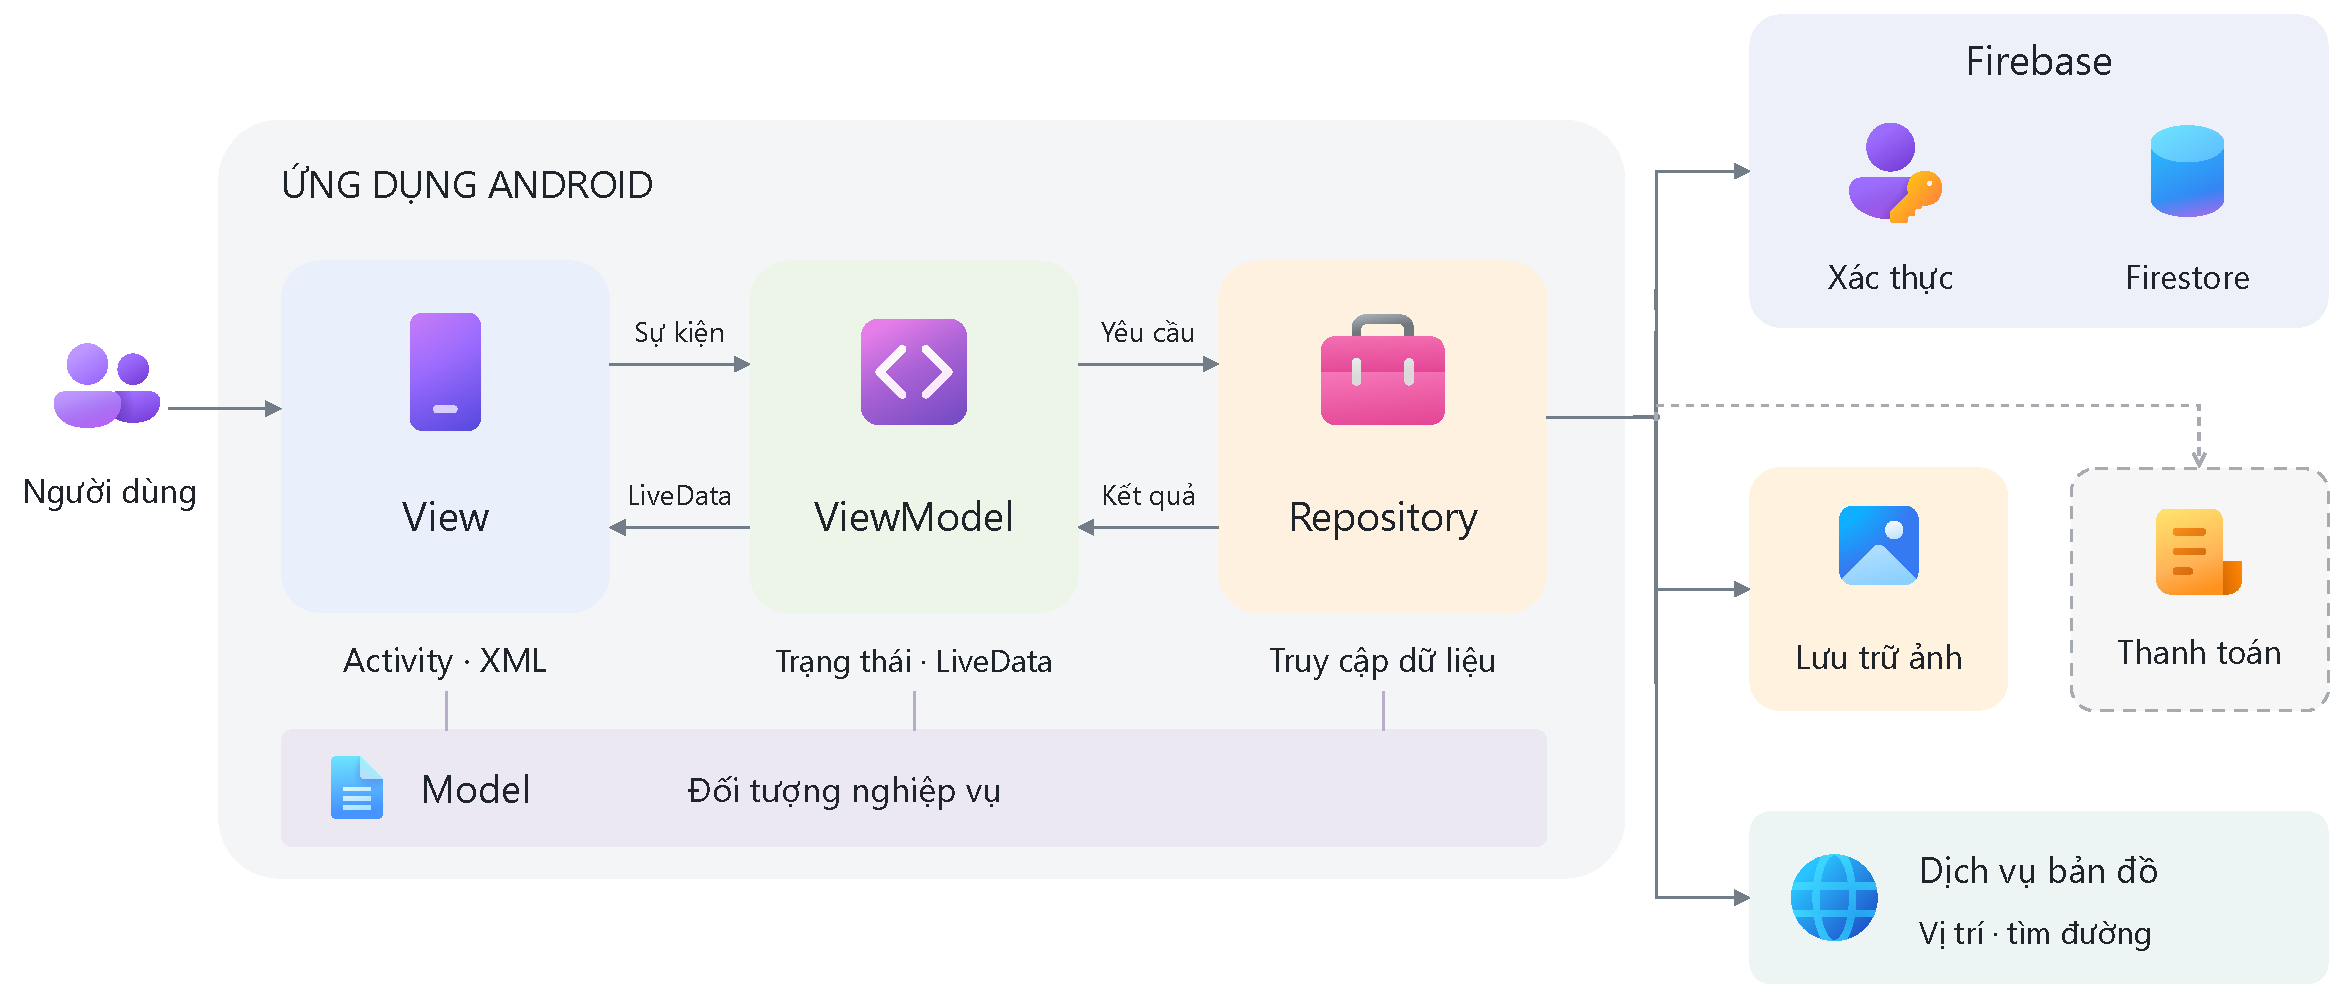
\includegraphics[width=\linewidth]{chapter5/application-architecture.pdf}
\caption{Kiến trúc tổng quan của ứng dụng BroomSharing}
\label{fig:mvvm}
\end{figure}

\subsubsection{Luồng xử lý giữa giao diện và các nguồn dữ liệu}
Activity gửi thao tác tới ViewModel; ViewModel gọi Repository rồi phát trạng thái tải, dữ liệu hoặc lỗi qua LiveData. Chẳng hạn, khi Admin chọn hàng đợi, Repository đọc nhóm hồ sơ tương ứng; khi xét duyệt, dữ liệu được kiểm tra lại trước khi ghi và giao diện chặn gửi lặp trong lúc chờ kết quả.

Với booking, transaction cập nhật đồng thời lượt thuê, lịch và dữ liệu kiểm soát liên quan \parencite{firebase_transaction}. Trạng thái tiền do backend đối soát rồi chuyển tới giao diện qua listener; mở QR hoặc quay về ứng dụng không được xem là đã thanh toán.

\subsection{Kết nối Firebase và các dịch vụ hỗ trợ}
\label{sec:firebase-and-services}

\subsubsection{Kết nối Firebase Authentication và Cloud Firestore}
Ứng dụng kết nối Firebase qua \texttt{google-services.json} và plugin Google Services; Firebase BoM quản lý phiên bản SDK \parencite{firebase_android}. FirebaseHelper chọn database \texttt{broomsharing} và cung cấp đối tượng Firestore dùng chung cho các Repository.

FirebaseAuthRepository xác thực tài khoản và gửi email đặt lại mật khẩu bằng \texttt{sendPasswordResetEmail()} \parencite{firebase_auth_users}. UID liên kết hồ sơ \texttt{users/\{uid\}}; SessionActivity điều hướng theo vai trò và trạng thái, Security Rules kiểm soát request Android. Backend xác minh ID token bằng Admin SDK và kiểm tra quyền trên booking \parencite{firebase_admin_token}.

\subsubsection{Tích hợp các dịch vụ và thư viện hỗ trợ}
Bảng~\ref{tab:implemented-services} phân biệt các dịch vụ dữ liệu với thư viện hiển thị bản đồ. Client xử lý phản hồi trước khi cập nhật giao diện.

\begin{table}[htbp]
\centering\small
\caption{Các thành phần kết nối dữ liệu và hiển thị bản đồ}
\label{tab:implemented-services}
\begin{tabularx}{\linewidth}{@{}p{4.1cm}X@{}}
\toprule
Thành phần & Vai trò trong ứng dụng \\
\midrule
Firebase Authentication & Xác thực, quản lý phiên và gửi liên kết đặt lại mật khẩu. \\
Cloud Firestore & Lưu hồ sơ và dữ liệu nghiệp vụ; truy vấn, listener và transaction. \\
MapLibre Native & Thư viện dựng bản đồ, marker và tuyến trên Android. \\
MapTiler & Cung cấp nền bản đồ, geocoding và địa điểm lân cận. \\
openrouteservice & Trả GeoJSON tuyến ô tô, chiều dài và thời gian ước tính. \\
Cloudinary & Nhận ảnh, tệp DEMO và trả URL HTTPS cùng metadata. \\
Backend Java và payOS & Tạo QR, nhận webhook và đối soát tiền theo booking. \\
\bottomrule
\end{tabularx}
\end{table}

Tuyến đường trả về chỉ có thời gian ước tính, không có giao thông trực tiếp \parencite{maplibre_android,maptiler_geocoding,ors_directions}. Cloudinary dùng unsigned upload; Firestore ghi URL sau khi tải thành công. RemoteImageClient kiểm tra ảnh lấy từ URL \parencite{cloudinary_unsigned}.

OkHttp gửi request, JSONObject đọc JSON; Picasso và Glide hiển thị ảnh. Android gửi booking ID và ID token tới backend Java; webhook payOS chuyển qua WEB\_TCC để đối soát và cập nhật Firestore. Khóa merchant ở backend; worker chỉ quét khi có việc, còn bộ đếm chạy tại thiết bị \parencite{payos_java,payos_webhook,firebase_listeners}. Kênh demo phục vụ một Host, chưa hoàn tiền qua API; quy trình tại Mục~\ref{sec:execution-booking-payment}.

SQLite lưu bản sao phòng và booking để đọc ngoại tuyến. OfflineRepository phối hợp nguồn dữ liệu cục bộ này với các màn đọc; cơ chế lưu và phục hồi được trình bày tại Mục~\ref{sec:sqlite-offline}.

\subsection{Xây dựng các màn hình chức năng}
\label{sec:application-screens}
\subsubsection{Đăng ký, đăng nhập và quản lý hồ sơ}
\label{sec:screen-account}
Biểu mẫu tài khoản kiểm tra thông tin bắt buộc, email, số điện thoại và mật khẩu trước khi gửi. AuthViewModel giữ trạng thái xử lý; FirebaseAuthRepository xác thực bằng email hoặc tra cứu username trong \texttt{usernames}. UID đăng nhập liên kết với hồ sơ \texttt{users}; vai trò và trạng thái quyết định khu vực được mở, không lấy trực tiếp từ dữ liệu người dùng tự nhập \parencite{broomsharing_source}.

Hình~\ref{fig:actual-account} minh họa màn đăng nhập và hồ sơ hiện thực. Chức năng quên mật khẩu gửi liên kết qua Firebase Authentication. Hồ sơ cho phép chọn ảnh từ thư viện hoặc nhập URL; ảnh được kiểm tra, tải lên Cloudinary rồi cập nhật \texttt{photoUrl}. Với Host, ảnh và bản chiếu \texttt{publicHosts} được đồng bộ trong transaction. Ảnh hồ sơ được tải bằng Picasso; cập nhật ảnh không cho phép sửa vai trò hoặc trạng thái tài khoản.

\begin{figure}[H]\centering
\begin{minipage}[t]{0.34\linewidth}\centering
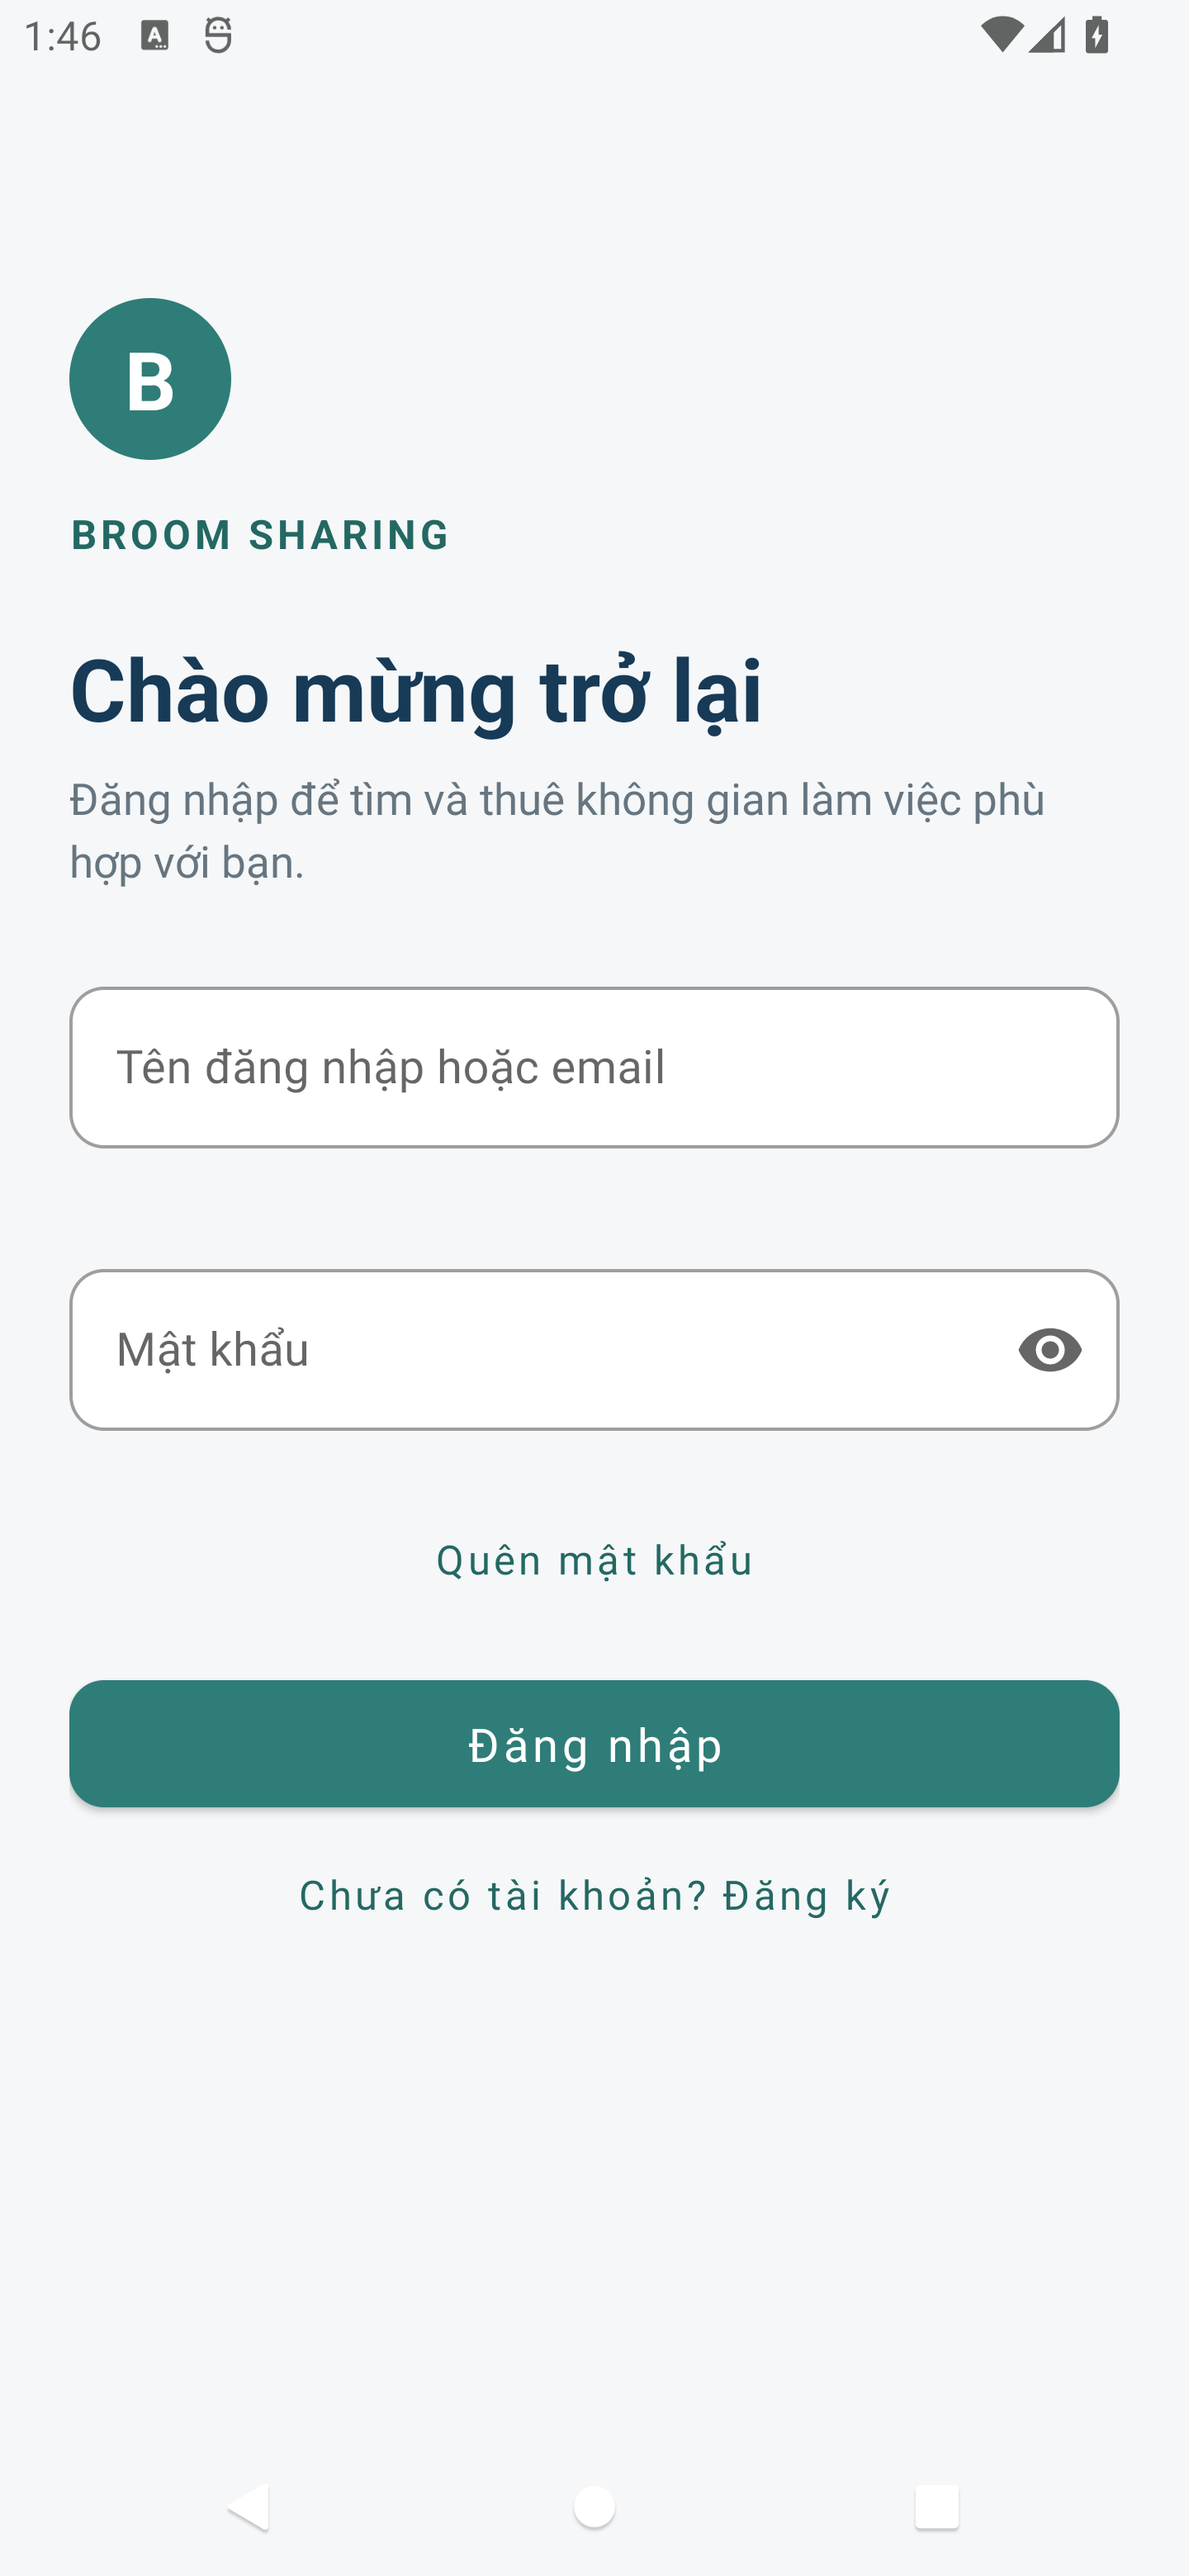
\includegraphics[width=\linewidth]{chapter5/final/login.png}\\[-1mm]
{\small (a) Đăng nhập}
\end{minipage}\hspace{0.05\linewidth}%
\begin{minipage}[t]{0.34\linewidth}\centering
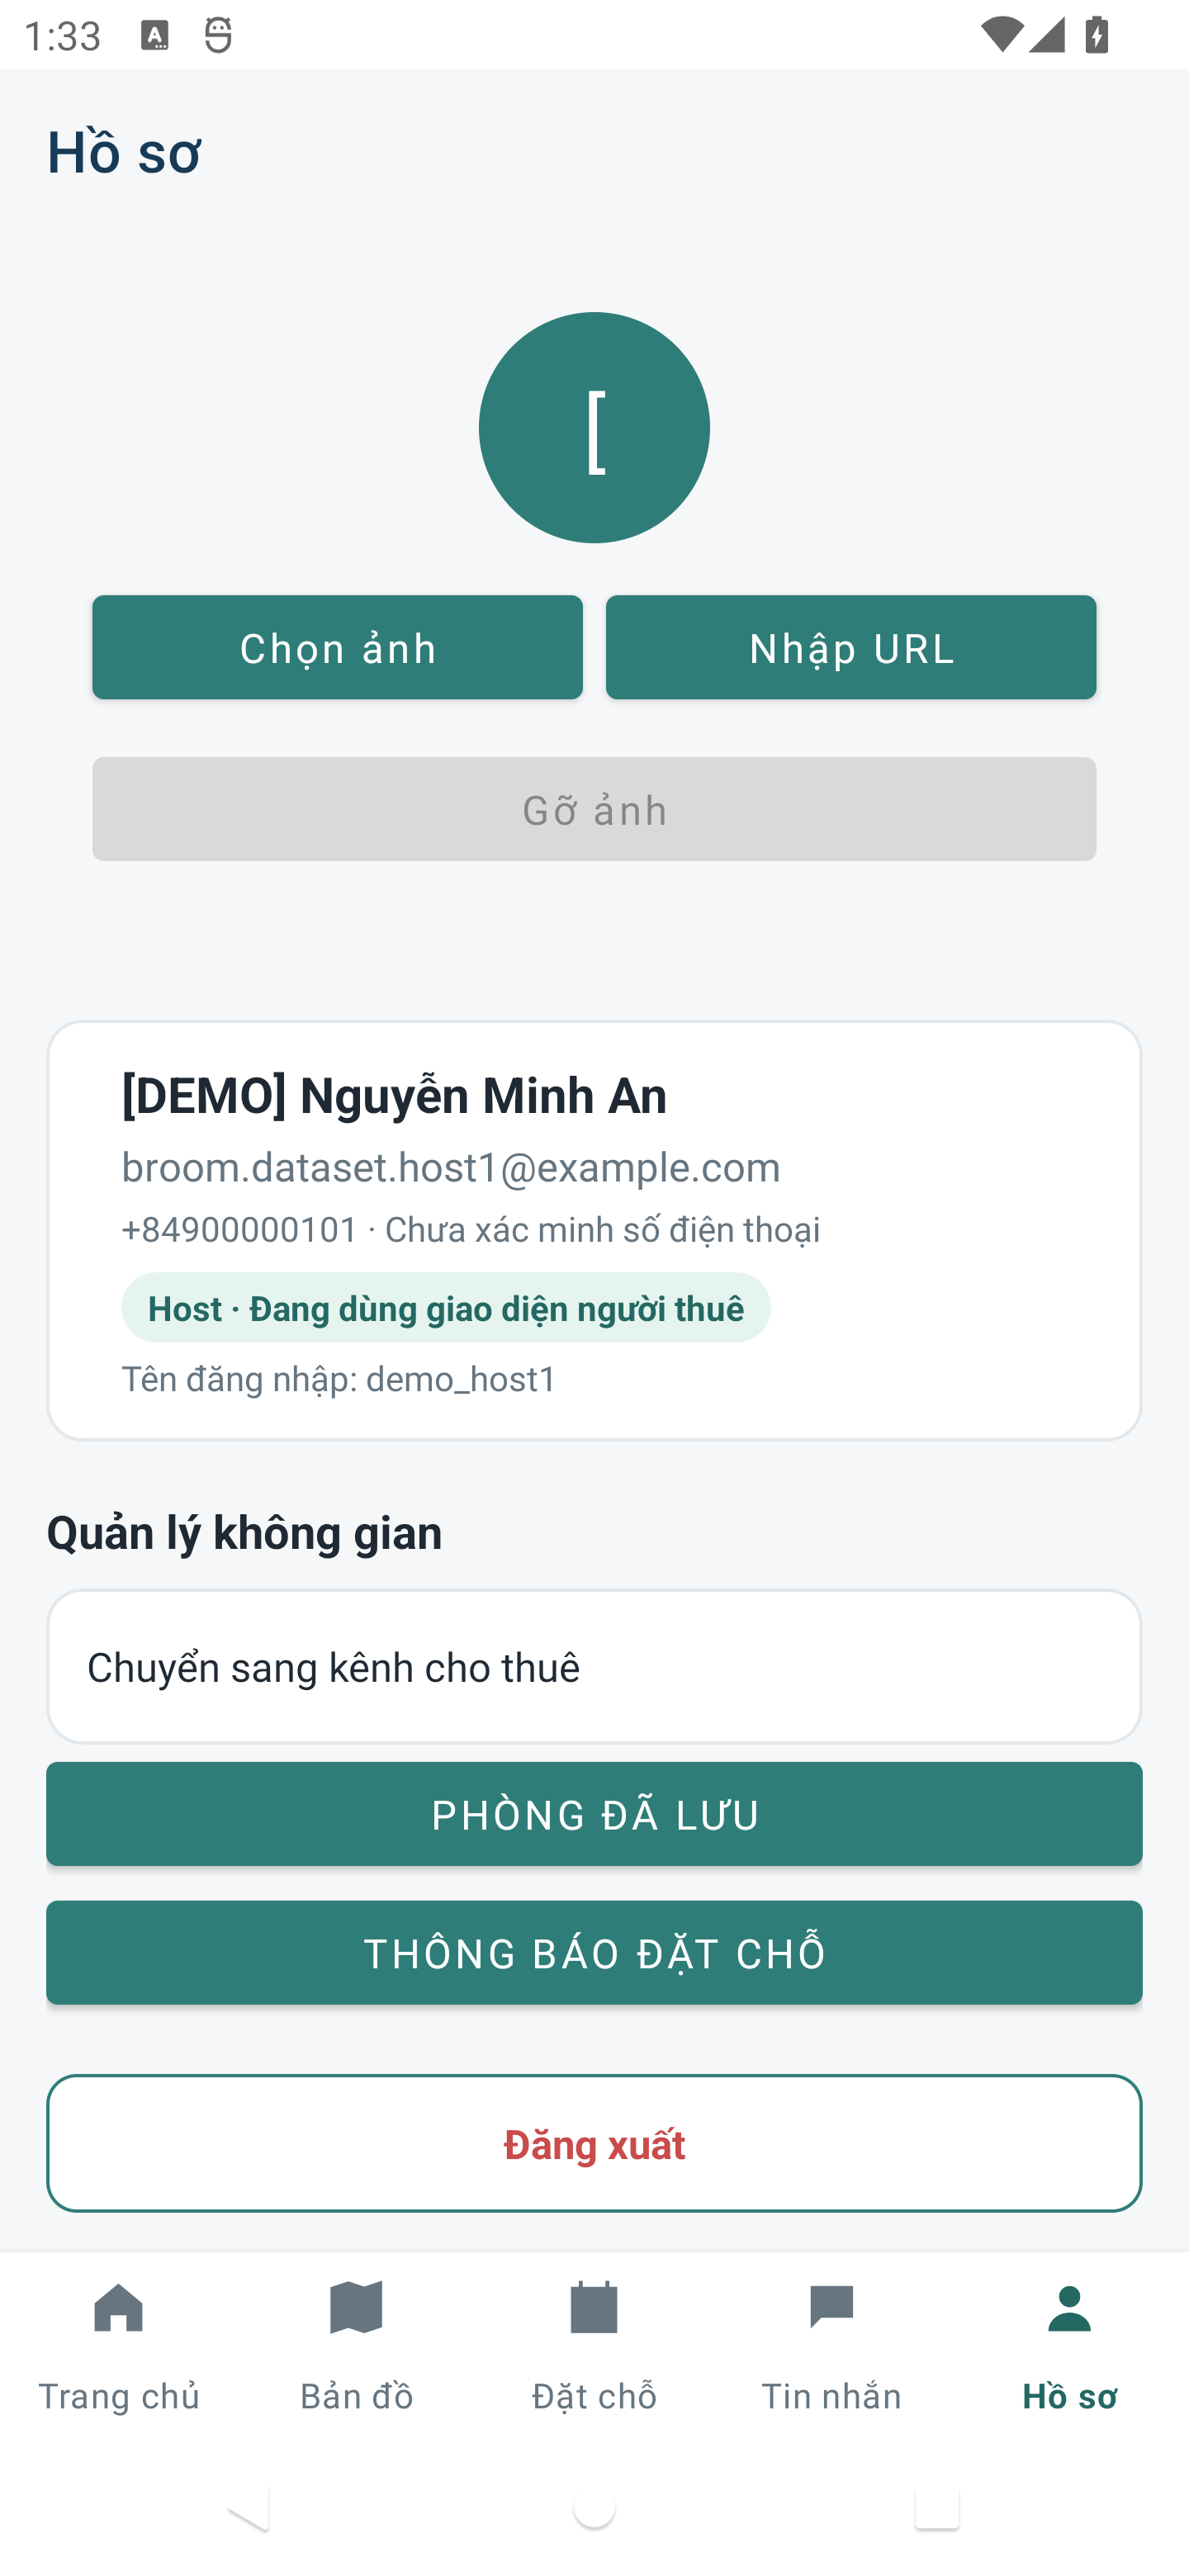
\includegraphics[width=\linewidth]{chapter5/final/profile.png}\\[-1mm]
{\small (b) Hồ sơ và ảnh đại diện}
\end{minipage}
\caption{Giao diện xác thực và hồ sơ tài khoản}
\label{fig:actual-account}
\end{figure}

\subsubsection{Trang chủ, tìm kiếm và chi tiết không gian}
\label{sec:screen-discovery}
Trang chủ tải phòng đã duyệt, đang hoạt động theo từng trang 20 document. RoomRepository bổ sung thông tin Building và PublicHost để tạo RoomListing; RoomViewModel ghép theo Room ID và giữ con trỏ tải tiếp. Từ khóa và bộ lọc khu vực, loại phòng, chế độ thuê, sức chứa, giá được áp dụng trên dữ liệu đã tải; khi cần, ứng dụng tải tiếp trước khi kết luận không có kết quả.

Hình~\ref{fig:actual-discovery} cho thấy thẻ phòng và trang chi tiết cùng đối tượng. Chi tiết hiển thị ảnh, đơn vị giá, tiện ích, lịch hoạt động và chính sách; các nút lưu, liên hệ và đặt chỗ giữ nguyên Room ID. FavoritesRepository ghi hoặc xóa document \texttt{users/\{uid\}/favorites/\{roomId\}}. Với phòng tháng/quý, nhãn lịch được dựng từ lịch tháng, phân biệt kỳ trống, tạm giữ, đặt trước và kỳ thuê còn tối đa ba ngày; nhãn không thay cho bước kiểm tra kỳ thuê cụ thể.

\begin{figure}[H]\centering
\begin{minipage}[t]{0.34\linewidth}\centering
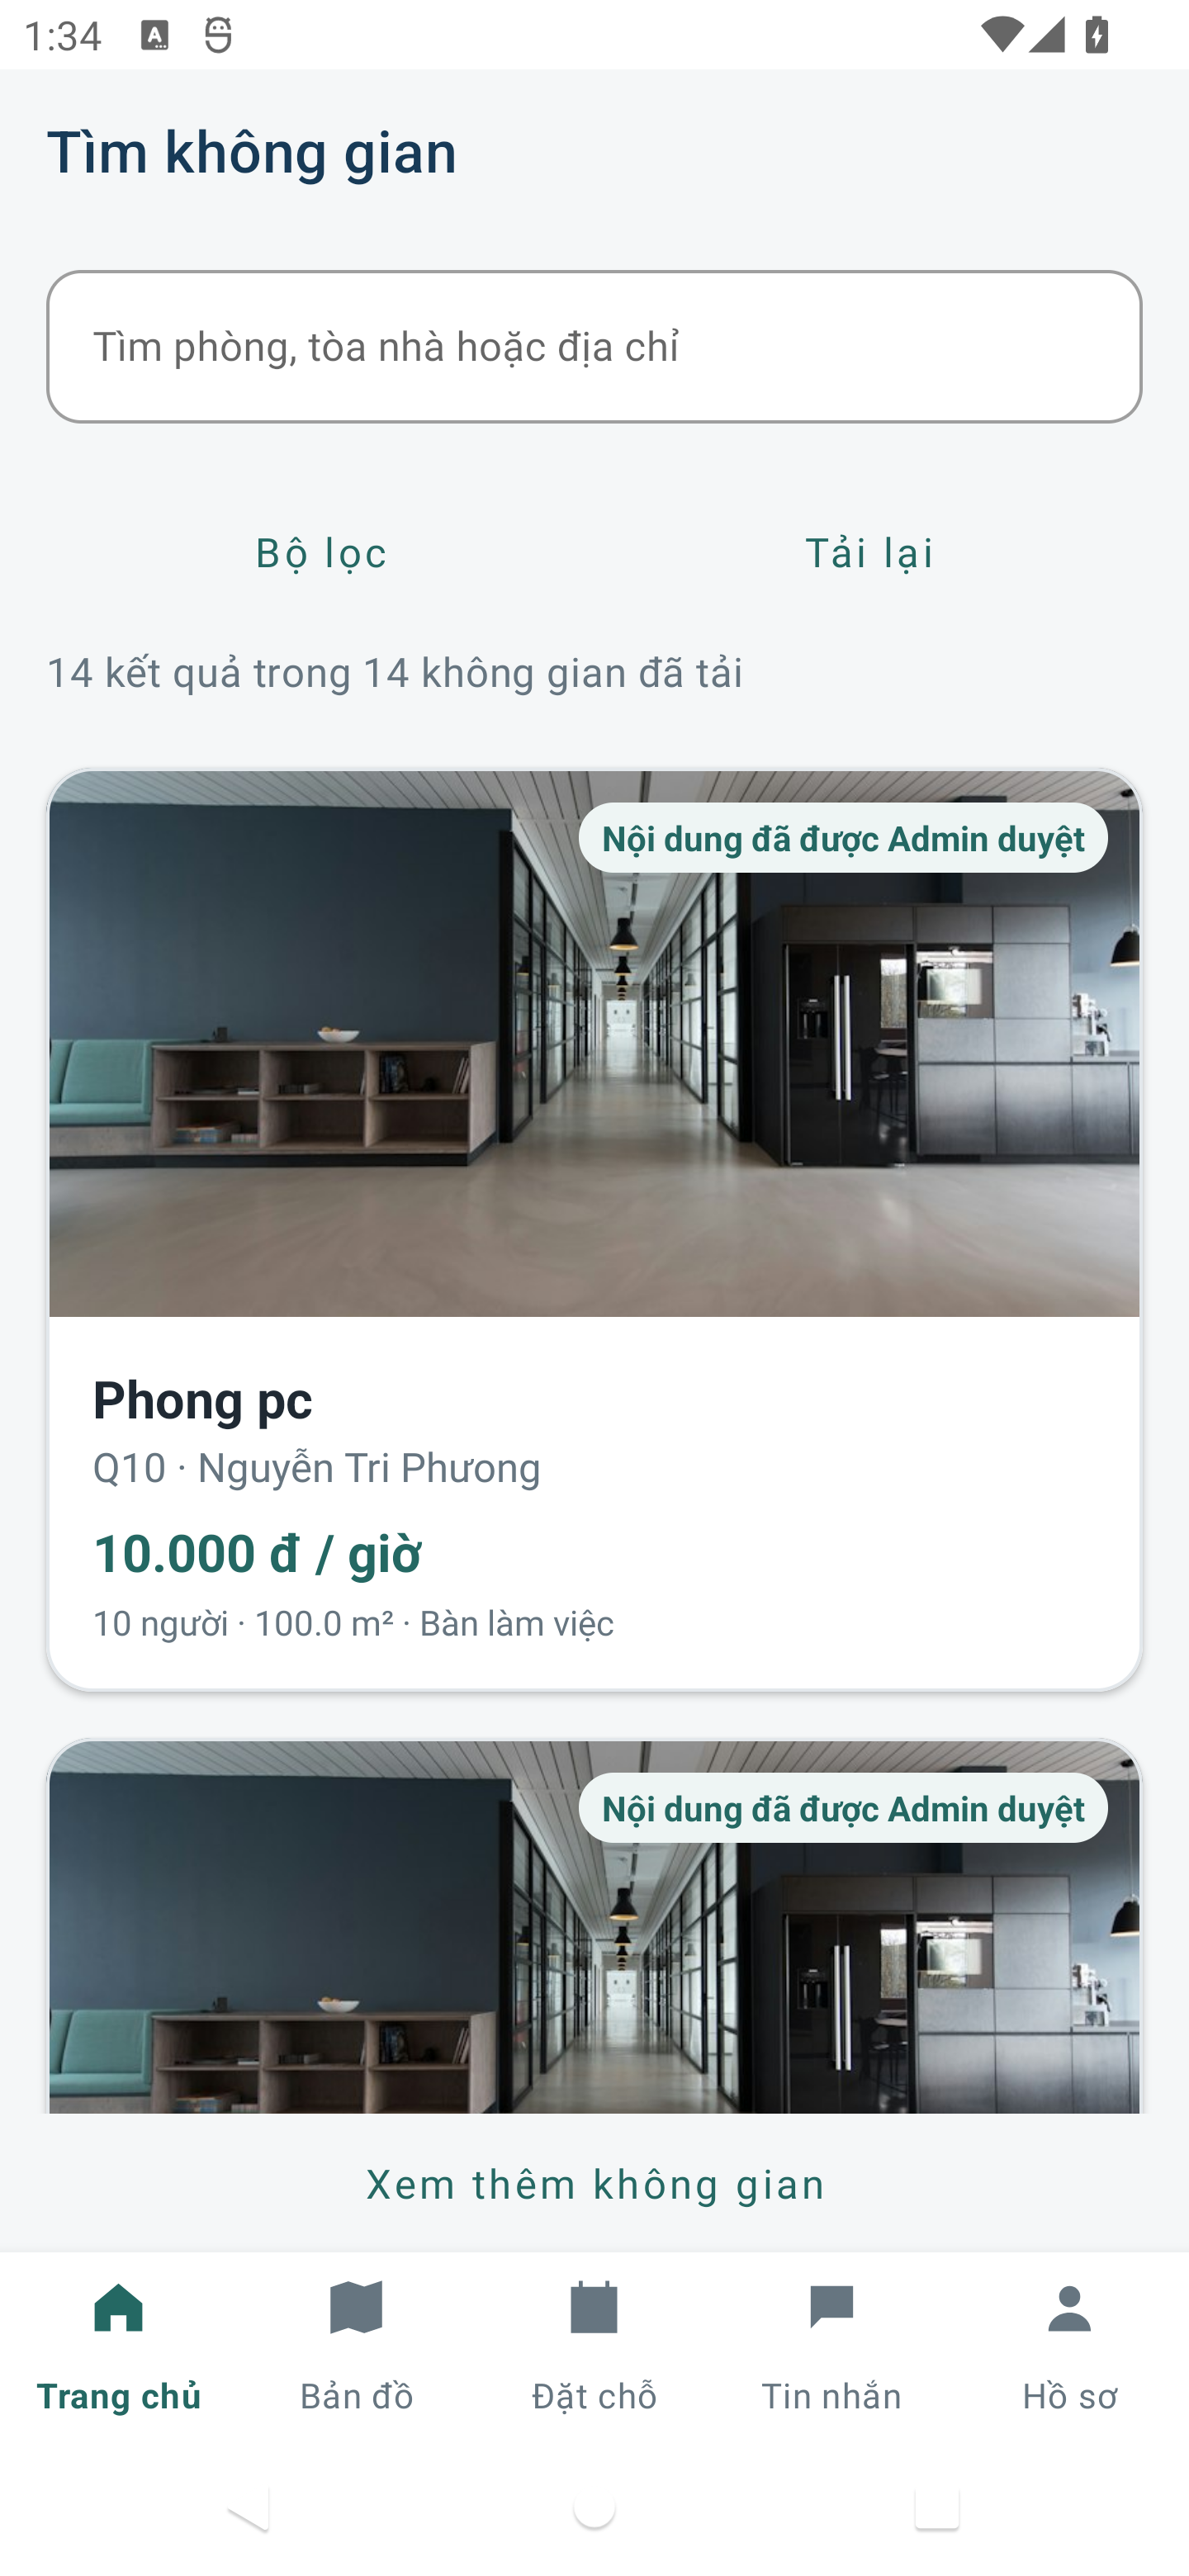
\includegraphics[width=\linewidth]{chapter5/final/home.png}\\[-1mm]
{\small (a) Danh sách phòng}
\end{minipage}\hspace{0.05\linewidth}%
\begin{minipage}[t]{0.34\linewidth}\centering
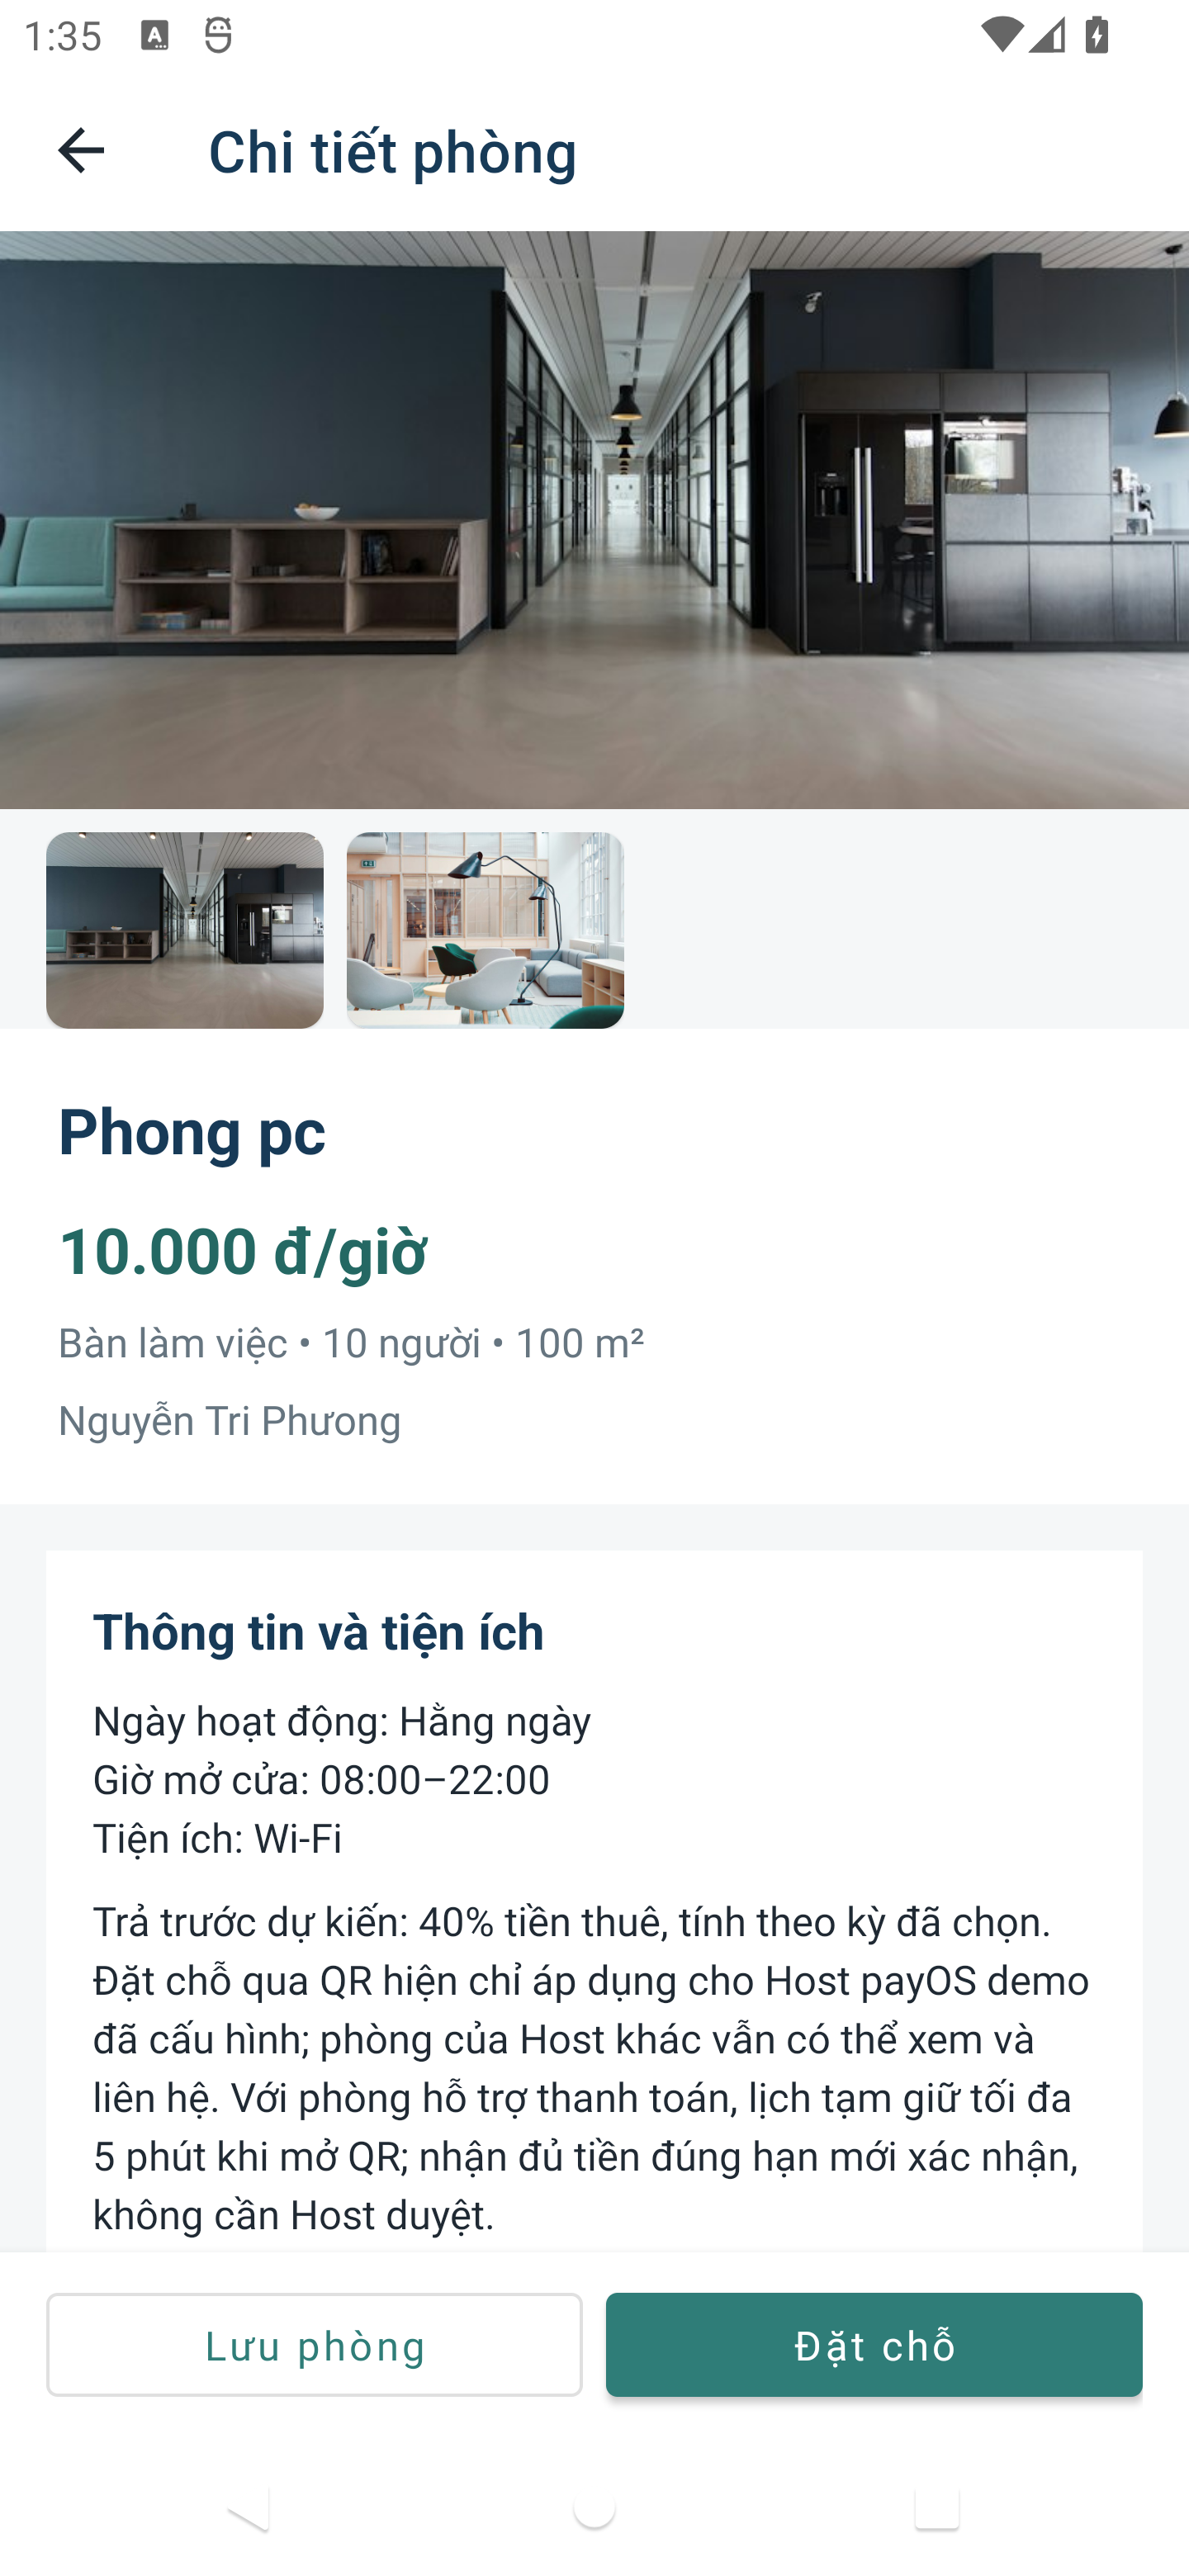
\includegraphics[width=\linewidth]{chapter5/final/detail.png}\\[-1mm]
{\small (b) Chi tiết phòng}
\end{minipage}
\caption{Từ danh sách không gian đến thông tin chi tiết}
\label{fig:actual-discovery}
\end{figure}

\subsubsection{Bản đồ và tìm đường}
\label{sec:screen-map}
Màn bản đồ kết hợp phòng từ Firestore với tọa độ tòa nhà, vị trí thiết bị hoặc tâm tìm kiếm do người dùng chọn. MapLibre Native dựng nền bản đồ từ MapTiler; MapRepository xử lý geocoding và tuyến ô tô từ openrouteservice. Khoảng cách dùng lọc lân cận được tính tại ứng dụng, chưa có truy vấn bán kính bằng geohash trên Firestore.

Hình~\ref{fig:actual-map} thể hiện điểm đến, tuyến đường và nút Xem phòng trên tablet. Nút này mở đúng chi tiết theo Room ID để tiếp tục đặt thuê. Địa điểm tham khảo được phân biệt với phòng trong app và dẫn tới nguồn tin; chúng chưa có chức năng đặt chỗ. Thời gian di chuyển là ước tính của tuyến, không bao gồm tình trạng giao thông trực tiếp.

\begin{figure}[H]\centering
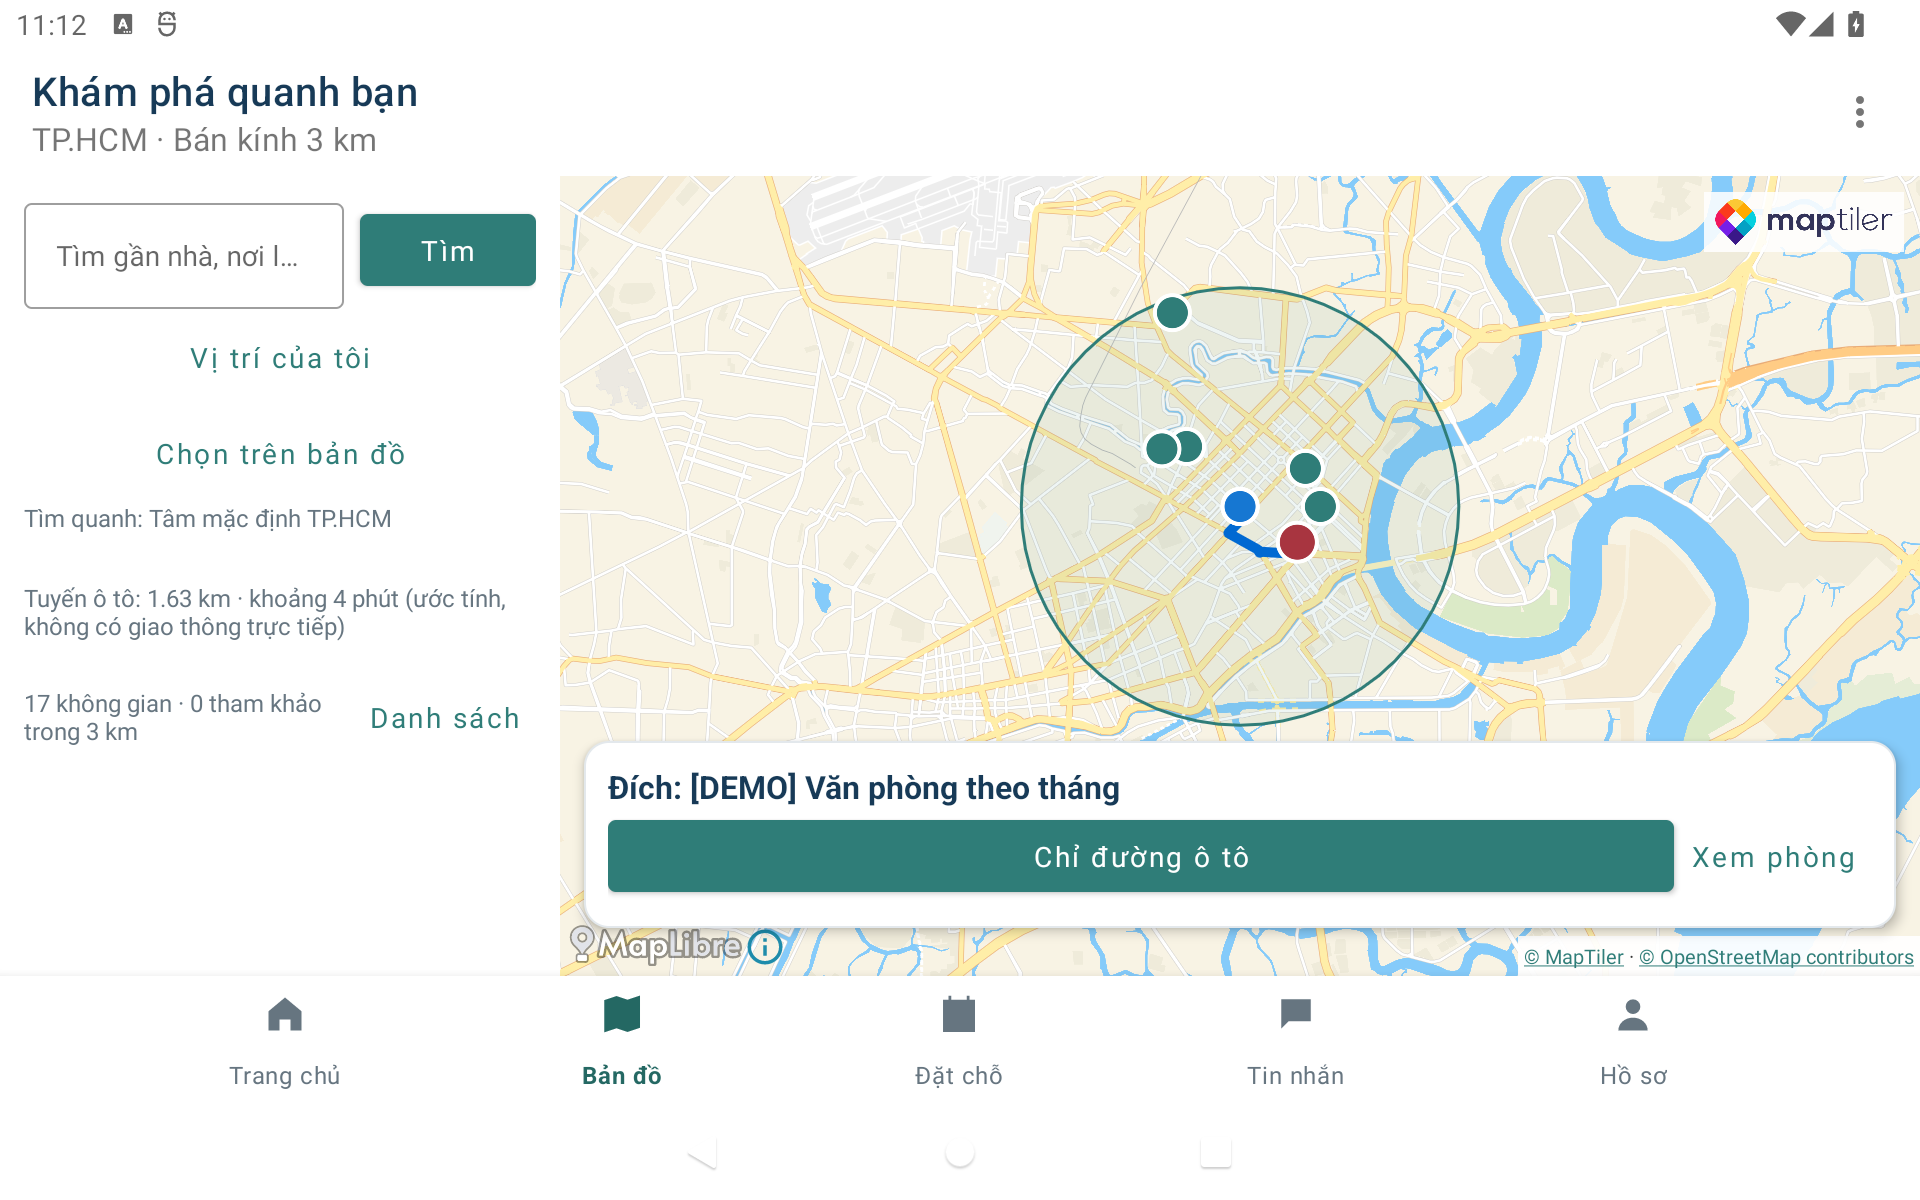
\includegraphics[width=0.96\linewidth]{chapter5/members/user-tablet-map-selected-landscape.png}
\caption{Chọn điểm đến, tìm đường và mở phòng từ bản đồ}
\label{fig:actual-map}
\end{figure}

\subsubsection{Đặt chỗ và thanh toán}
\label{sec:screen-payment}
BookingActivity hiển thị bộ chọn thời gian theo hình thức thuê của phòng. Sau khi kiểm tra lịch và giá, nút thanh toán tạo booking PENDING cùng khóa lịch tạm trong transaction và mở QR ngay. Thời hạn tối đa năm phút, không vượt giờ bắt đầu; mở lại phiên không gia hạn. Luồng mới không cần Host duyệt.

PaymentRepository gửi booking ID và ID token tới backend Java. Backend xác thực kênh Host demo, lấy khoản trả trước 40\% từ giá đã chốt và tạo giao dịch payOS. Đủ tiền đúng hạn mới cập nhật PAID/CONFIRMED; hết hạn chưa trả dẫn tới kết quả không thành công và nhả lịch sau đối soát. Listener cập nhật màn QR, thẻ tiếp tục thanh toán và thông báo điện thoại. Các màn và kết quả tương ứng được thể hiện tại Mục~\ref{sec:execution-booking-payment}. QR dùng cho thanh toán; Host ghi nhận việc nhận phòng bằng thao tác riêng.

\subsubsection{Quản lý lượt thuê, đánh giá và báo cáo}
\label{sec:screen-rentals}
MyBookingsActivity theo dõi booking theo UID người thuê, sắp thời điểm tạo giảm dần và lọc trạng thái trên giao diện. Trang chi tiết chỉ mở các thao tác còn hợp lệ; trước khi hủy, Repository kiểm tra lại người thực hiện, thời gian và trạng thái. Lịch sử được giữ sau khi khép lượt, đồng thời tách trạng thái tiền khỏi trạng thái sử dụng.

Hình~\ref{fig:actual-rentals} minh họa booking hết hạn chưa thanh toán trên tablet. Đánh giá chỉ được gửi cho lượt đã khép, có xác nhận sử dụng; ReviewRepository ghi một document \texttt{reviews/\{bookingId\}} cho mỗi booking, gồm điểm tổng quan và nhận xét. Báo cáo vi phạm ghi vào \texttt{reports}; người gửi theo dõi kết quả, Host phản hồi hồ sơ còn mở và Admin kết luận. Chức năng lưu lịch mở biểu mẫu của ứng dụng Lịch bằng Intent; người dùng xác nhận việc lưu và lịch thiết bị không tự đổi khi booking bị hủy.

\begin{figure}[H]\centering
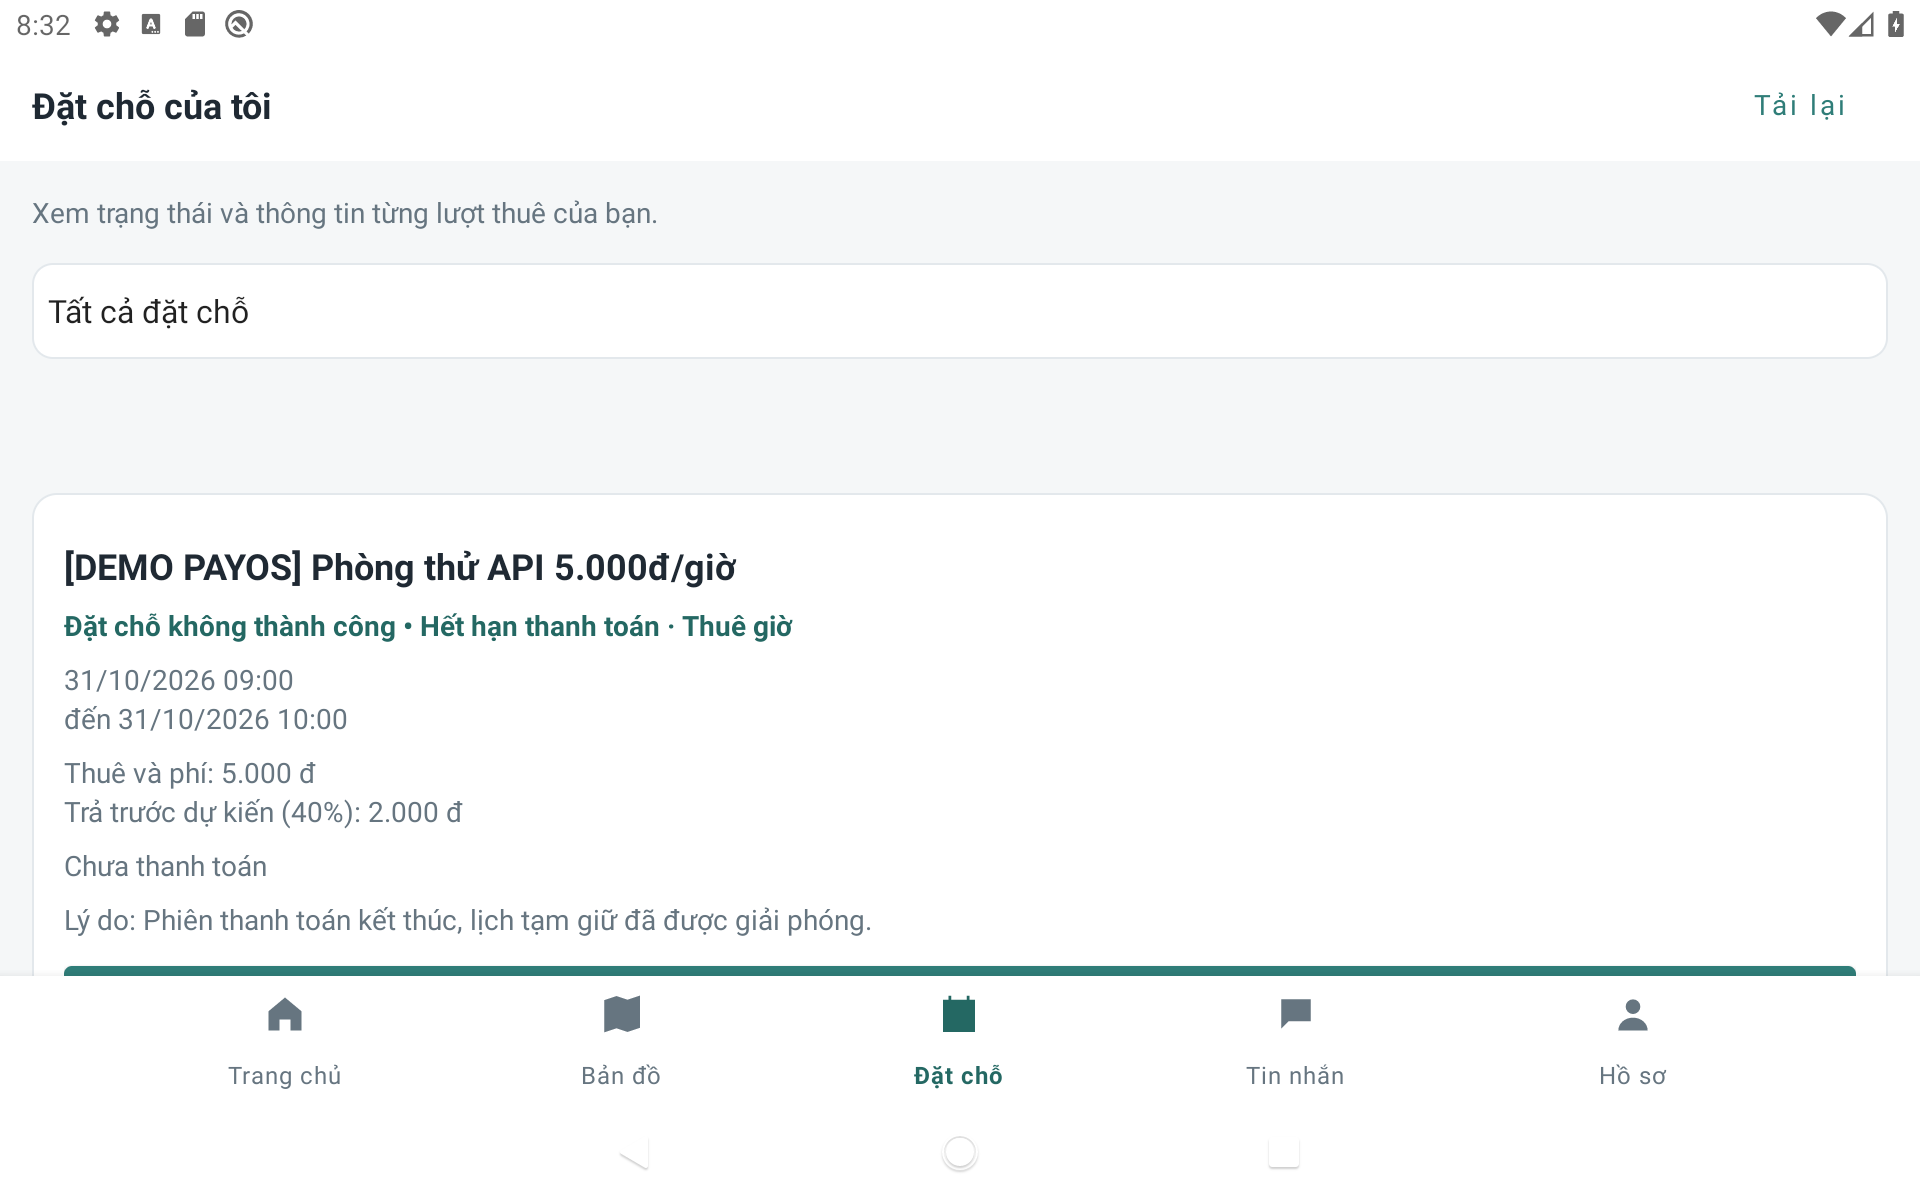
\includegraphics[width=0.96\linewidth]{chapter5/members/user-tablet-bookings-landscape.png}
\caption{Danh sách lượt thuê và kết quả hết hạn thanh toán}
\label{fig:actual-rentals}
\end{figure}

\subsubsection{Tin nhắn và thông báo}
\label{sec:screen-messages}
Inbox truy vấn \texttt{conversations} theo \texttt{memberUids}; mỗi hội thoại có subcollection \texttt{messages}, sắp bằng \texttt{sequence} và giới hạn số tin tải. Transaction gửi tin ghi message, preview, thứ tự và bộ đếm nhận; mốc đọc chỉ tăng cho bên đang đọc. Conversation ID theo cặp người thuê và Host cho phép tiếp tục trao đổi mà không tạo một hội thoại mới cho mỗi lần mở phòng.

Hình~\ref{fig:actual-messages} thể hiện danh sách hội thoại và màn trao đổi với Host của phòng PAYOS. Hội thoại mới hiển thị phòng ngữ cảnh và ô gửi tin trước khi có nội dung trao đổi. Hộp cập nhật tổng hợp sự kiện booking, hội thoại và báo cáo, còn \texttt{noticeReads} chỉ lưu mốc đã đọc. PaymentReminderService hiển thị phiên còn hạn và đổi thông báo theo kết quả, như Hình~\ref{fig:booking-resume-notification}; quyền thông báo không quyết định trạng thái thanh toán trên server.

\begin{figure}[H]\centering
\begin{minipage}[t]{0.34\linewidth}\centering
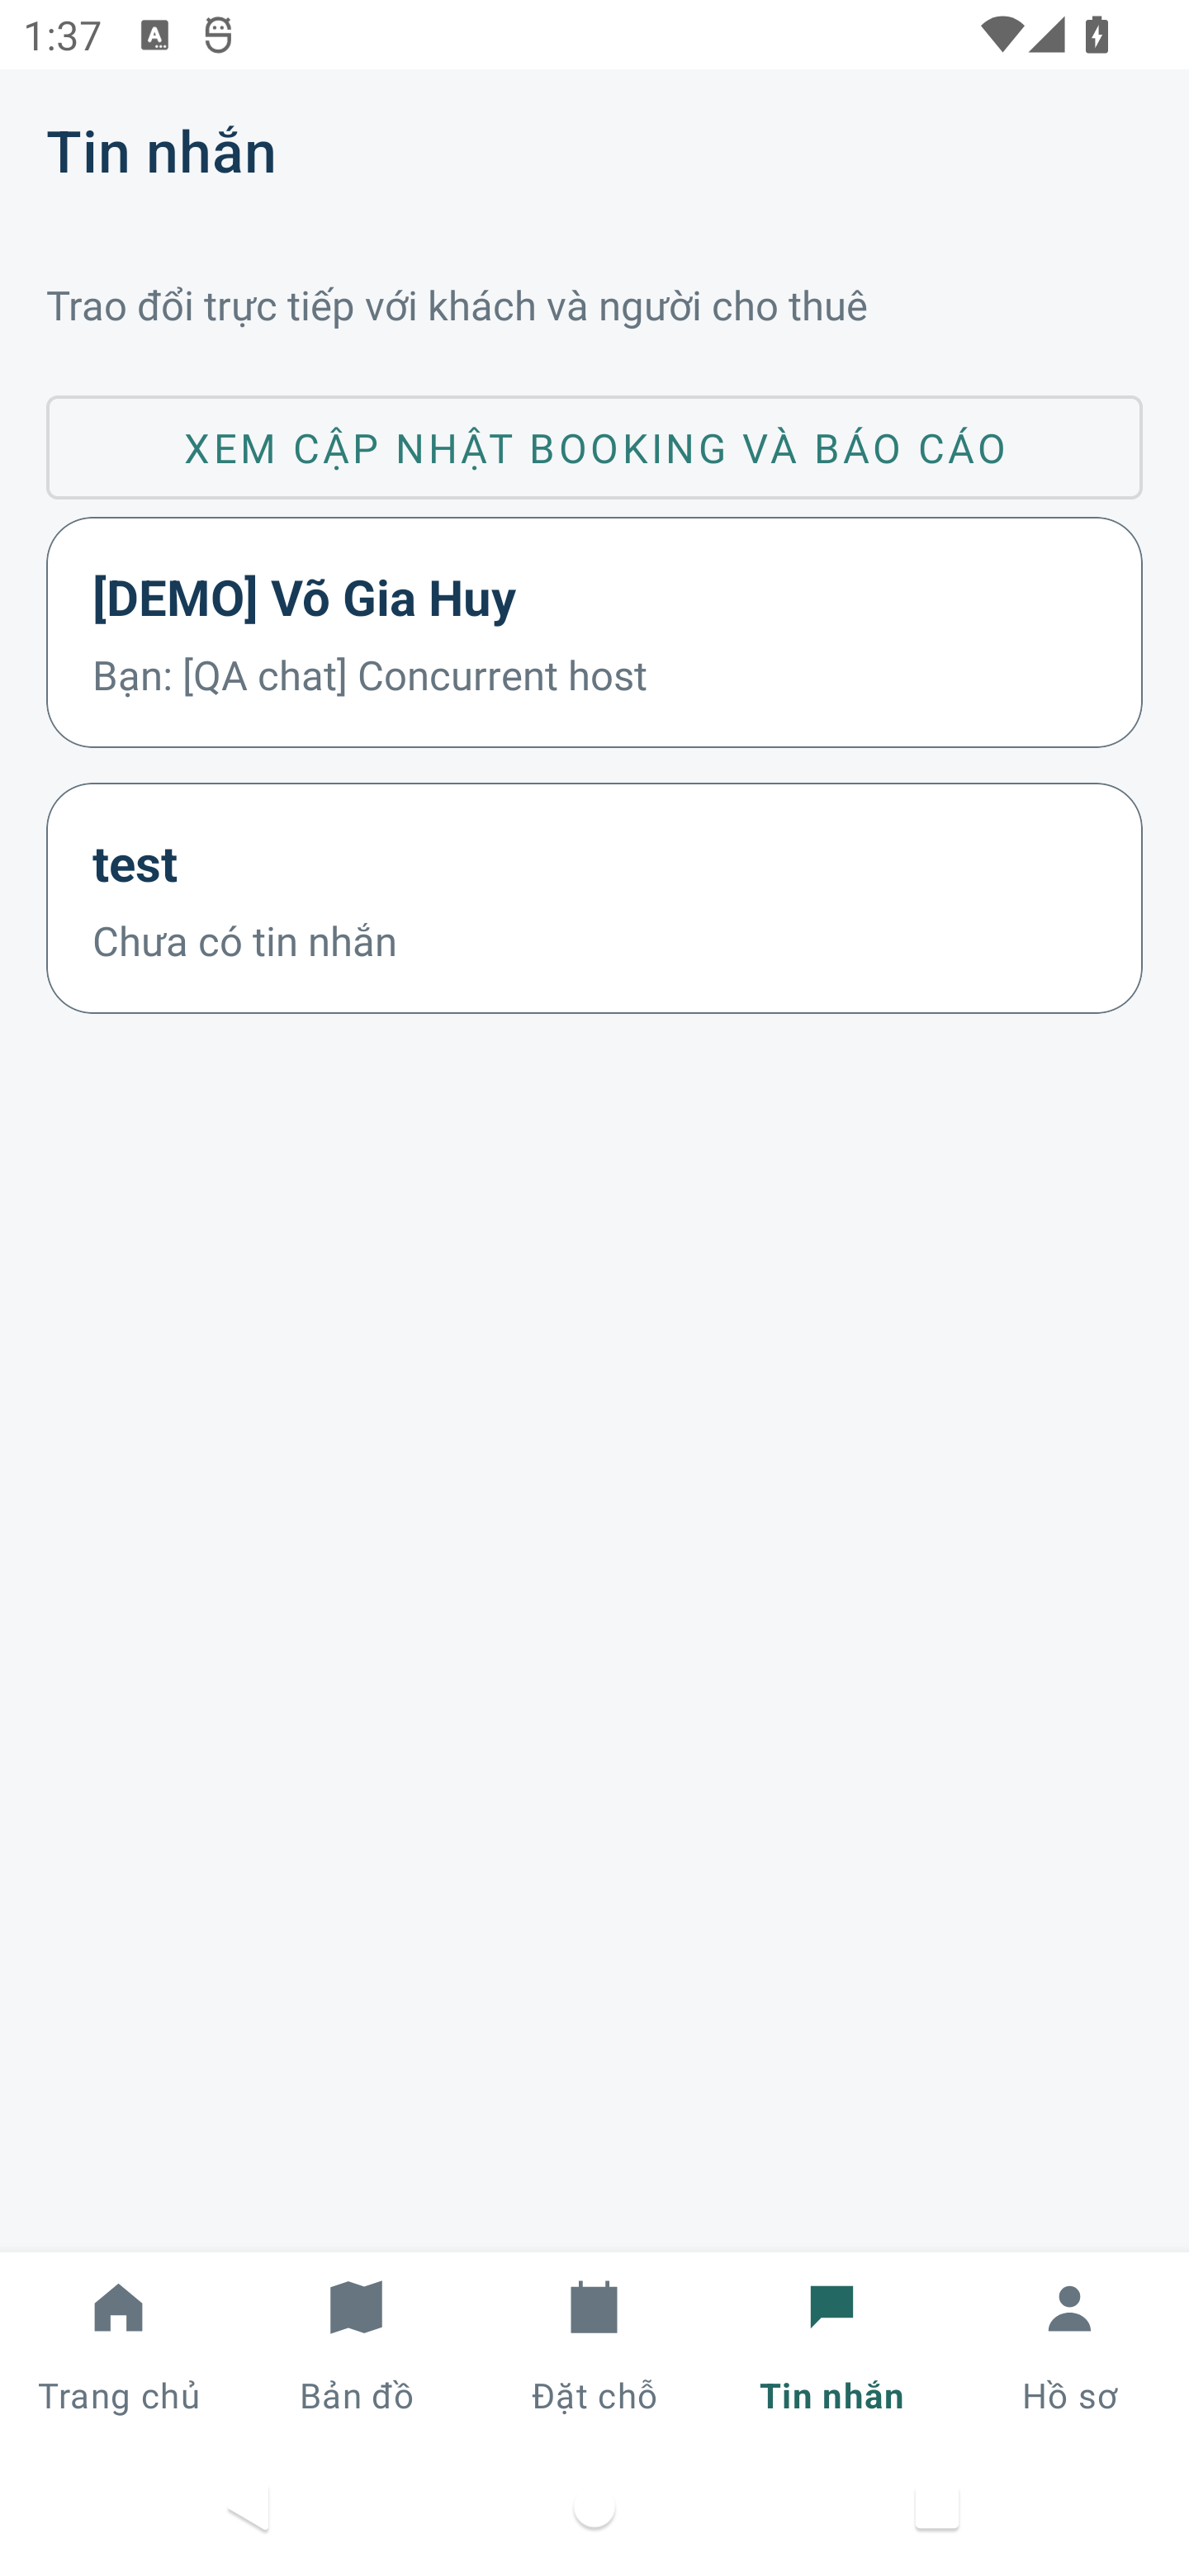
\includegraphics[width=\linewidth]{chapter5/final/conversations.png}\\[-1mm]
{\small (a) Danh sách hội thoại DEMO}
\end{minipage}\hspace{0.05\linewidth}%
\begin{minipage}[t]{0.34\linewidth}\centering
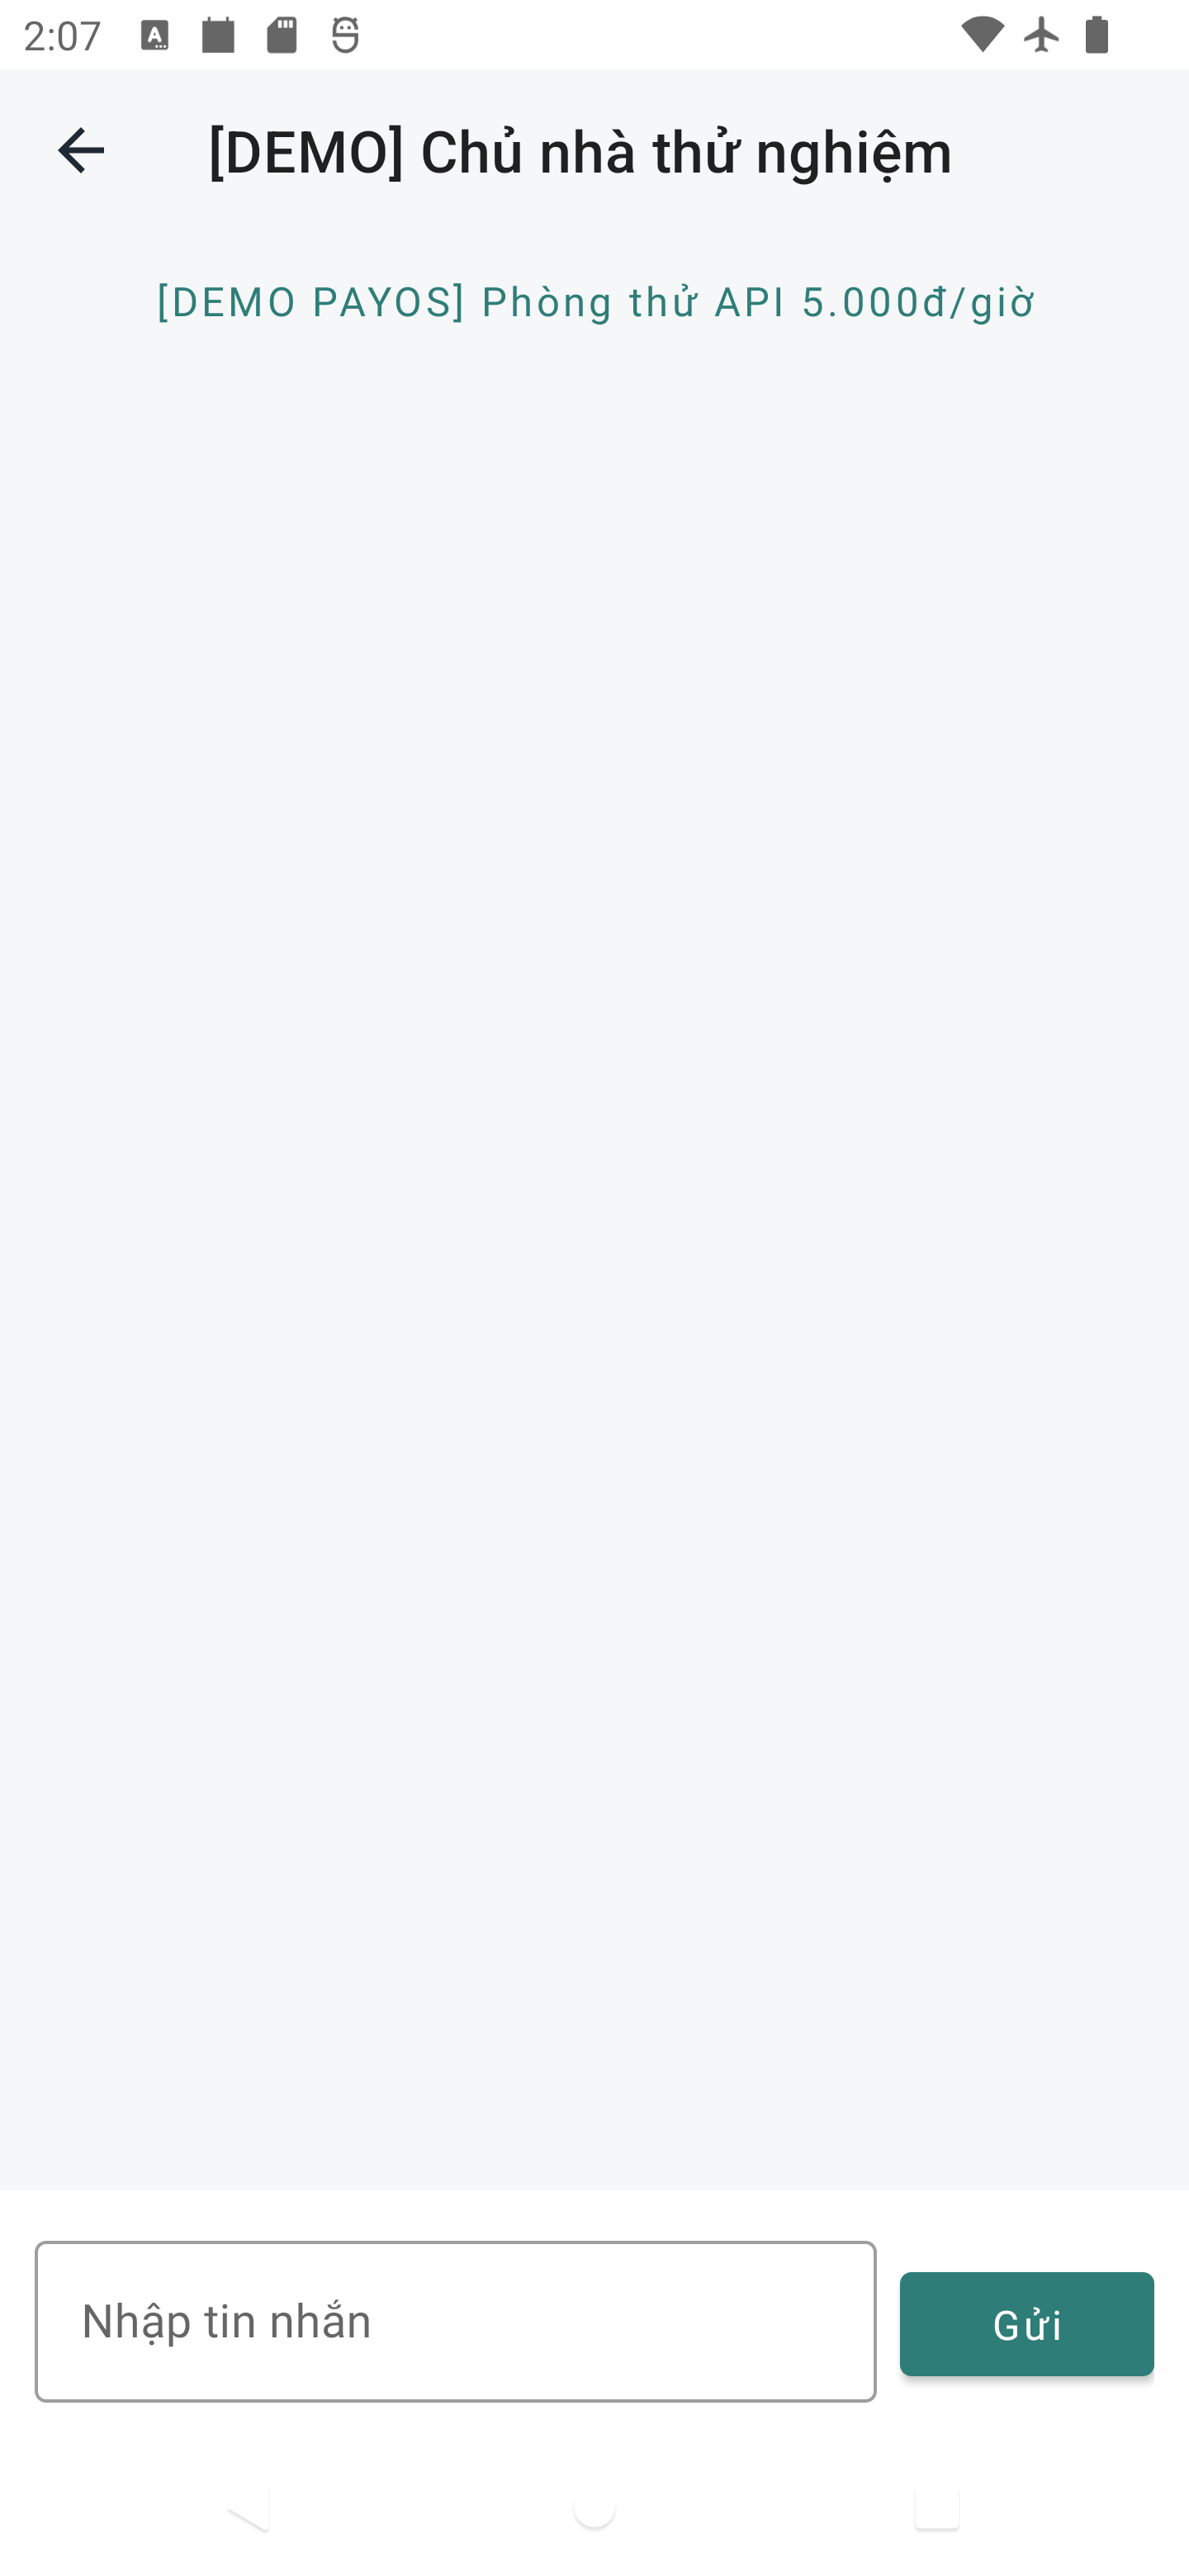
\includegraphics[width=\linewidth]{chapter5/final/conversation-detail.png}\\[-1mm]
{\small (b) Hội thoại gắn với phòng}
\end{minipage}
\caption{Danh sách hội thoại và màn trao đổi với Host}
\label{fig:actual-messages}
\end{figure}

\FloatBarrier
\subsubsection{Các màn hình dành cho Host}
\label{sec:screen-host}
Kênh Host tổ chức tổng quan, không gian, booking, tin nhắn và tài khoản. Đơn xin quyền Host nằm tại \texttt{hostApplications/\{uid\}}, gồm thông tin liên hệ và hai ảnh giấy tờ DEMO; hồ sơ chỉ được cấp quyền khi Admin chấp thuận. Sau đó Host tạo tòa nhà, phòng và cấu hình cho thuê. Hình~\ref{fig:actual-host-editor} minh họa danh sách tòa nhà và biểu mẫu đăng phòng; dữ liệu được gửi qua HostViewModel tới HostRepository.

\begin{figure}[!htbp]\centering
\begin{minipage}[t]{0.40\linewidth}\centering\vspace{0pt}
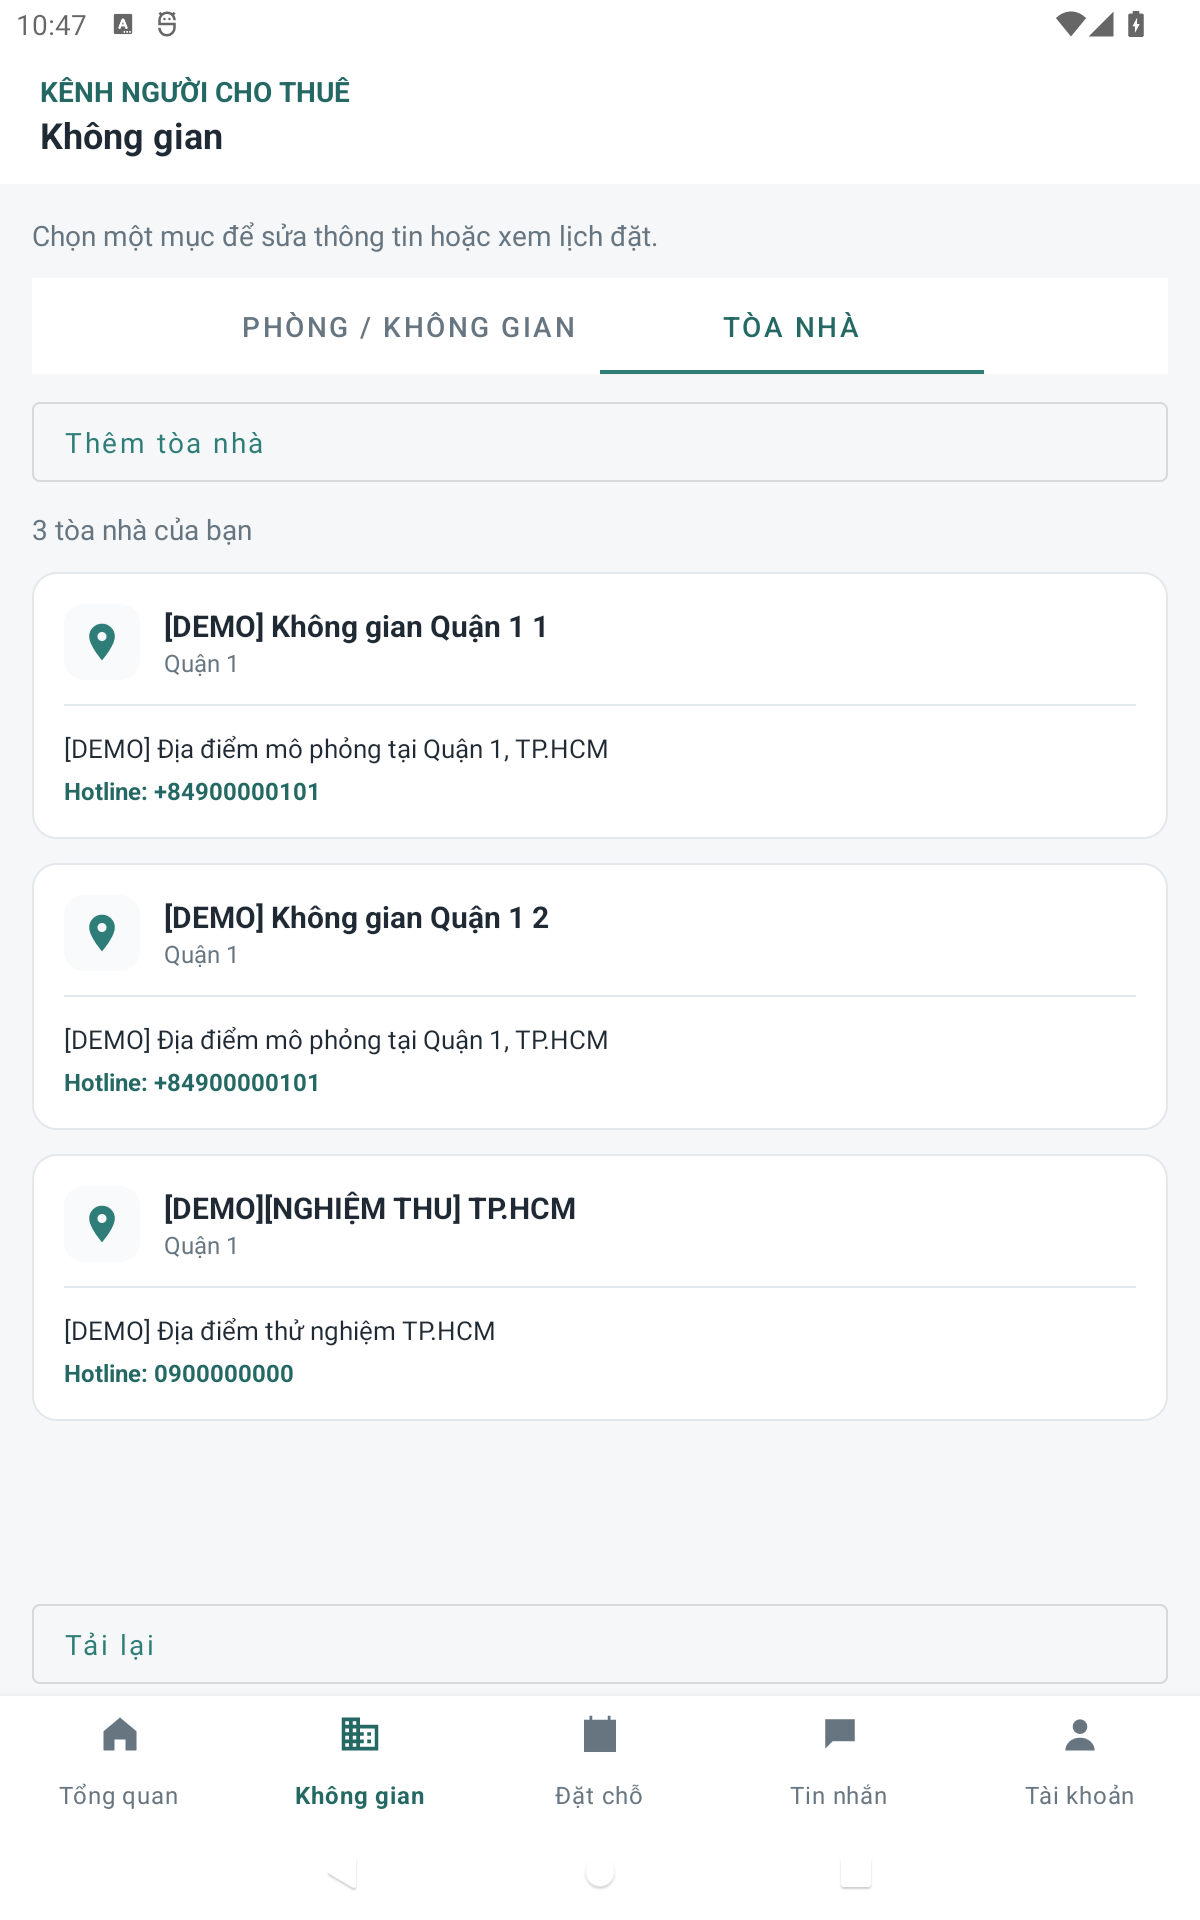
\includegraphics[height=0.40\textheight,width=\linewidth,keepaspectratio]{chapter5/members/host-tablet-buildings-portrait.png}\\[-1mm]
{\small (a) Tòa nhà của Host trên tablet}
\end{minipage}\hspace{0.05\linewidth}%
\begin{minipage}[t]{0.30\linewidth}\centering\vspace{0pt}
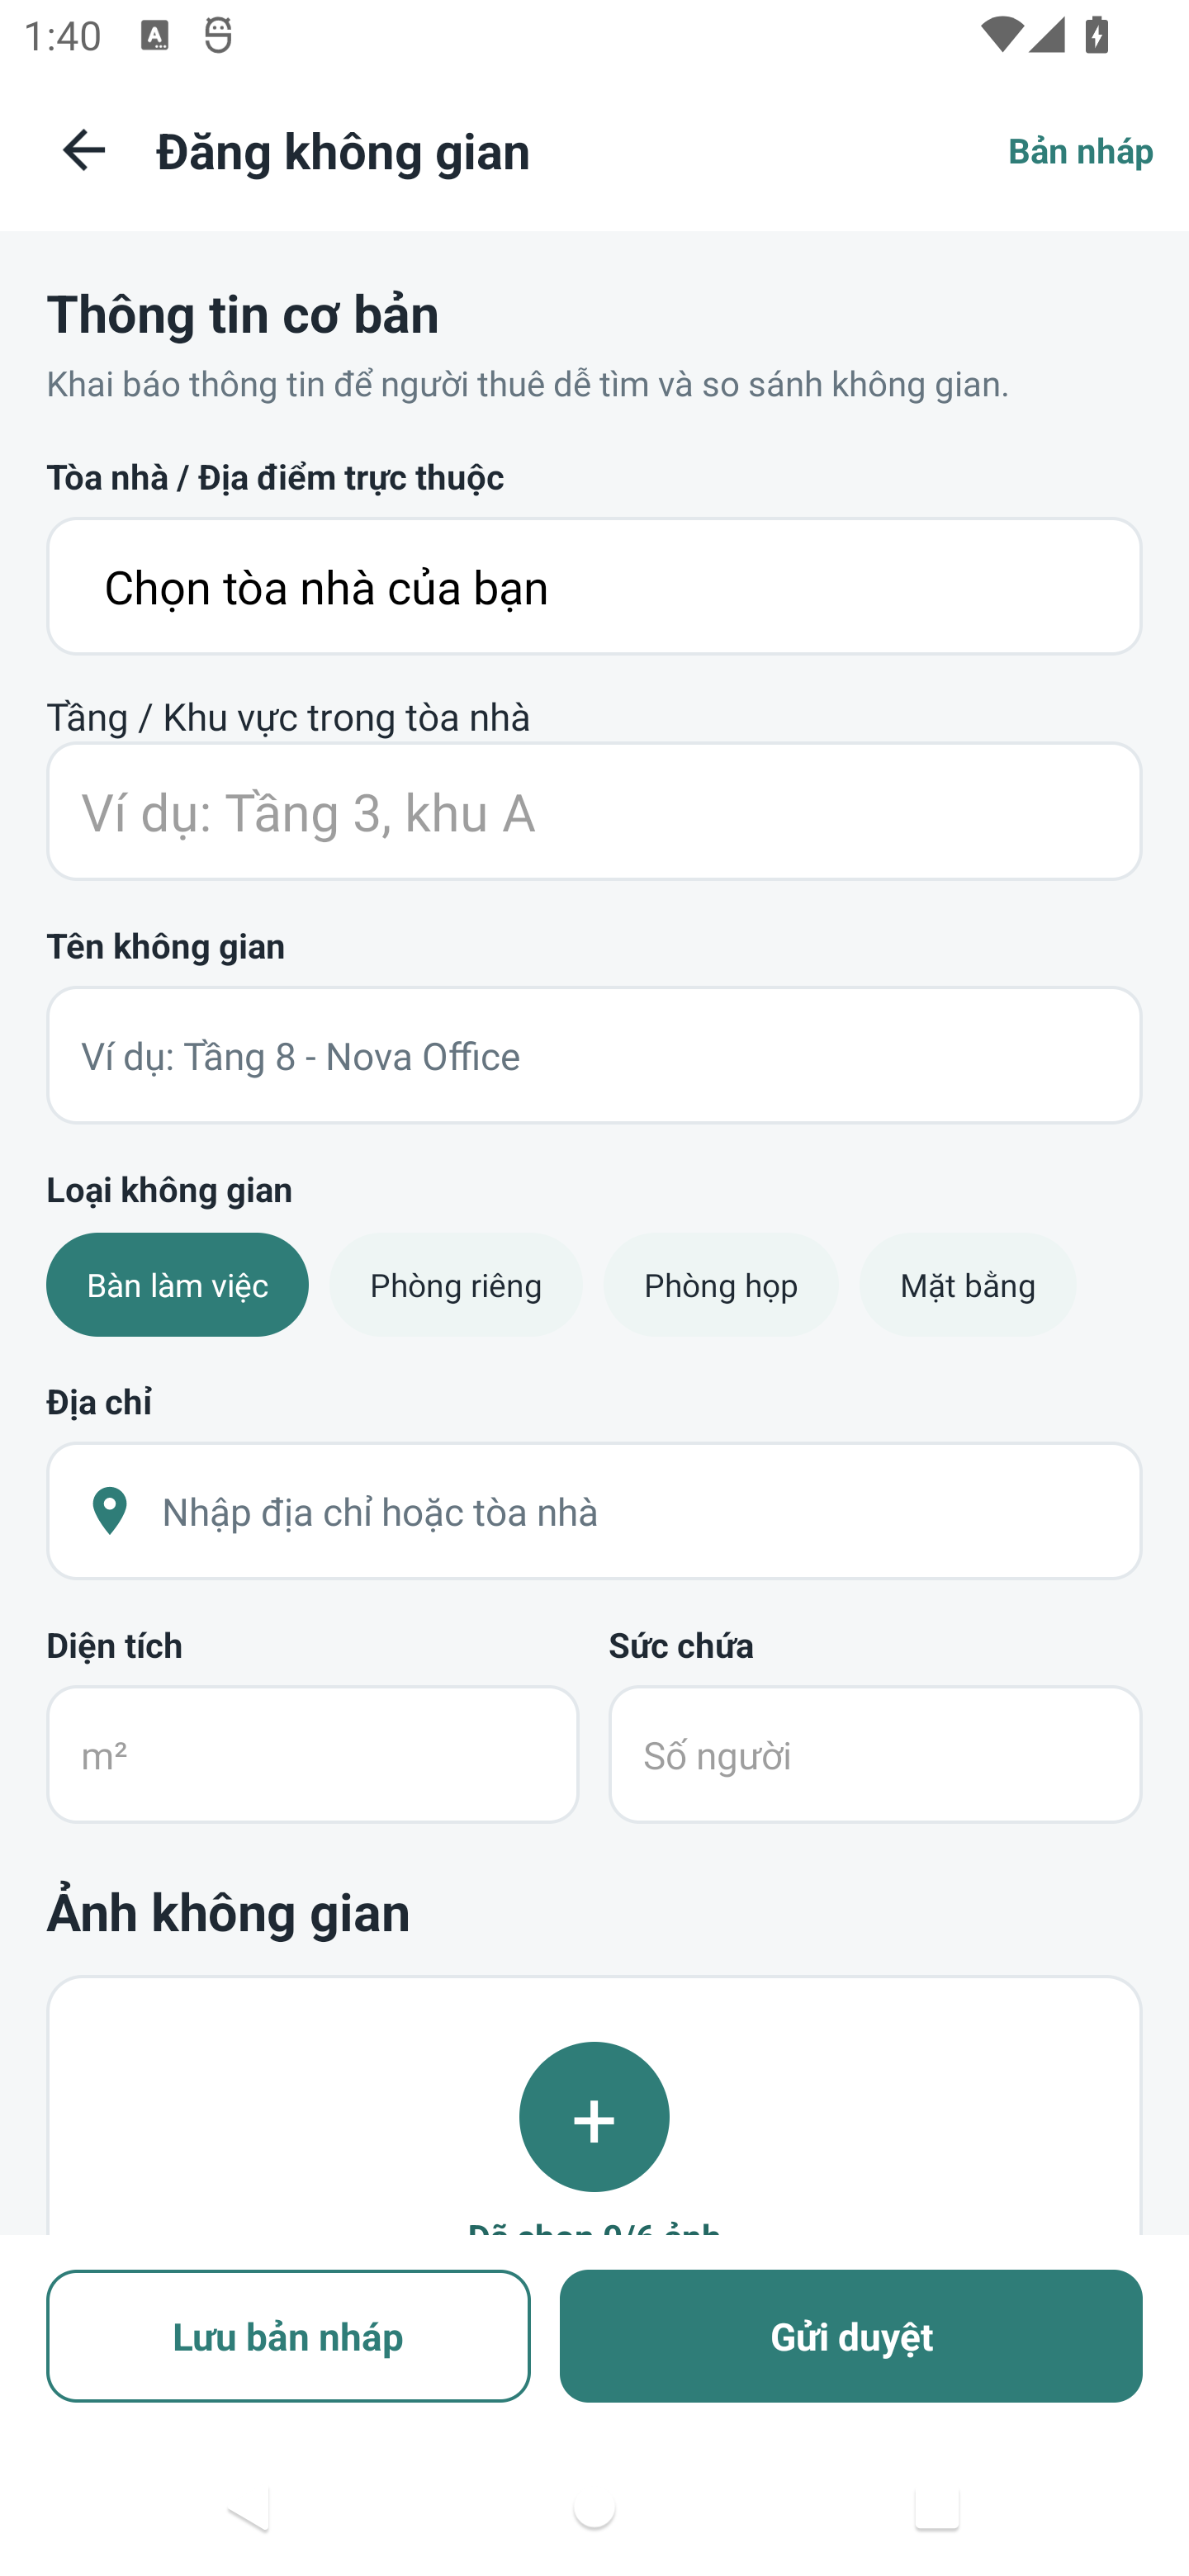
\includegraphics[height=0.40\textheight,width=\linewidth,keepaspectratio]{chapter5/final/host-create.png}\\[-1mm]
{\small (b) Biểu mẫu phòng trên điện thoại}
\end{minipage}
\caption{Quản lý địa điểm và khai báo không gian cho thuê}
\label{fig:actual-host-editor}
\end{figure}

Màn tổng quan ở Hình~\ref{fig:actual-host-overview} tổng hợp số không gian, tin chờ xét duyệt, phòng đang hiển thị và yêu cầu thuê của tài khoản hiện tại. Host chuyển từ các chỉ số này tới danh sách tương ứng. Số liệu được tính trên phòng và booking thuộc Host; phiên đang chờ thanh toán được phân biệt với lượt đã xác nhận.

\begin{figure}[!htbp]\centering
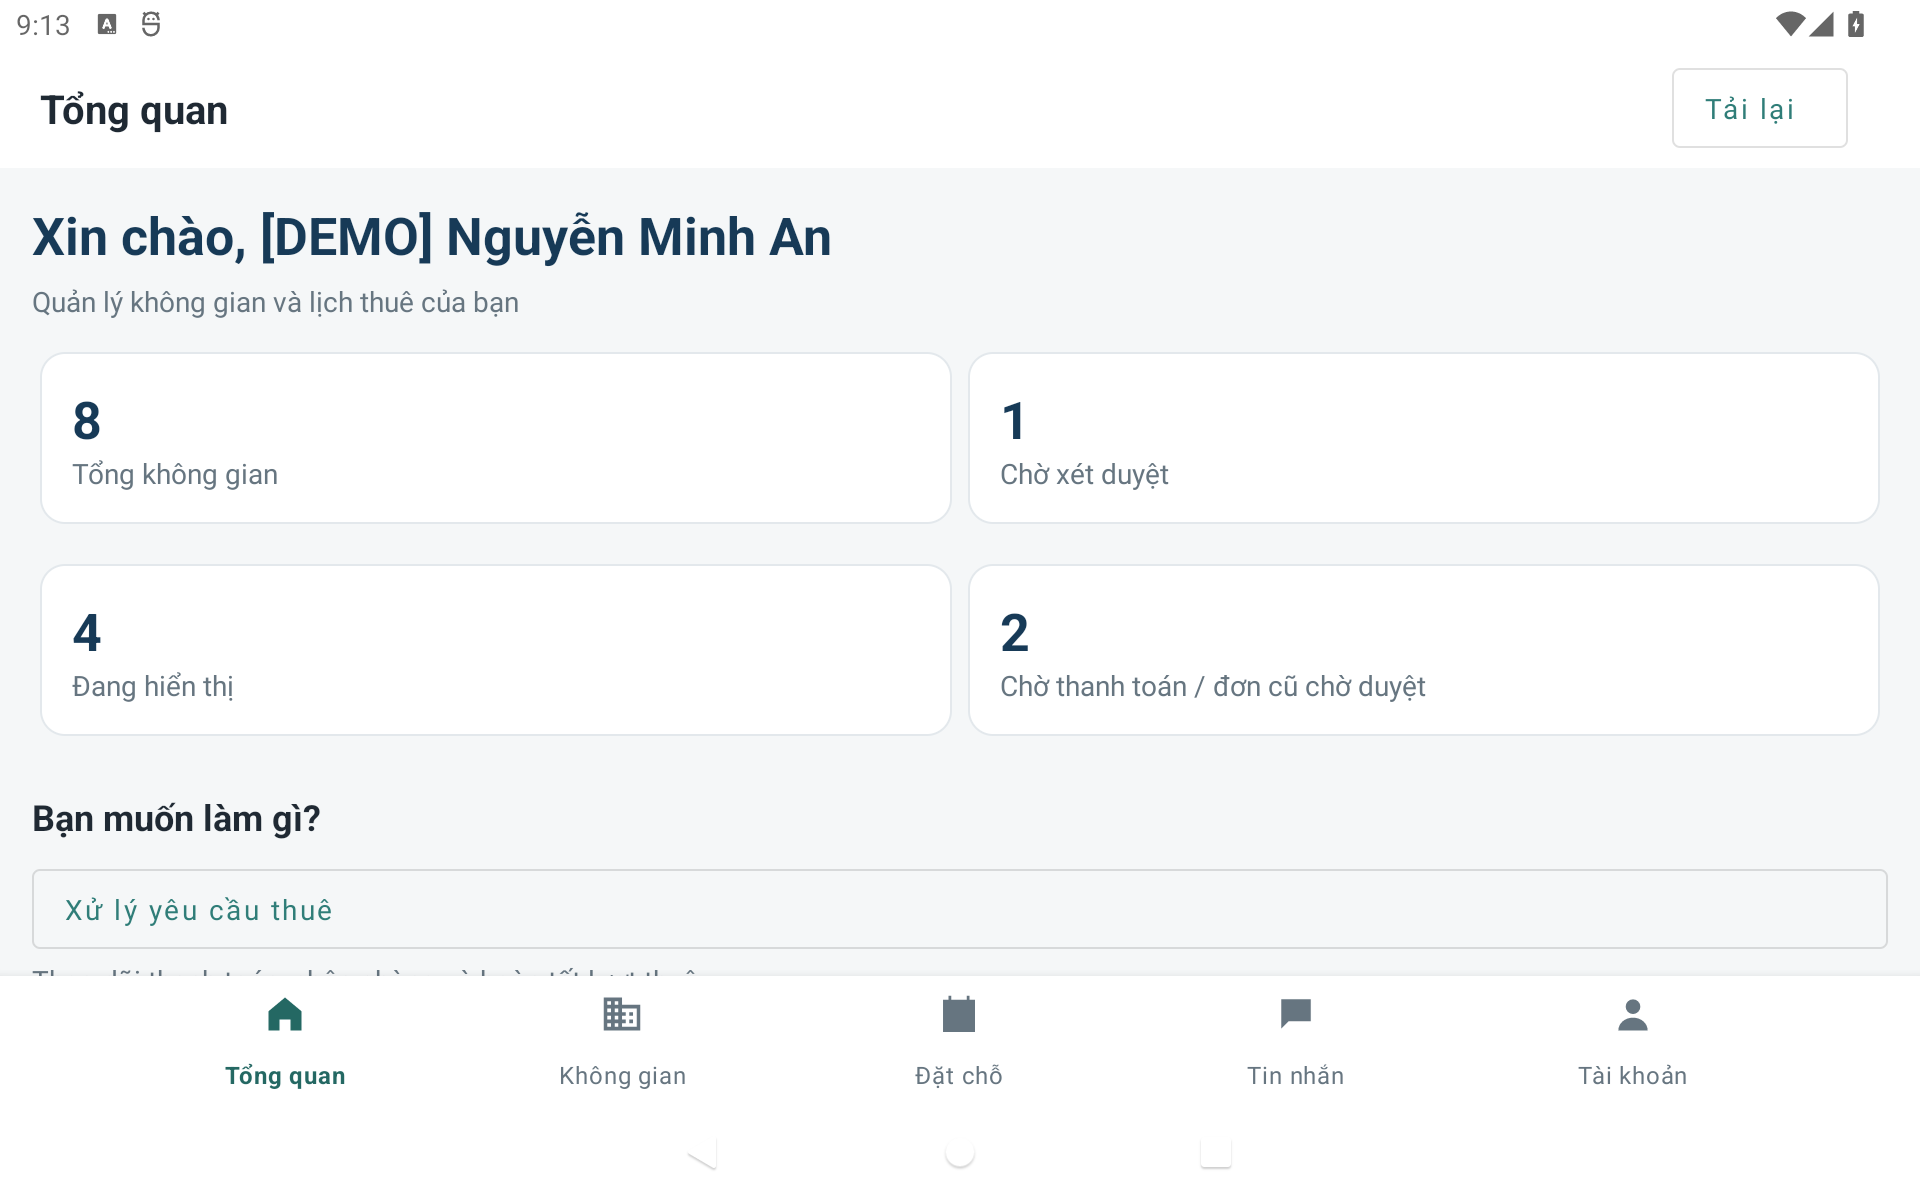
\includegraphics[width=0.96\linewidth]{chapter5/members/host-tablet-overview-landscape.png}
\caption{Tổng quan quản lý không gian của Host trên tablet}
\label{fig:actual-host-overview}
\end{figure}

Phòng lưu vào \texttt{rooms}, gắn Building và owner UID. Host chọn thuê giờ hoặc tháng/quý, khai báo giá, lịch hoạt động, ngày khóa và khoảng khóa; cấu hình ảnh giới hạn sáu tệp. HostViewModel tải ảnh qua Cloudinary trước khi ghi URL. Bản nháp và tin chờ duyệt có trạng thái riêng; quyền Host không thay thế quyết định duyệt từng bài đăng. Việc đổi chế độ hoặc lịch chịu kiểm tra các booking còn giữ chỗ để không làm sai kỳ thuê đã có.

\begin{figure}[!htbp]\centering
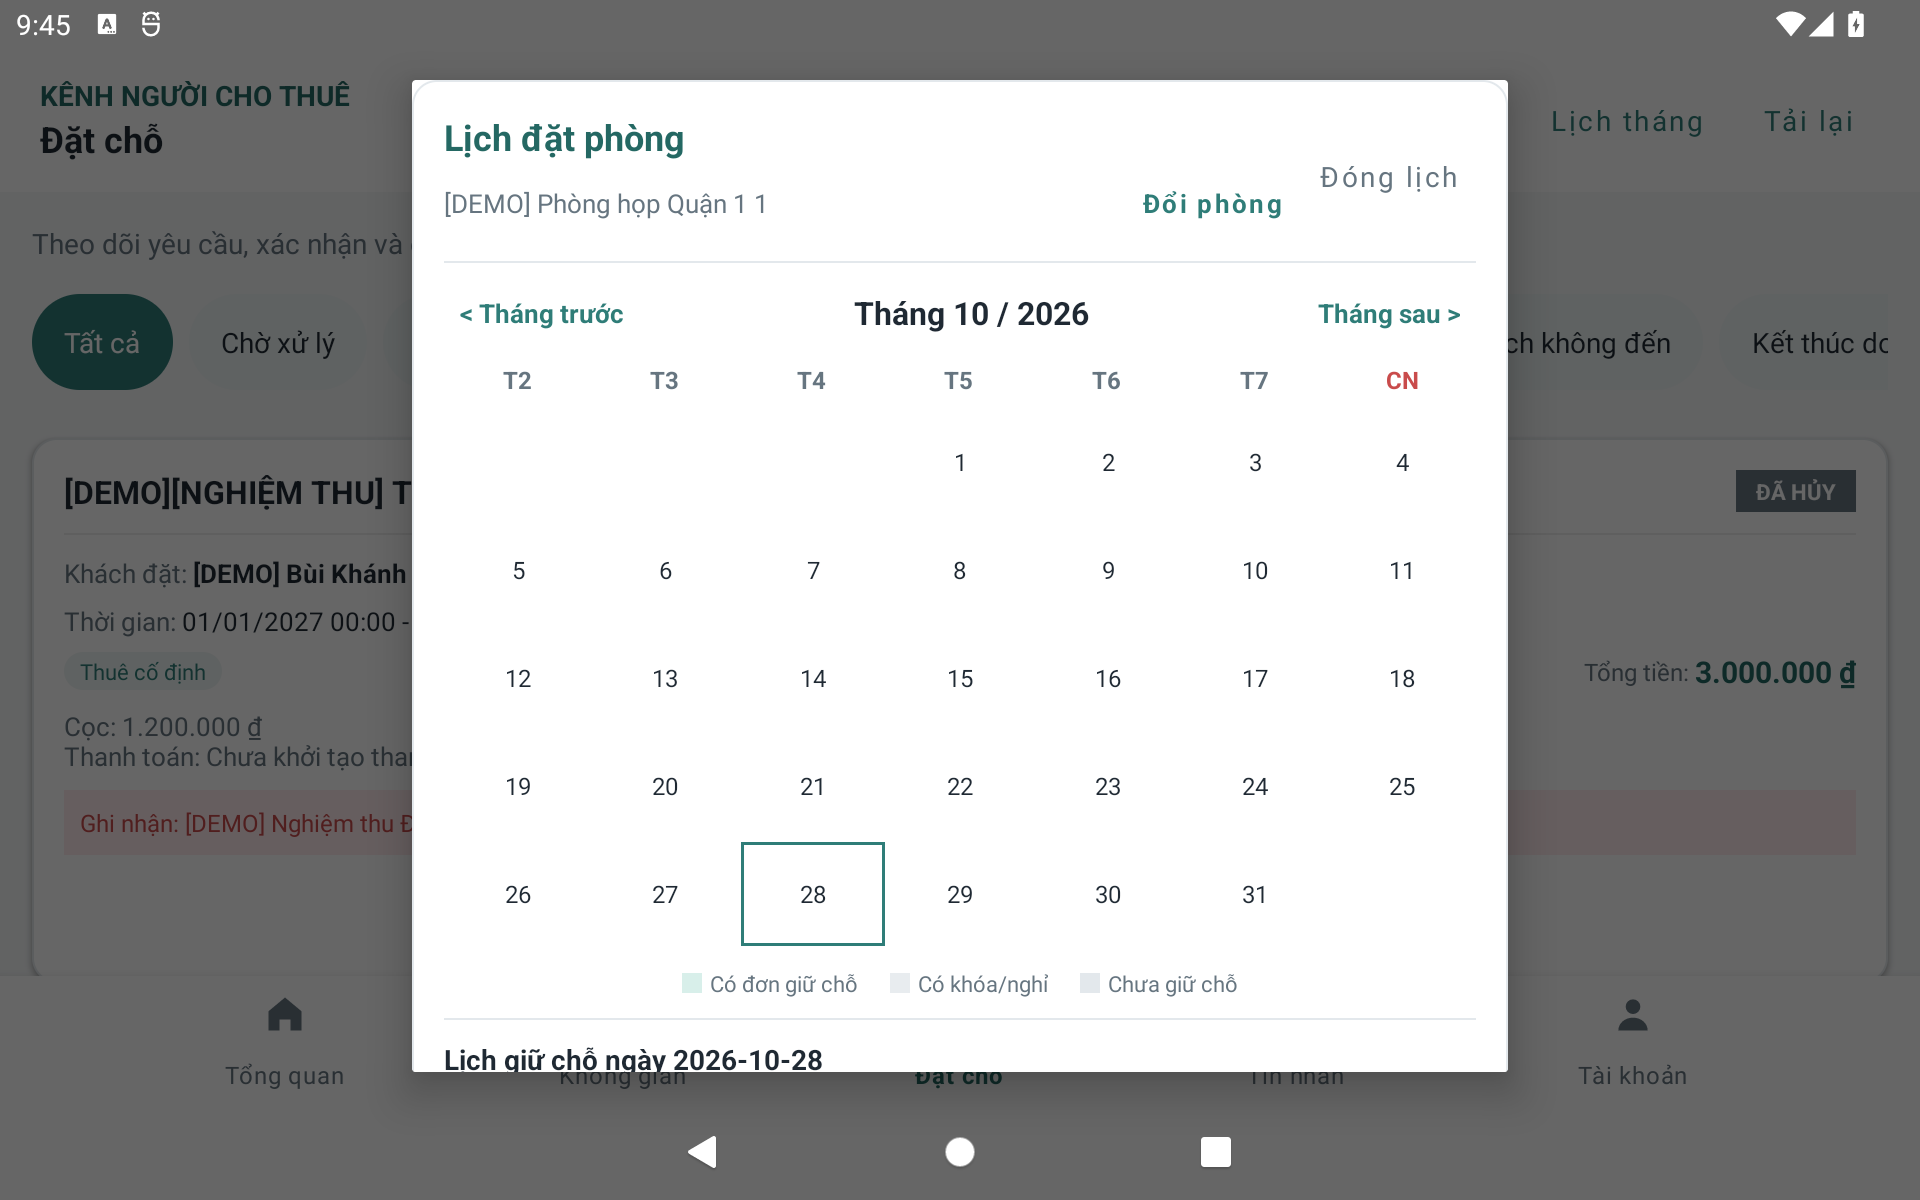
\includegraphics[width=0.96\linewidth]{chapter5/members/host-tablet-calendar-landscape.png}
\caption{Lịch đặt phòng theo tháng trong kênh Host}
\label{fig:actual-host-calendar}
\end{figure}
\FloatBarrier

Danh sách không gian phân biệt trạng thái xét duyệt với trạng thái hiển thị. Lịch tại Hình~\ref{fig:actual-host-calendar} tổng hợp khoảng giữ chỗ, ngày khóa và cho xem chi tiết theo ngày. Host theo dõi booking đã thanh toán, ghi nhận khách đến trong kỳ thuê, hoàn tất hoặc ghi nhận không đến theo điều kiện nghiệp vụ. Hồ sơ minh chứng LOCATION/PHOTOS và phản hồi báo cáo được xử lý tại các màn riêng.

\FloatBarrier
\subsubsection{Các màn hình dành cho Admin}
\label{sec:admin-implementation}

Kênh Admin tập trung các công việc xét duyệt, quản lý quyền, xử lý báo cáo và tra cứu nhật ký. Màn hình tổng quan cung cấp lối vào từng nhóm; các hàng đợi được trình bày bằng thẻ hồ sơ hoặc tin đăng. AdminViewModel giữ nhóm đang chọn và trạng thái request, còn AdminRepository truy vấn theo loại đối tượng. Bộ đếm hàng đợi được tính từ dữ liệu vừa tải trong giới hạn truy vấn, không phải số liệu tổng hợp toàn hệ thống.

Hàng đợi Host lấy những đơn đang PENDING từ \texttt{hostApplications}. Mỗi thẻ gồm thông tin người nộp, nội dung hồ sơ và tệp giấy tờ DEMO. Giao diện yêu cầu mở các tệp minh chứng trước khi gửi quyết định chấp thuận. Trong transaction xét duyệt, Repository đọc lại quyền Admin, trạng thái đơn và hồ sơ người nộp. Khi chấp thuận, trạng thái đơn, quyền HOST trong \texttt{users}, bản chiếu \texttt{publicHosts} và audit được cập nhật cùng thao tác. Khi từ chối, lý do được lưu để người nộp có thể bổ sung hồ sơ.

\IfFileExists{Resources/chapter5/admin-overview.png}{%
Màn hình tổng quan trong Hình~\ref{fig:admin-overview-review}(a) tổ chức các lối vào xét duyệt, quản lý, báo cáo và nhật ký. Khi chọn xét duyệt không gian, Admin nhận danh sách phòng PENDING\_REVIEW như Hình~\ref{fig:admin-overview-review}(b). Mỗi thẻ có ảnh, thông tin tóm tắt và nút mở nội dung đầy đủ trước khi duyệt hoặc từ chối. Repository kiểm lại chủ sở hữu và tòa nhà trước khi ghi quyết định; xét duyệt tin đăng độc lập với cấp quyền Host.
\begin{figure}[H]
\centering
\begin{minipage}[t]{0.40\linewidth}\centering
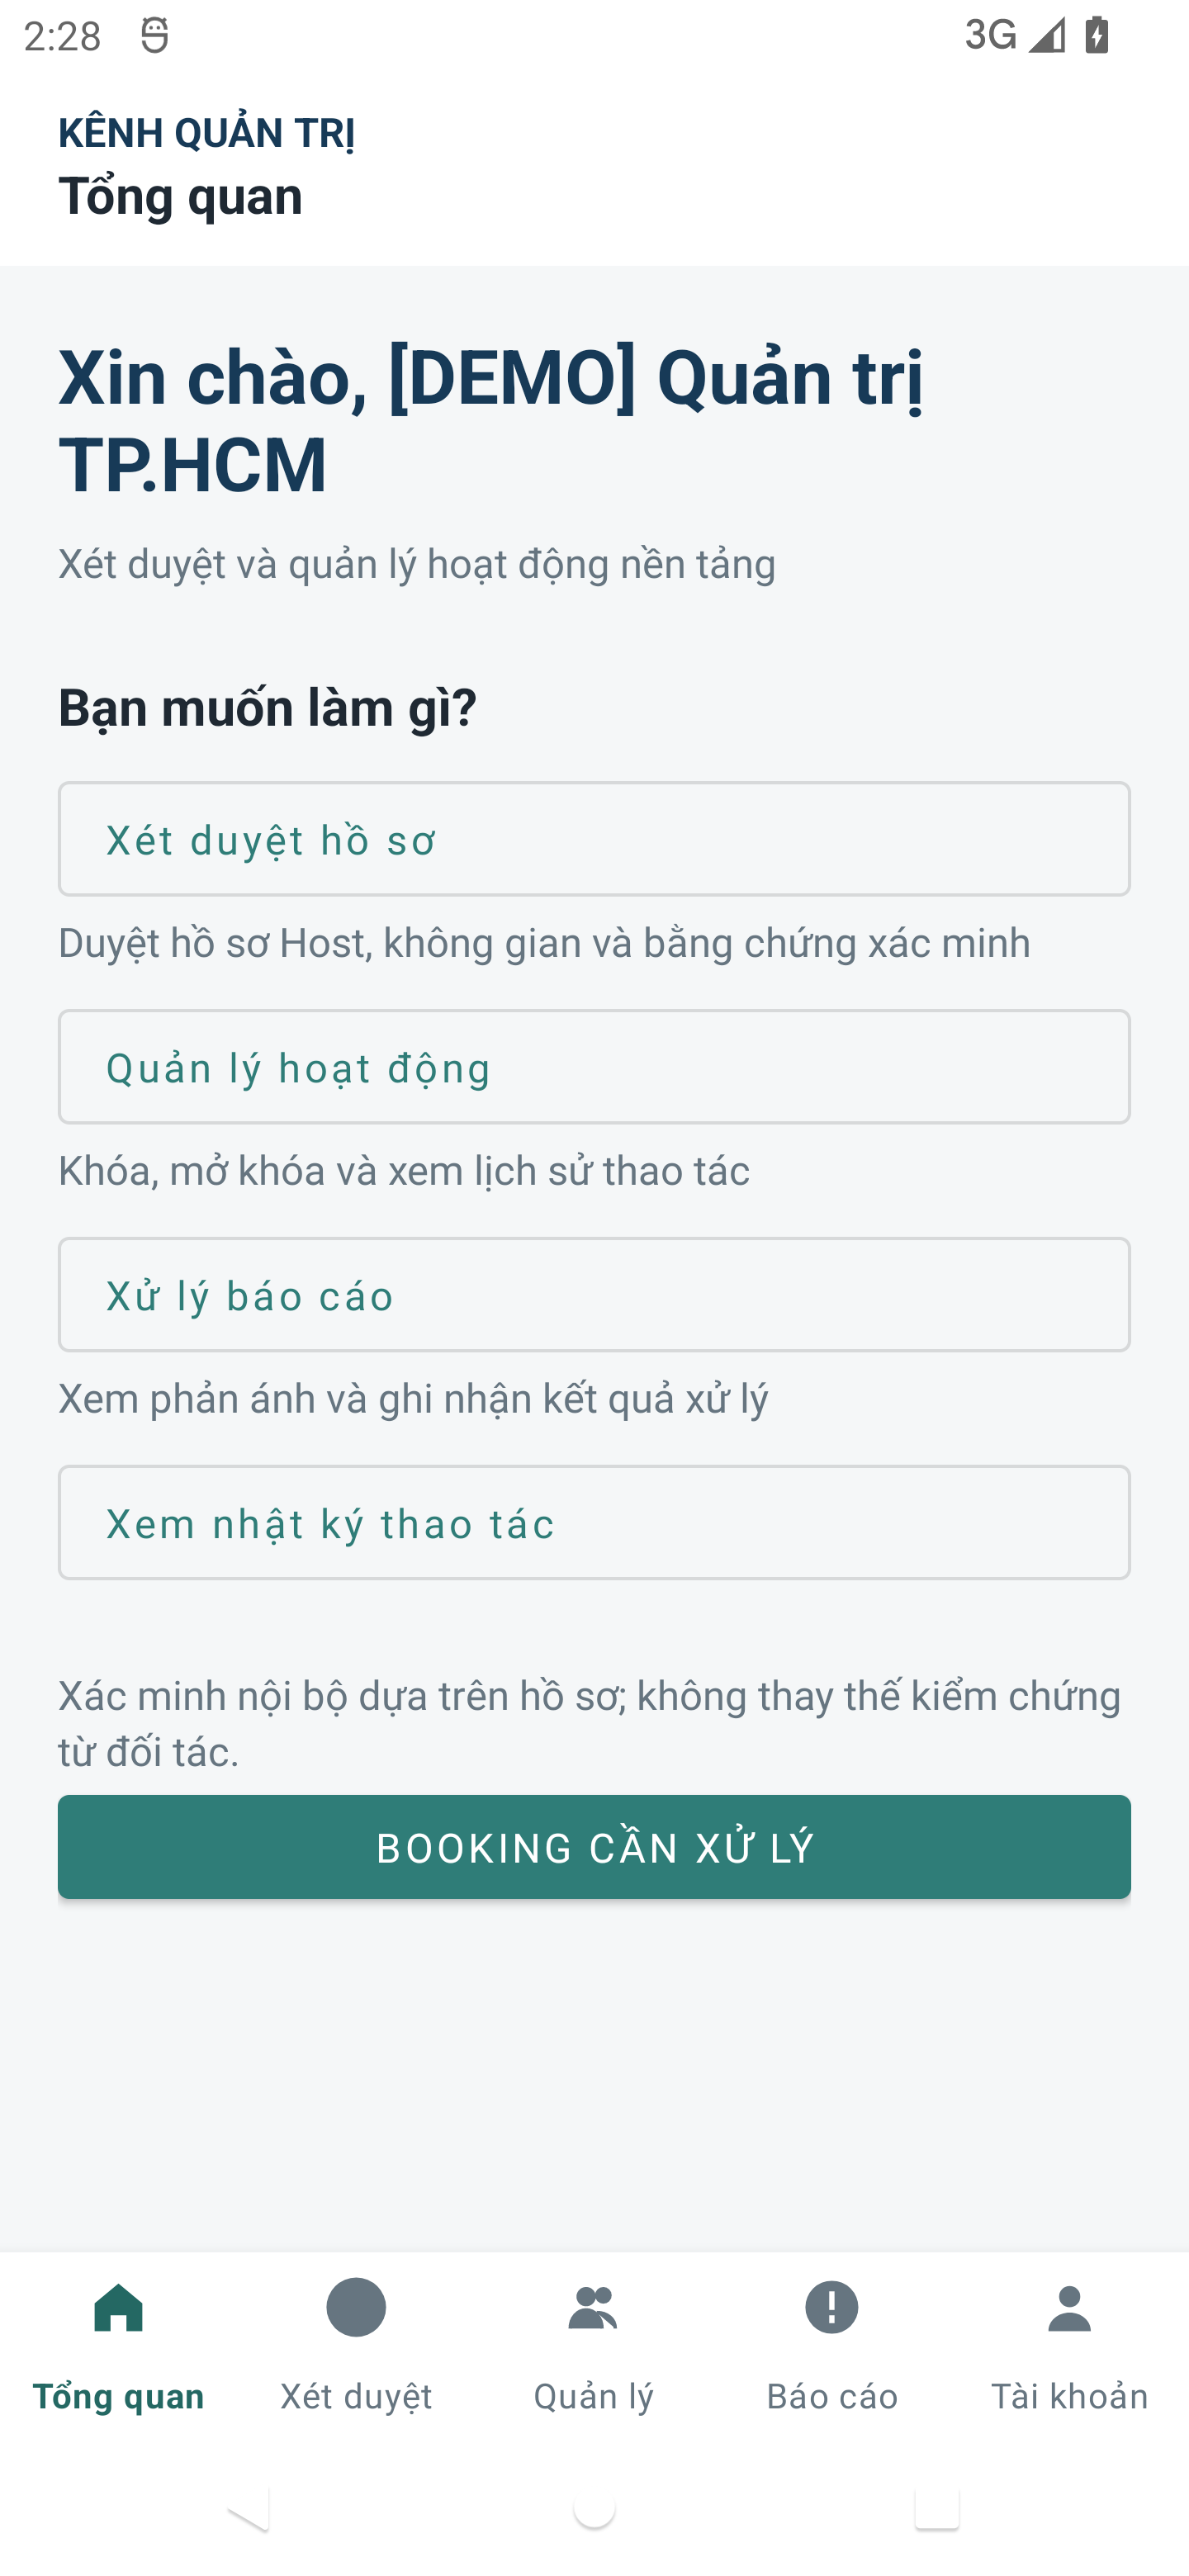
\includegraphics[width=\linewidth]{chapter5/admin-overview.png}\\[-1mm]
{\small (a) Tổng quan quản trị}
\end{minipage}\hspace{0.05\linewidth}%
\begin{minipage}[t]{0.40\linewidth}\centering
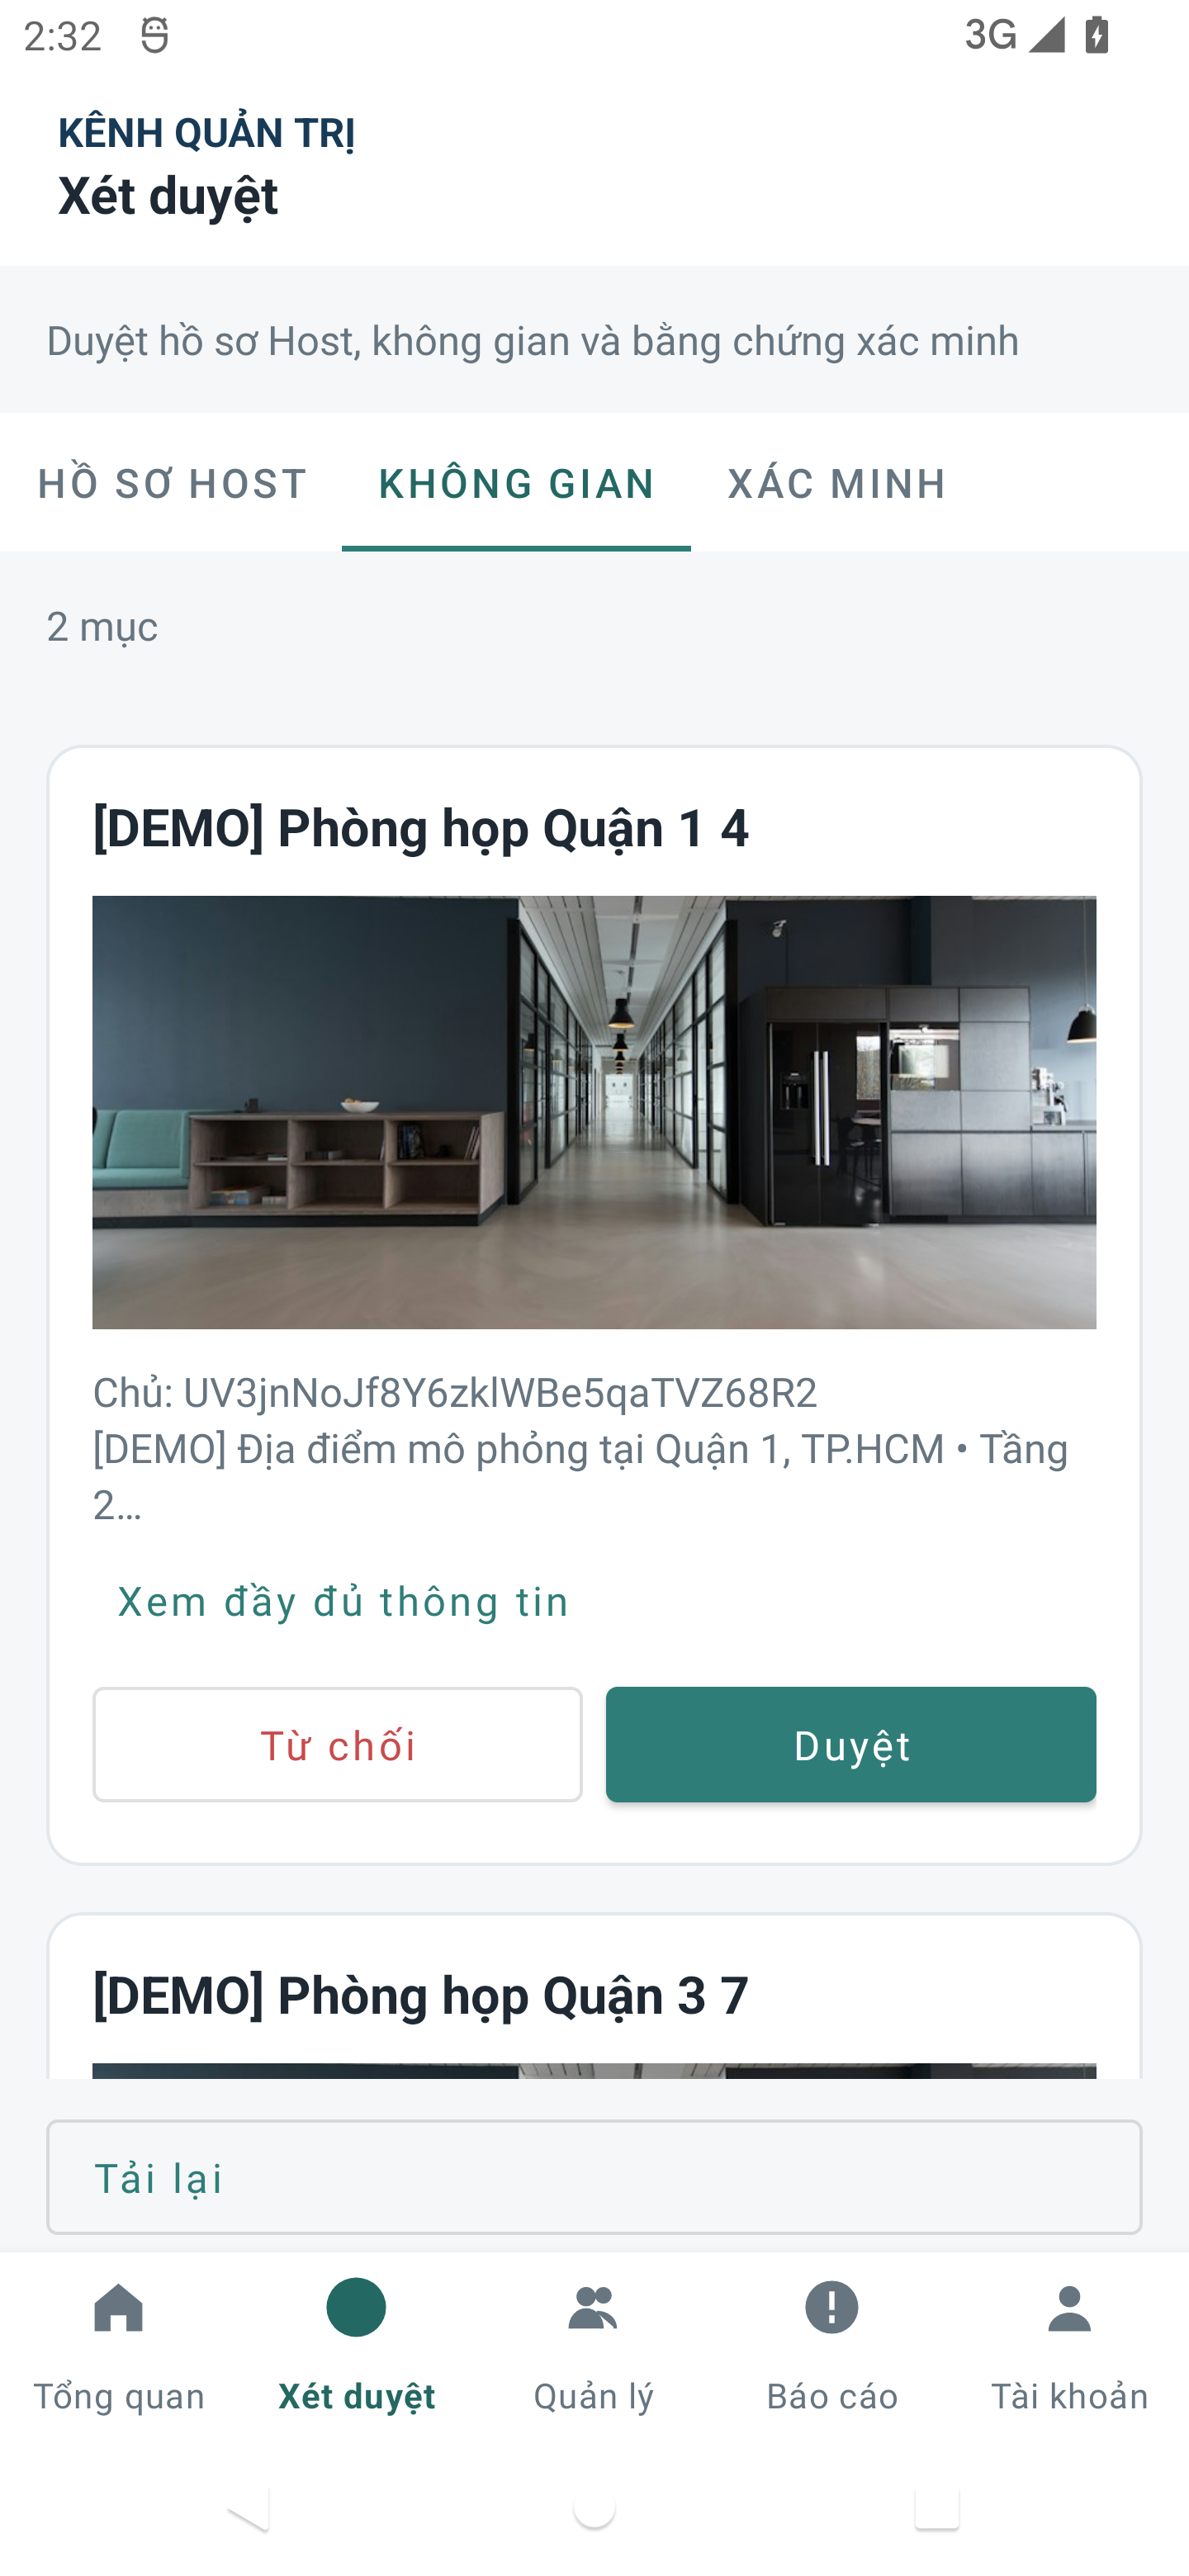
\includegraphics[width=\linewidth]{chapter5/admin-room-review.png}\\[-1mm]
{\small (b) Hàng đợi xét duyệt phòng}
\end{minipage}
\caption{Các màn hình tổng quan và xét duyệt tin đăng của Admin}
\label{fig:admin-overview-review}
\end{figure}}{}

Minh chứng vị trí và hình ảnh được đọc từ \texttt{propertyVerifications}, phân biệt với đơn xin quyền Host. Admin mở tệp ảnh hoặc PDF trong màn xem minh chứng, sau đó gửi kết quả xét duyệt cùng ghi chú. Repository ghi người xử lý, thời điểm và phương thức ADMIN\_REVIEWED; thông tin xác minh liên quan được cập nhật theo đối tượng phòng hoặc tòa nhà. Quy trình xác minh được thực hiện thủ công trên minh chứng DEMO, chưa có đối tác xác thực tự động.

Nhóm quản lý cho phép khóa hoặc mở khóa Host, đình chỉ hoặc gỡ đình chỉ phòng. Trạng thái tài khoản được đồng bộ với bản chiếu Host công khai; các quyền nhận đặt mới và thao tác nghiệp vụ được kiểm lại khi sử dụng. Lịch sử booking không bị xóa khi tài khoản bị khóa. Với báo cáo vi phạm, Admin đọc nội dung, phản hồi của Host và booking liên quan, rồi nhập kết luận. Kết quả được lưu thành RESOLVED hoặc DISMISSED; hành động xử lý có thể là ghi kết luận, đình chỉ phòng hoặc khóa Host.

Các booking cần can thiệp được mở ở màn hình riêng trong Hình~\ref{fig:admin-reports-bookings}. Admin xử lý từng trường hợp, không hủy đồng loạt theo trạng thái Host. Những thao tác như hủy booking chưa check-in của Host bị khóa, kết thúc lượt đang sử dụng do sự cố hoặc xác minh lại việc sử dụng đều yêu cầu căn cứ phù hợp và lý do. BookingRepository kiểm quyền và trạng thái hiện tại, cập nhật lịch khi cần nhả giữ chỗ, đồng thời ghi audit. Việc khép vụ việc không được tự đổi số tiền thành đã thu hoặc đã hoàn.

\IfFileExists{Resources/chapter5/admin-reports.png}{%
Hình~\ref{fig:admin-reports-bookings}(a) trình bày các báo cáo đang chờ xử lý. Admin mở nội dung đầy đủ rồi chọn bỏ qua hoặc ghi nhận kết quả, kèm kết luận và hành động phù hợp. Màn booking ở Hình~\ref{fig:admin-reports-bookings}(b) hiển thị mã đặt chỗ, Host, kỳ thuê và trạng thái của từng lượt. Các thao tác can thiệp được áp dụng cho từng booking sau khi kiểm tra điều kiện, giữ lại lịch sử và lý do xử lý.
\begin{figure}[H]
\centering
\begin{minipage}[t]{0.40\linewidth}\centering
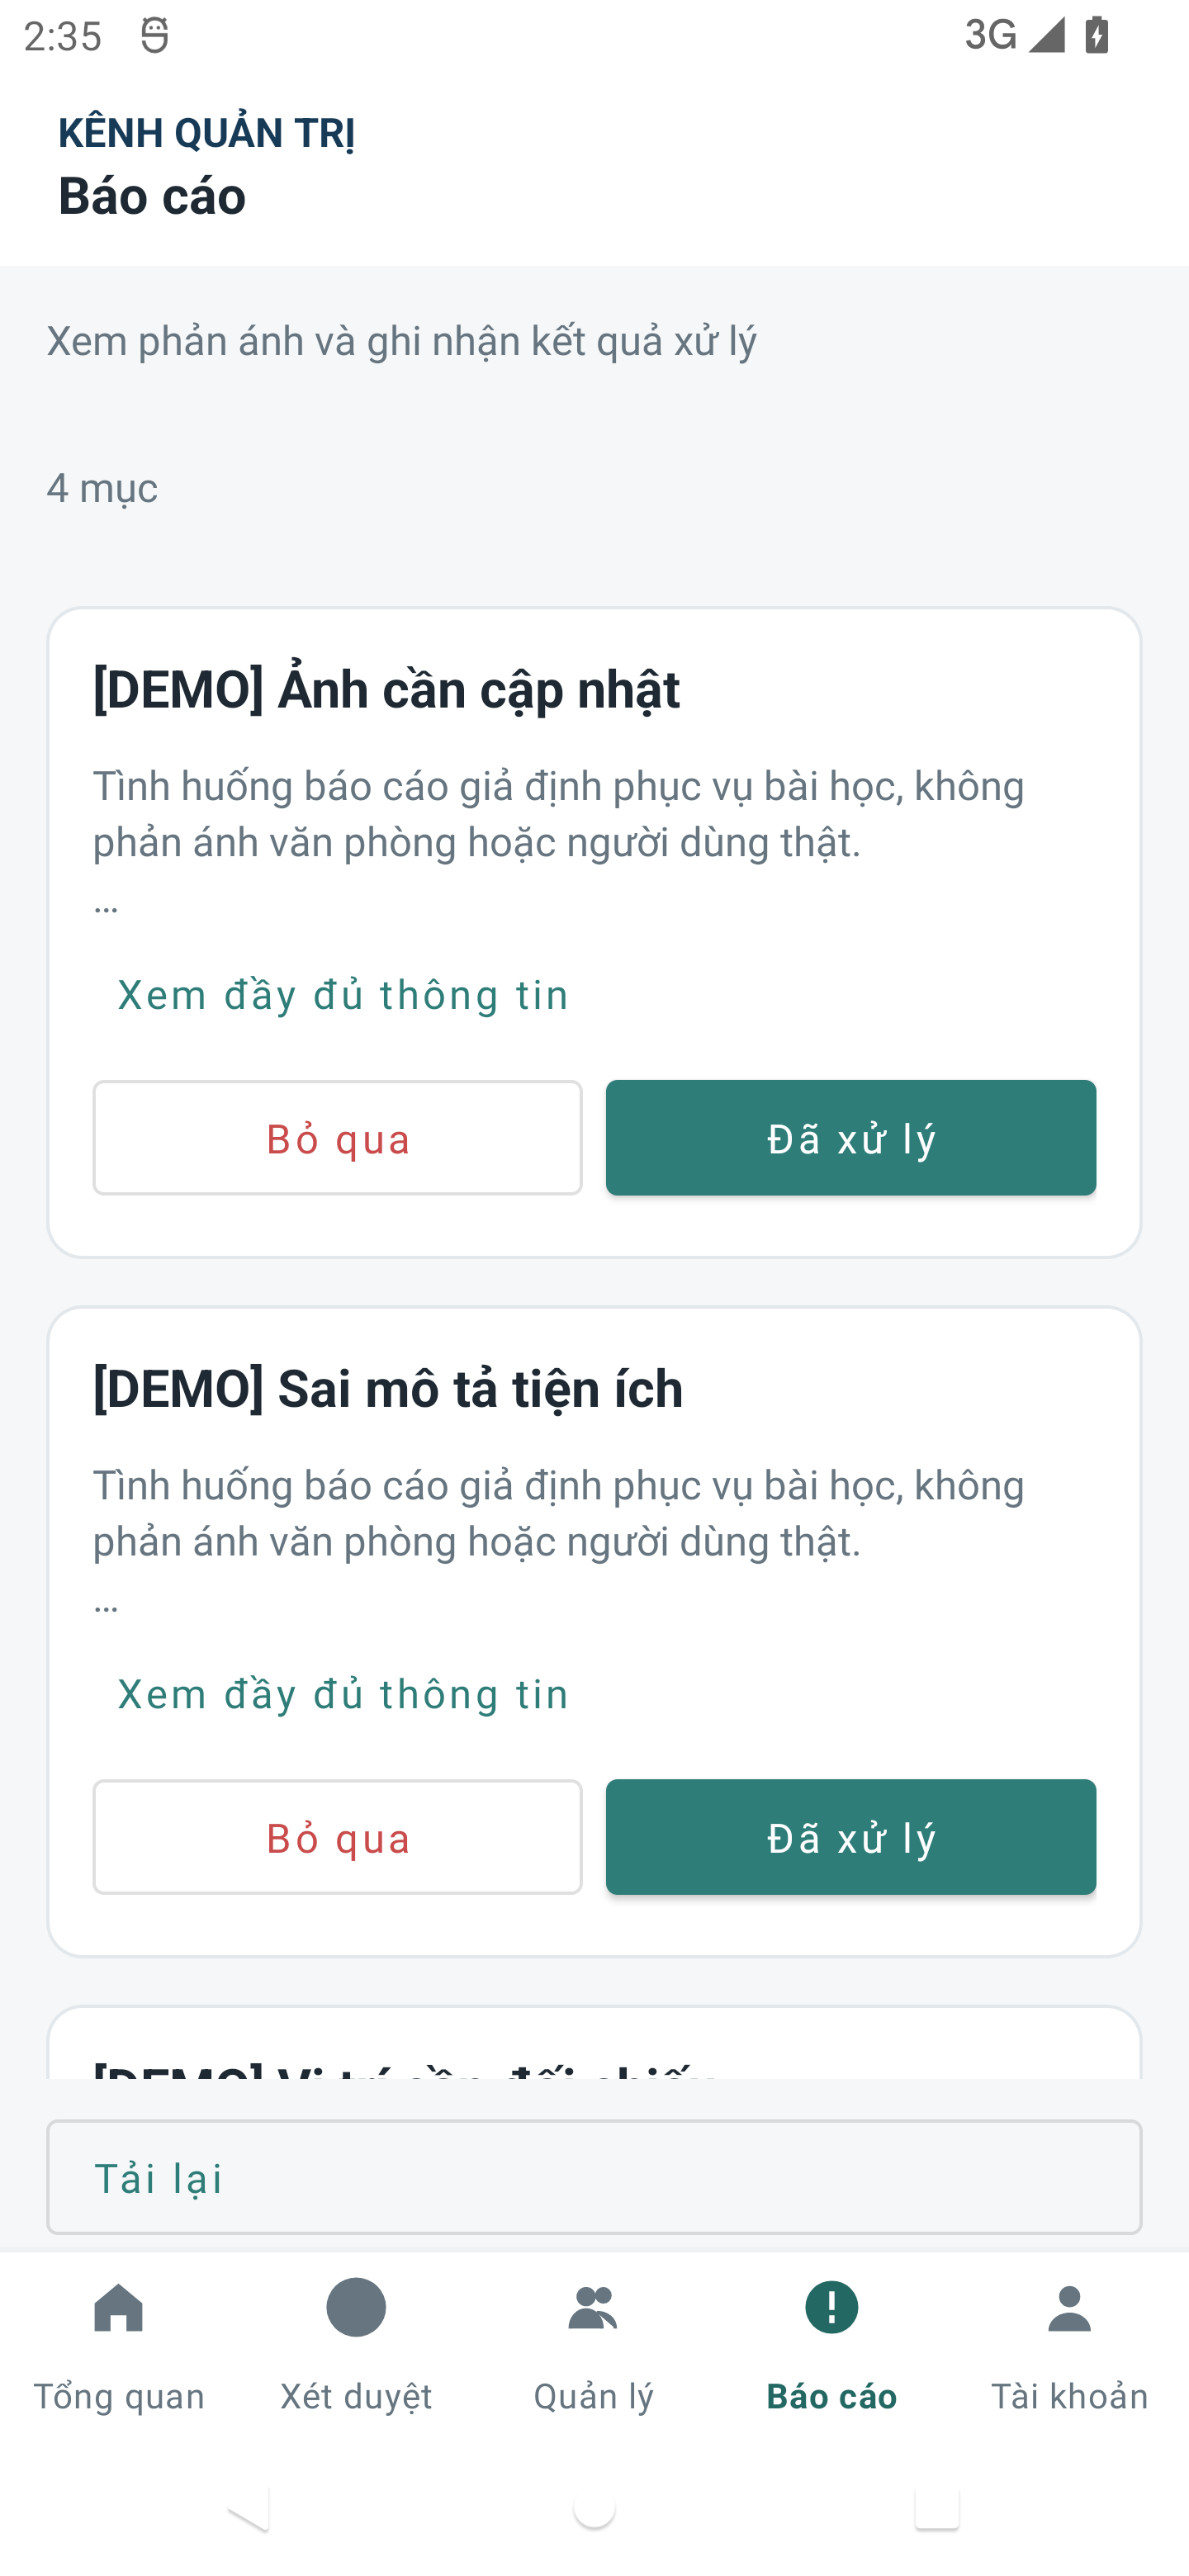
\includegraphics[width=\linewidth]{chapter5/admin-reports.png}\\[-1mm]
{\small (a) Báo cáo cần xử lý}
\end{minipage}\hspace{0.05\linewidth}%
\begin{minipage}[t]{0.40\linewidth}\centering
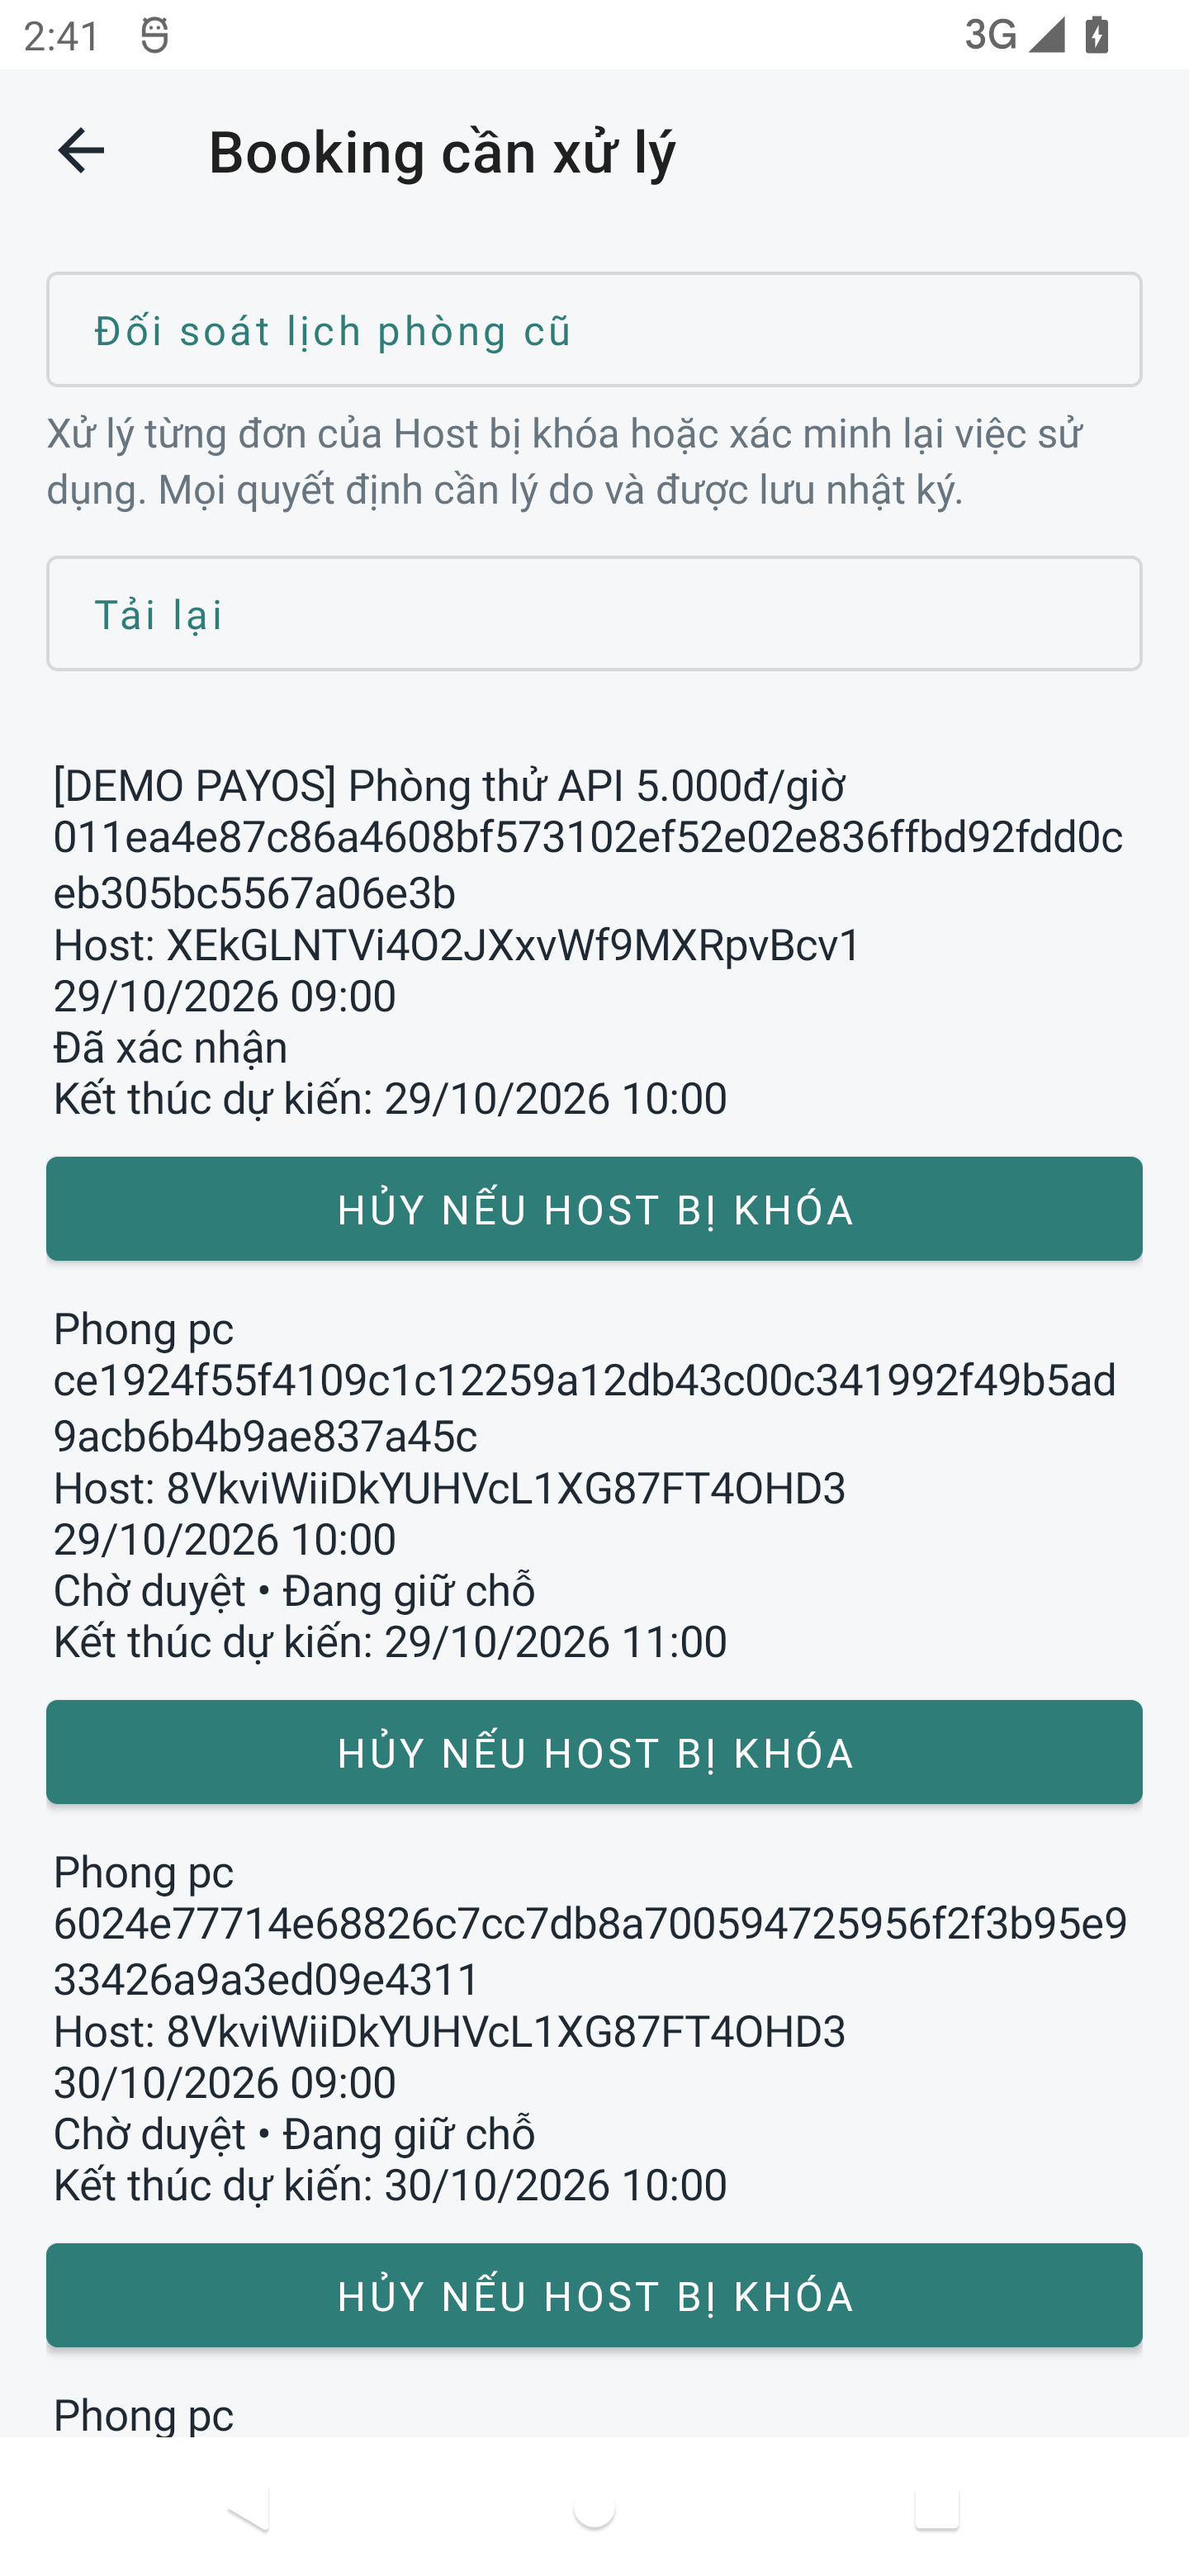
\includegraphics[width=\linewidth]{chapter5/admin-booking-cases.png}\\[-1mm]
{\small (b) Can thiệp từng booking}
\end{minipage}
\caption{Giao diện xử lý báo cáo và booking ngoại lệ}
\label{fig:admin-reports-bookings}
\end{figure}}{}

Màn đối soát lịch kiểm tra số booking còn giữ chỗ của một phòng và các khóa lịch tương ứng trước khi cập nhật bộ đếm. Chức năng này phục vụ trường hợp dữ liệu cũ cần đối chiếu, không tạo thêm phòng hoặc thay đổi hình thức thuê. Nhóm nhật ký đọc \texttt{auditLogs} để hiển thị người thực hiện, đối tượng, hành động và lý do theo thời gian. Hình~\ref{fig:admin-application-evidence} và Hình~\ref{fig:admin-host-audit} bổ sung các hàng đợi xét duyệt và dấu vết xử lý tương ứng.

\IfFileExists{Resources/chapter5/admin-applications.png}{%
Hàng đợi trong Hình~\ref{fig:admin-application-evidence}(a) cung cấp tên, thông tin liên hệ và mô tả hồ sơ xin quyền Host. Admin mở nội dung đầy đủ và tệp giấy tờ trước khi quyết định cấp quyền. Hình~\ref{fig:admin-application-evidence}(b) là hàng đợi minh chứng vị trí và ảnh, hiển thị phòng hoặc tòa nhà cần đối chiếu. Hai hàng đợi phục vụ hai quyết định độc lập: cấp quyền Host và xét duyệt minh chứng không gian.
\begin{figure}[H]
\centering
\begin{minipage}[t]{0.40\linewidth}\centering
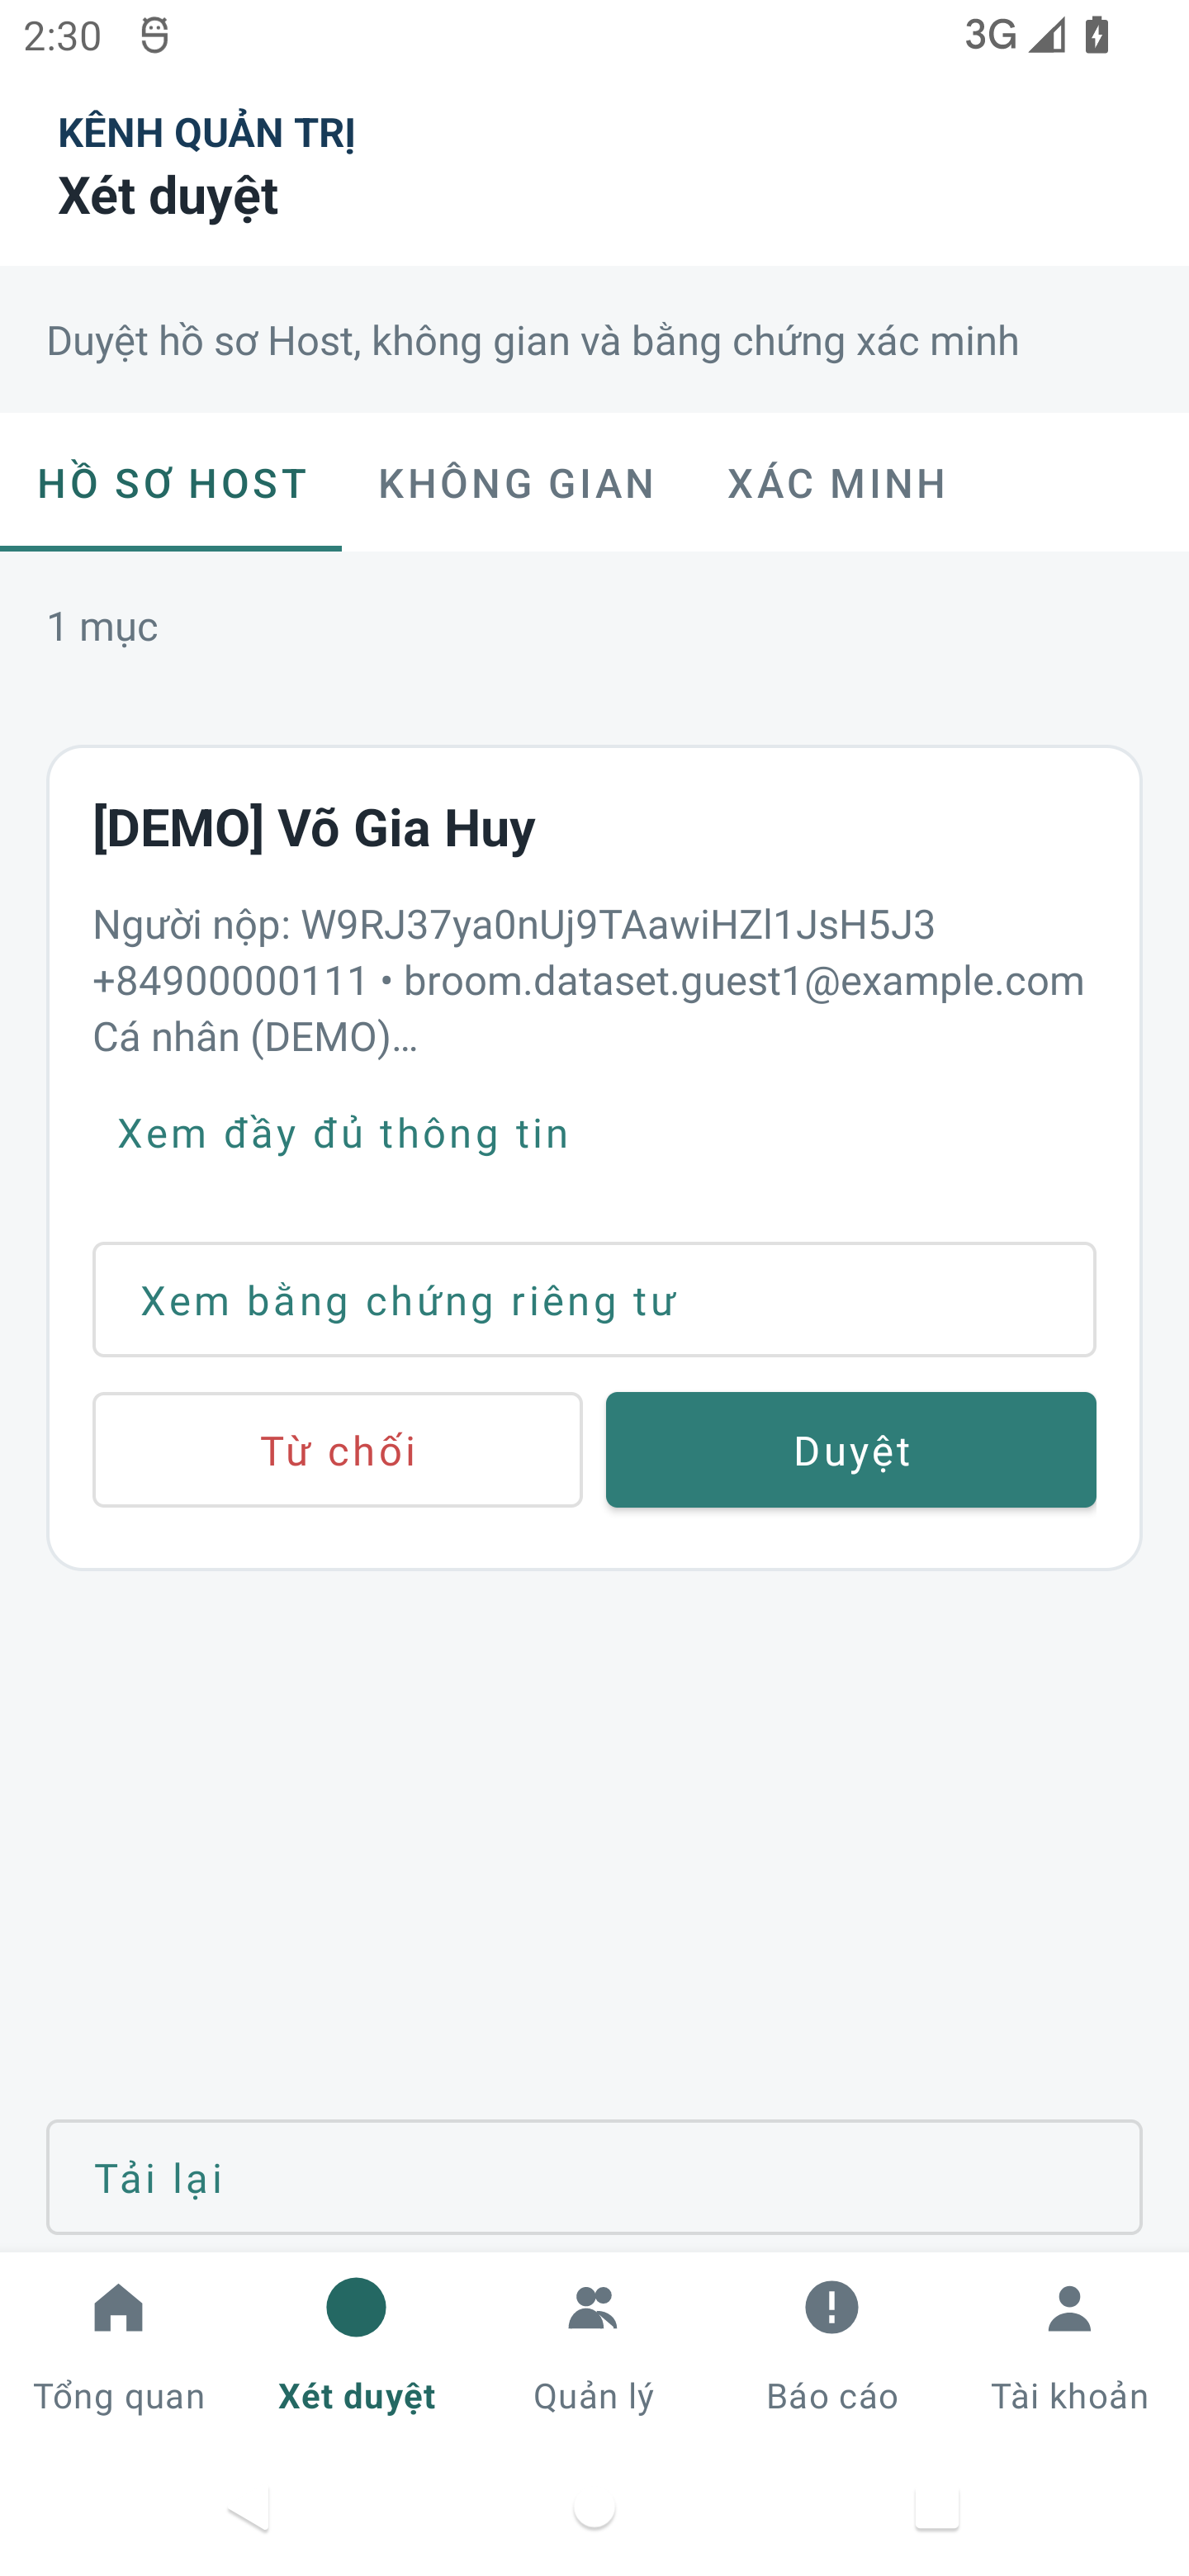
\includegraphics[width=\linewidth]{chapter5/admin-applications.png}\\[-1mm]
{\small (a) Hồ sơ xin quyền Host}
\end{minipage}\hspace{0.05\linewidth}%
\begin{minipage}[t]{0.40\linewidth}\centering
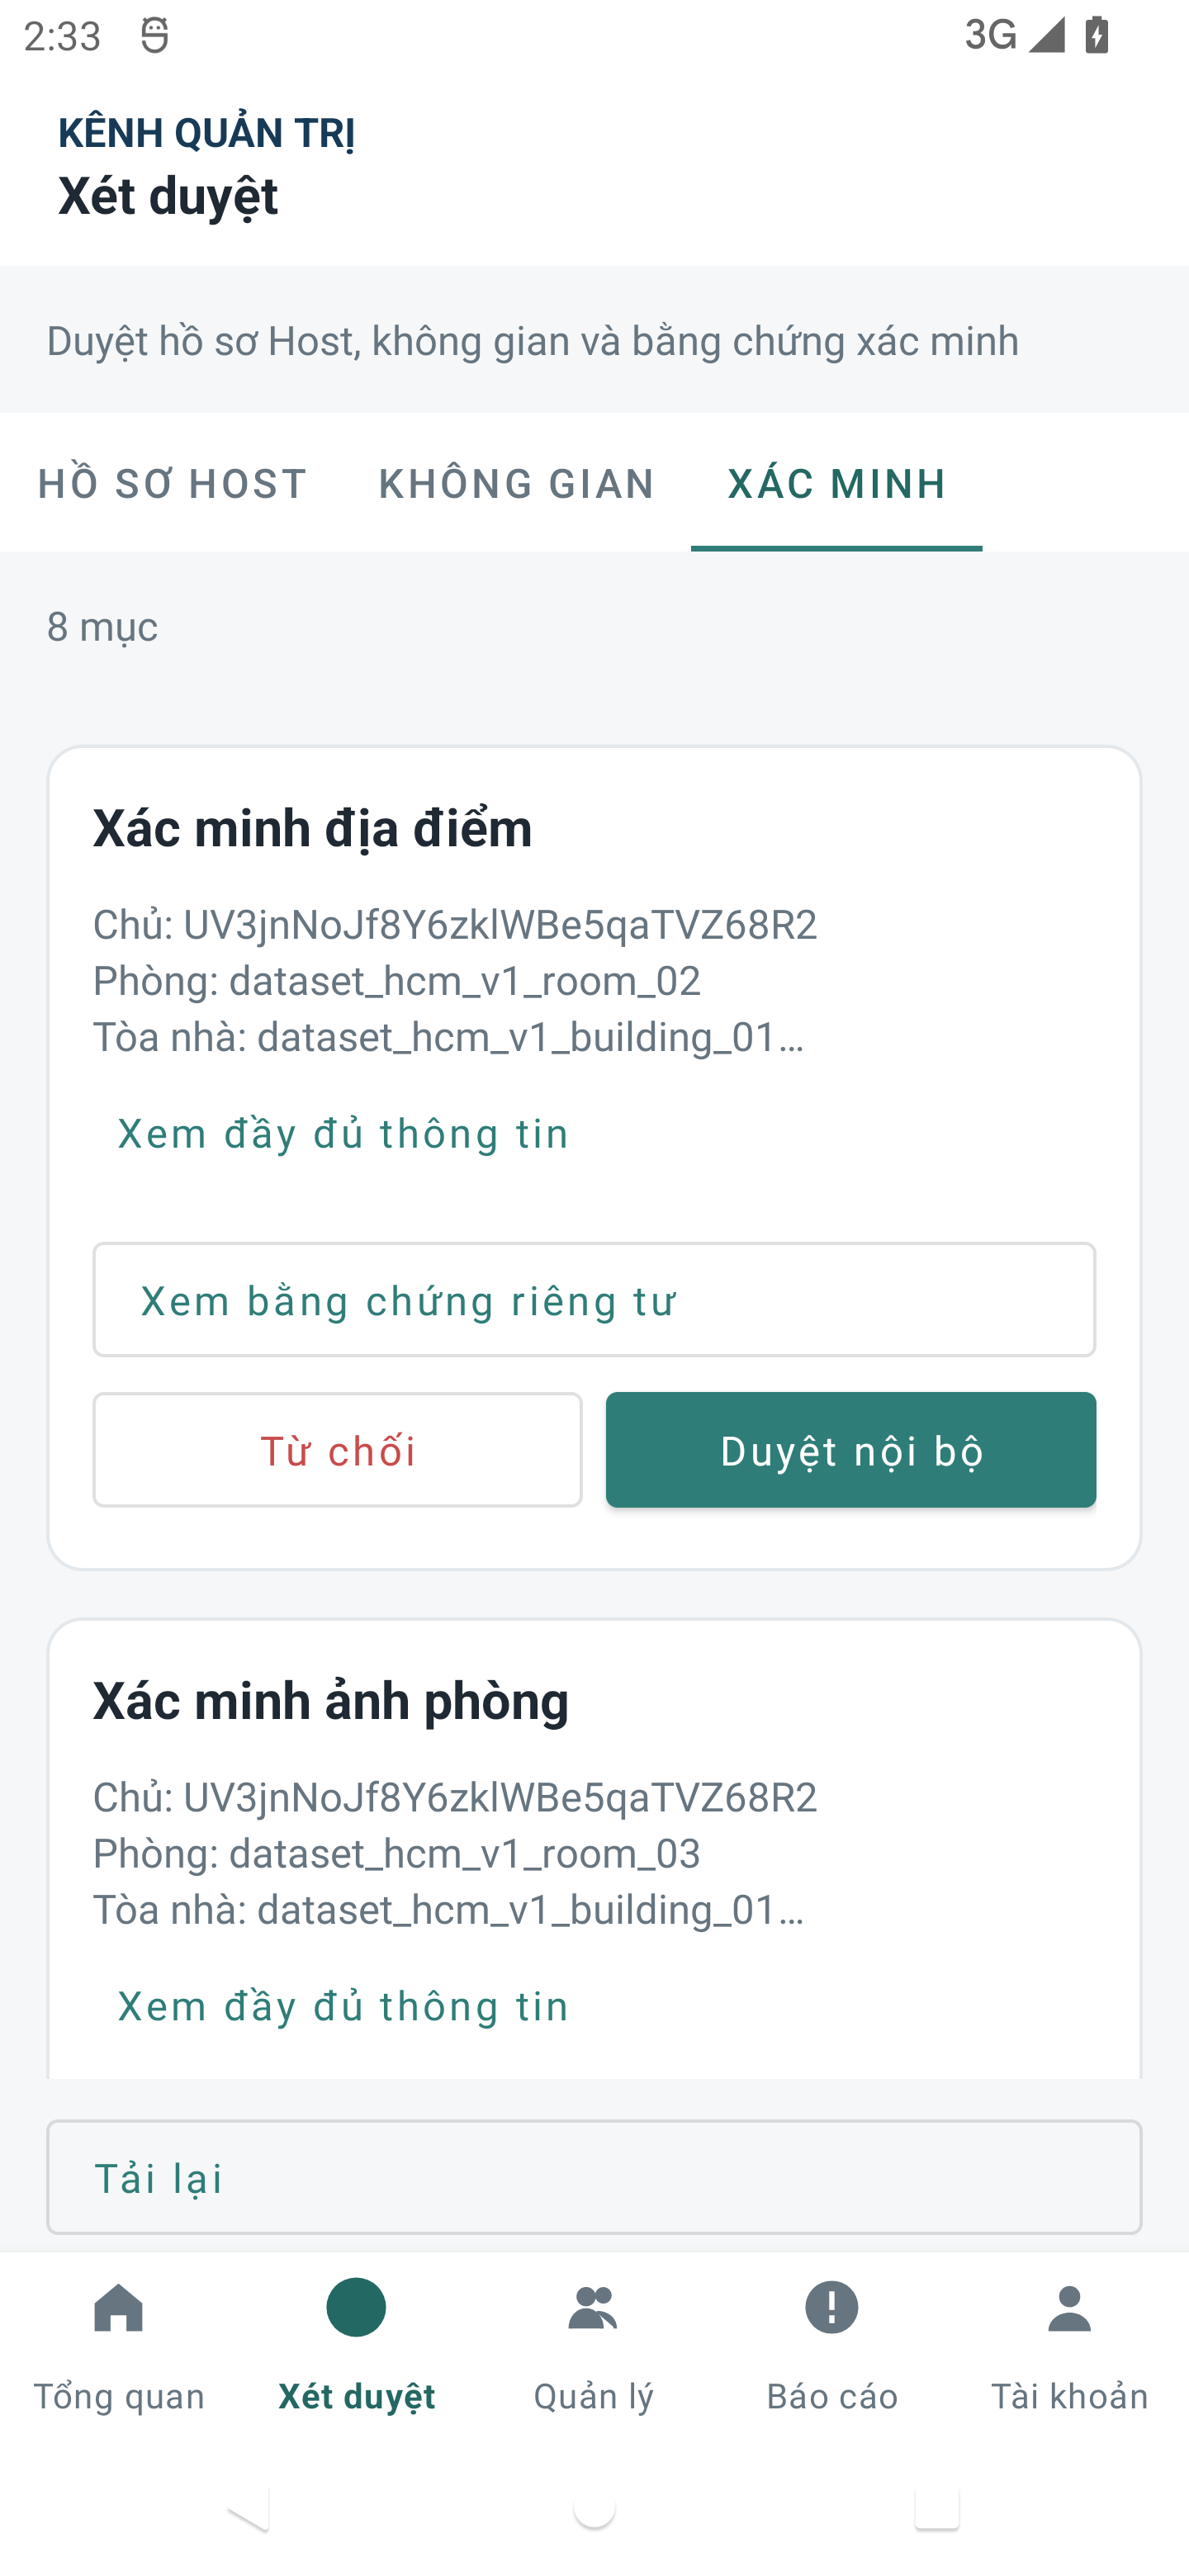
\includegraphics[width=\linewidth]{chapter5/admin-verifications.png}\\[-1mm]
{\small (b) Minh chứng vị trí và ảnh}
\end{minipage}
\caption{Hàng đợi hồ sơ Host và minh chứng không gian}
\label{fig:admin-application-evidence}
\end{figure}}{}

\IfFileExists{Resources/chapter5/admin-hosts.png}{%
Hình~\ref{fig:admin-host-audit}(a) hiển thị tài khoản Host cùng trạng thái hoạt động và thao tác khóa hoặc mở khóa tương ứng. Lý do xử lý được lưu để đối chiếu khi quản lý quyền nhận đặt mới. Nhật ký ở Hình~\ref{fig:admin-host-audit}(b) trình bày hành động, người thực hiện, đối tượng và thay đổi trạng thái theo thời gian. Admin có thể mở nội dung đầy đủ để kiểm tra một quyết định cụ thể; danh sách được giới hạn ở 100 thao tác mới nhất.
\begin{figure}[H]
\centering
\begin{minipage}[t]{0.40\linewidth}\centering
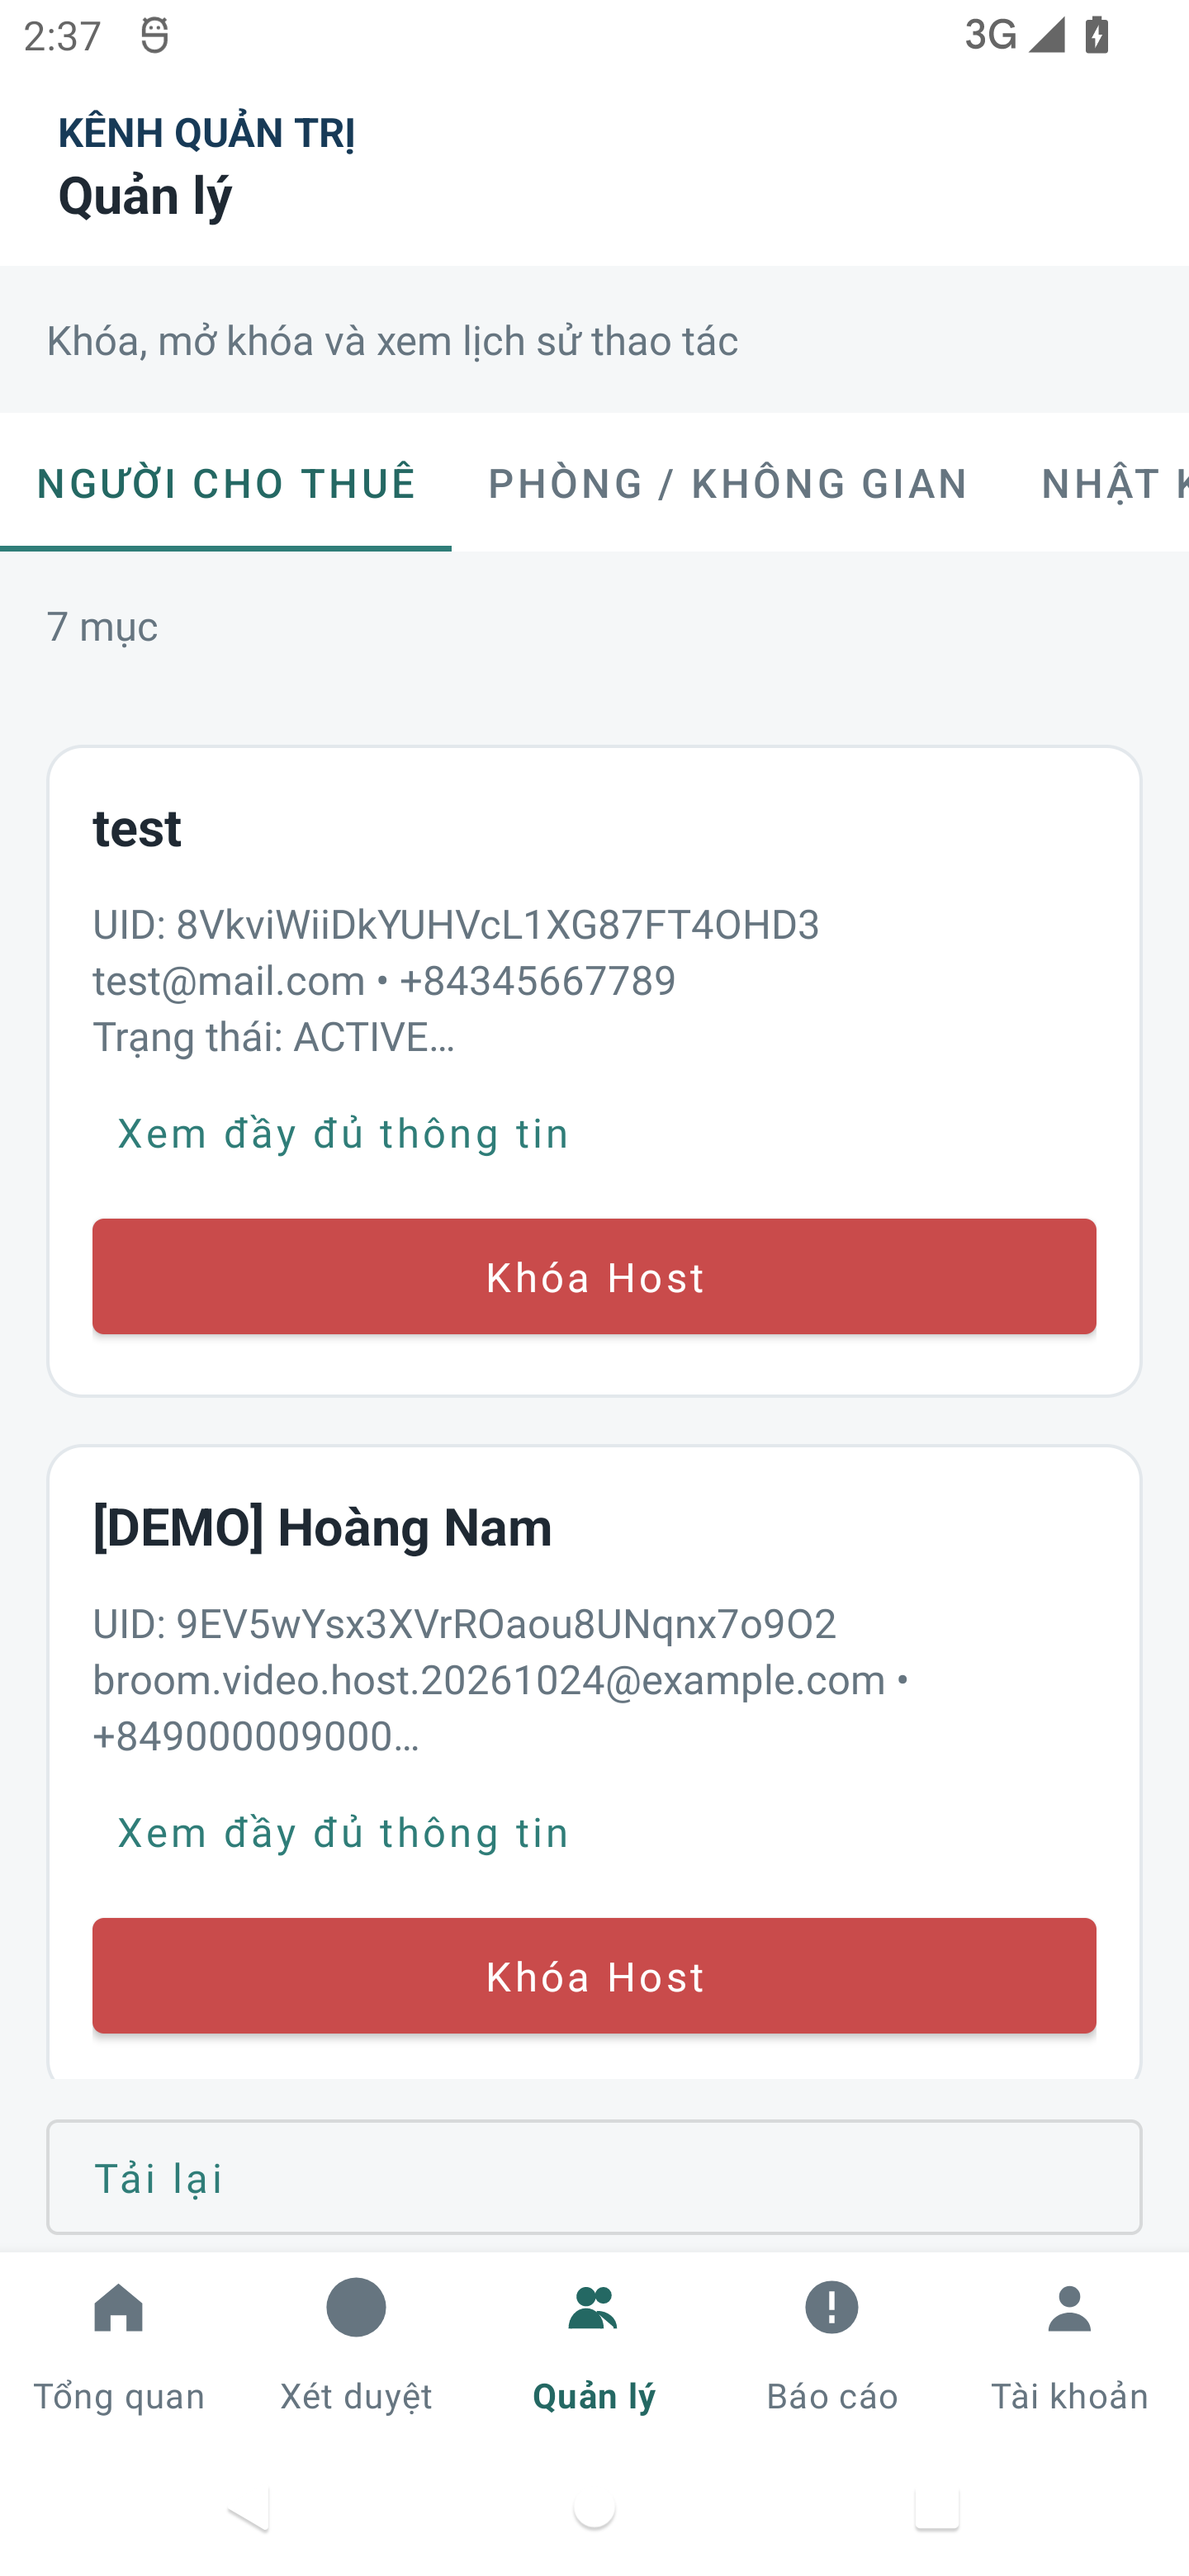
\includegraphics[width=\linewidth]{chapter5/admin-hosts.png}\\[-1mm]
{\small (a) Trạng thái Host}
\end{minipage}\hspace{0.05\linewidth}%
\begin{minipage}[t]{0.40\linewidth}\centering
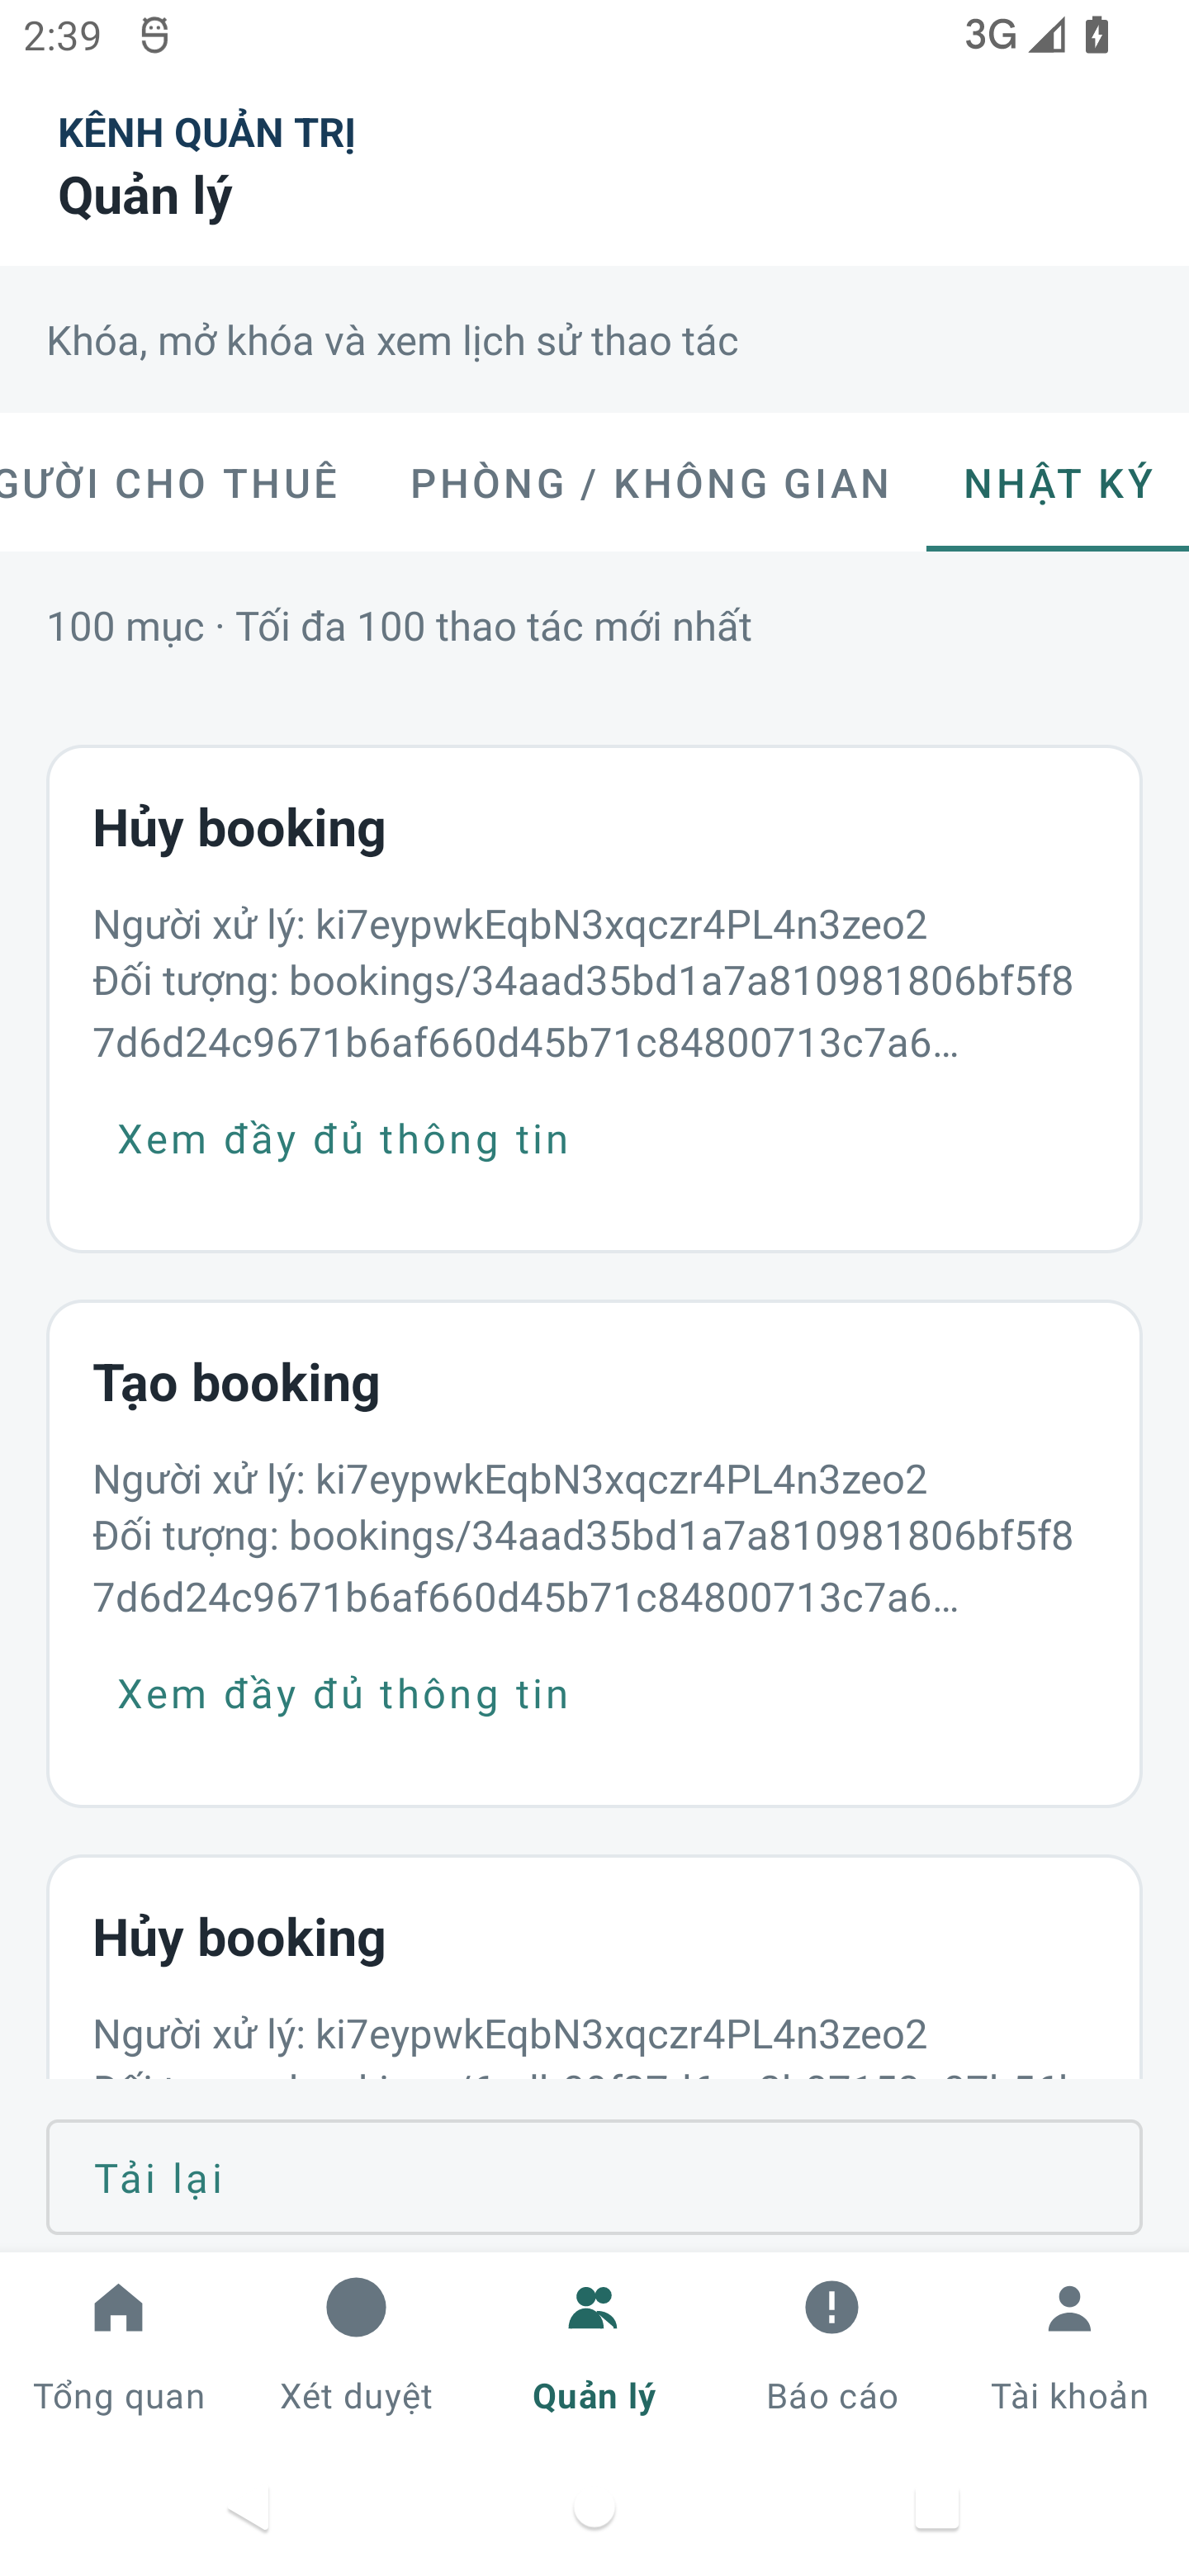
\includegraphics[width=\linewidth]{chapter5/admin-audit.png}\\[-1mm]
{\small (b) Nhật ký nghiệp vụ}
\end{minipage}
\caption{Giao diện quản lý Host và tra cứu nhật ký}
\label{fig:admin-host-audit}
\end{figure}}{}


\FloatBarrier
\subsection{Thích ứng giao diện và xử lý trạng thái}
\label{sec:application-responsive}
\subsubsection{Thích ứng khi xoay màn hình và thay đổi kích thước}
Android chọn các biến thể XML theo hướng màn hình và kích thước nhỏ nhất, gồm \texttt{layout-land} và \texttt{sw600dp}. Trên tablet ngang, Trang chủ chuyển vùng tìm kiếm sang cột bên trái và hiển thị phòng theo grid; kênh Host tách vùng chọn phòng/tòa nhà khỏi danh sách. Hình~\ref{fig:adaptive-user-host} minh họa hai bố cục này. Các vùng dữ liệu cuộn độc lập để nút và nội dung không bị thanh điều hướng che khuất.

\begin{figure}[H]\centering
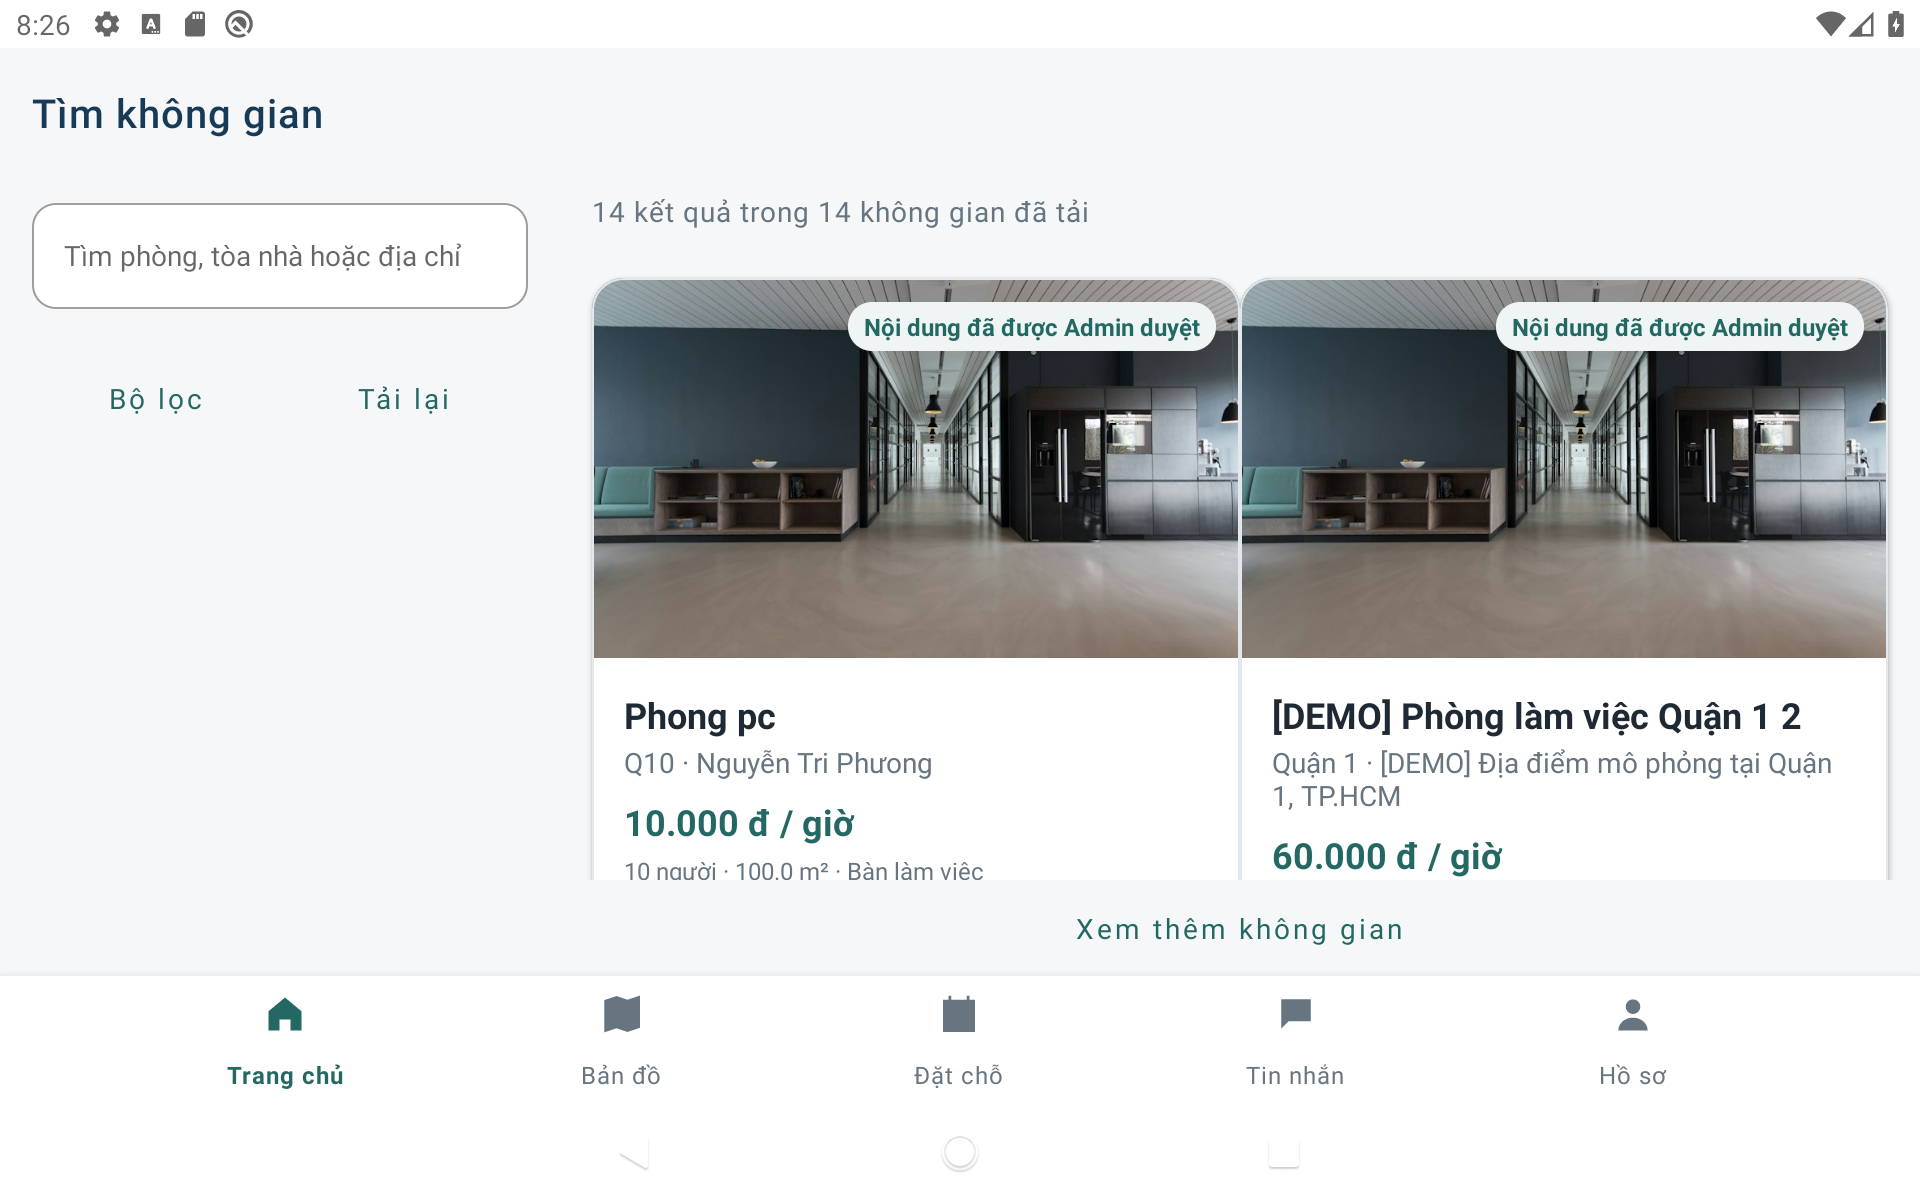
\includegraphics[width=0.94\linewidth]{chapter5/members/user-tablet-home-landscape.png}\\[-1mm]
{\small (a) Trang chủ ở chế độ thuê}
\par\medskip
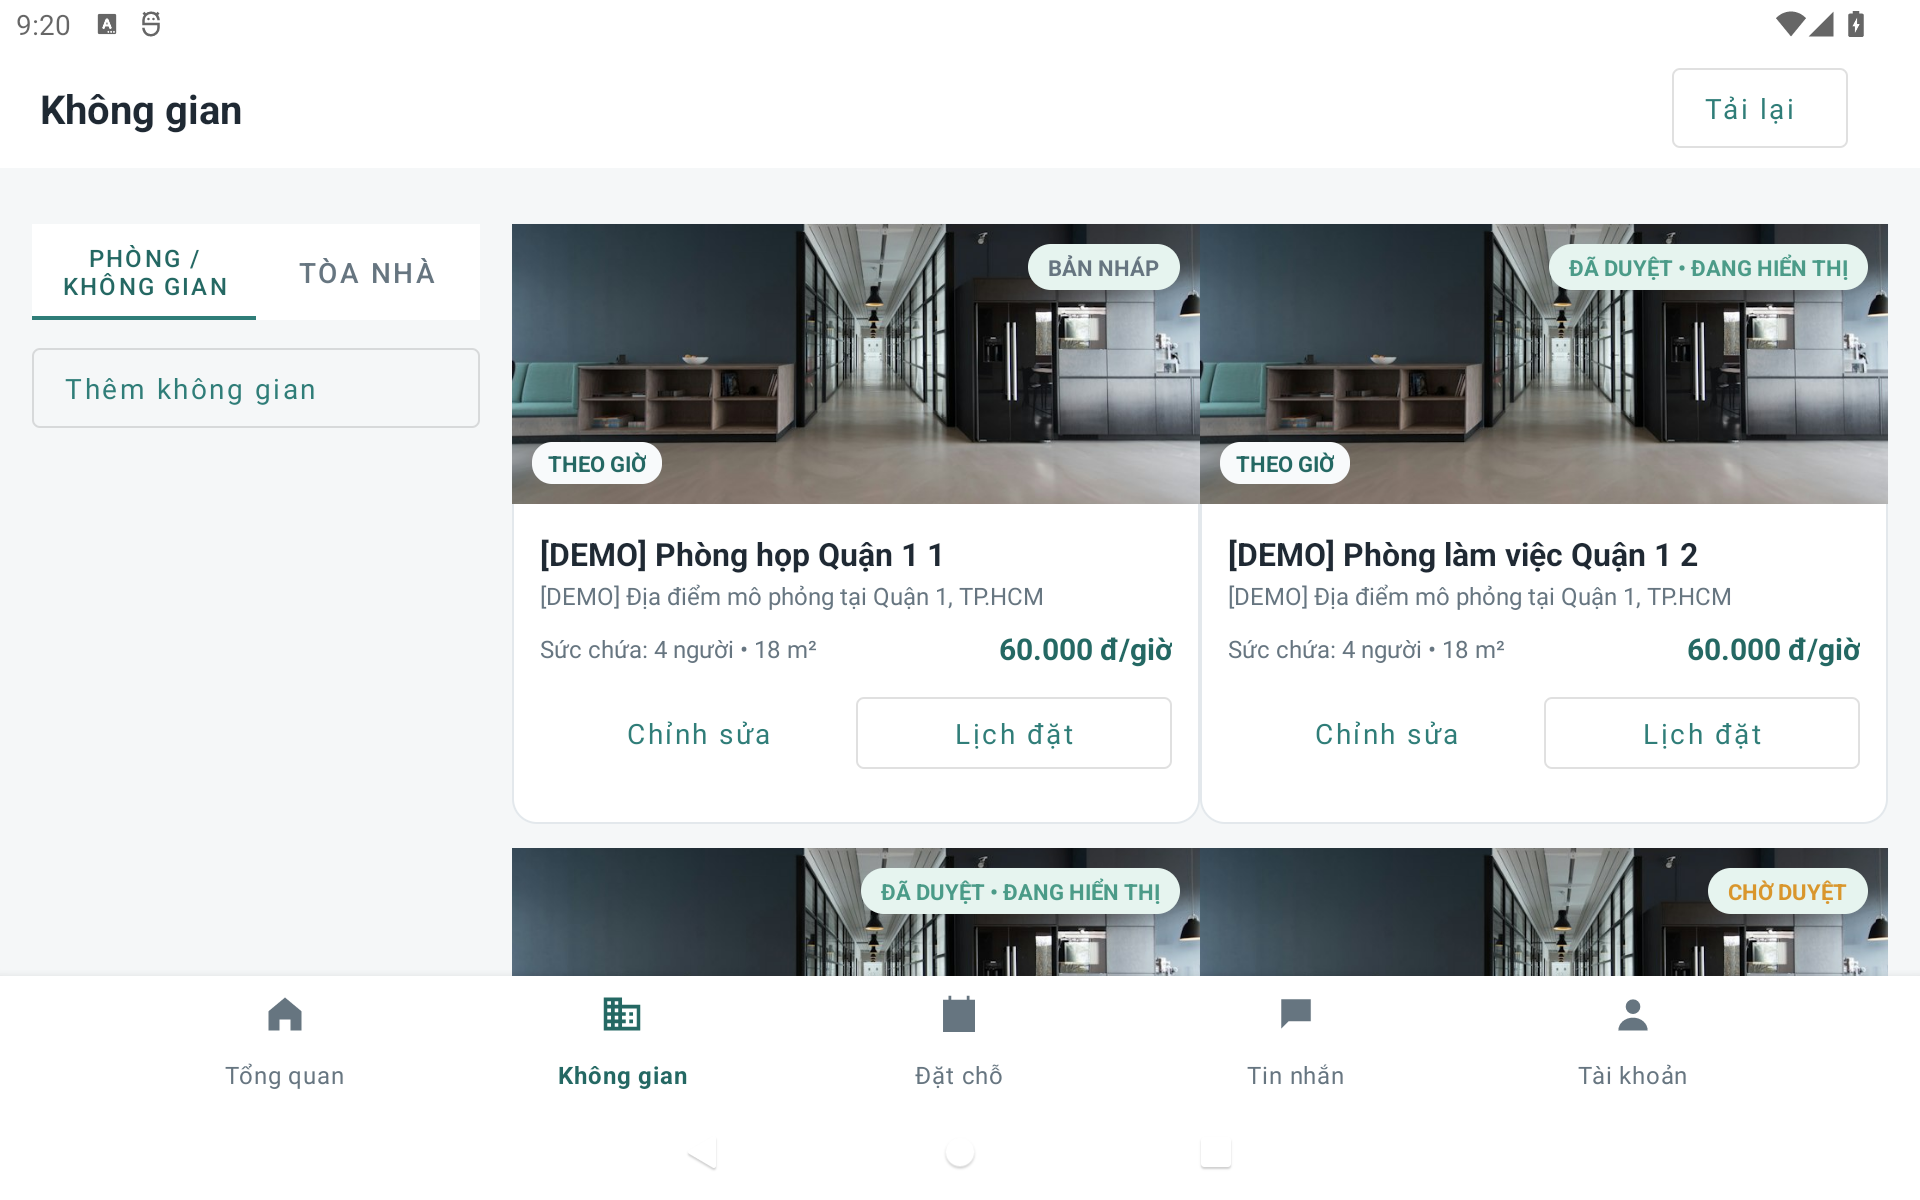
\includegraphics[width=0.94\linewidth]{chapter5/members/host-tablet-spaces-landscape.png}\\[-1mm]
{\small (b) Quản lý không gian của Host}
\caption{Bố cục hai vùng trên tablet Android ở chiều ngang}
\label{fig:adaptive-user-host}
\end{figure}

Activity lưu lựa chọn cần khôi phục, còn ViewModel duy trì dữ liệu qua thay đổi cấu hình \parencite{android_runtime_changes,android_resource_variants}. Khi xoay, tab hoặc bộ lọc đang chọn được phục hồi; màn bản đồ giữ điểm đến và tuyến đã nhận. Listener được quản lý theo vòng đời để tránh đăng ký lặp khi màn hình tái tạo.

\subsubsection{Xử lý trạng thái tải, rỗng, lỗi và quyền truy cập}
Giao diện phân biệt đang tải với danh sách rỗng, khóa thao tác gửi khi request chưa kết thúc và hiển thị lỗi kèm lựa chọn thử lại. Hình~\ref{fig:adaptive-admin} cho thấy kênh Admin đổi cách bố trí theo kích thước: điện thoại ngang giữ tab trên danh sách, tablet ngang đặt nhóm hồ sơ ở cột trái. Quyền xét duyệt vẫn được kiểm tra từ phiên và dữ liệu hiện tại, không thay đổi theo bố cục.

\begin{figure}[H]\centering
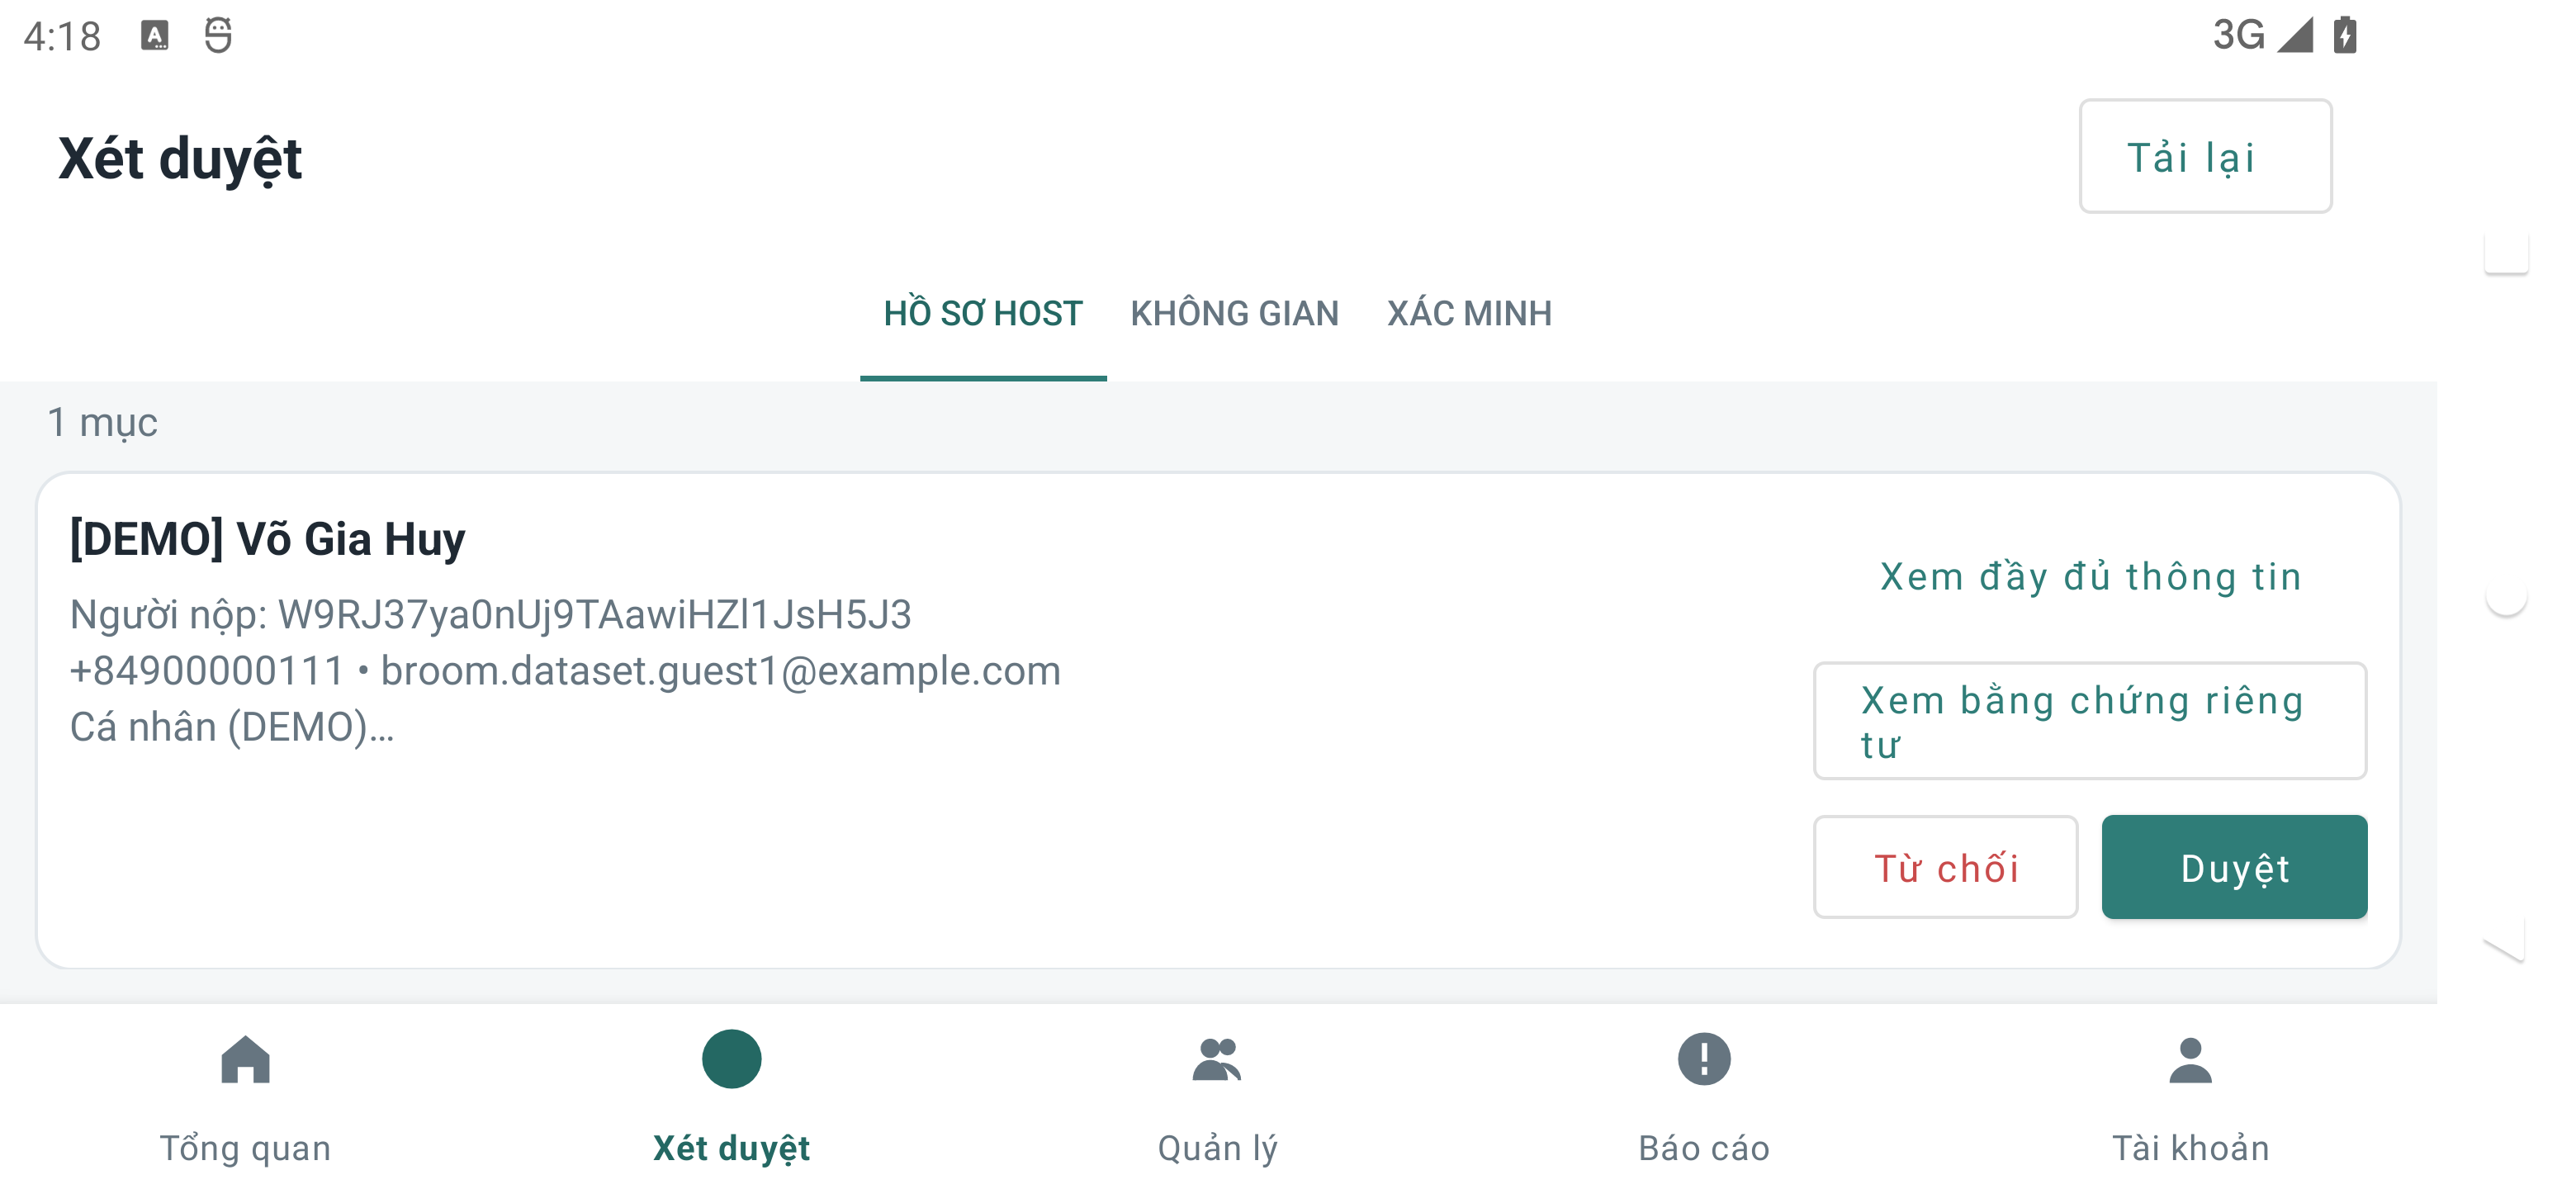
\includegraphics[width=0.94\linewidth]{chapter5/admin-phone-landscape.png}\\[-1mm]
{\small (a) Điện thoại ngang}
\par\medskip
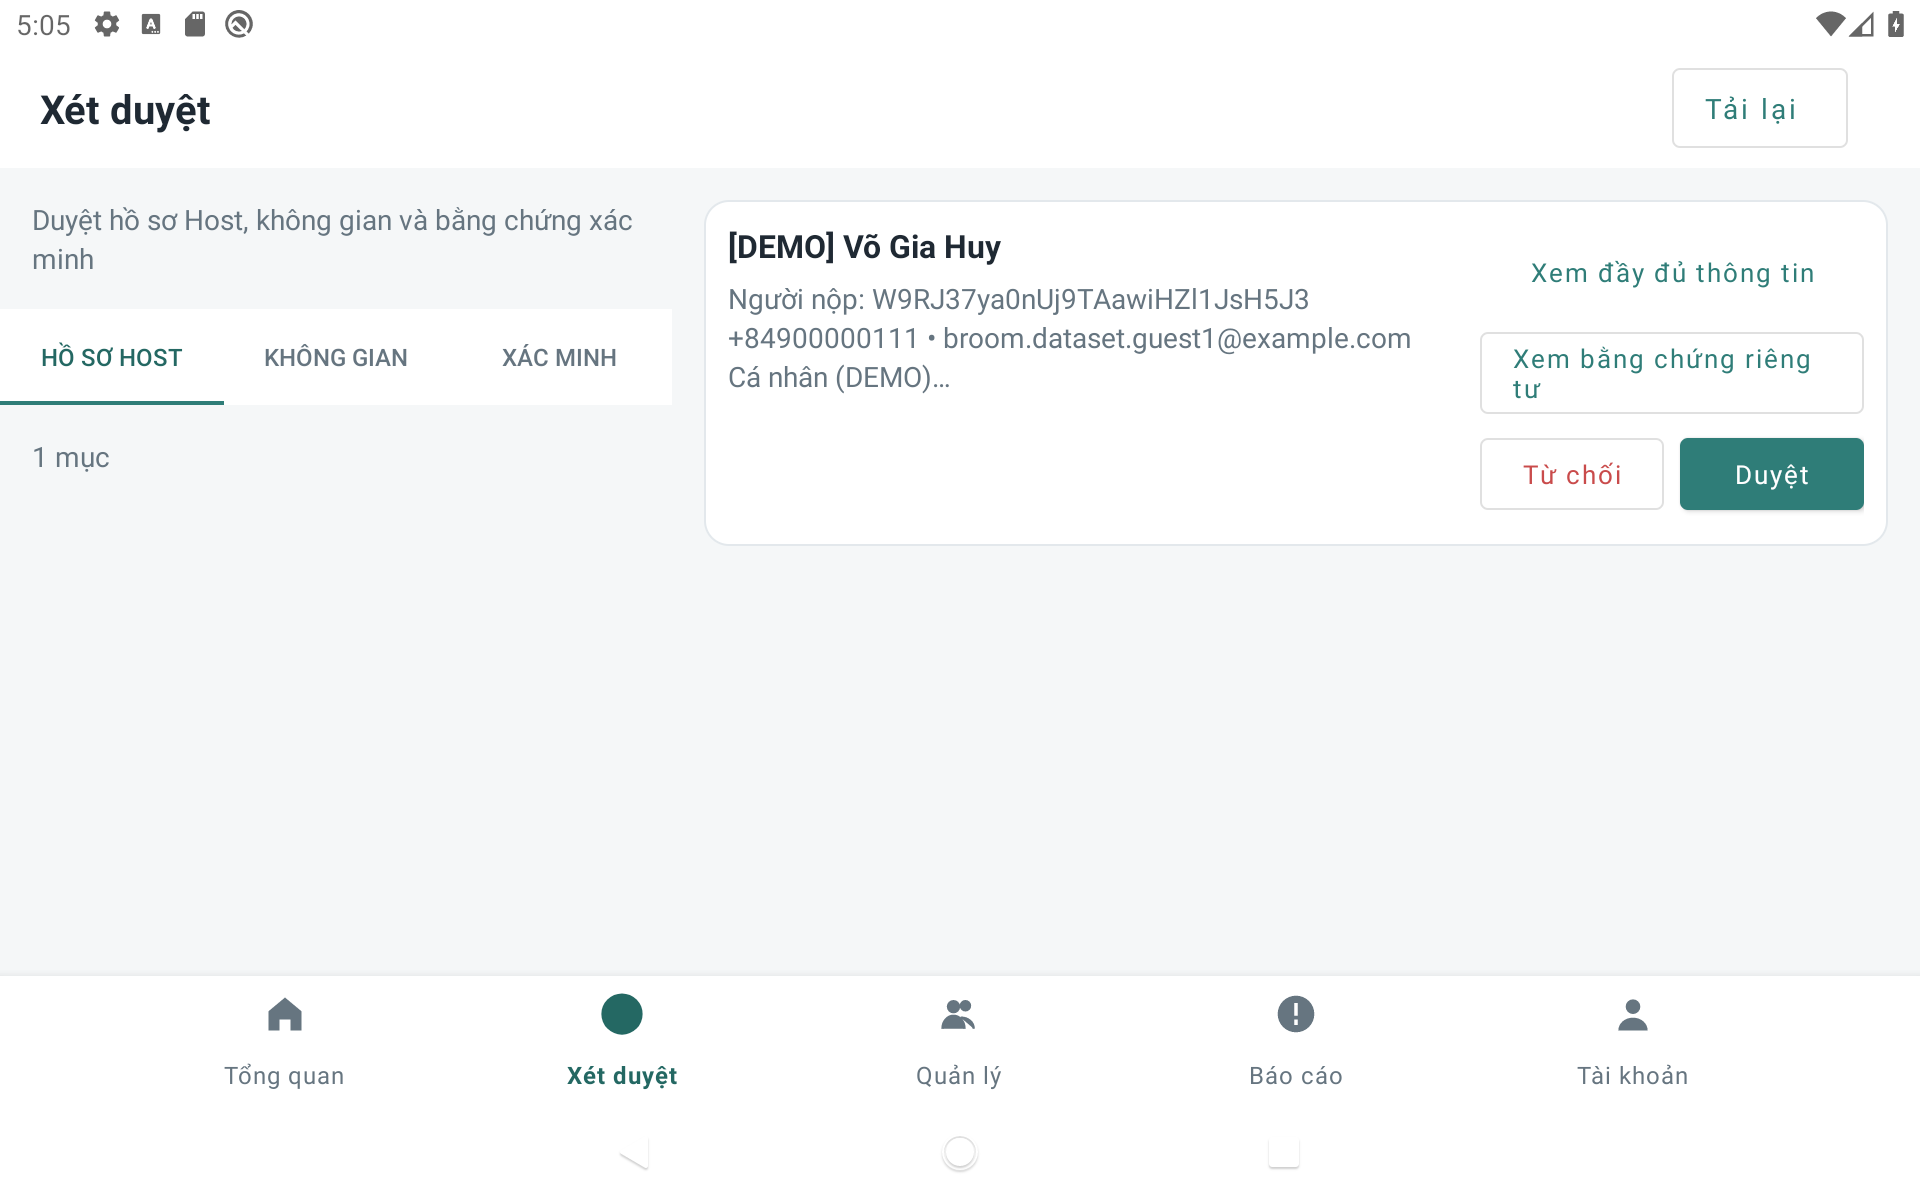
\includegraphics[width=0.94\linewidth]{chapter5/admin-tablet-landscape.png}\\[-1mm]
{\small (b) Tablet ngang}
\caption{Giao diện quản trị theo kích thước thiết bị}
\label{fig:adaptive-admin}
\end{figure}

\clearpage
\subsubsection{Lưu và đọc dữ liệu ngoại tuyến bằng SQLite}
\label{sec:sqlite-offline}
OfflineRepository lưu danh sách, chi tiết phòng và booking của người thuê sau khi tải dữ liệu. OfflineDatabase kế thừa \texttt{SQLiteOpenHelper}, tạo database \texttt{broom\_offline.db} với bảng \texttt{snapshots}. Khóa ghép \texttt{(uid, kind, item\_id)} tách tài khoản, loại bản lưu và đối tượng; \texttt{payload} chứa model đã tuần tự hóa thành dữ liệu nhị phân (BLOB), còn \texttt{saved\_at} ghi thời điểm lưu. Việc đọc, ghi chạy trên luồng nền và trả kết quả về giao diện qua ViewModel \parencite{android_sqlite}.

Hình~\ref{fig:sqlite-offline-screens} thể hiện Trang chủ và lịch sử đặt chỗ khi điện thoại đã ngắt mạng. Danh sách vẫn hiển thị nội dung đã tải, kèm nhãn Ngoại tuyến và thời điểm bản lưu. Người dùng mở được chi tiết phòng hoặc booking; các nút đặt chỗ, thanh toán và cập nhật nghiệp vụ bị khóa. Trang không có bản lưu hiển thị thông báo yêu cầu kết nối mạng để tải dữ liệu.

\begin{figure}[H]\centering
\begin{minipage}[t]{0.32\linewidth}\centering
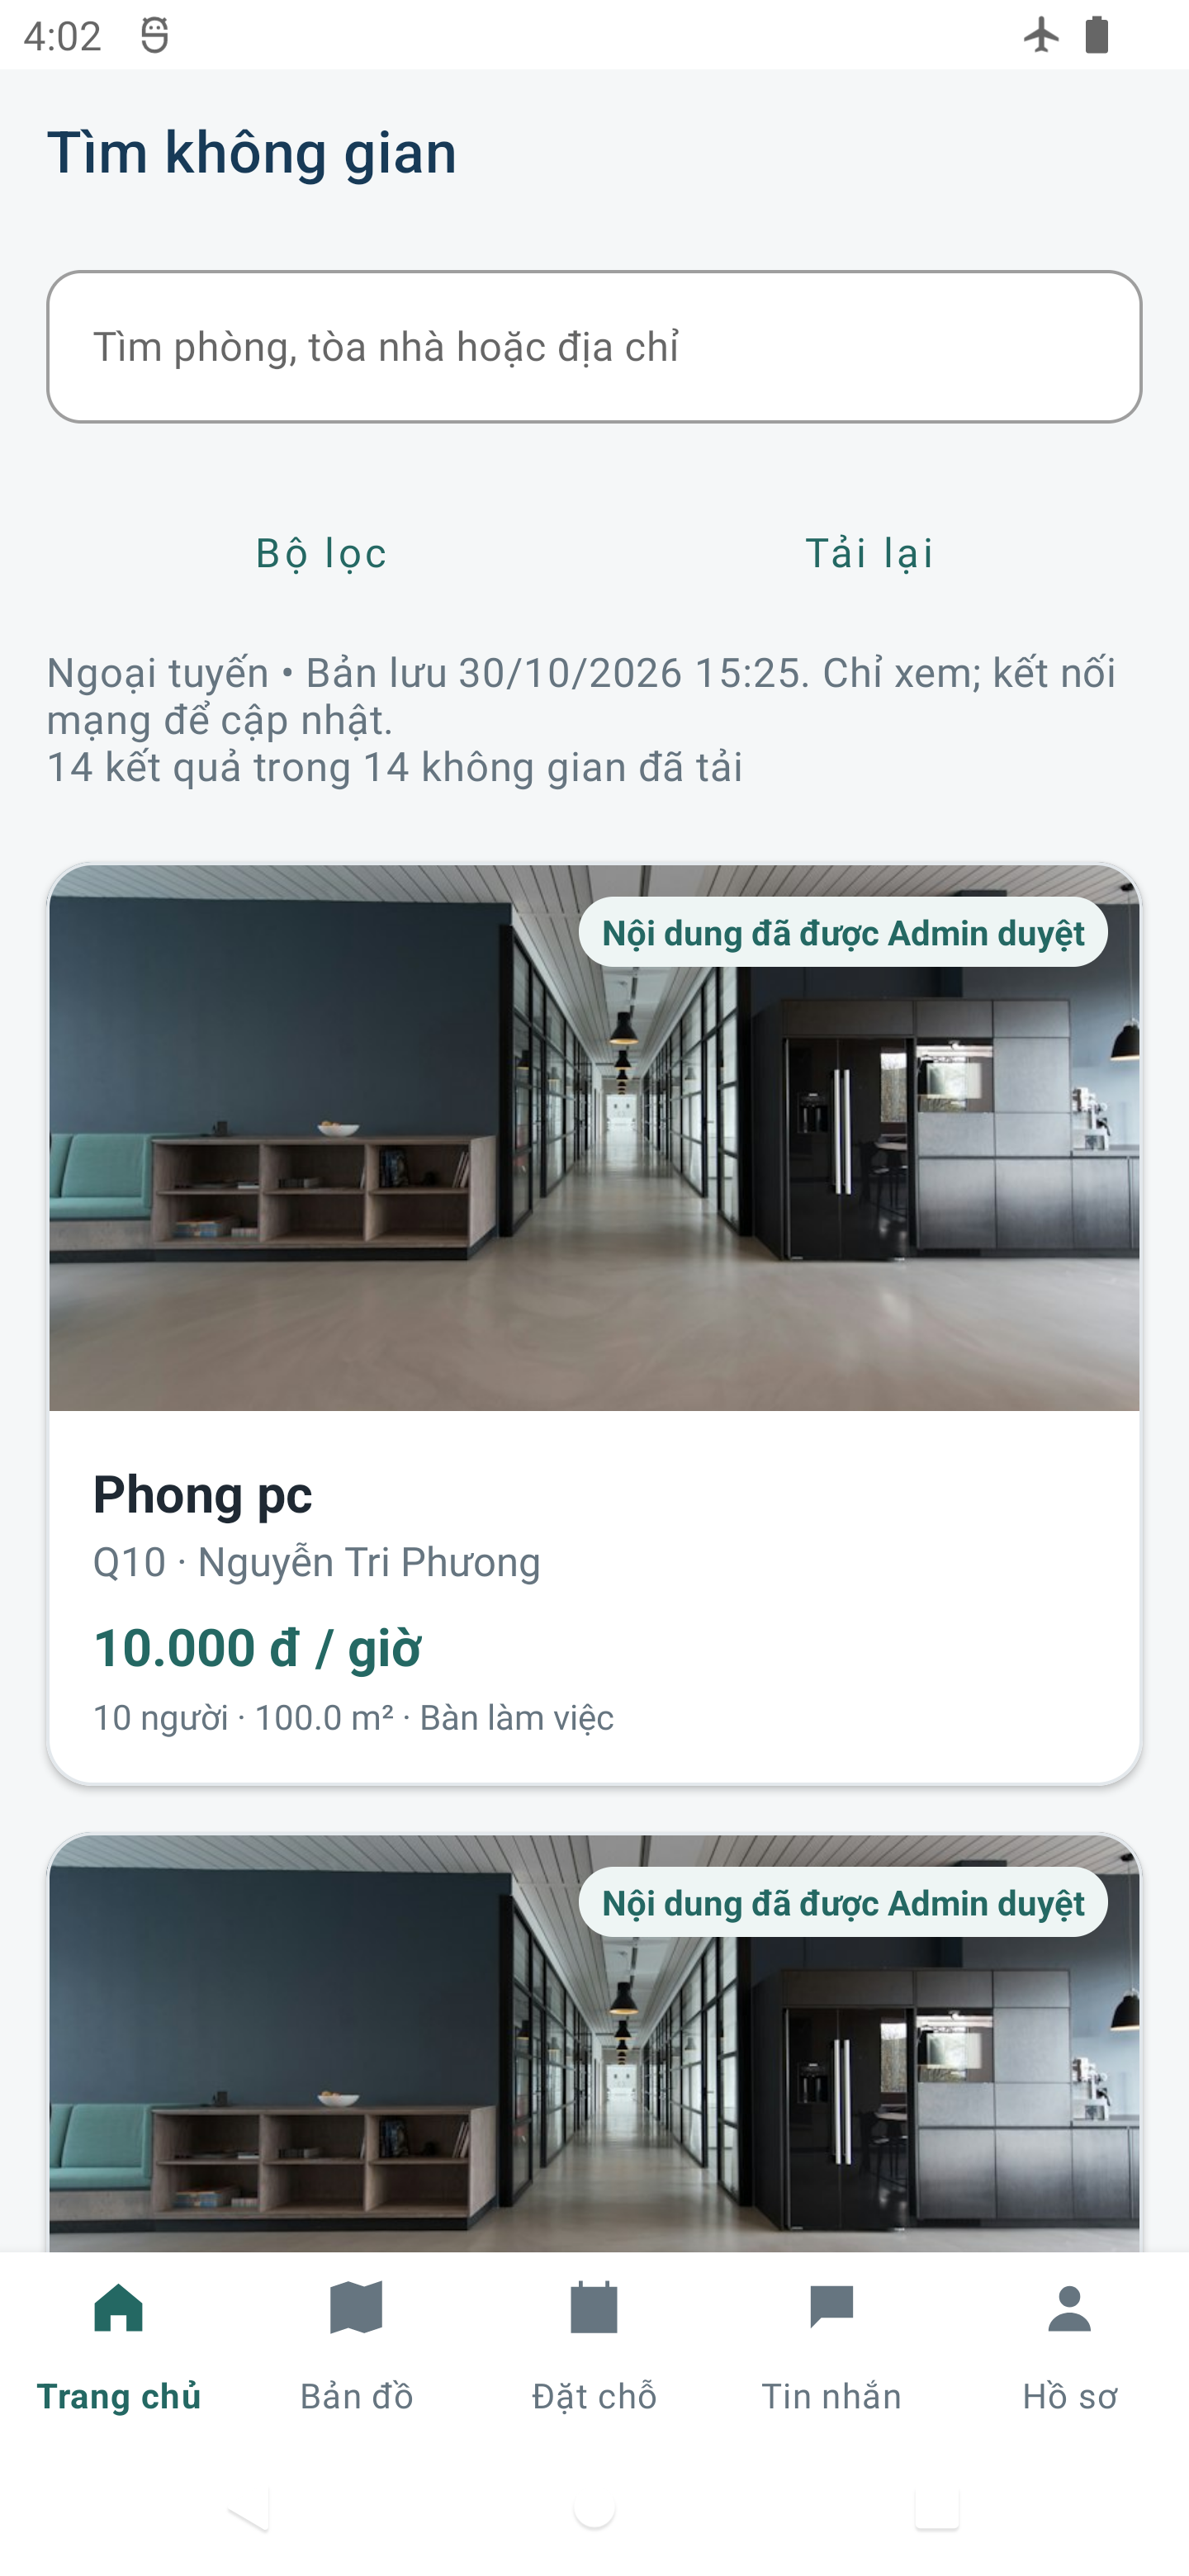
\includegraphics[width=\linewidth]{chapter5/offline/home.png}\\[-1mm]
{\small (a) Phòng đã tải trên Trang chủ}
\end{minipage}\hspace{0.05\linewidth}%
\begin{minipage}[t]{0.32\linewidth}\centering
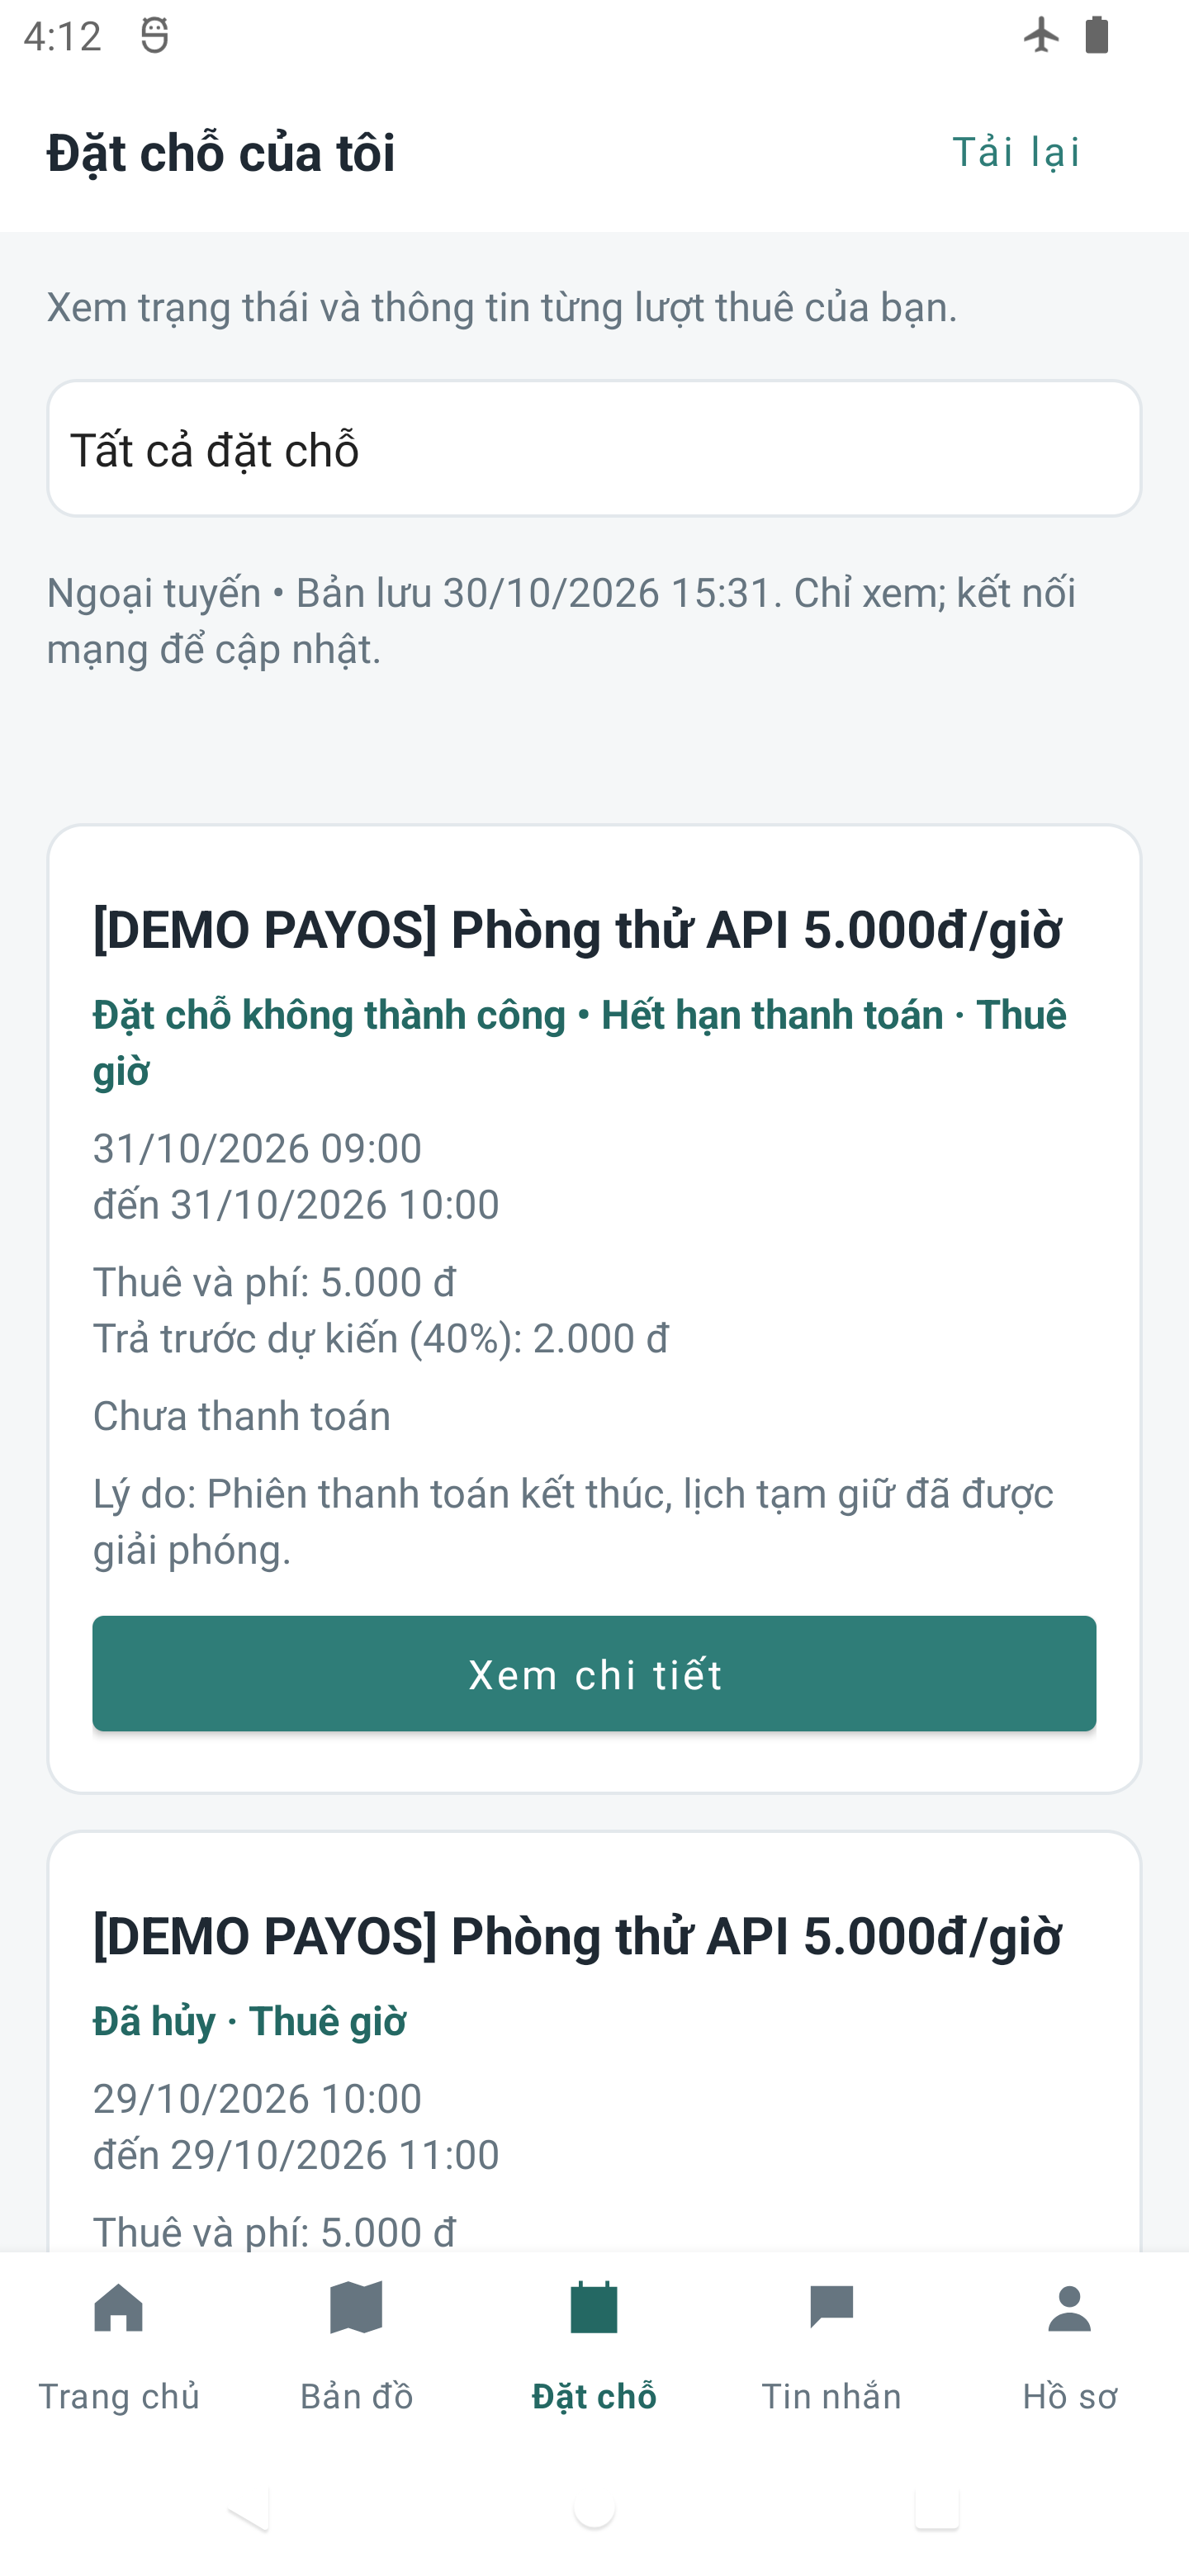
\includegraphics[width=\linewidth]{chapter5/offline/bookings.png}\\[-1mm]
{\small (b) Lịch sử đặt chỗ đã lưu}
\end{minipage}
\caption{Xem dữ liệu từ SQLite khi điện thoại mất kết nối mạng}
\label{fig:sqlite-offline-screens}
\end{figure}

Bản lưu tồn tại sau khi đóng và mở lại ứng dụng. Khi có mạng, SessionActivity kiểm tra phiên và tải dữ liệu hiện tại; lỗi quyền truy cập không được thay bằng kết quả cục bộ. Đăng xuất xóa bản lưu của UID tương ứng. SQLite chỉ lưu dữ liệu để đọc lại, không xếp hàng giao dịch đặt chỗ hoặc thanh toán; ảnh do bộ nhớ đệm của thư viện hiển thị ảnh quản lý riêng.

\endgroup

\chapstart
\section{QUY TRÌNH THỰC THI}
\label{sec:execution-flows}
\begingroup
\setlist[enumerate]{leftmargin=1.27cm,itemsep=3pt,topsep=4pt}
\setlength{\emergencystretch}{1em}
\widowpenalty=10000
\clubpenalty=10000
\subsection{Quy trình đăng ký tài khoản}
Người dùng mở Đăng ký, nhập họ tên, username, email, số điện thoại và mật khẩu như Hình~\ref{fig:registration-reset}(a). Biểu mẫu chỉ gửi khi các trường và xác nhận mật khẩu hợp lệ.

Repository tạo danh tính Authentication rồi ghi \texttt{users/\{uid\}} và alias \texttt{usernames} trong transaction Firestore. Nếu ghi hồ sơ thất bại, hệ thống thử xóa danh tính để bù trừ vì hai dịch vụ không có transaction chung. Thành công thì mở giao diện GUEST.

\subsection{Quy trình đăng nhập và khôi phục mật khẩu}
Người dùng nhập email hoặc username và mật khẩu; username được tra cứu thành email trước khi xác thực. Ứng dụng kiểm tra hồ sơ ACTIVE để mở khu vực người thuê, Host hoặc Admin. Phiên hết hiệu lực, thiếu hồ sơ hoặc bị khóa đều được xử lý trước khi điều hướng.

Khi quên mật khẩu, người dùng nhập email ở Hình~\ref{fig:registration-reset}(b) và đặt lại qua liên kết Firebase. App chỉ thông báo kết quả gửi yêu cầu; người dùng đăng nhập lại sau khi hoàn tất.

\begin{figure}[H]\centering
\begin{minipage}[t]{0.27\linewidth}\centering\vspace{0pt}
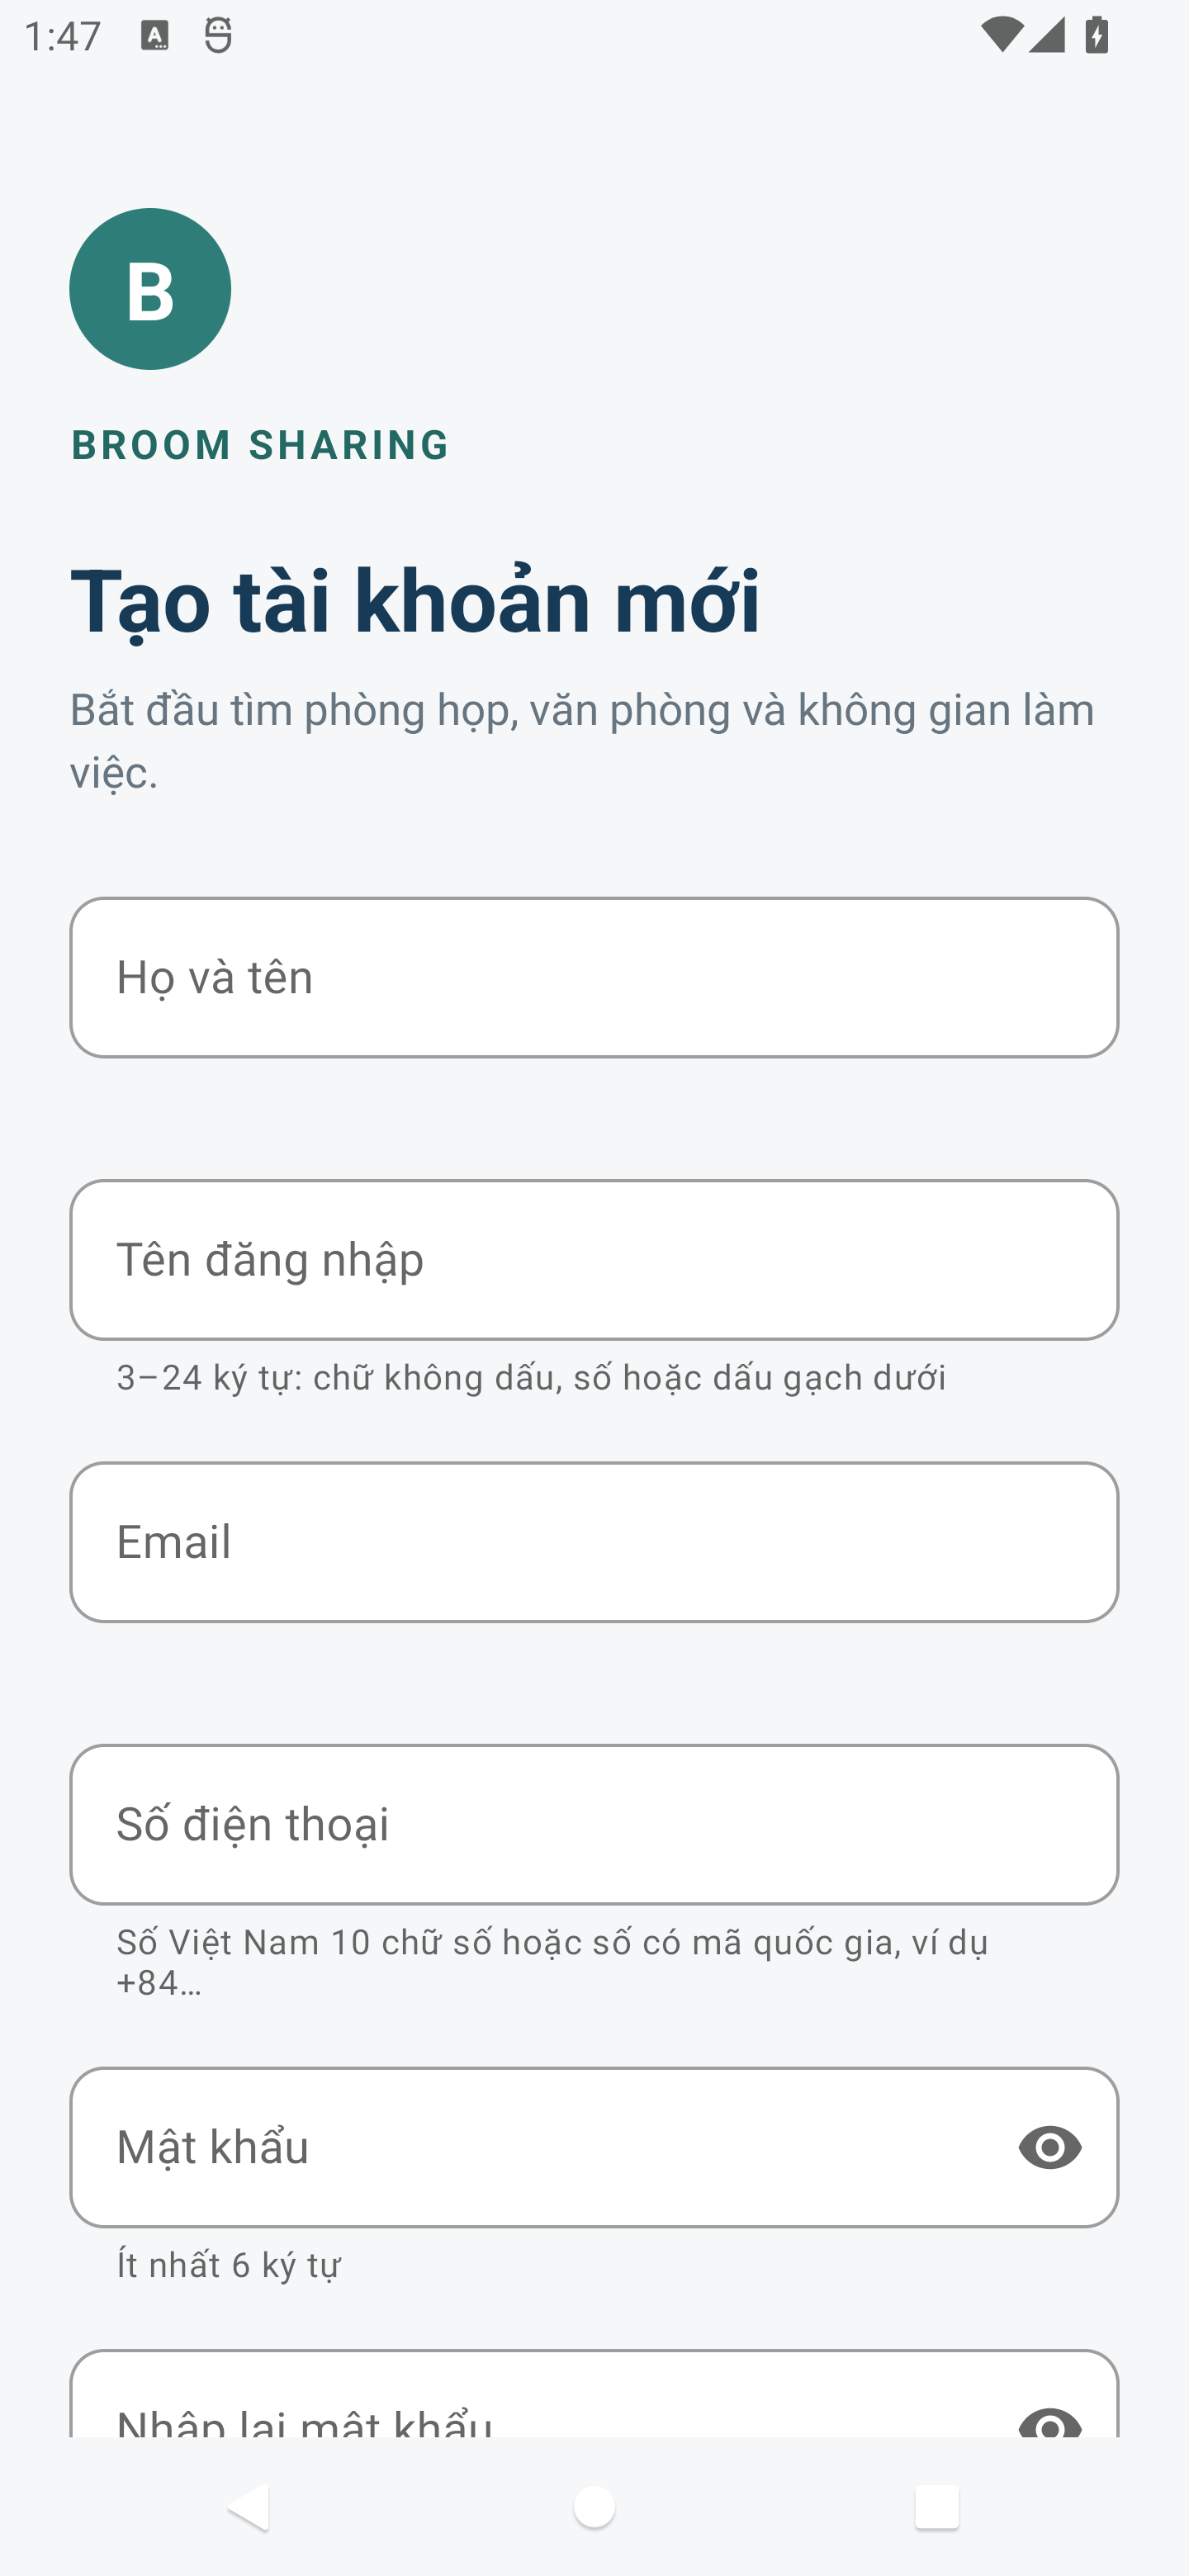
\includegraphics[height=0.35\textheight,width=\linewidth,keepaspectratio]{chapter5/final/register.png}\\[-1mm]
{\small (a) Nhập hồ sơ đăng ký}
\end{minipage}\hspace{0.05\linewidth}%
\begin{minipage}[t]{0.27\linewidth}\centering\vspace{0pt}
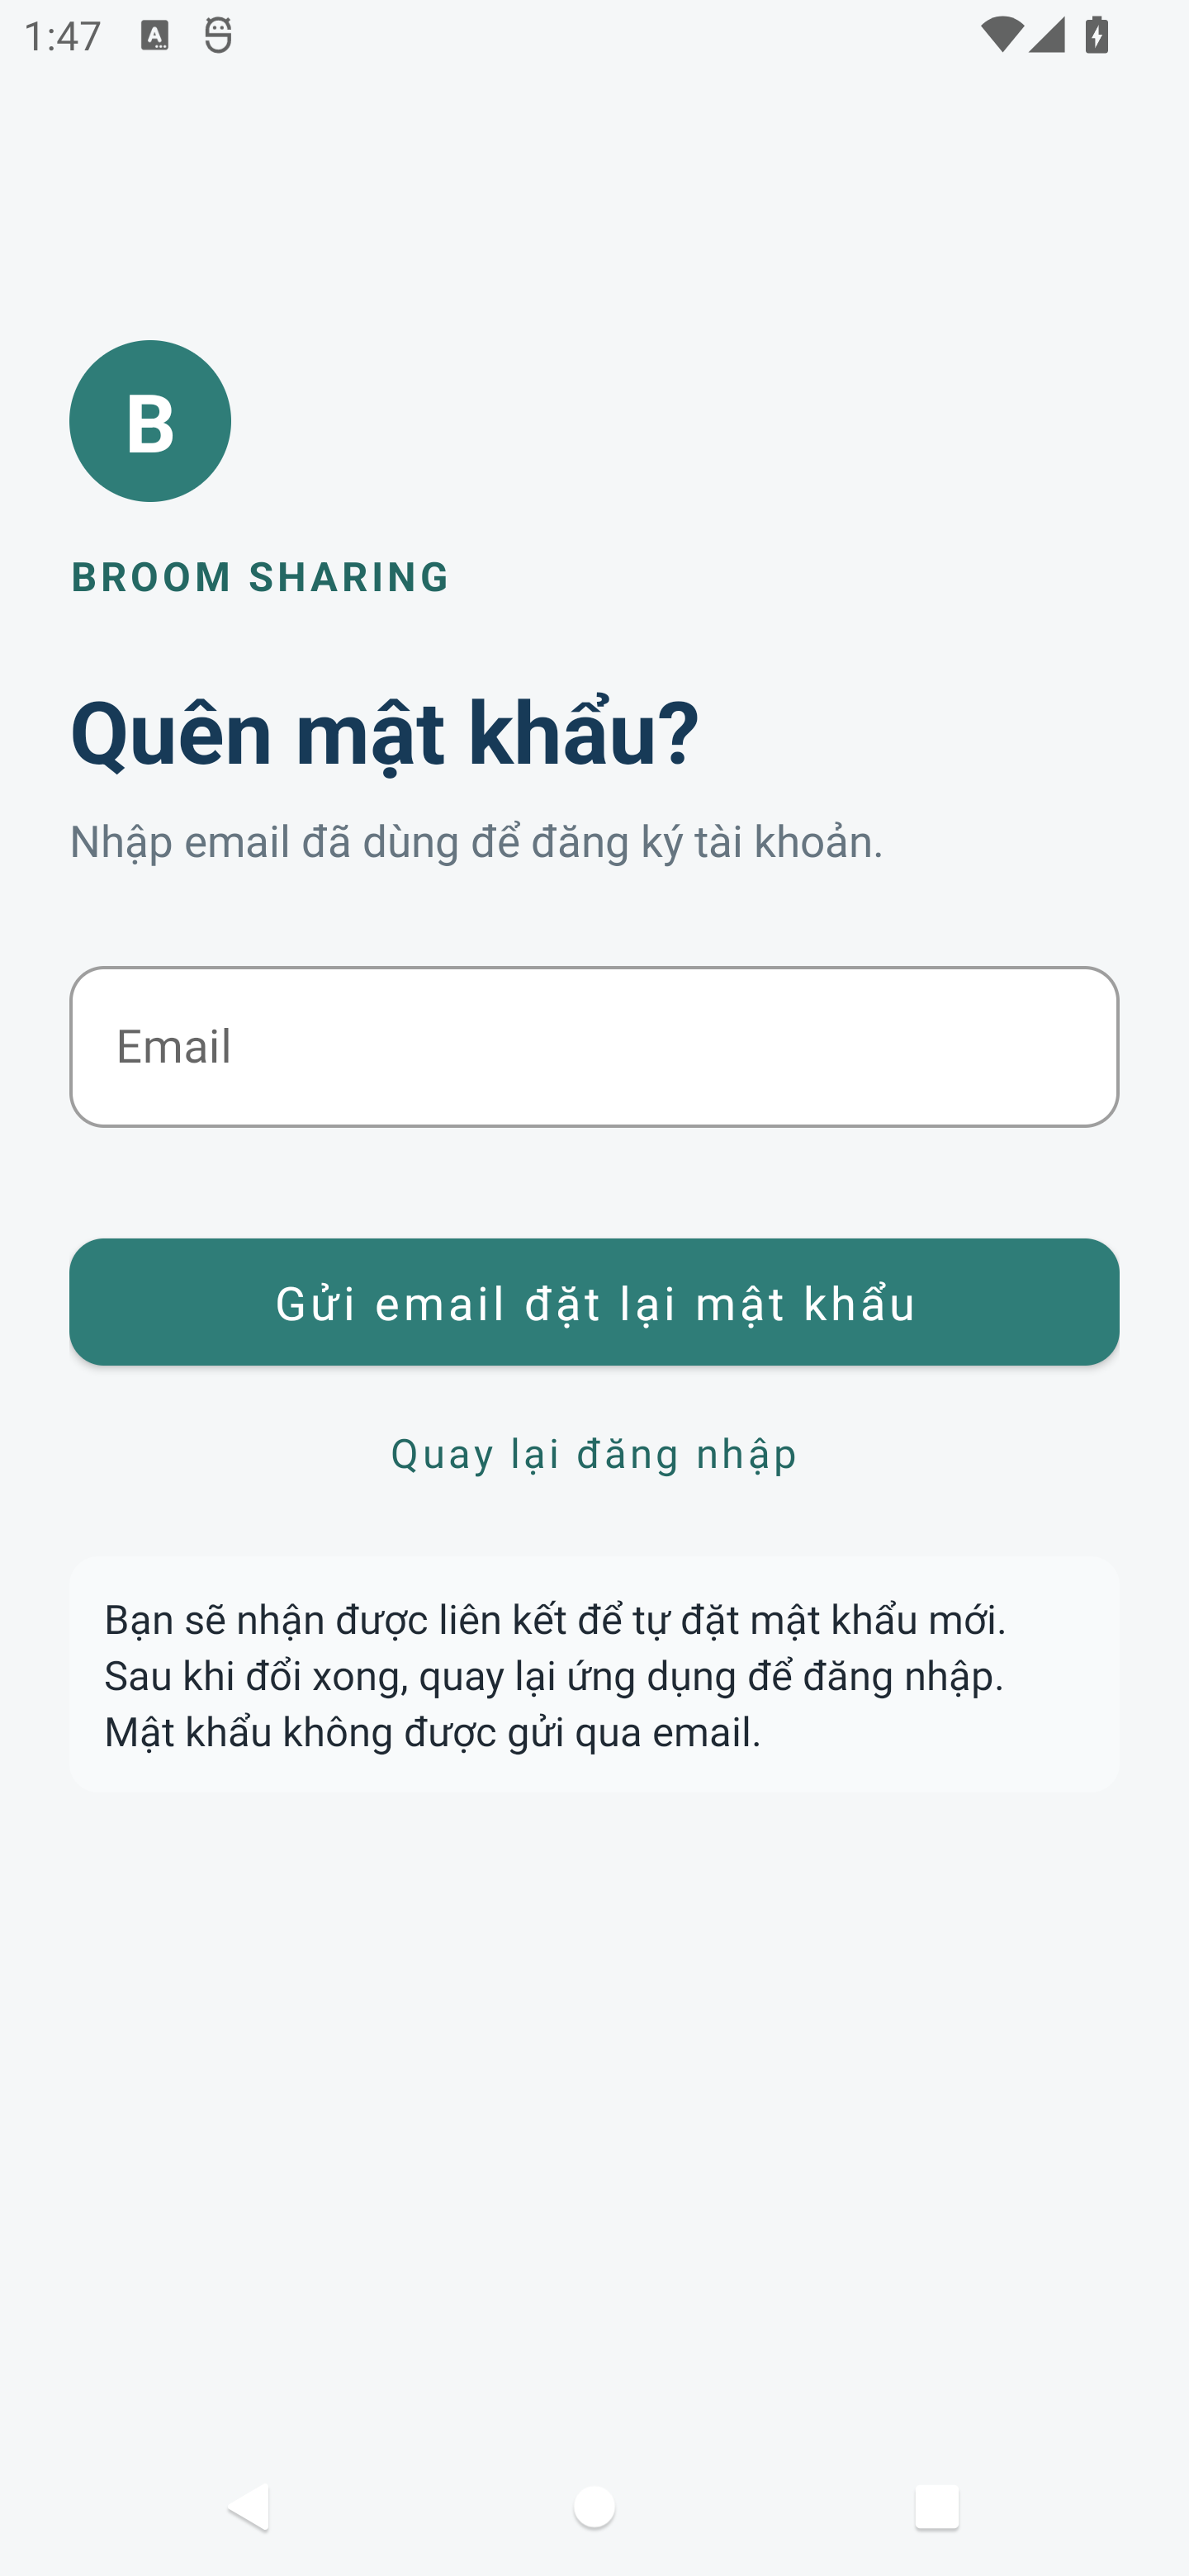
\includegraphics[height=0.35\textheight,width=\linewidth,keepaspectratio]{chapter5/final/reset-password.png}\\[-1mm]
{\small (b) Gửi yêu cầu đặt lại mật khẩu}
\end{minipage}
\caption{Các biểu mẫu đăng ký và khôi phục mật khẩu hiện thực}
\label{fig:registration-reset}
\end{figure}

\subsection{Quy trình đăng ký Host và công bố không gian}
\subsubsection{Nộp hồ sơ và xét duyệt quyền Host}
Tài khoản GUEST đang hoạt động mở đơn xin quyền Host, khai báo thông tin liên hệ, loại tổ chức và hai ảnh giấy tờ DEMO. Ứng dụng kiểm tra tệp, tải ảnh và gửi URL cùng hồ sơ; kết quả nộp thành công là đơn PENDING, chưa có quyền đăng phòng. Dữ liệu giấy tờ dùng trong đồ án không chứng minh danh tính pháp lý ngoài thực tế.

Admin mở hàng đợi hồ sơ trong Hình~\ref{fig:admin-application-evidence}(a), xem nội dung và ảnh trước khi quyết định. Chấp thuận cập nhật đồng thời đơn APPROVED, quyền HOST, bản chiếu PublicHost và audit. Từ chối lưu lý do để người nộp bổ sung và gửi lại theo điều kiện của đơn.

Hình~\ref{fig:host-role-transition} ghi nhận cùng một tài khoản DEMO trước và sau khi được cấp quyền. Ban đầu, hồ sơ hiển thị vai trò người thuê và lối vào đăng ký Host; sau xét duyệt, tài khoản mở được kênh người cho thuê. Quyền mới bổ sung khả năng quản lý không gian, đồng thời vẫn cho phép chuyển sang giao diện thuê.

\begin{figure}[H]\centering
\begin{minipage}[t]{0.34\linewidth}\centering
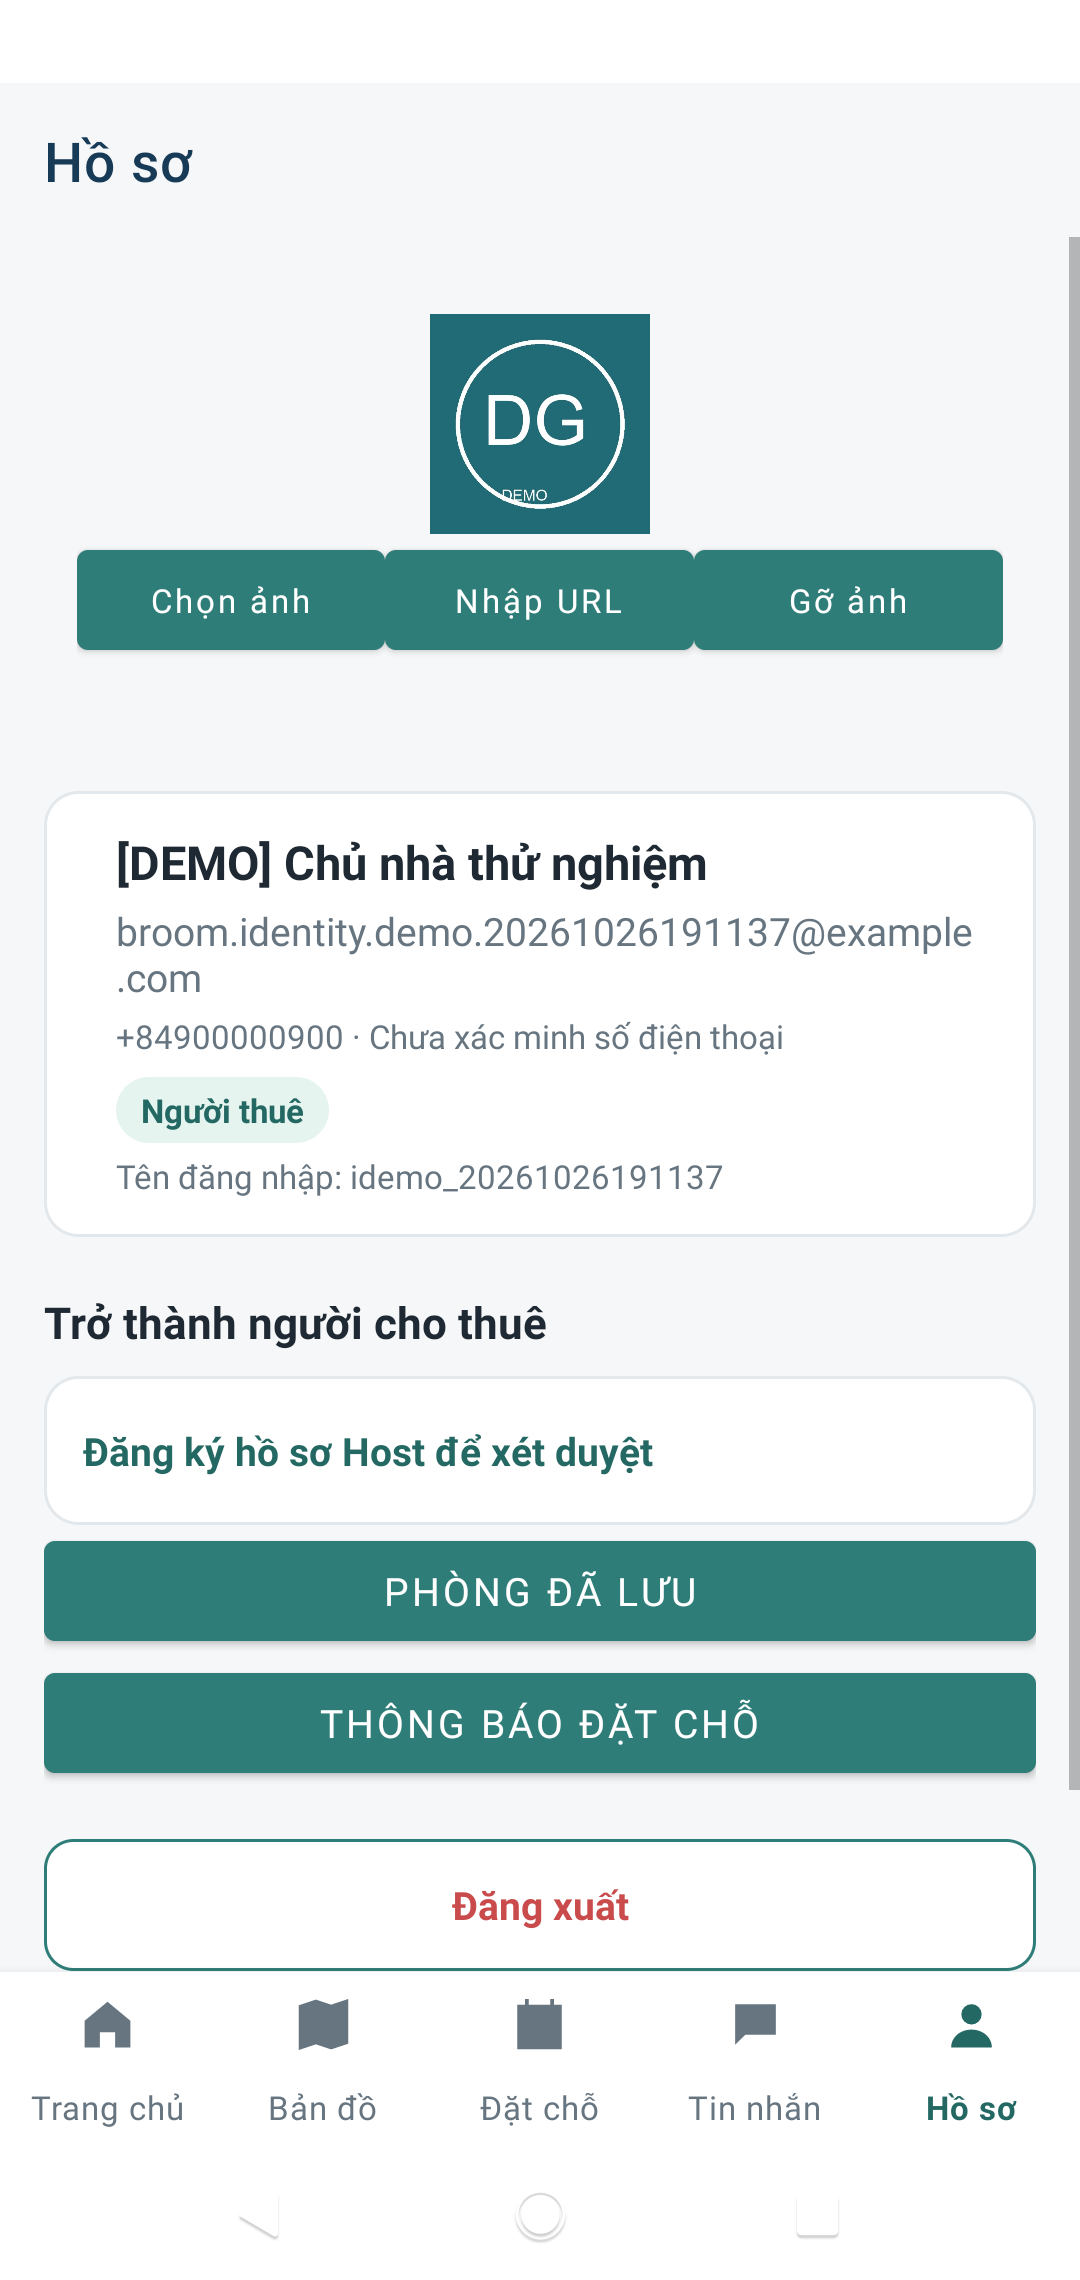
\includegraphics[width=\linewidth]{chapter6/host-role-before.png}\\[-1mm]
{\small (a) Trước khi được cấp quyền}
\end{minipage}\hspace{0.05\linewidth}%
\begin{minipage}[t]{0.34\linewidth}\centering
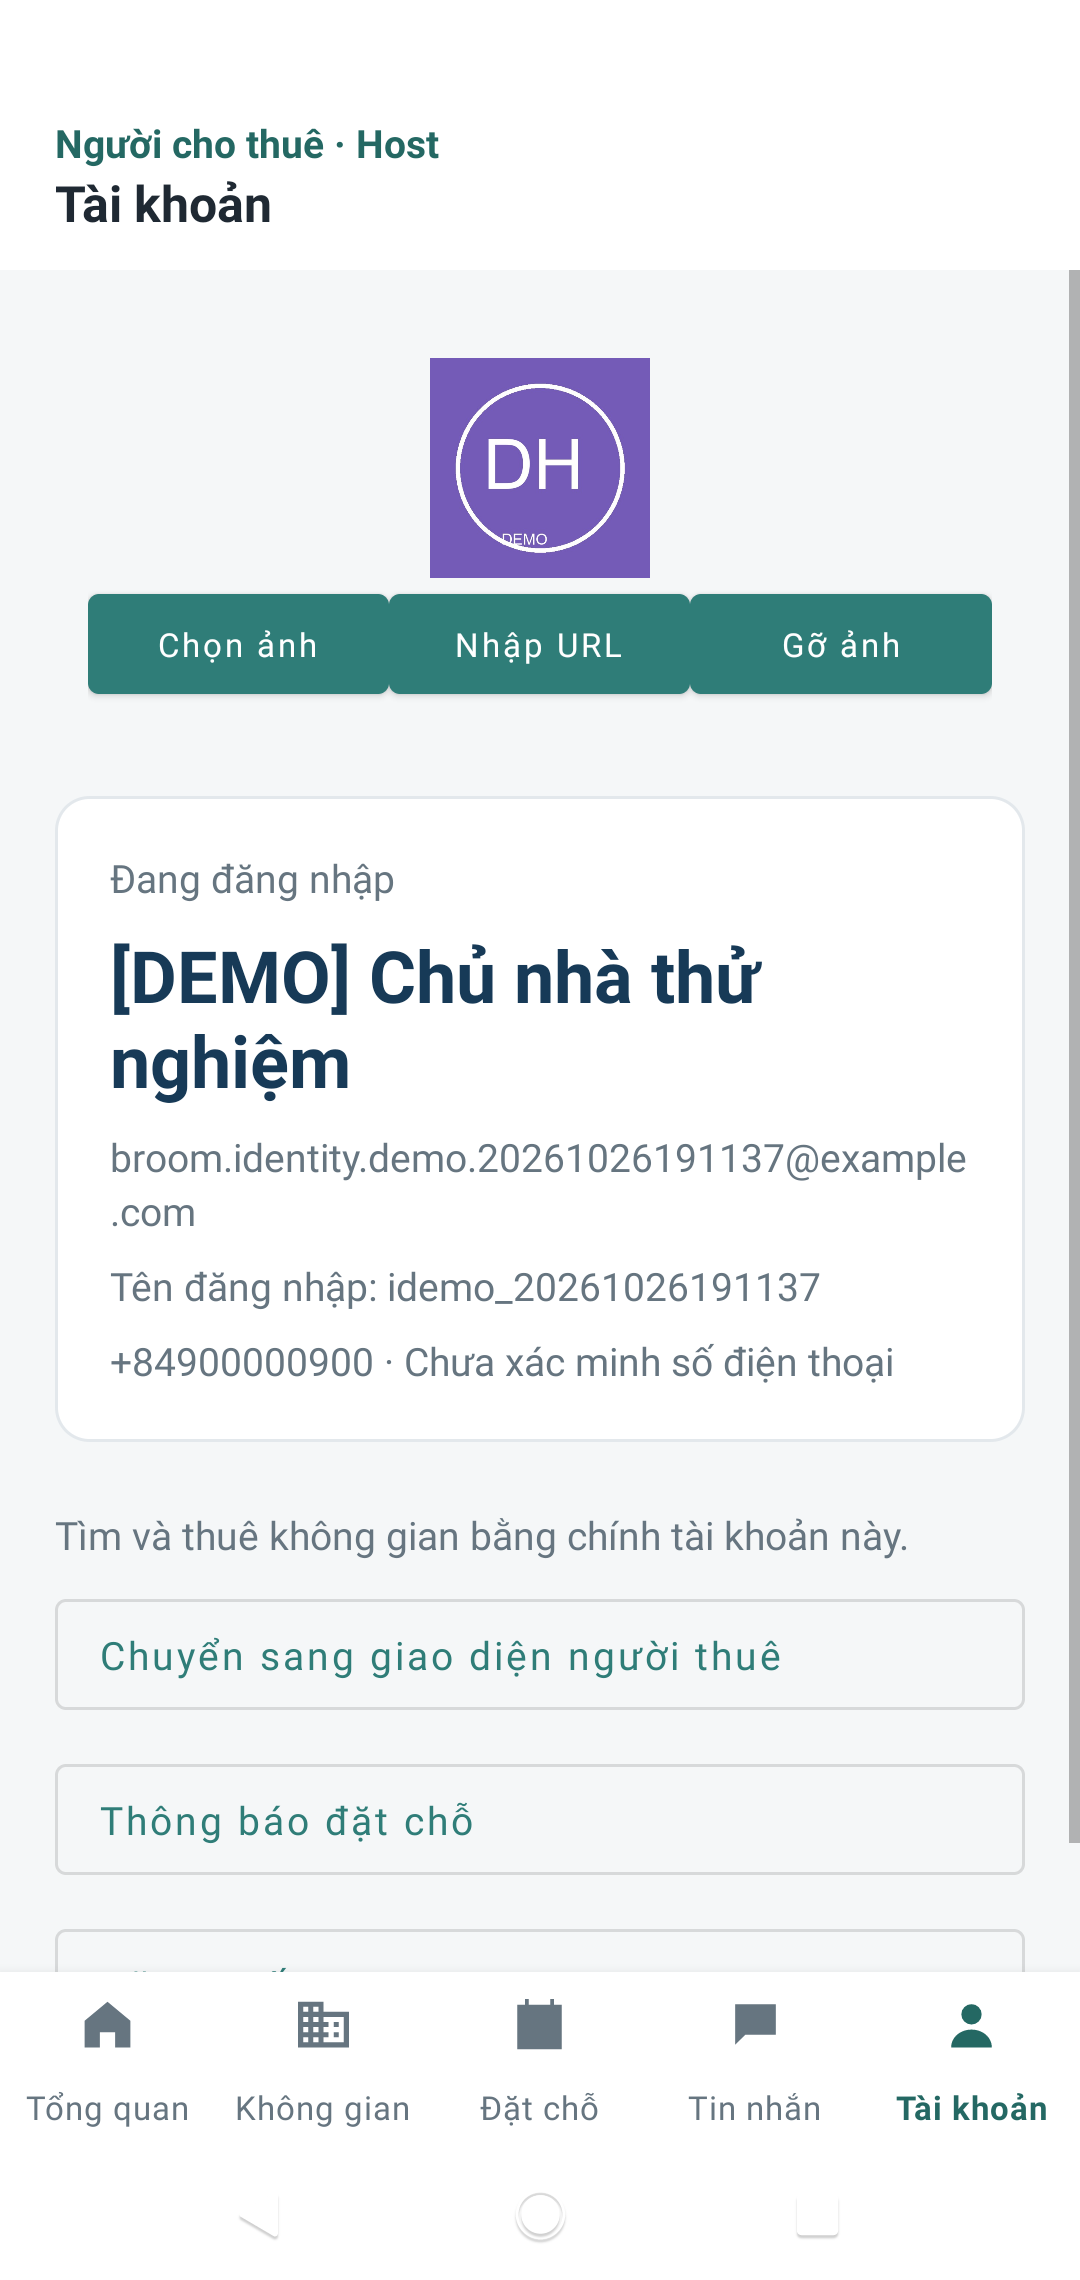
\includegraphics[width=\linewidth]{chapter6/host-role-after.png}\\[-1mm]
{\small (b) Tài khoản đã có quyền Host}
\end{minipage}
\caption{Thay đổi quyền của tài khoản sau quy trình xét duyệt Host}
\label{fig:host-role-transition}
\end{figure}

\Needspace{9\baselineskip}
\subsubsection{Tạo, xét duyệt và công bố không gian}
Sau khi được cấp quyền, Host thực hiện trình tự sau:
\begin{enumerate}
\item Tạo tòa nhà với địa chỉ, liên hệ và vị trí; sau đó mở biểu mẫu phòng, chọn tòa nhà thuộc sở hữu và nhập thông tin cơ bản, ảnh, tiện ích.
\item Chọn thuê giờ hoặc tháng/quý, thiết lập giá và lịch phù hợp. Kiểm tra ngày làm việc, khung giờ, thời lượng tối thiểu hoặc tháng bắt đầu thuê cố định; lưu nháp nếu chưa hoàn tất.
\item Gửi bài đăng xét duyệt. Admin đọc thông tin phòng và đối tượng liên quan, chấp thuận hoặc từ chối kèm lý do. Host theo dõi kết quả và mở cho thuê khi đáp ứng điều kiện.
\end{enumerate}

Phòng chỉ xuất hiện với người thuê khi APPROVED và ACTIVE. Duyệt đơn Host không tự duyệt phòng; xét duyệt minh chứng vị trí/ảnh cũng là hồ sơ riêng. Khi sửa cấu hình có ảnh hưởng lịch, hệ thống kiểm tra các booking đang giữ chỗ để bảo toàn kỳ thuê đã đặt. Hình~\ref{fig:actual-host-editor} minh họa dữ liệu đầu vào, còn Hình~\ref{fig:admin-overview-review} thể hiện bước xét duyệt tin đăng.

Hình~\ref{fig:room-publication-stages} minh họa cách Host theo dõi kết quả công bố theo từng phòng. Nhãn đã duyệt và đang hiển thị được đặt trên thẻ phòng; các nút chỉnh sửa và lịch đặt mở thao tác tương ứng. Màn Admin tại Hình~\ref{fig:admin-overview-review}(b) thực hiện bước xét duyệt riêng; việc duyệt tin đăng độc lập với xác nhận booking sau thanh toán.

\begin{figure}[H]\centering
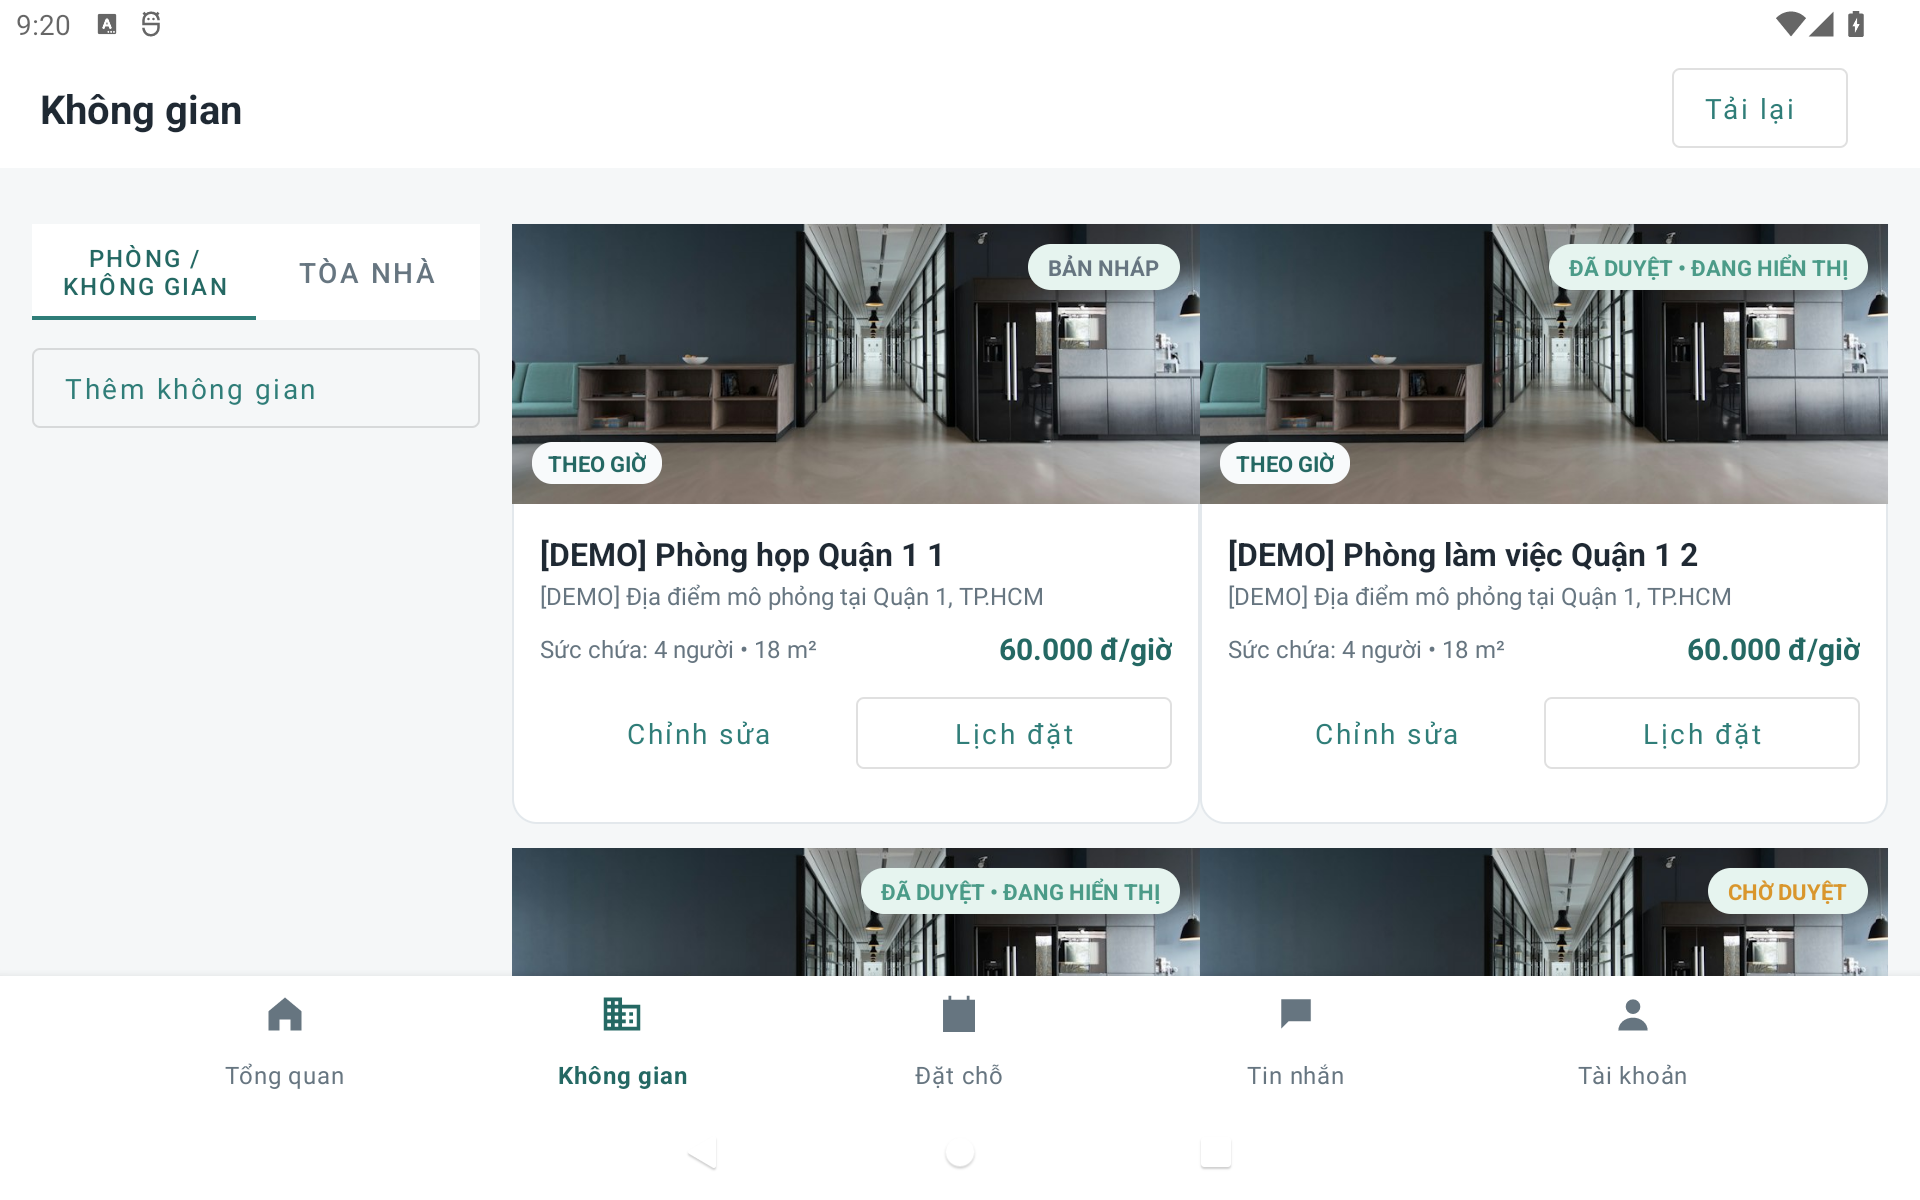
\includegraphics[width=0.96\linewidth]{chapter5/members/host-tablet-spaces-landscape.png}
\caption{Host theo dõi trạng thái công bố và thao tác trên từng phòng}
\label{fig:room-publication-stages}
\end{figure}

\Needspace{10\baselineskip}
\subsection{Quy trình đặt chỗ và thanh toán}
\label{sec:execution-booking-payment}

Quy trình bắt đầu khi người thuê đã đăng nhập và lựa chọn một không gian đang được công bố. Phòng có một hình thức thuê đang hoạt động: theo giờ hoặc theo tháng/quý. Người thuê chọn thời gian theo hình thức đó, không tự chuyển loại thuê của phòng. Trong phiên bản hiện tại, bước thanh toán QR được áp dụng cho phòng thuộc Host demo đã cấu hình kênh payOS.

\Needspace{7\baselineskip}
\subsubsection{Lựa chọn không gian và kiểm tra thời gian thuê}
Người thuê thực hiện các bước sau trước khi mở phiên thanh toán:
\begin{enumerate}
\item Từ danh sách hoặc bản đồ, mở chi tiết phòng để xem ảnh, địa chỉ, tiện ích, giá và điều kiện sử dụng, sau đó chọn đặt chỗ.
\item Chọn ngày và khung giờ nếu thuê theo giờ; chọn kỳ một hoặc ba tháng nếu thuê cố định. Màn hình đọc lịch để thể hiện khoảng đã thuê hoặc đang giữ tạm.
\item Thực hiện kiểm tra lịch và giá. Hệ thống đối chiếu lịch hoạt động, khoảng khóa và các booking đang giữ chỗ, rồi hiển thị tiền thuê cùng khoản trả trước 40\% như Hình~\ref{fig:booking-quote-qr}.
\end{enumerate}

Kết quả kiểm tra không thay cho việc giữ lịch. Khi người thuê nhấn thanh toán, transaction đọc lại dữ liệu và tạo booking PENDING cùng phần giữ lịch tạm. Yêu cầu vừa bị người khác đặt trùng phải được kiểm tra lại; việc gửi lại cùng yêu cầu không được tạo thêm một lượt thuê độc lập. Booking lưu giá và thời gian đã chốt để tiếp tục bước thanh toán.

\subsubsection{Thanh toán QR và xác nhận đặt chỗ}
Sau khi tạo booking, ứng dụng gọi backend Java để lấy giao dịch payOS và chuyển thẳng tới màn QR. Backend xác minh ID token, người thuê của booking và Host thuộc kênh demo; số tiền được lấy từ snapshot, không nhận giá do client tự khai báo. Hạn phiên là mốc đến trước giữa thời điểm tạo booking cộng năm phút và giờ bắt đầu thuê. Việc mở lại QR không làm tính lại thời hạn từ đầu.

\IfFileExists{Resources/chapter6/booking-qr.png}{%
\begin{figure}[H]
\begin{minipage}{\linewidth}
\setlength{\parindent}{1.27cm}
\setstretch{1.4}
Trong Hình~\ref{fig:booking-quote-qr}(a), lượt thuê một giờ có giá 5.000 đồng và khoản trả trước 2.000 đồng. Sau khi gửi yêu cầu, màn QR ở Hình~\ref{fig:booking-quote-qr}(b) hiển thị đúng khoản tiền này, mã giao dịch, người nhận và thời gian còn lại. Người thuê chuyển khoản theo QR hoặc mở trang payOS. Nếu rời màn hình, thẻ tiếp tục thanh toán và thông báo điện thoại dẫn về đúng giao dịch còn hạn; thời gian giữ lịch không bắt đầu lại.
\par\medskip
\centering
\begin{minipage}[t]{0.40\linewidth}\centering
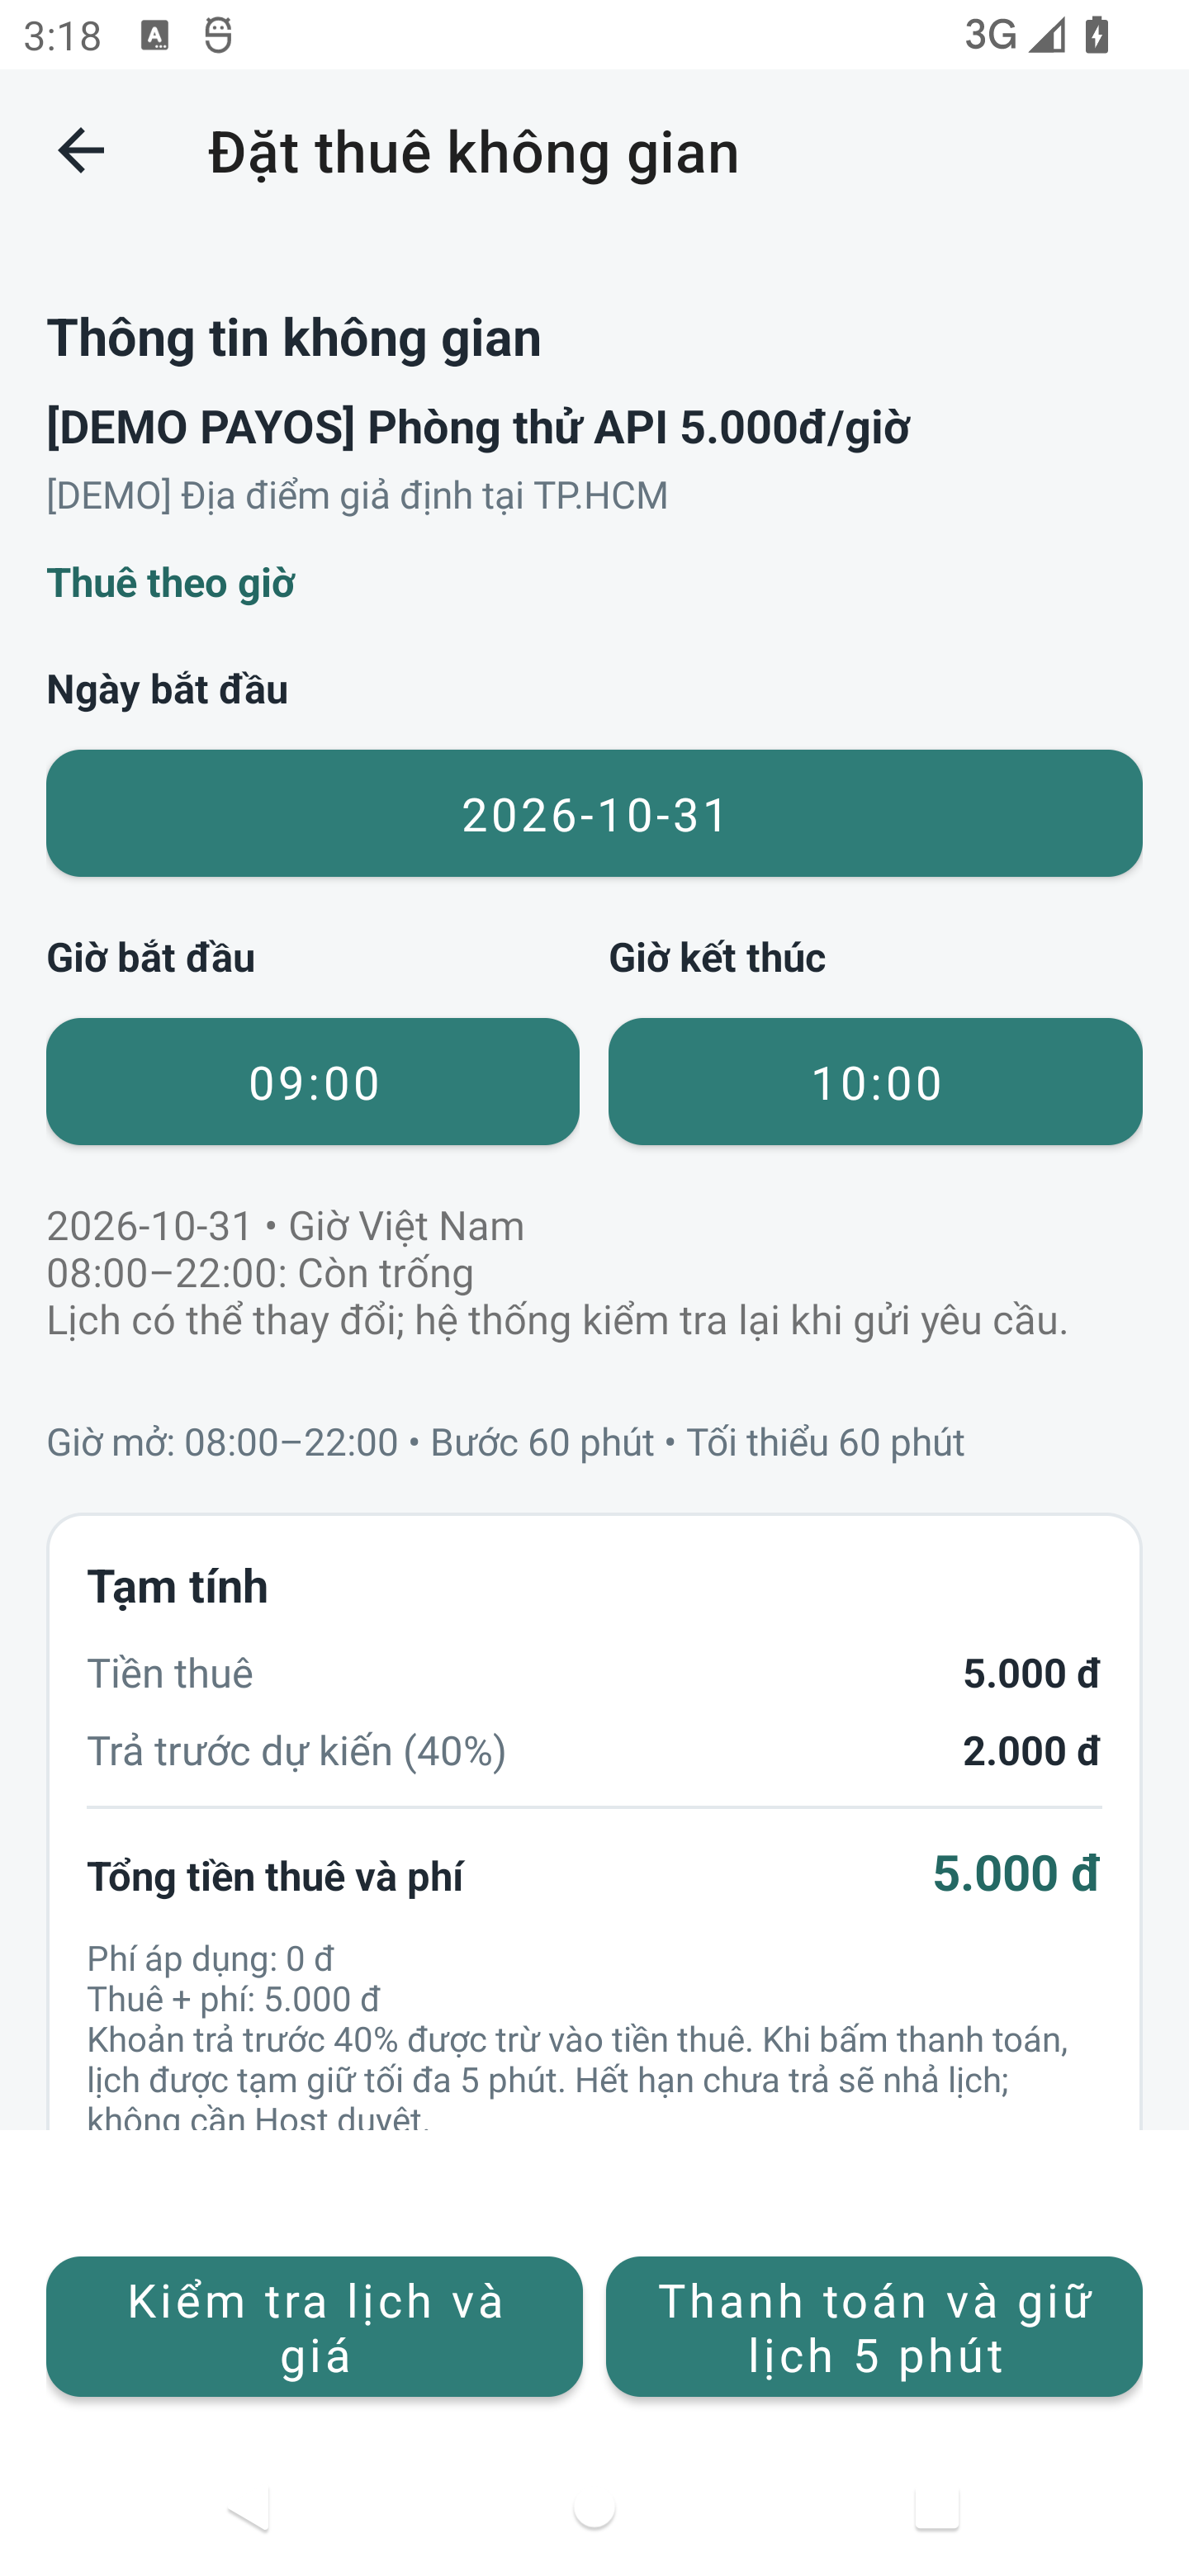
\includegraphics[width=\linewidth]{chapter6/booking-quote.png}\\[-1mm]
{\small (a) Kết quả kiểm tra lịch và giá}
\end{minipage}\hspace{0.05\linewidth}%
\begin{minipage}[t]{0.40\linewidth}\centering
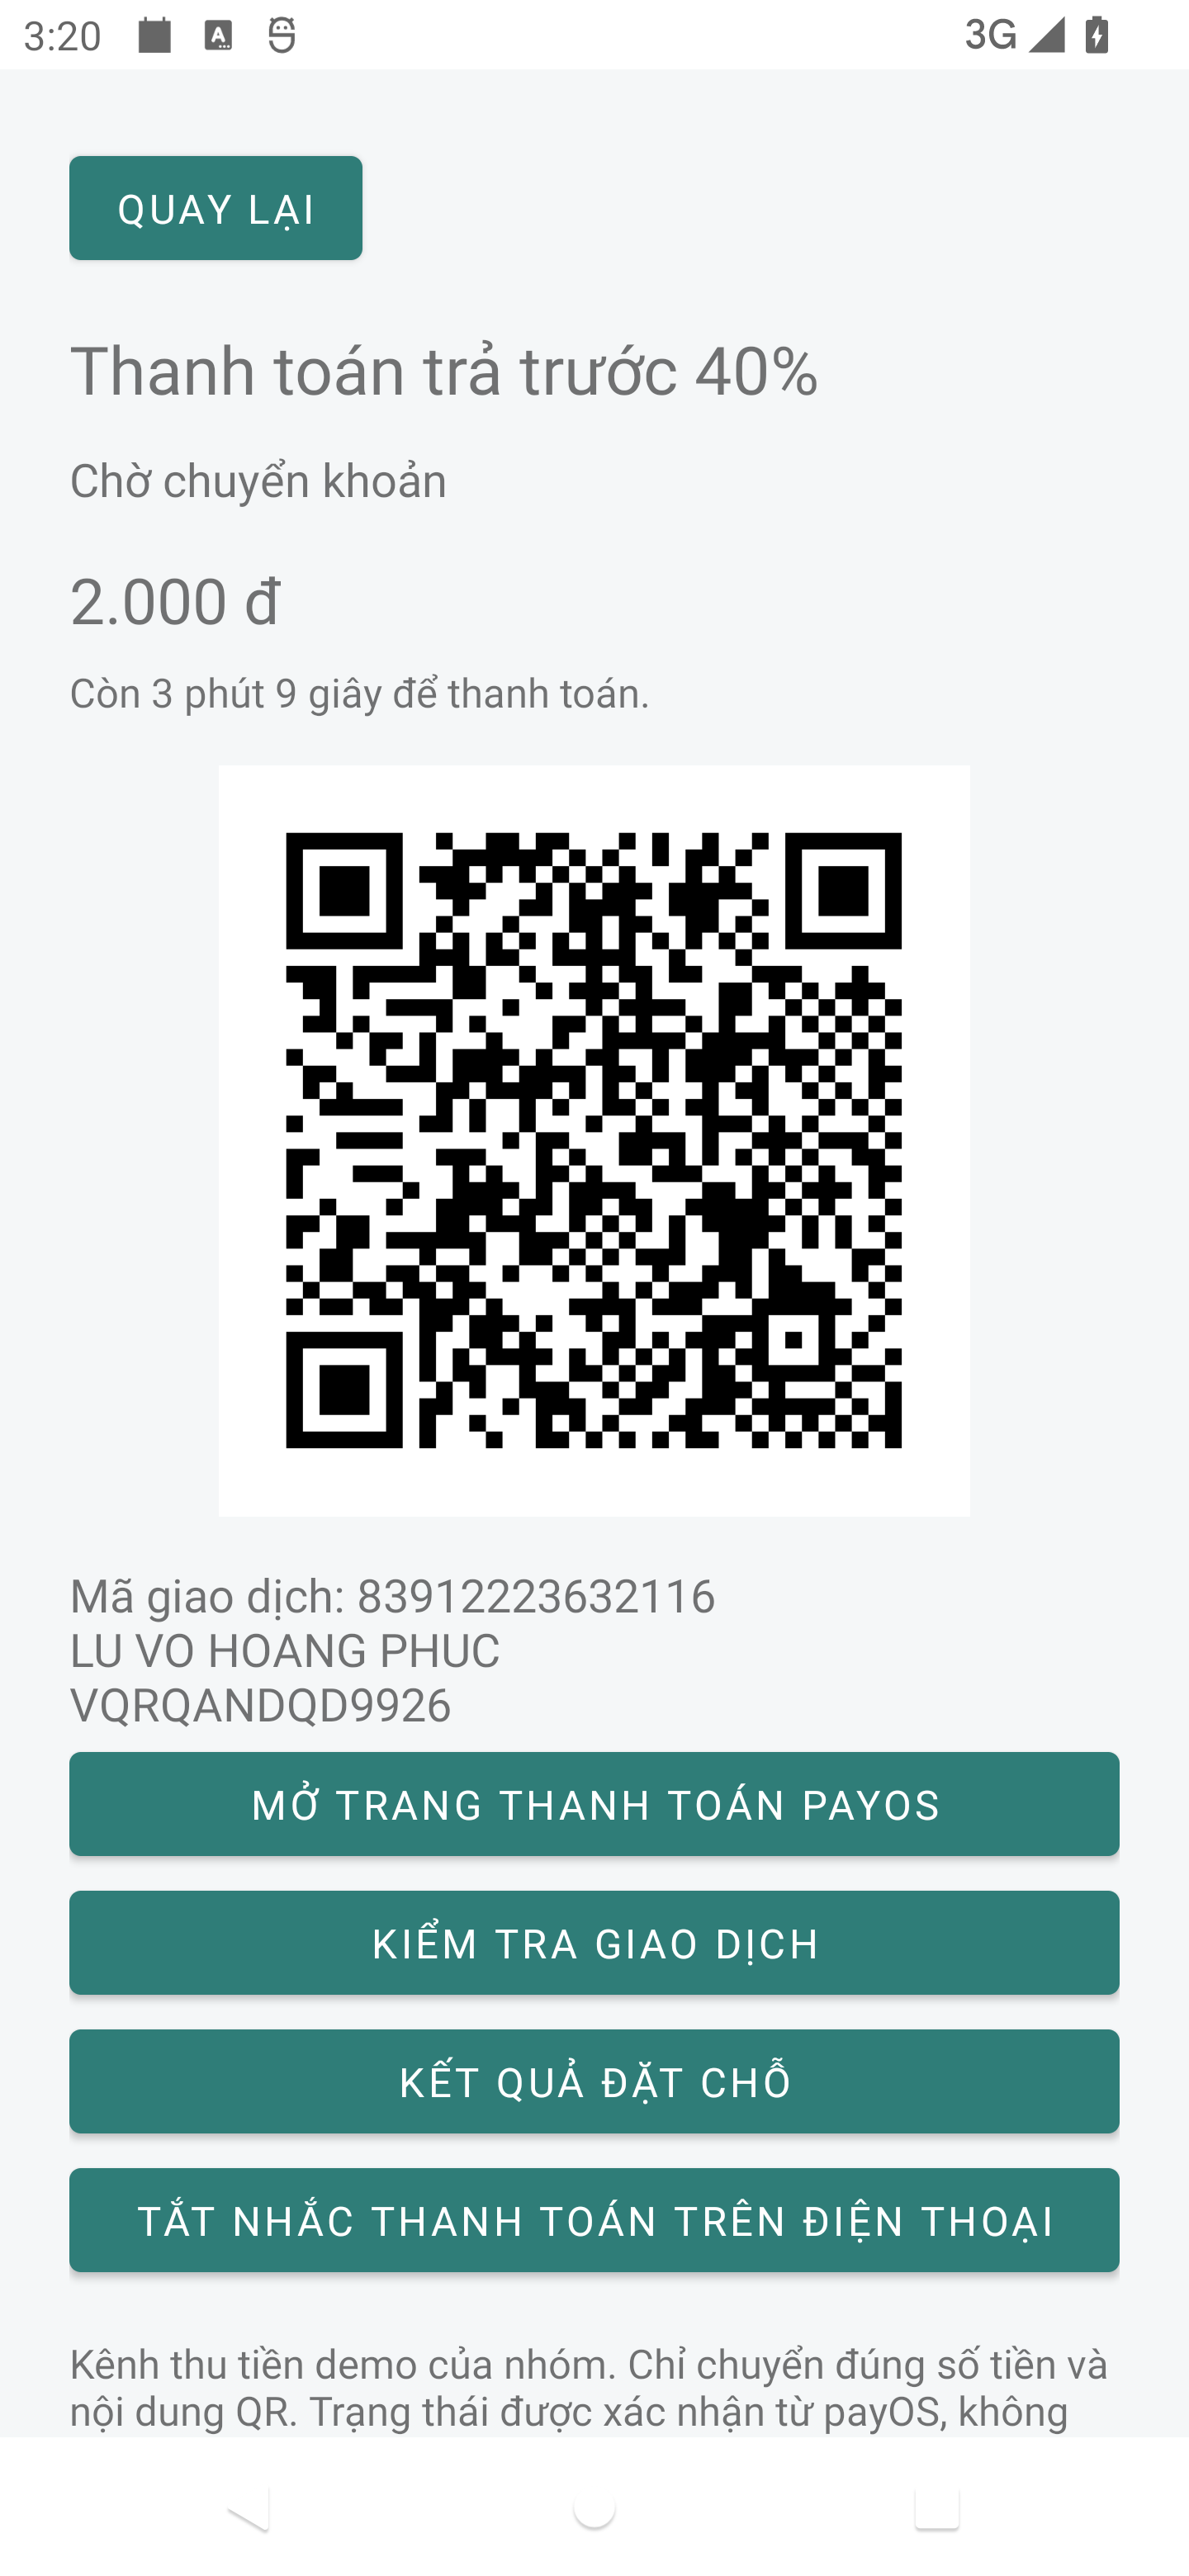
\includegraphics[width=\linewidth]{chapter6/booking-qr.png}\\[-1mm]
{\small (b) Phiên QR có thời hạn}
\end{minipage}
\caption{Từ kết quả kiểm tra lịch đến phiên thanh toán QR}
\label{fig:booking-quote-qr}
\end{minipage}
\end{figure}}{}

Khi payOS gửi dữ liệu thanh toán, webhook được chuyển tới backend BroomSharing để xác thực và đối soát. Backend kiểm tra giao dịch, số tiền và thời điểm thanh toán trước khi cập nhật trạng thái. Nhận đủ 40\% đúng hạn mới chuyển booking sang CONFIRMED và ghi nhận PAID; lịch đang giữ tiếp tục thuộc booking đó. Listener cập nhật kết quả trên Android, đồng thời thông báo thanh toán được đổi trạng thái. Booking không cần Host duyệt trước bước này.

\IfFileExists{Resources/chapter6/booking-paid.png}{%
\begin{figure}[H]
\begin{minipage}{\linewidth}
\setlength{\parindent}{1.27cm}
\setstretch{1.4}
Hình~\ref{fig:booking-payment-outcomes} ghi nhận hai kết quả ở hai giao dịch khác nhau. Ở Hình~\ref{fig:booking-payment-outcomes}(a), giao dịch đã nhận 2.000 đồng và booking được xác nhận. Ở Hình~\ref{fig:booking-payment-outcomes}(b), người thuê chưa trả tiền khi hết năm phút; backend khép booking EXPIRED, nhả lịch và ứng dụng hiển thị đặt chỗ không thành công. QR hết hạn được gỡ khỏi màn hình, thông báo điện thoại đổi sang kết quả thất bại. Nút xem kết quả đưa người thuê tới chi tiết booking để theo dõi trạng thái cuối.
\par\medskip
\centering
\begin{minipage}[t]{0.40\linewidth}\centering
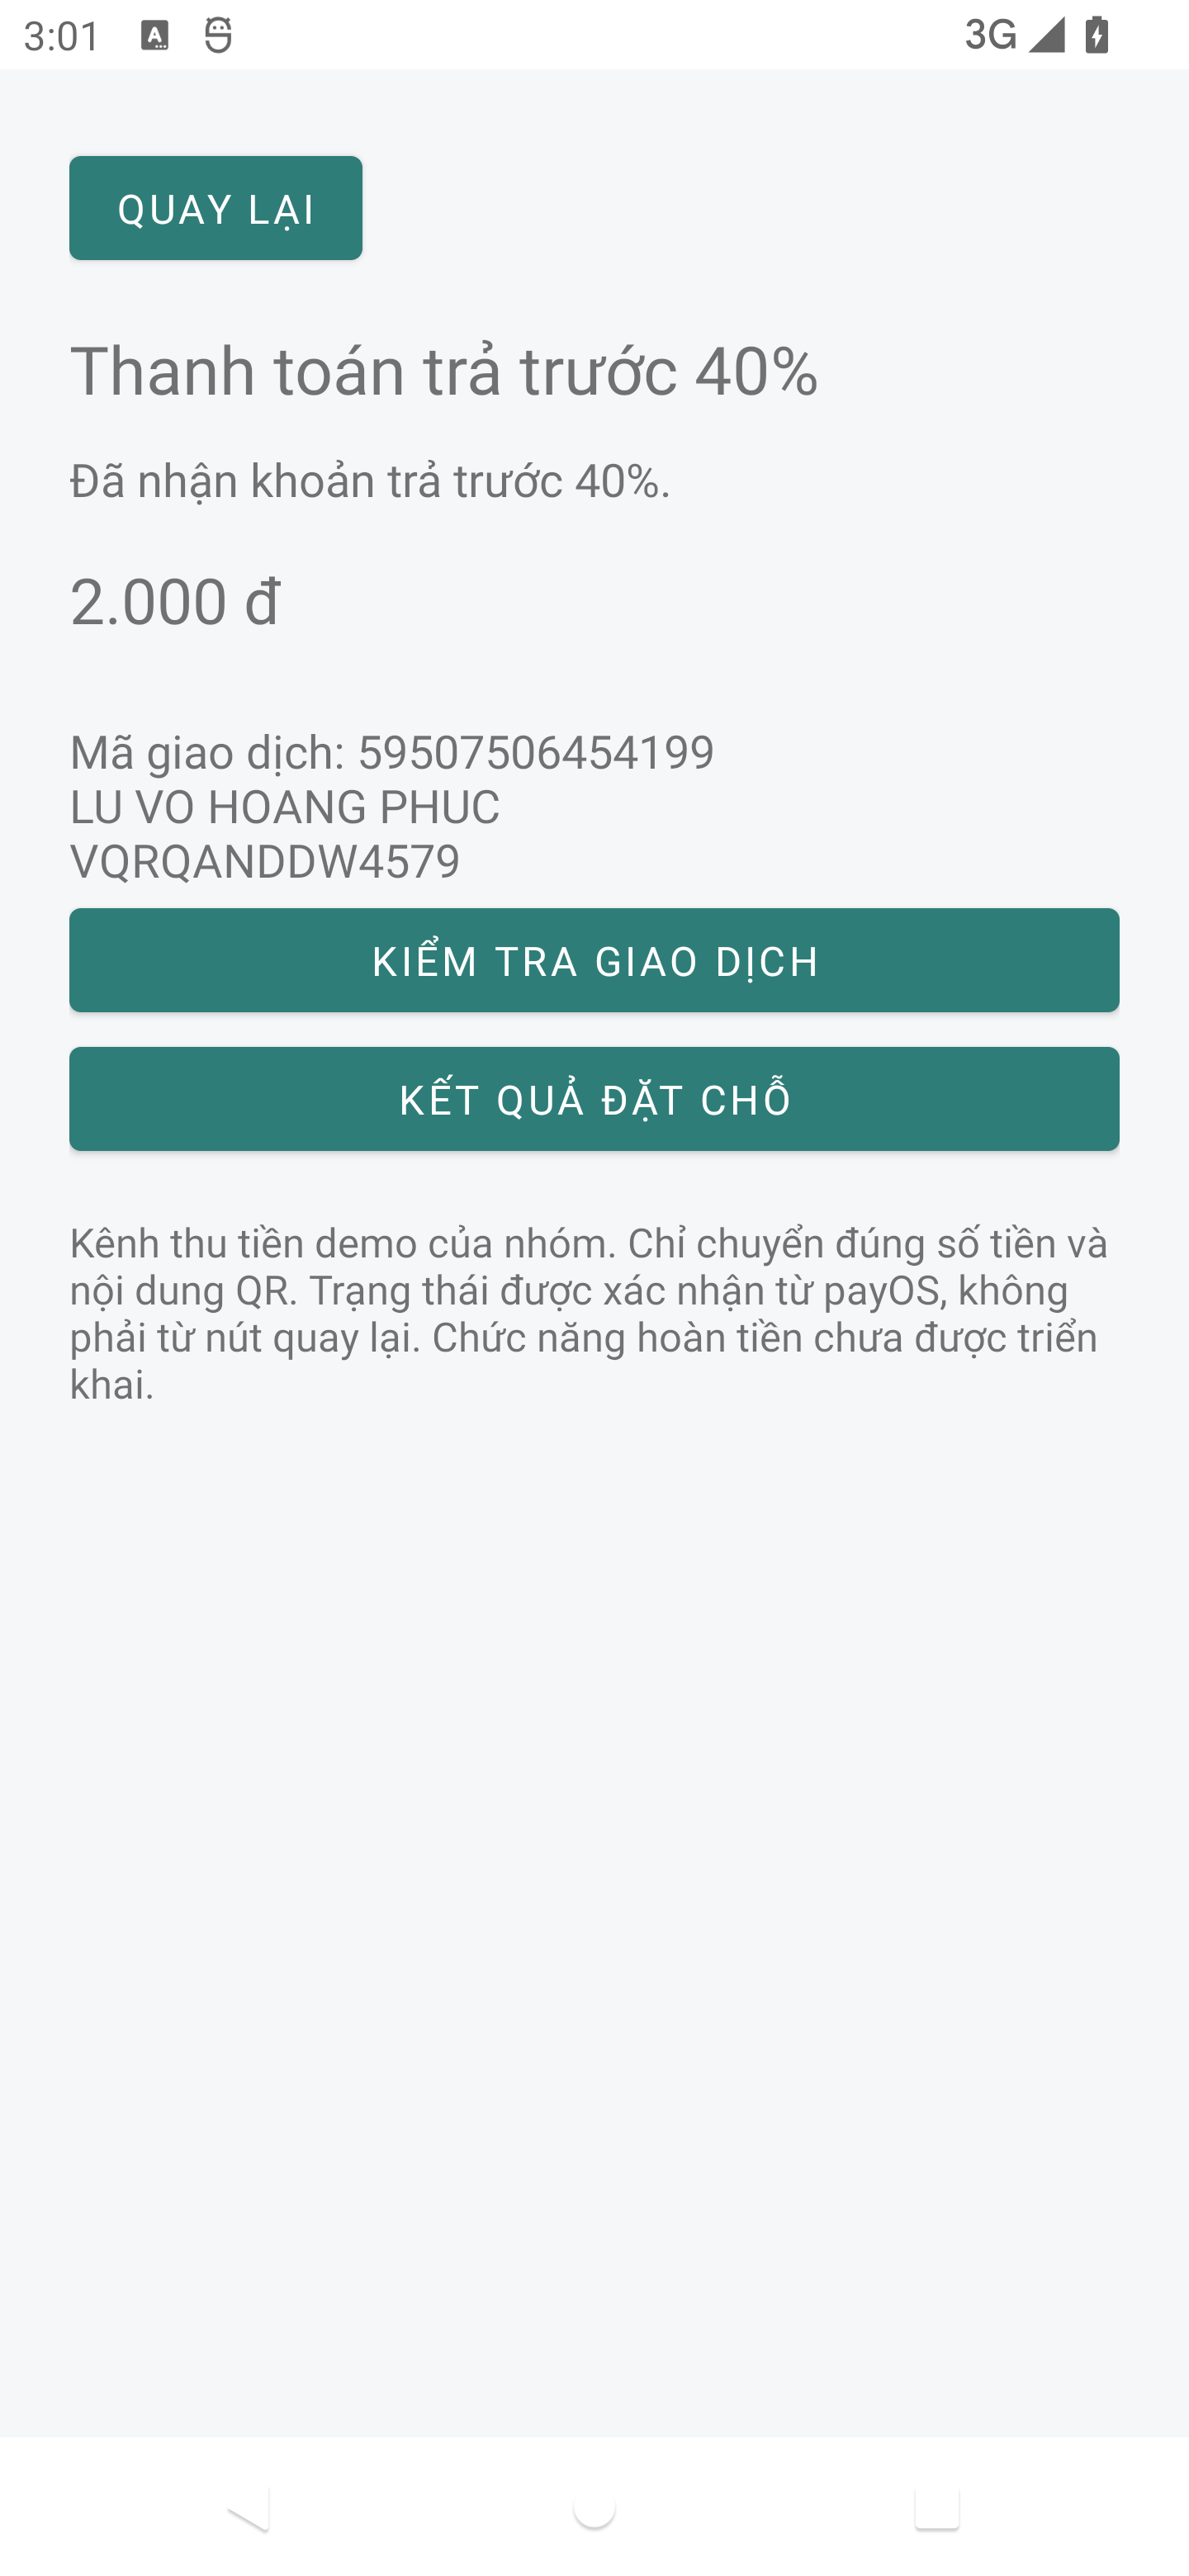
\includegraphics[width=\linewidth]{chapter6/booking-paid.png}\\[-1mm]
{\small (a) Đã ghi nhận thanh toán}
\end{minipage}\hspace{0.05\linewidth}%
\begin{minipage}[t]{0.40\linewidth}\centering
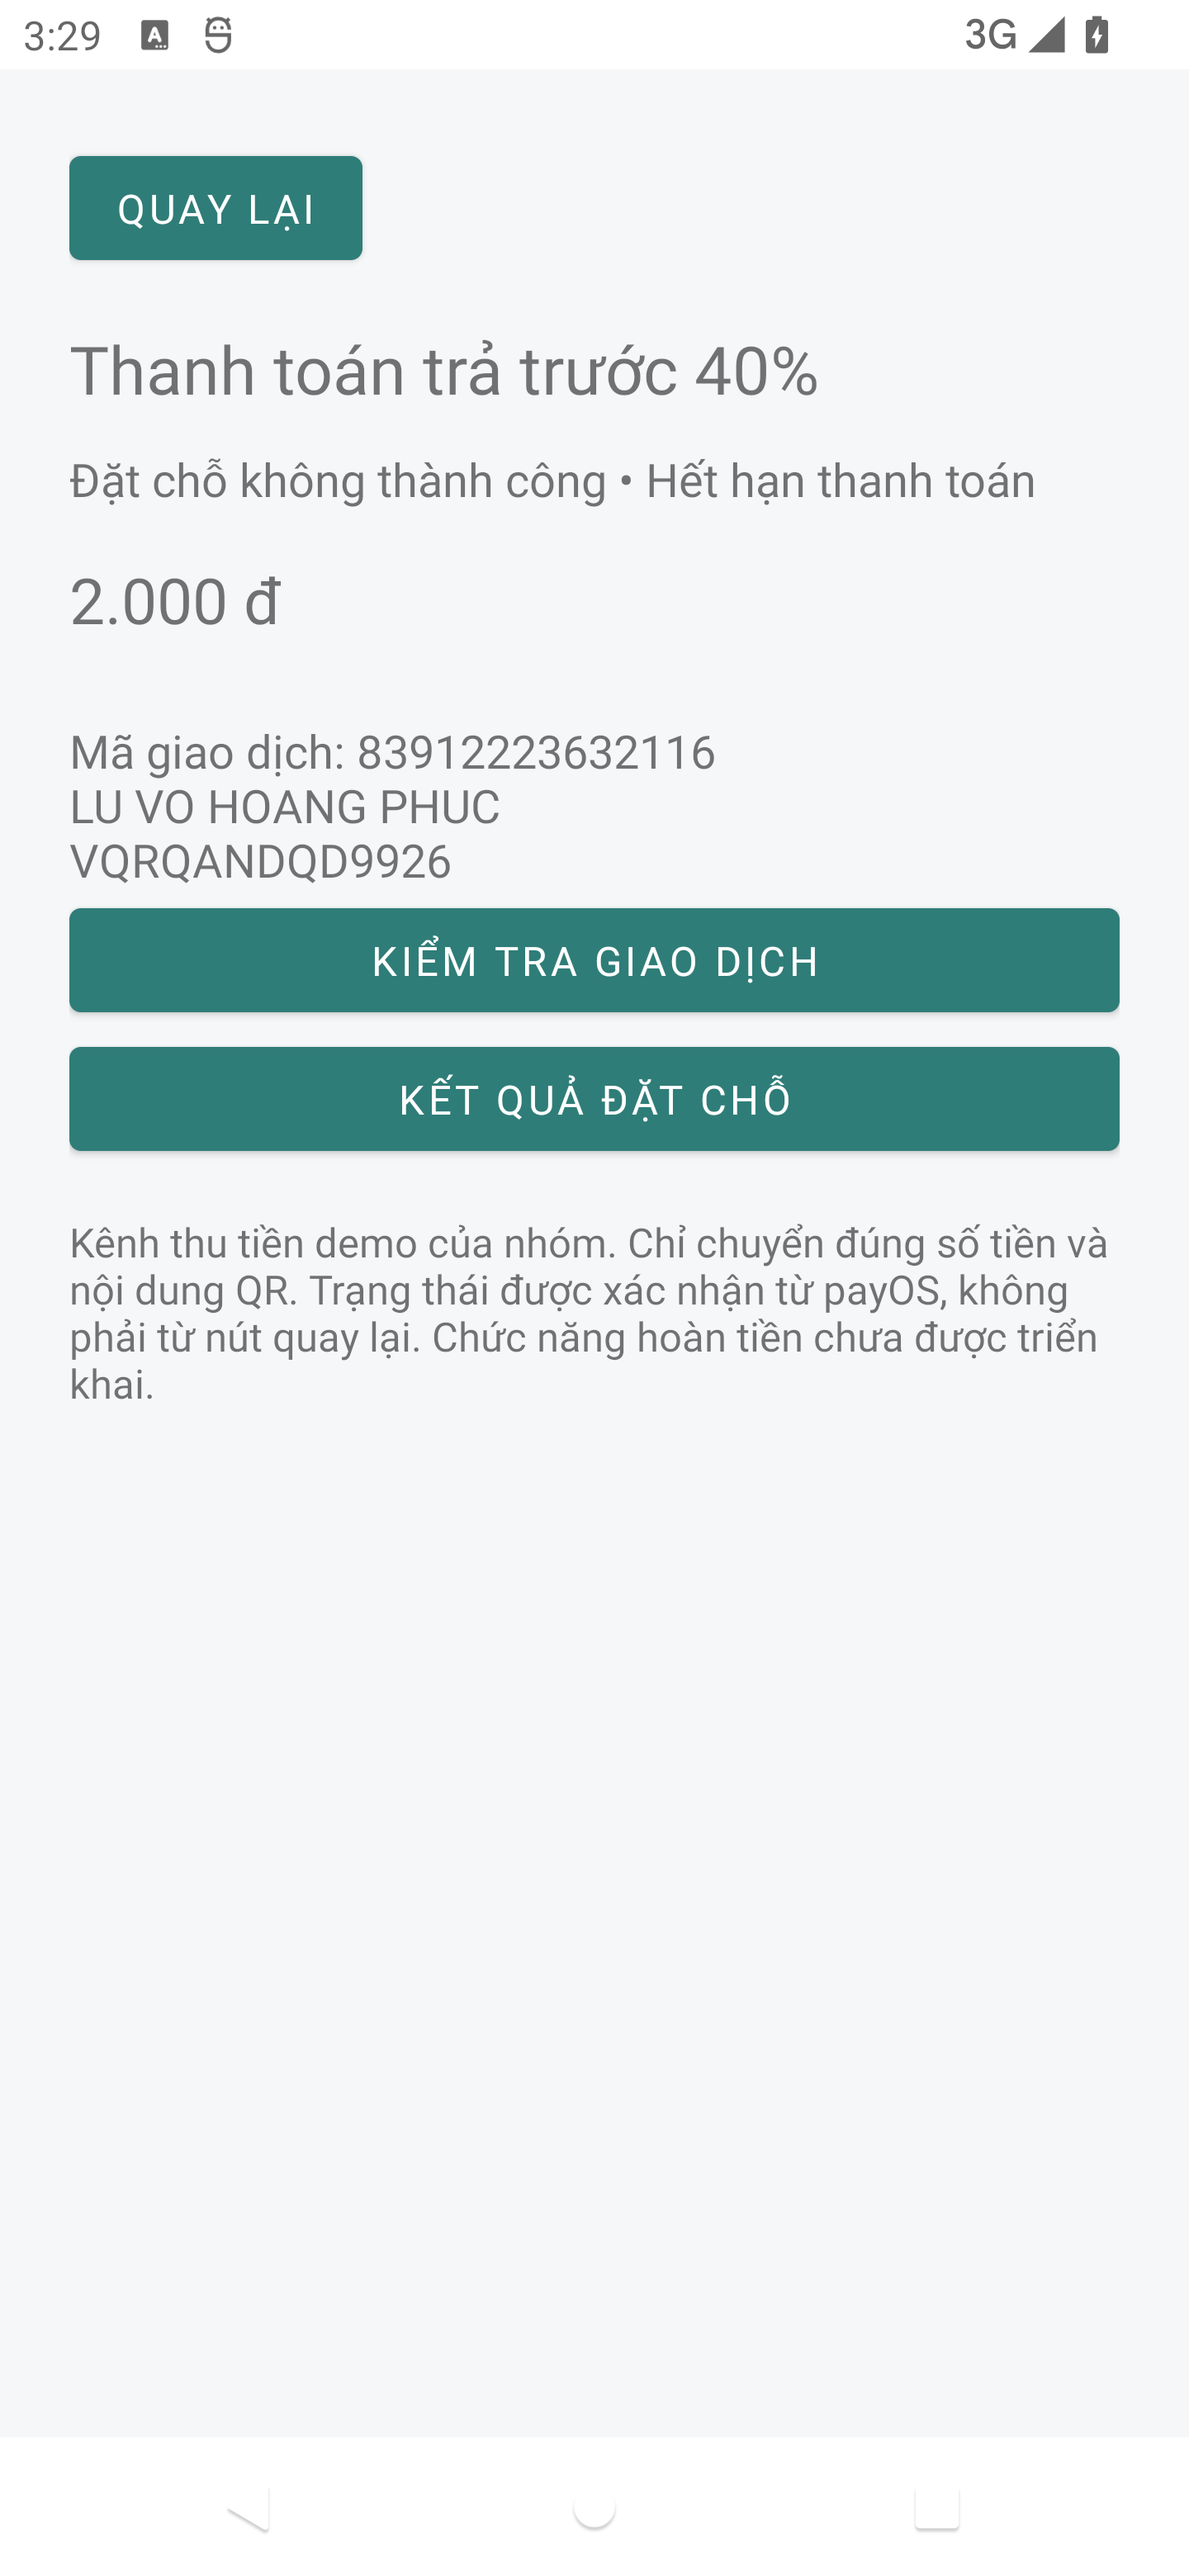
\includegraphics[width=\linewidth]{chapter6/booking-expired.png}\\[-1mm]
{\small (b) Hết hạn chưa thanh toán}
\end{minipage}
\caption{Kết quả xác nhận và hết hạn của các phiên đặt chỗ}
\label{fig:booking-payment-outcomes}
\end{minipage}
\end{figure}}{}

Người thuê theo dõi trạng thái cuối tại danh sách và chi tiết đặt chỗ. Trường hợp nhận tiền muộn hoặc dữ liệu tiền cần kiểm tra không được tự chuyển thành đã xác nhận; hệ thống giữ thông tin để đối soát thủ công. Phiên bản đồ án chưa thực hiện hoàn tiền qua API. Xác nhận thanh toán cũng không tự ghi khách đã đến hoặc đã sử dụng phòng; các mốc nhận phòng và hoàn tất thuộc quá trình thực hiện lượt thuê.

\clearpage
\noindent\begin{minipage}{\linewidth}
\captionsetup{hypcap=false}
\setstretch{1.4}
\noindent Hình~\ref{fig:booking-resume-notification}(a) cho thấy thẻ tiếp tục thanh toán khi một phiên còn hiệu lực. Người thuê chạm nút để mở lại đúng giao dịch với thời gian còn lại, thay vì chọn ngày và tạo booking mới. Thẻ chỉ xuất hiện khi có phiên đang chờ. Khi đã xác định hết hạn chưa trả tiền, thông báo điện thoại đổi sang đặt chỗ không thành công như Hình~\ref{fig:booking-resume-notification}(b); chạm thông báo mở kết quả liên quan. Bộ đếm tại thiết bị chỉ hỗ trợ hiển thị, còn kết quả tiền và việc nhả lịch do backend đối soát.
\par\medskip
\centering
\begin{minipage}[t]{0.40\linewidth}\centering
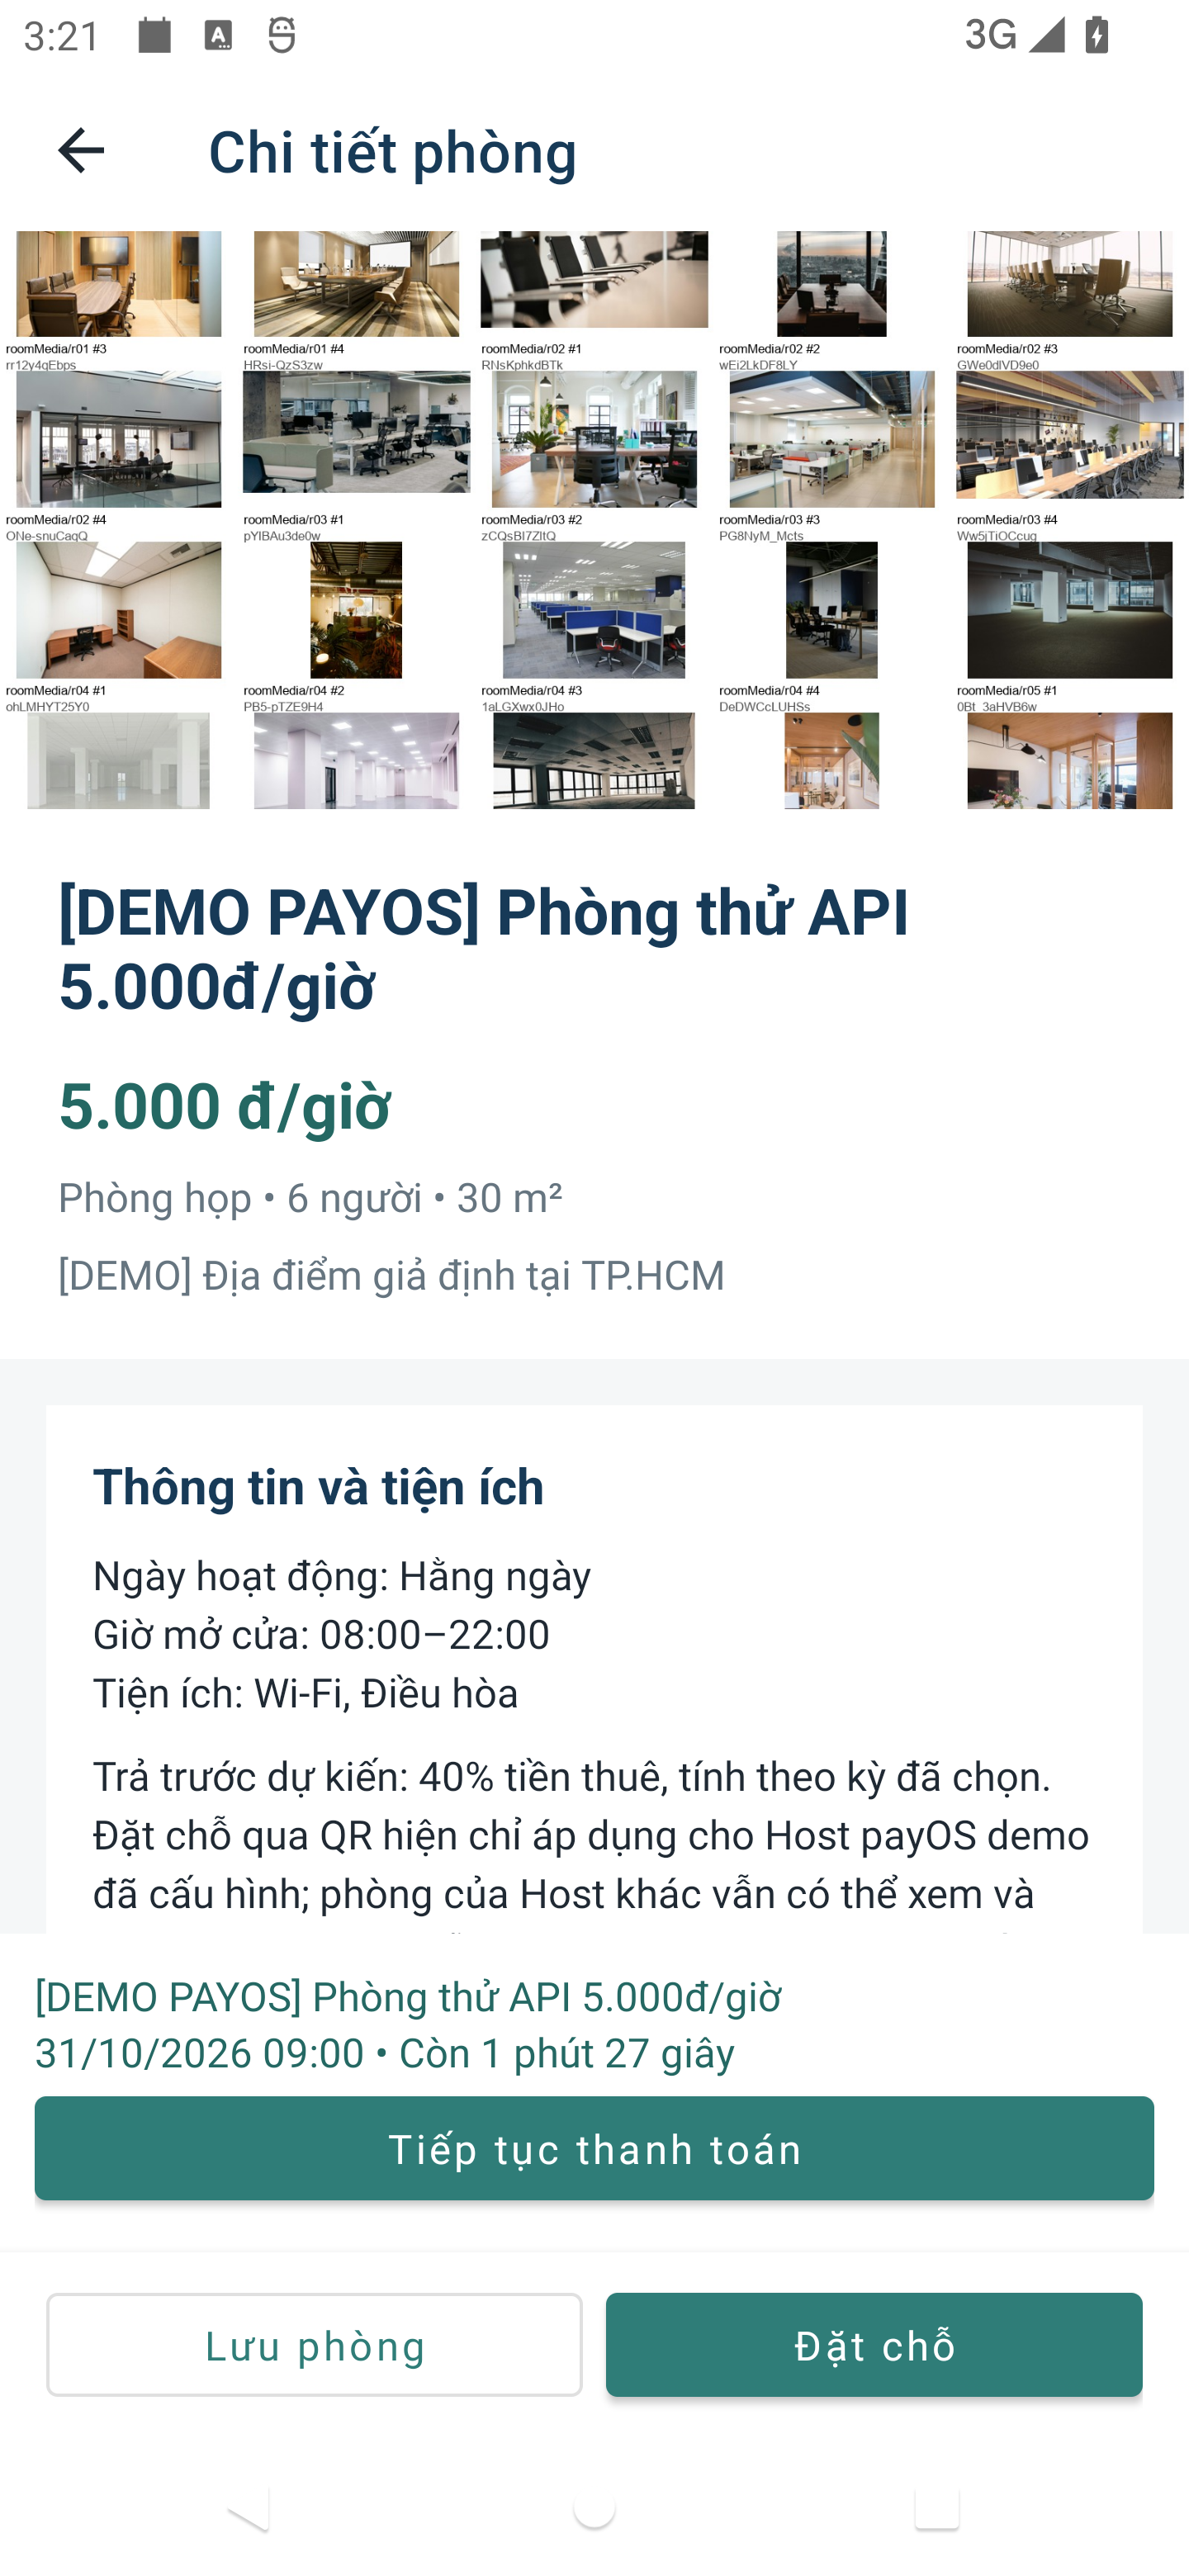
\includegraphics[width=\linewidth]{chapter6/booking-resume.png}\\[-1mm]
{\small (a) Tiếp tục phiên còn hạn}
\end{minipage}\hspace{0.05\linewidth}%
\begin{minipage}[t]{0.40\linewidth}\centering
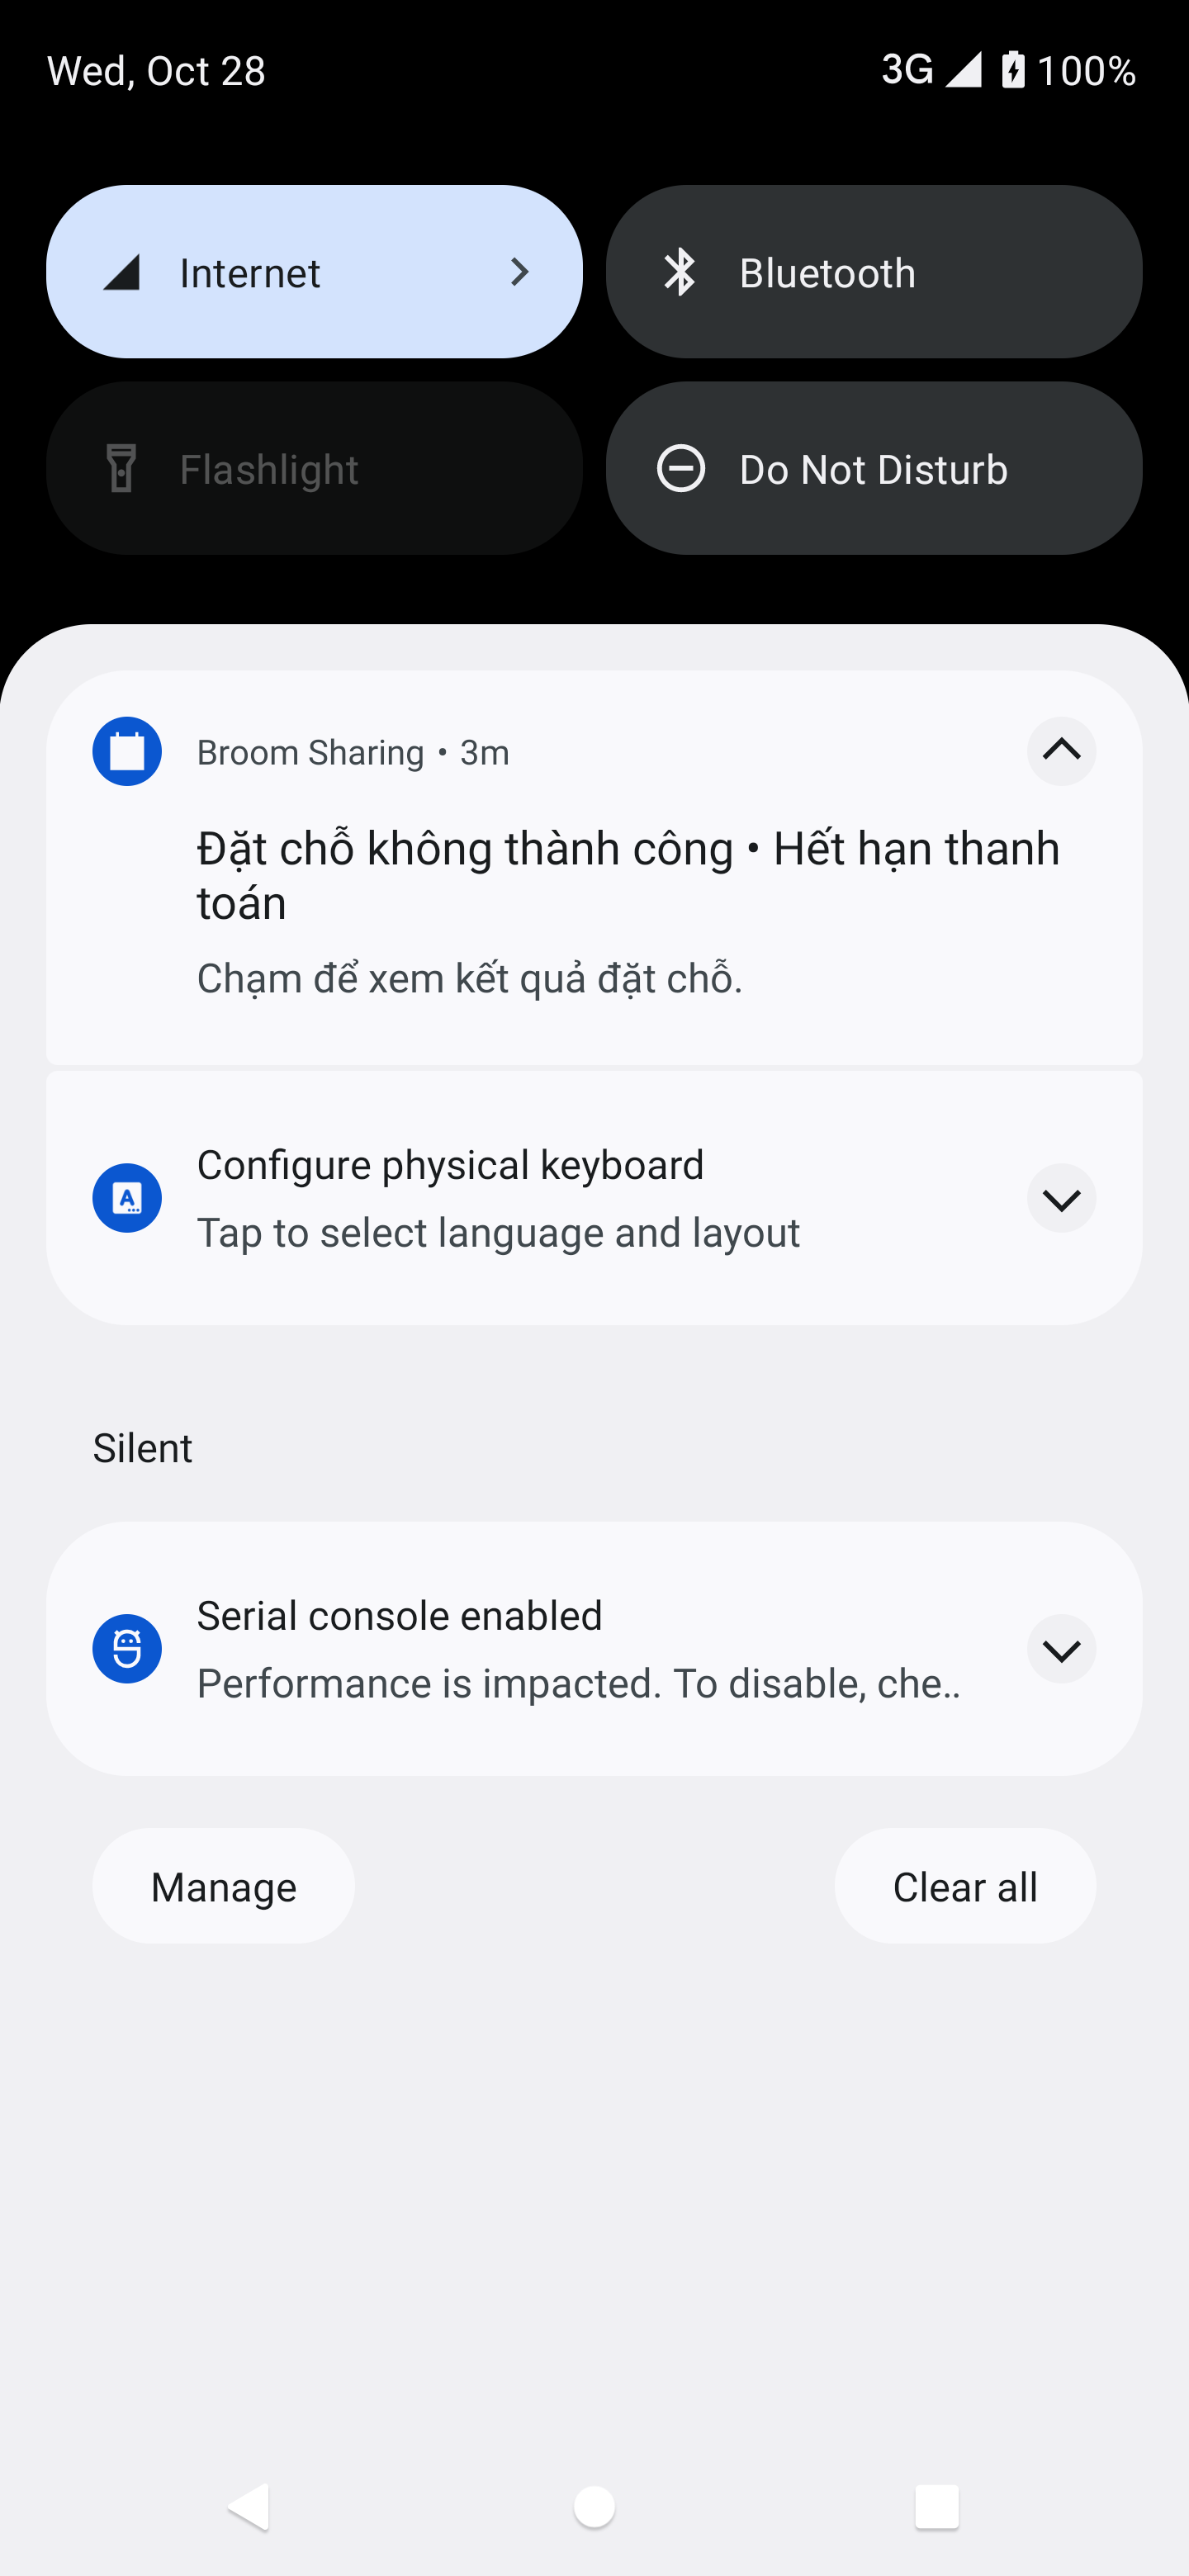
\includegraphics[width=\linewidth]{chapter6/booking-phone-notification.png}\\[-1mm]
{\small (b) Thông báo kết quả hết hạn}
\end{minipage}
\captionof{figure}{Tiếp tục giao dịch và nhận kết quả qua thông báo điện thoại}
\label{fig:booking-resume-notification}
\end{minipage}
\par

\Needspace{0.55\textheight}
\subsection{Quy trình thực hiện lượt thuê và đánh giá}
Điều kiện bắt đầu là booking đã xác nhận và còn thuộc các bên tham gia. Người thuê xem lại thời gian, địa chỉ, liên hệ trong chi tiết; Host theo dõi lịch phòng và danh sách lượt thuê. Trình tự sử dụng thông thường gồm:
\begin{enumerate}
\item Khi khách đến trong kỳ thuê, Host ghi nhận nhận phòng. Booking chuyển từ CONFIRMED sang CHECKED\_IN và lưu căn cứ sử dụng; thao tác này độc lập với QR thanh toán.
\item Sau giờ kết thúc, Host hoàn tất lượt đã sử dụng. Booking chuyển COMPLETED, giải phóng khóa lịch tương ứng, cập nhật dữ liệu phòng và lưu audit, đồng thời giữ lịch sử.
\item Người thuê mở đánh giá từ lượt đủ điều kiện, chọn điểm 1 đến 5 và nhập nhận xét. Hệ thống kiểm tra lại Guest, trạng thái khép và xác nhận sử dụng trước khi lưu một đánh giá cho booking đó.
\end{enumerate}

Lịch tháng tại Hình~\ref{fig:actual-host-calendar} giúp Host chọn ngày và kiểm tra khoảng đã giữ. Nếu khách không đến, sau giờ kết thúc Host ghi NO\_SHOW kèm lý do; lượt này không tự có quyền đánh giá. Với lượt đã dùng nhưng thiếu thao tác nhận phòng, cần xác minh sử dụng trước khi hoàn tất, không suy ra việc sử dụng chỉ vì thời gian đã qua.

Khi phát sinh vấn đề, người thuê gửi báo cáo và theo dõi kết quả; Host phản hồi hồ sơ còn mở, Admin kết luận theo phạm vi quản trị. Nếu Host bị khóa, Admin xem xét từng booking: có thể hủy lượt chưa nhận phòng hoặc kết thúc lượt đang sử dụng do sự cố ở trạng thái TERMINATED, kèm lý do và audit. Việc xác minh lại lượt đã khép không nhả lịch lần thứ hai. Các quyết định này không đồng nghĩa đã hoàn tiền; giao dịch liên quan phải được đối soát riêng.

Khi mất kết nối, người thuê vẫn mở được lịch sử và chi tiết booking đã tải từ SQLite, như Hình~\ref{fig:sqlite-offline-screens}(b). Màn hình ghi thời điểm bản lưu và chỉ cho xem thông tin. Khi kết nối trở lại, ứng dụng kiểm tra phiên rồi cập nhật dữ liệu từ Firestore trước khi cho phép thực hiện các thao tác trực tuyến.

\endgroup

\chapstart
\section{KẾT LUẬN VÀ HƯỚNG MỞ RỘNG}
\subsection{Kết quả đạt được}
BroomSharing được xây dựng bằng Java và XML theo MVVM + Repository + Model, kết nối người thuê, Host và Admin trong các luồng tìm không gian, quản lý tài sản, đặt chỗ và kiểm duyệt. Cloud Firestore lưu dữ liệu theo collection, document và subcollection, liên kết tài khoản, phòng và lịch bằng ID. Giao diện quan sát trạng thái, còn Repository tập trung thao tác dữ liệu.

Luồng đặt chỗ kết nối backend Java với payOS, tạm giữ lịch tối đa năm phút và xác nhận sau khi đối soát đủ khoản trả trước 40\%. Transaction kiểm soát booking và lịch; giao diện phân biệt thanh toán, hết hạn và khép lượt. Bản đồ, ảnh trực tuyến, chat và đánh giá hỗ trợ quá trình thuê; kênh Admin lưu quyết định cùng nhật ký để đối chiếu. SQLite cho phép xem lại thông tin phòng và đặt chỗ đã tải khi thiết bị mất mạng.

\subsection{Những hạn chế hiện tại}
Thanh toán giới hạn ở một kênh Host demo, với backend Java chạy trên máy của nhóm qua đường hầm kết nối. Đối soát ngoại lệ và hoàn tiền được xử lý thủ công ngoài ứng dụng. Hồ sơ Host dùng giấy tờ DEMO và được Admin xét duyệt bằng người; phạm vi này không bao gồm định danh pháp lý hoặc lưu trữ giấy tờ cá nhân thật.

Dữ liệu ngoại tuyến phản ánh lần tải gần nhất. Kiểm tra lịch trống, đặt chỗ và thanh toán sử dụng dữ liệu trực tuyến; bản đồ và tính tuyến đường phụ thuộc dịch vụ bên ngoài.

Sự kiện trên lịch điện thoại được lưu qua biểu mẫu xác nhận của người dùng và quản lý độc lập với các thay đổi của booking.

\subsection{Hướng phát triển}
Ưu tiên là triển khai backend tại địa chỉ ổn định, lưu tệp định danh riêng tư và hoàn thiện đối soát, hoàn tiền theo khả năng nhà cung cấp. Thanh toán nhiều Host cần có quy trình đăng ký và kiểm tra bên nhận tiền.

Ở phía ứng dụng, có thể mở rộng dữ liệu được lưu ngoại tuyến và cập nhật lịch điện thoại theo thay đổi của booking. Khi quy mô tăng, cần tiếp tục tối ưu lượt đọc, phạm vi listener và tìm kiếm theo vị trí, đồng thời bảo đảm tính nhất quán của lịch và quyền truy cập.

\clearpage
\phantomsection
\printbibliography[heading=bibintoc,title={TÀI LIỆU THAM KHẢO}]
\clearpage
\pagestyle{plain}
\section*{PHỤ LỤC A. DANH MỤC HÌNH VÀ BẢNG}
\phantomsection\addcontentsline{toc}{section}{PHỤ LỤC A. DANH MỤC HÌNH VÀ BẢNG}
\printappendixfigures
\medskip
\printappendixtables

\clearpage
\section*{PHỤ LỤC B. PROTOTYPE QUẢN TRỊ}
\phantomsection\addcontentsline{toc}{section}{PHỤ LỤC B. PROTOTYPE QUẢN TRỊ}
\setcounter{figure}{0}\renewcommand{\thefigure}{B.\arabic{figure}}
Hình~\ref{fig:app-admin-design} minh họa hai nhóm nội dung kiểm duyệt phòng và quản lý tài khoản. Thẻ thông tin đặt thao tác chấp thuận, từ chối hoặc quản lý trạng thái cạnh đối tượng cần xử lý. Phần tổng quan và bộ lọc hỗ trợ xác định nhóm hồ sơ trước khi mở chi tiết; số liệu trong hình là dữ liệu minh họa thiết kế.
\begin{figure}[H]\centering
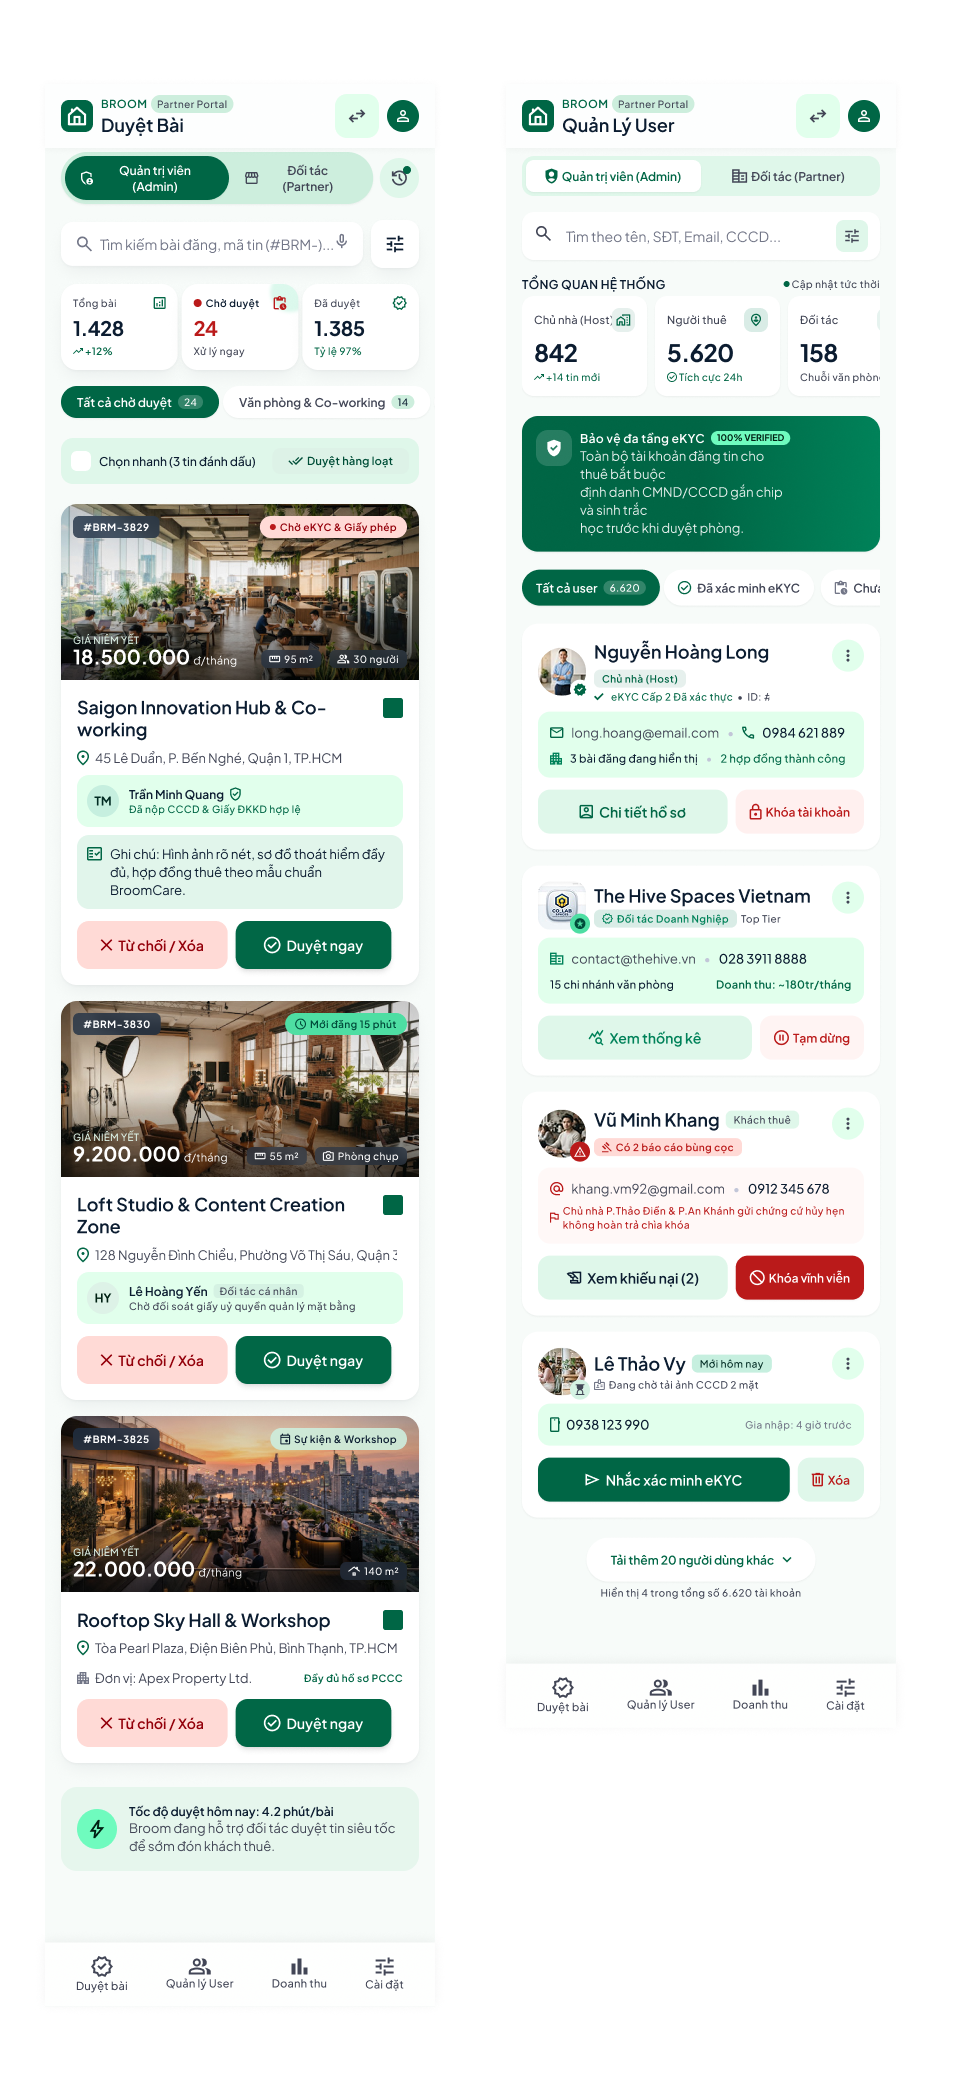
\includegraphics[width=\textwidth,height=0.63\textheight,keepaspectratio]{chapter3/admin-design.png}
\caption{Phương án thiết kế kiểm duyệt và quản lý trong phân hệ Admin.}\label{fig:app-admin-design}
\end{figure}

\clearpage


\clearpage
\section*{PHỤ LỤC C. LIÊN KẾT VÀ PHÂN CÔNG BÁO CÁO}
\phantomsection\addcontentsline{toc}{section}{PHỤ LỤC C. LIÊN KẾT VÀ PHÂN CÔNG BÁO CÁO}
\label{app:project-resources}
\setcounter{table}{0}\renewcommand{\thetable}{C.\arabic{table}}
\subsection*{Đường dẫn GitHub}
\begin{center}
\href{https://github.com/phuclu3123/GROUP_MOBILE_BROOMSHARING.git}{\textcolor{uehblue}{\faGithub\hspace{0.25cm}Nhấn vào đây để mở GITHUB}}
\end{center}

\subsection*{Excel phân công công việc}
\begin{center}
\href{https://drive.google.com/file/d/1QgZXFG2qhMrYj7dkOfLZZZsQbiwZeeLu/view?usp=drive_link}{\textcolor{uehblue}{\faFileExcel\hspace{0.25cm}Nhấn vào đây để mở EXCEL phân chia công việc}}
\end{center}

\subsection*{Asset hình ảnh ứng dụng và sơ đồ}
\begin{center}
\href{https://drive.google.com/drive/folders/17oHiO-325_xpyVXmavMDbLrI7sBT2iks?usp=drive_link}{\textcolor{uehblue}{\faImages\hspace{0.25cm}Nhấn vào đây để mở ASSET hình ảnh ứng dụng và sơ đồ}}
\end{center}

\subsection*{Thiết kế giao diện Figma}
\begin{center}
\href{https://www.figma.com/design/OAJ9pPqR3CWAcIfSuo5s3r/Untitled?node-id=0-1\&t=u8GIv9DUp24mnwg1-1}{\textcolor{uehblue}{\faFigma\hspace{0.25cm}Nhấn vào đây để mở FIGMA}}
\end{center}

\subsection*{Video demo sản phẩm}
\begin{center}
\href{https://youtube.com/playlist?list=PLa4LDgd4xXAo\&si=vXRBWmxMzxkjoVV5}{\textcolor{uehblue}{\faYoutube\hspace{0.25cm}Video demo sản phẩm}}
\end{center}

\noindent Bảng~\ref{tab:team-responsibilities} tóm tắt phân công viết các chương và mục trong báo cáo.

\begin{table}[H]\centering\small
\caption{Phân công viết báo cáo}\label{tab:team-responsibilities}
\begin{tabularx}{\linewidth}{@{}p{4.5cm}X@{}}\toprule
Thành viên & Phần báo cáo phụ trách\\\midrule
Lữ Võ Hoàng Phúc & Chương 4 và 7; các mục 5.1, 5.2, 5.3.8 và 6.4; phần Admin trong mục 5.4.\\
Lâm Hoàng & Chương 2; các mục 5.3.7, 6.1, 6.3 và 6.5; phần Host trong mục 5.4.\\
Từ Trương Thanh Trúc & Chương 1 và 3; các mục 5.3.1 đến 5.3.6 và 6.2; phần người thuê trong mục 5.4.\\
\bottomrule\end{tabularx}
\end{table}

\end{document}
